\documentclass{article}

% TODO : CLEAN UP THIS MESS
% (AND MAKE SURE ALL TEXTS STILL COMPILE)
\usepackage[leqno]{amsmath}
\usepackage{amssymb}
\usepackage{graphicx}

\usepackage{diagbox} % table heads with diagonal lines
\usepackage{relsize}

\usepackage{wasysym}
\usepackage{scrextend}
\usepackage{epigraph}
\setlength\epigraphwidth{.6\textwidth}

\usepackage[utf8]{inputenc}

\usepackage{titlesec}
\titleformat{\chapter}[display]
  {\normalfont\sffamily\huge\bfseries}
  {\chaptertitlename\ \thechapter}{5pt}{\Huge}
\titleformat{\section}
  {\normalfont\sffamily\Large\bfseries}
  {\thesection}{1em}{}
\titleformat{\subsection}
  {\normalfont\sffamily\large\bfseries}
  {\thesubsection}{1em}{}
\titleformat{\part}[display]
  {\normalfont\sffamily\huge\bfseries}
  {\partname\ \thepart}{0pt}{\Huge}

\usepackage[T1]{fontenc}
\usepackage{fourier}
\usepackage{paratype}

\usepackage[symbol,perpage]{footmisc}

\usepackage{perpage}
\MakePerPage{footnote}

\usepackage{array}
\newcolumntype{x}[1]{>{\centering\hspace{0pt}}p{#1}}

% TODO: the following line causes conflict with new texlive (!)
% \usepackage[english,russian,polutonikogreek,spanish]{babel}
% \newcommand{\russian}[1]{{\selectlanguage{russian}#1}}

% Remove conflicting options for the moment:
\usepackage[english,polutonikogreek,spanish]{babel}

\AtBeginDocument{\shorthandoff{"}}
\newcommand{\greek}[1]{{\selectlanguage{polutonikogreek}#1}}

% % % % % % % % % % % % % % % % % % % % % % % % % % % % % %
% Limit/colimit symbols (with accented i: lím / colím)

\usepackage{etoolbox} % \patchcmd

\makeatletter
\patchcmd{\varlim@}{lim}{\lim}{}{}
\makeatother
\DeclareMathOperator*{\colim}{co{\lim}}
\newcommand{\dirlim}{\varinjlim}
\newcommand{\invlim}{\varprojlim}

% % % % % % % % % % % % % % % % % % % % % % % % % % % % % %

\usepackage[all,color]{xy}

\usepackage{pigpen}
\newcommand{\po}{\ar@{}[dr]|(.4){\text{\pigpenfont I}}}
\newcommand{\pb}{\ar@{}[dr]|(.3){\text{\pigpenfont A}}}
\newcommand{\polr}{\ar@{}[dr]|(.65){\text{\pigpenfont A}}}
\newcommand{\pour}{\ar@{}[ur]|(.65){\text{\pigpenfont G}}}
\newcommand{\hstar}{\mathop{\bigstar}}

\newcommand{\bigast}{\mathop{\Huge \mathlarger{\mathlarger{\ast}}}}

\newcommand{\term}{\textbf}

\usepackage{stmaryrd}

\usepackage{cancel}

\usepackage{tikzsymbols}

\newcommand{\open}{\underset{\mathrm{open}}{\hookrightarrow}}
\newcommand{\closed}{\underset{\mathrm{closed}}{\hookrightarrow}}

\newcommand{\tcol}[2]{{#1 \choose #2}}

\newcommand{\homot}{\simeq}
\newcommand{\isom}{\cong}
\newcommand{\cH}{\mathcal{H}}
\renewcommand{\hom}{\mathrm{hom}}
\renewcommand{\div}{\mathop{\mathrm{div}}}
\renewcommand{\Im}{\mathop{\mathrm{Im}}}
\renewcommand{\Re}{\mathop{\mathrm{Re}}}
\newcommand{\id}[1]{\mathrm{id}_{#1}}
\newcommand{\idid}{\mathrm{id}}

\newcommand{\ZG}{{\ZZ G}}
\newcommand{\ZH}{{\ZZ H}}

\newcommand{\quiso}{\simeq}

\newcommand{\personality}[1]{{\sc #1}}

\newcommand{\mono}{\rightarrowtail}
\newcommand{\epi}{\twoheadrightarrow}
\newcommand{\xepi}[1]{\xrightarrow{#1}\mathrel{\mkern-14mu}\rightarrow}

% % % % % % % % % % % % % % % % % % % % % % % % % % % % % %

\DeclareMathOperator{\Ad}{Ad}
\DeclareMathOperator{\Aff}{Aff}
\DeclareMathOperator{\Ann}{Ann}
\DeclareMathOperator{\Aut}{Aut}
\DeclareMathOperator{\Br}{Br}
\DeclareMathOperator{\CH}{CH}
\DeclareMathOperator{\Cl}{Cl}
\DeclareMathOperator{\Coeq}{Coeq}
\DeclareMathOperator{\Coind}{Coind}
\DeclareMathOperator{\Cop}{Cop}
\DeclareMathOperator{\Corr}{Corr}
\DeclareMathOperator{\Cor}{Cor}
\DeclareMathOperator{\Cov}{Cov}
\DeclareMathOperator{\Der}{Der}
\DeclareMathOperator{\Div}{Div}
\DeclareMathOperator{\D}{D}
\DeclareMathOperator{\Ehr}{Ehr}
\DeclareMathOperator{\End}{End}
\DeclareMathOperator{\Eq}{Eq}
\DeclareMathOperator{\Ext}{Ext}
\DeclareMathOperator{\Frac}{Frac}
\DeclareMathOperator{\Frob}{Frob}
\DeclareMathOperator{\Funct}{Funct}
\DeclareMathOperator{\Fun}{Fun}
\DeclareMathOperator{\GL}{GL}
\DeclareMathOperator{\Gal}{Gal}
\DeclareMathOperator{\Gr}{Gr}
\DeclareMathOperator{\Hol}{Hol}
\DeclareMathOperator{\Hom}{Hom}
\DeclareMathOperator{\Ho}{Ho}
\DeclareMathOperator{\Id}{Id}
\DeclareMathOperator{\Ind}{Ind}
\DeclareMathOperator{\Inn}{Inn}
\DeclareMathOperator{\Isom}{Isom}
\DeclareMathOperator{\Ker}{Ker}
\DeclareMathOperator{\Lan}{Lan}
\DeclareMathOperator{\Lie}{Lie}
\DeclareMathOperator{\Map}{Map}
\DeclareMathOperator{\Mat}{Mat}
\DeclareMathOperator{\Max}{Max}
\DeclareMathOperator{\Mor}{Mor}
\DeclareMathOperator{\Nat}{Nat}
\DeclareMathOperator{\Nrd}{Nrd}
\DeclareMathOperator{\Ob}{Ob}
\DeclareMathOperator{\Out}{Out}
\DeclareMathOperator{\PGL}{PGL}
\DeclareMathOperator{\PSL}{PSL}
\DeclareMathOperator{\PSU}{PSU}
\DeclareMathOperator{\Pic}{Pic}
\DeclareMathOperator{\RHom}{RHom}
\DeclareMathOperator{\Rad}{Rad}
\DeclareMathOperator{\Ran}{Ran}
\DeclareMathOperator{\Rep}{Rep}
\DeclareMathOperator{\Res}{Res}
\DeclareMathOperator{\SL}{SL}
\DeclareMathOperator{\SO}{SO}
\DeclareMathOperator{\SU}{SU}
\DeclareMathOperator{\Sh}{Sh}
\DeclareMathOperator{\Sing}{Sing}
\DeclareMathOperator{\Specm}{Specm}
\DeclareMathOperator{\Spec}{Spec}
\DeclareMathOperator{\Sp}{Sp}
\DeclareMathOperator{\Stab}{Stab}
\DeclareMathOperator{\Sym}{Sym}
\DeclareMathOperator{\Tors}{Tors}
\DeclareMathOperator{\Tor}{Tor}
\DeclareMathOperator{\Tot}{Tot}
\DeclareMathOperator{\UUU}{U}

\DeclareMathOperator{\adj}{adj}
\DeclareMathOperator{\ad}{ad}
\DeclareMathOperator{\af}{af}
\DeclareMathOperator{\card}{card}
\DeclareMathOperator{\cm}{cm}
\DeclareMathOperator{\codim}{codim}
\DeclareMathOperator{\cod}{cod}
\DeclareMathOperator{\coeq}{coeq}
\DeclareMathOperator{\coim}{coim}
\DeclareMathOperator{\coker}{coker}
\DeclareMathOperator{\cont}{cont}
\DeclareMathOperator{\conv}{conv}
\DeclareMathOperator{\cor}{cor}
\DeclareMathOperator{\depth}{depth}
\DeclareMathOperator{\diag}{diag}
\DeclareMathOperator{\diam}{diam}
\DeclareMathOperator{\dist}{dist}
\DeclareMathOperator{\dom}{dom}
\DeclareMathOperator{\eq}{eq}
\DeclareMathOperator{\ev}{ev}
\DeclareMathOperator{\ex}{ex}
\DeclareMathOperator{\fchar}{char}
\DeclareMathOperator{\fr}{fr}
\DeclareMathOperator{\gr}{gr}
\DeclareMathOperator{\im}{im}
\DeclareMathOperator{\infl}{inf}
\DeclareMathOperator{\interior}{int}
\DeclareMathOperator{\intrel}{intrel}
\DeclareMathOperator{\inv}{inv}
\DeclareMathOperator{\length}{length}
\DeclareMathOperator{\mcd}{mcd}
\DeclareMathOperator{\mcm}{mcm}
\DeclareMathOperator{\multideg}{multideg}
\DeclareMathOperator{\ord}{ord}
\DeclareMathOperator{\pr}{pr}
\DeclareMathOperator{\rel}{rel}
\DeclareMathOperator{\res}{res}
\DeclareMathOperator{\rkred}{rkred}
\DeclareMathOperator{\rkss}{rkss}
\DeclareMathOperator{\rk}{rk}
\DeclareMathOperator{\sgn}{sgn}
\DeclareMathOperator{\sk}{sk}
\DeclareMathOperator{\supp}{supp}
\DeclareMathOperator{\trdeg}{trdeg}
\DeclareMathOperator{\tr}{tr}
\DeclareMathOperator{\vol}{vol}

\newcommand{\iHom}{\underline{\Hom}}

\renewcommand{\AA}{\mathbb{A}}
\newcommand{\CC}{\mathbb{C}}
\renewcommand{\SS}{\mathbb{S}}
\newcommand{\TT}{\mathbb{T}}
\newcommand{\PP}{\mathbb{P}}
\newcommand{\BB}{\mathbb{B}}
\newcommand{\RR}{\mathbb{R}}
\newcommand{\ZZ}{\mathbb{Z}}
\newcommand{\FF}{\mathbb{F}}
\newcommand{\HH}{\mathbb{H}}
\newcommand{\NN}{\mathbb{N}}
\newcommand{\QQ}{\mathbb{Q}}
\newcommand{\KK}{\mathbb{K}}

% % % % % % % % % % % % % % % % % % % % % % % % % % % % % %

\usepackage{amsthm}

\newcommand{\legendre}[2]{\left(\frac{#1}{#2}\right)}

\newcommand{\examplesymbol}{$\blacktriangle$}
\renewcommand{\qedsymbol}{$\blacksquare$}

\newcommand{\dfn}{\mathrel{\mathop:}=}
\newcommand{\rdfn}{=\mathrel{\mathop:}}

\usepackage{xcolor}
\definecolor{mylinkcolor}{rgb}{0.0,0.4,1.0}
\definecolor{mycitecolor}{rgb}{0.0,0.4,1.0}
\definecolor{shadecolor}{rgb}{0.79,0.78,0.65}
\definecolor{gray}{rgb}{0.6,0.6,0.6}

\usepackage{colortbl}

\definecolor{myred}{rgb}{0.7,0.0,0.0}
\definecolor{mygreen}{rgb}{0.0,0.7,0.0}
\definecolor{myblue}{rgb}{0.0,0.0,0.7}

\definecolor{redshade}{rgb}{0.9,0.5,0.5}
\definecolor{greenshade}{rgb}{0.5,0.9,0.5}

\usepackage[unicode,colorlinks=true,linkcolor=mylinkcolor,citecolor=mycitecolor]{hyperref}
\newcommand{\refref}[2]{\hyperref[#2]{#1~\ref*{#2}}}
\newcommand{\eqnref}[1]{\hyperref[#1]{(\ref*{#1})}}

\newcommand{\tos}{\!\!\to\!\!}

\usepackage{framed}

\newcommand{\cequiv}{\simeq}

\makeatletter
\newcommand\xleftrightarrow[2][]{%
  \ext@arrow 9999{\longleftrightarrowfill@}{#1}{#2}}
\newcommand\longleftrightarrowfill@{%
  \arrowfill@\leftarrow\relbar\rightarrow}
\makeatother

\newcommand{\bsquare}{\textrm{\ding{114}}}

% % % % % % % % % % % % % % % % % % % % % % % % % % % % % %

\newtheoremstyle{myplain}
  {\topsep}   % ABOVESPACE
  {\topsep}   % BELOWSPACE
  {\itshape}  % BODYFONT
  {0pt}       % INDENT (empty value is the same as 0pt)
  {\bfseries} % HEADFONT
  {.}         % HEADPUNCT
  {5pt plus 1pt minus 1pt} % HEADSPACE
  {\thmnumber{#2}. \thmname{#1}\thmnote{ (#3)}}   % CUSTOM-HEAD-SPEC

\newtheoremstyle{myplainnameless}
  {\topsep}   % ABOVESPACE
  {\topsep}   % BELOWSPACE
  {\normalfont}  % BODYFONT
  {0pt}       % INDENT (empty value is the same as 0pt)
  {\bfseries} % HEADFONT
  {.}         % HEADPUNCT
  {5pt plus 1pt minus 1pt} % HEADSPACE
  {\thmnumber{#2}}   % CUSTOM-HEAD-SPEC 

\newtheoremstyle{sectionexercise}
  {\topsep}   % ABOVESPACE
  {\topsep}   % BELOWSPACE
  {\normalfont}  % BODYFONT
  {0pt}       % INDENT (empty value is the same as 0pt)
  {\bfseries} % HEADFONT
  {.}         % HEADPUNCT
  {5pt plus 1pt minus 1pt} % HEADSPACE
  {Ejercicio \thmnumber{#2}\thmnote{ (#3)}}   % CUSTOM-HEAD-SPEC

\newtheoremstyle{mydefinition}
  {\topsep}   % ABOVESPACE
  {\topsep}   % BELOWSPACE
  {\normalfont}  % BODYFONT
  {0pt}       % INDENT (empty value is the same as 0pt)
  {\bfseries} % HEADFONT
  {.}         % HEADPUNCT
  {5pt plus 1pt minus 1pt} % HEADSPACE
  {\thmnumber{#2}. \thmname{#1}\thmnote{ (#3)}}   % CUSTOM-HEAD-SPEC

% EN ESPAÑOL

\newtheorem*{hecho*}{Hecho}
\newtheorem*{corolario*}{Corolario}
\newtheorem*{teorema*}{Teorema}
\newtheorem*{conjetura*}{Conjetura}
\newtheorem*{proyecto*}{Proyecto}
\newtheorem*{observacion*}{Observación}

\newtheorem*{lema*}{Lema}
\newtheorem*{resultado-clave*}{Resultado clave}
\newtheorem*{proposicion*}{Proposición}

\theoremstyle{definition}
\newtheorem*{ejercicio*}{Ejercicio}
\newtheorem*{definicion*}{Definición}
\newtheorem*{comentario*}{Comentario}
\newtheorem*{definicion-alternativa*}{Definición alternativa}
\newtheorem*{ejemploxs}{Ejemplo}
\newenvironment{ejemplo*}
  {\pushQED{\qed}\renewcommand{\qedsymbol}{\examplesymbol}\ejemploxs}
  {\popQED\endejemploxs}

\theoremstyle{myplain}
\newtheorem{proposicion}{Proposición}[section]

\newtheorem{proyecto}[proposicion]{Proyecto}
\newtheorem{teorema}[proposicion]{Teorema}
\newtheorem{corolario}[proposicion]{Corolario}
\newtheorem{hecho}[proposicion]{Hecho}
\newtheorem{lema}[proposicion]{Lema}

\newtheorem{observacion}[proposicion]{Observación}

\newenvironment{observacionejerc}
    {\pushQED{\qed}\renewcommand{\qedsymbol}{$\square$}\csname inner@observacionejerc\endcsname}
    {\popQED\csname endinner@observacionejerc\endcsname}
\newtheorem{inner@observacionejerc}[proposicion]{Observación}

\newenvironment{proposicionejerc}
    {\pushQED{\qed}\renewcommand{\qedsymbol}{$\square$}\csname inner@proposicionejerc\endcsname}
    {\popQED\csname endinner@proposicionejerc\endcsname}
\newtheorem{inner@proposicionejerc}[proposicion]{Proposicion}

\newenvironment{lemaejerc}
    {\pushQED{\qed}\renewcommand{\qedsymbol}{$\square$}\csname inner@lemaejerc\endcsname}
    {\popQED\csname endinner@lemaejerc\endcsname}
\newtheorem{inner@lemaejerc}[proposicion]{Lema}

\newtheorem{calculo}[proposicion]{Cálculo}

\theoremstyle{myplainnameless}
\newtheorem{nameless}[proposicion]{}

\theoremstyle{mydefinition}
\newtheorem{comentario}[proposicion]{Comentario}
\newtheorem{comentarioast}[proposicion]{Comentario ($\clubsuit$)}
\newtheorem{construccion}[proposicion]{Construcción}
\newtheorem{aplicacion}[proposicion]{Aplicación}
\newtheorem{definicion}[proposicion]{Definición}
\newtheorem{definicion-alternativa}[proposicion]{Definición alternativa}
\newtheorem{notacion}[proposicion]{Notación}
\newtheorem{advertencia}[proposicion]{Advertencia}
\newtheorem{digresion}[proposicion]{Digresión}
\newtheorem{ejemplox}[proposicion]{Ejemplo}
\newenvironment{ejemplo}
  {\pushQED{\qed}\renewcommand{\qedsymbol}{\examplesymbol}\ejemplox}
  {\popQED\endejemplox}
\newtheorem{contraejemplox}[proposicion]{Contraejemplo}
\newenvironment{contraejemplo}
  {\pushQED{\qed}\renewcommand{\qedsymbol}{\examplesymbol}\contraejemplox}
  {\popQED\endcontraejemplox}
\newtheorem{noejemplox}[proposicion]{No-ejemplo}
\newenvironment{noejemplo}
  {\pushQED{\qed}\renewcommand{\qedsymbol}{\examplesymbol}\noejemplox}
  {\popQED\endnoejemplox}
 
\newtheorem{ejemploastx}[proposicion]{Ejemplo ($\clubsuit$)}
\newenvironment{ejemploast}
  {\pushQED{\qed}\renewcommand{\qedsymbol}{\examplesymbol}\ejemploastx}
  {\popQED\endejemploastx}

\ifdefined\exercisespersection
  \theoremstyle{sectionexercise}
  \newtheorem{ejercicio}{}[section]
  \theoremstyle{mydefinition}
\else
  \ifdefined\exercisesglobal
    \theoremstyle{sectionexercise}
    \newtheorem{ejercicio}{}
    \theoremstyle{mydefinition}
  \else
    \ifdefined\exercisespersection
      \newtheorem{ejercicio}[proposicion]{Ejercicio}
    \fi
  \fi
\fi

% % % % % % % % % % % % % % % % % % % % % % % % % % % % % %

\theoremstyle{myplain}
\newtheorem{proposition}{Proposition}[section]
\newtheorem*{fact*}{Fact}
\newtheorem*{proposition*}{Proposition}
\newtheorem{lemma}[proposition]{Lemma}
\newtheorem*{lemma*}{Lemma}

\newtheorem{exercise}{Exercise}
\newtheorem*{hint}{Hint}

\newtheorem{theorem}[proposition]{Theorem}
\newtheorem{conjecture}[proposition]{Conjecture}
\newtheorem*{theorem*}{Theorem}
\newtheorem{corollary}[proposition]{Corollary}
\newtheorem{fact}[proposition]{Fact}
\newtheorem*{claim}{Claim}
\newtheorem{definition-theorem}[proposition]{Definition-theorem}

\theoremstyle{mydefinition}
\newtheorem{examplex}[proposition]{Example}
\newenvironment{example}
  {\pushQED{\qed}\renewcommand{\qedsymbol}{\examplesymbol}\examplex}
  {\popQED\endexamplex}

\newtheorem*{examplexx}{Example}
\newenvironment{example*}
  {\pushQED{\qed}\renewcommand{\qedsymbol}{\examplesymbol}\examplexx}
  {\popQED\endexamplexx}

\newtheorem{definition}[proposition]{Definition}
\newtheorem*{definition*}{Definition}
\newtheorem{wrong-definition}[proposition]{Wrong definition}
\newtheorem{remark}[proposition]{Remark}

\makeatletter
\newcommand{\xRightarrow}[2][]{\ext@arrow 0359\Rightarrowfill@{#1}{#2}}
\makeatother

% % % % % % % % % % % % % % % % % % % % % % % % % % % % % %

\newcommand{\Et}{\mathop{\text{\rm Ét}}}

\newcommand{\categ}[1]{\text{\bf #1}}
\newcommand{\vcateg}{\mathcal}
\newcommand{\bone}{{\boldsymbol 1}}
\newcommand{\bDelta}{{\boldsymbol\Delta}}
\newcommand{\bR}{{\mathbf{R}}}

\newcommand{\univ}{\mathfrak}

\newcommand{\TODO}{\colorbox{red}{\textbf{*** TODO ***}}}
\newcommand{\proofreadme}{\colorbox{red}{\textbf{*** NEEDS PROOFREADING ***}}}

\makeatletter
\def\iddots{\mathinner{\mkern1mu\raise\p@
\vbox{\kern7\p@\hbox{.}}\mkern2mu
\raise4\p@\hbox{.}\mkern2mu\raise7\p@\hbox{.}\mkern1mu}}
\makeatother

\newcommand{\ssincl}{\reflectbox{\rotatebox[origin=c]{45}{$\subseteq$}}}
\newcommand{\vsupseteq}{\reflectbox{\rotatebox[origin=c]{-90}{$\supseteq$}}}
\newcommand{\vin}{\reflectbox{\rotatebox[origin=c]{90}{$\in$}}}

\newcommand{\Ga}{\mathbb{G}_\mathrm{a}}
\newcommand{\Gm}{\mathbb{G}_\mathrm{m}}

\renewcommand{\U}{\UUU}

\DeclareRobustCommand{\Stirling}{\genfrac\{\}{0pt}{}}
\DeclareRobustCommand{\stirling}{\genfrac[]{0pt}{}}

% % % % % % % % % % % % % % % % % % % % % % % % % % % % % %
% tikz

\usepackage{tikz-cd}
\usetikzlibrary{babel}
\usetikzlibrary{decorations.pathmorphing}
\usetikzlibrary{arrows}
\usetikzlibrary{calc}
\usetikzlibrary{fit}
\usetikzlibrary{hobby}

% % % % % % % % % % % % % % % % % % % % % % % % % % % % % %
% Banners

\newcommand\mybannerext[3]{{\normalfont\sffamily\bfseries\large\noindent #1

\noindent #2

\noindent #3

}\noindent\rule{\textwidth}{1.25pt}

\vspace{1em}}

\newcommand\mybanner[2]{{\normalfont\sffamily\bfseries\large\noindent #1

\noindent #2

}\noindent\rule{\textwidth}{1.25pt}

\vspace{1em}}

\renewcommand{\O}{\mathcal{O}}


\numberwithin{equation}{section}

\usepackage[numbers]{natbib}

\usepackage[
  top=2cm,
  bottom=2cm,
  left=3cm,
  right=2cm,
  marginparwidth=1.5cm,
  headheight=17pt,
  includehead,includefoot,
  heightrounded,
]{geometry}

\usepackage{tocloft}

\usepackage{longtable}

\renewcommand\cftsecfont{\normalfont}
\renewcommand\cfttoctitlefont{\sffamily\large\bfseries}
\renewcommand\cftsecpagefont{\normalfont}
\renewcommand{\cftsecleader}{\cftdotfill{\cftsecdotsep}}
\renewcommand\cftsecdotsep{\cftdot}
\renewcommand\cftsubsecdotsep{\cftdot}

\hypersetup{
  pdftitle = {Intoducción al álgebra conmutativa computacional},
  pdfauthor = {Alexey Beshenov (cadadr@gmail.com)},
  pdfdisplaydoctitle = true
}

\author{Alexey Beshenov (cadadr@gmail.com)}
\title{Intoducción al álgebra conmutativa computacional}
\date{Universidad de El Salvador. Ciclo impar de 2019}

\usepackage{multicol}

\setlength{\columnseprule}{0.4pt}

\theoremstyle{definition}
\newtheorem{ejercicio}{Ejercicio}

\newif\ifsolutions
\solutionstrue
% \solutionsfalse

\usepackage{multirow}

\newcommand{\Mac}{Macaulay2}

\def\mystrut(#1,#2){\vrule height #1 depth #2 width 0pt}

\newcolumntype{f}[1]{%
>{\mystrut(3ex,2ex)\centering}%
p{#1}%
<{}}

\usepackage{fancyvrb}
\def{\par} % not outer
\def\aftereject{\aftergroup\afterejectI}
\def\afterejectI{\aftergroup\pagebreak}

\begin{document}

{\normalfont\sffamily\bfseries \maketitle}

\epigraph{Tout ce qui est beau et noble est le résultat de la raison et du
  calcul.}{Charles Baudelaire, ``L'Art romantique''}

Una gran parte de estos apuntes esencialmente sigue
\cite{Cox-Little-OShea-intro} y por esto no pretendo ser original. Nuestro
enfoque será más práctico: después de aprender cada nuevo concepto, vamos a ver
cómo este puede ser o ya está implementado en el programa \Mac{}. La segunda
parte es un poco más avanzada y está dedicada a algunos aspectos computacionales
de geometría algebraica, y también revisa ciertos conceptos importantes de
álgebra conmutativa. Allí las referencias sugeridas son las partes relevantes de
\cite{Eisenbud}, \cite{Atiyah-Macdonald} y \cite{Kemper-GTM-256}.

\vspace{1em}

Versión 22/07/2019. Para la última actualización, consulte la página
\begin{center}
\url{http://cadadr.org/san-salvador/2019-groebner/}
\end{center}
¡Todos los comentarios son bienvenidos!

\vspace{1em}

Agradezco al Dr. \personality{José Nerys Funes Torres} por la oportunidad de dar
este curso y a los estudiantes que asistieron a mis clases:
  \personality{José Mauricio Calles Ramirez},
  \personality{Jorge Balmore Flores Tejada},
  \personality{César Omar Gómez Juárez},
  \personality{Mario Enrique Hernández Carpio}, y
  \personality{Francisco Antonio Mejía Ramos}.

\pagebreak
\tableofcontents

% % % % % % % % % % % % % % % % % % % % % % % % % % % % % %

\pagebreak
\section{Notación}

\begin{itemize}
\item La letra $k$ siempre denotará el cuerpo base.

\item Las variables de polinomios se denotarán por las letras minúsculas
  $x,y,z,\ldots$

\item Los ideales se denotarán por las letras $I$ e $J$.

\item $(f_1,\ldots,f_s)$ denotará el ideal generado por $f_1,\ldots,f_s$.
\end{itemize}

% % % % % % % % % % % % % % % % % % % % % % % % % % % % % %

\section{\Mac{}}

En este curso vamos a usar el programa \Mac{}. Su nombre conmemora al geómetra
algebraico inglés \personality{Francis Sowerby Macaulay} (1862--1937), y la
cifra 2 se refiere a la segunda versión. Para descargarlo y obtener la
documentación completa, consulte la página
\begin{center}
  \url{http://macaulay2.com/}
\end{center}
Si el programa está instalado en el sistema, para abrirlo, hay que ejecutar el
comando \texttt{M2} (con \texttt{M} mayúscula). Sino, se puede usar el interfaz
web
\begin{center}
  \url{http://web.macaulay2.com/}
\end{center}

\vspace{1em}

\Mac{} fue desarrollado por especialistas en álgebra y geometría algebraica y la
sintaxis de su lenguaje es muy natural, por ejemplo:
\begin{itemize}
\item \texttt{ZZ} denota el anillo $\ZZ$,
\item \texttt{QQ} denota el cuerpo $\QQ$,
\item \texttt{ZZ/$p$} denota el cuerpo $\ZZ/p\ZZ$, donde $p$ debe ser un número
  primo,
\item \texttt{GF $q$} denota el cuerpo finito $\FF_q$, donde $q = p^k$ (aquí
  ``GF'' viene de ``Galois Field''),
\item \texttt{0\_$R$} y \texttt{1\_$R$} denotan el cero y la identidad del
  anillo $R$,
\item \texttt{$R$[$x$,$y$,$z$]} denota el anillo de polinomios con coeficientes
  en $R$ en variables $x,y,z$,
\item \texttt{$R$[x\_1..x\_5]} denota el anillo de polinomios con coeficientes
  en $R$ en cinco variables \verb|x_1|, \verb|x_2|, \verb|x_3|, \verb|x_4|,
  \verb|x_5|.
\item \texttt{($a$,$b$,$c$)} y \texttt{\{$a$,$b$,$c$\}} denota respectivamente
  la sucesión y la lista de elementos $a,b,c$. Los elementos se numeran a partir
  de $0$.
\item \texttt{\#$X$} devuelve el número de elementos en $X$ (que puede ser una
  sucesión, lista, etc.), mientras que \texttt{$X$\#$i$} es el $i$-ésimo
  elemento.
\item etcétera.
\end{itemize}

Estos apuntes no son un manual exhaustivo de \Mac{}, así que sus funciones serán
ilustradas por ejemplos particulares. El apéndice~A contiene una lista de
comandos básicos de \Mac{} que serán relevantes para nuestro curso.

\subsection*{Primera sesión en \Mac}

He aquí un ejemplo de sesión en \Mac{} donde vamos a verificar que en el anillo
$\QQ [a,b,c,d]$ para el ideal
$$I \dfn (a^2 + bc, d^2 + bc, (a+d)\,b, (a+d)\,c)$$
el radical coincide con el ideal
$$J \dfn (ad - bc, a+d).$$

\begin{framed}\footnotesize
\begin{verbatim}
alexey@topos:~$ M2
Macaulay2, version 1.13
--loading configuration for package "FourTiTwo" from file .../init-FourTiTwo.m2
--loading configuration for package "Topcom" from file .../init-Topcom.m2
with packages: ConwayPolynomials, Elimination, IntegralClosure, InverseSystems, LLLBases,
               PrimaryDecomposition, ReesAlgebra, TangentCone, Truncations

i1 : R = QQ[a,b,c,d];

i2 : I = ideal (a^2 + b*c, d^2 + b*c, (a+d)*b, (a+d)*c);

o2 : Ideal of R

i3 : radical(I)

                          2
o3 = ideal (a + d, b*c + d )

o3 : Ideal of R

i4 : oo == ideal (a*d - b*c, a+d)

o4 = true

i5 : exit
alexey@topos:~$
\end{verbatim}
\end{framed}

Notamos que las entradas (\emph{input}) se numeran por \verb|i1|, \verb|i2|,
\verb|i3|, ... mientras que las salidas (\emph{output}) se numeran por
\verb|o1|, \verb|o2|, \verb|o2|, ... Muy a menudo en una sesión interactiva nos
interesa la última salida, y esta se denota por \verb|oo|. La sesión de arriba
termina con el comando \verb|exit| que sale del programa.

Note que los comandos en \verb|i1| y \verb|i2| se terminan por el punto y coma
(\verb|;|). Esto suprime la salida. He aquí los mismos comandos sin punto y
coma:

\begin{framed}\footnotesize
\begin{verbatim}
i1 : R = QQ[a,b,c,d]

o1 = R

o1 : PolynomialRing

i2 : I = ideal (a^2 + b*c, d^2 + b*c, (a+d)*b, (a+d)*c)

             2               2
o2 = ideal (a  + b*c, b*c + d , a*b + b*d, a*c + c*d)

o2 : Ideal of R
\end{verbatim}
\end{framed}

La documentación puede ser obtenida directamente del programa: por ejemplo,

\begin{itemize}
\item el comando ``\verb|help radical|'' mostrará la información sobre la
  función \verb|radical|;
\item el comando ``\verb|viewHelp radical|'' abre la documentación interactiva
  en el navegador.
\end{itemize}

Las teclas $\boxed{\uparrow}$ y $\boxed{\downarrow}$ pueden ser usadas para ver
los comandos digitados previamente, y la tecla \boxed{\text{Tab}} completa los
comandos. Por ejemplo, se puede digitar ``\texttt{qu}'' y luego presionar
\boxed{\text{Tab}} para ver todos los comandos que empiezan por ``\texttt{qu}''.

Una nota muy importante: todas las expresiones son sensibles a mayúsculas y
minúsculas. Por ejemplo, \texttt{ideal} es una función que sirve para construir
un ideal, mientras que \texttt{Ideal} es el tipo de datos que corresponde a los
ideales en \Mac.

\subsection*{Anillos cociente}

Los anillos cociente se definen usando la sintaxis natural. He aquí un ejemplo
con el cuerpo ciclotómico
$$\QQ (\zeta_5) \isom \QQ [x] / \Phi_5, \quad \text{donde }\Phi_5 = x^4+x^3+x^2+x+1.$$
Calculemos $\frac{1}{1+\zeta_5^3}$ en $\QQ (\zeta_5)$:

\begin{framed}\footnotesize
\begin{verbatim}
i1 : K = toField (QQ[z_5]/(z_5^4+z_5^3+z_5^2+z_5+1))

o1 = K

o1 : PolynomialRing

i2 : 1/(1+z_5^3)

      2
o2 = z  + z  + 1
      5    5

o2 : K
\end{verbatim}
\end{framed}

La función \verb|toField| se usa para declarar que un anillo es un cuerpo. Tal
vez sería bueno subrayar que el enfoque de \Mac{} es álgebra conmutativa, y para
explorar las propiedades aritméticas de extensiones finitas de $\QQ$ existen
otros programas como PARI/GP (\url{http://pari.math.u-bordeaux.fr/}).

He aquí otro ejemplo con los enteros de Gauss $\ZZ [i] \isom \ZZ[x]/(x^2+1)$:

\begin{framed}\footnotesize
\begin{verbatim}
i3 : R = ZZ[i]/(i^2+1)
o3 = R
o3 : QuotientRing
i4 : (3+2*i)*(3-2*i)
o4 = 13
o4 : R
\end{verbatim}
\end{framed}

% % % % % % % % % % % % % % % % % % % % % % % % % % % % % %

\pagebreak
\part{Gröbner basics}
\section{Polinomios en una variable}

Revisemos rápidamente la situación con polinomios en una variable. Para un
polinomio
$$f = a_n\,x^n + a_{n-1}\,x^{n-1} + \cdots + a_1\,x + a_0 \in k [x],$$
donde $a_n \ne 0$, denotemos el \term{término mayor} por
$$LT (f) \dfn a_n\,x^n.$$

\begin{teorema}
  \label{thm:division-con-resto-en-kx}
  Sean $f,g \in k [x]$ dos polinomios, $g \ne 0$. Entonces, existe un algoritmo
  que obtiene polinomios $q,r \in k[x]$ tales que
  $$f = qg + r$$
  y $r = 0$ o bien $\deg r < \deg g$. Además, estos $q$ y $r$ están definidos de
  modo único.

  \begin{proof}
    Consideremos el siguiente algoritmo.

    \begin{framed}
      \noindent \textbf{Entrada}: $f,g \in k [x]$, donde $g \ne 0$\\
      \\
      $q \dfn 0$\\
      $r \dfn f$\\
      \\
      \textbf{mientras} $r\ne 0$ y $LT (r) \mid LT (g)$ \textbf{hacer}\\
      \hspace*{3ex} $q = q + LT (r)/LT (g)$\\
      \hspace*{3ex} $r = r - LT (r)/LT (g)\cdot g$\\
      \\
      \textbf{devolver} $(q,r)$
    \end{framed}

    Aquí la condición $LT (r) \mid LT (g)$ es equivalente a
    $\deg g < \deg r$. Notamos que a cada paso del algoritmo se cumple la
    identidad
    $$f = qg + r.$$
    En efecto, esto es cierto al inicio cuando se pone $q \dfn 0$ y
    $r \dfn f$. Luego, a cada paso se tiene
    $$(q + LT (r)/LT (g))\,g + (r - LT (r)/LT (g)\cdot g) = qg + r = f.$$
    El ciclo se termina porque
    $$LT (r) = LT (LT (r)/LT (g)\cdot g),$$
    así que $r - LT (r)/LT (g)\cdot g = 0$, o bien
    $$\deg (r - LT (r)/LT (g)\cdot g) < \deg r,$$
    y el grado de $r$ no puede decrecer de manera infinita. Cuando el ciclo
    termina, tenemos $r = 0$ o bien $\deg r < \deg g$, así que $r$ es el resto
    de división.

    Ahora veremos la unicidad. Asumamos que
    $$f = q_1\,g + r_1 = q_2\,g + r_2.$$
    Luego, tenemos
    $$(q_1 - q_2)\,g = r_1 - r_2.$$
    Dado que $g \ne 0$, esta expresión nos dice que $q_1 = q_2$ si y solo si
    $r_1 = r_2$. Ahora si $r_1 \ne r_2$, entonces, puesto que
    $\deg r_1, \deg r_2 < \deg g$, tenemos
    $$0 \le \deg (r_1 + r_2) < \deg g,$$
    pero esto contradice el hecho de que
    \[ \deg ((q_1 - q_2)\,g) = \deg (q_1 - q_2) + \deg g. \qedhere \]
  \end{proof}
\end{teorema}

La división con resto implica que $k [x]$ es un dominio de ideales principales.

\begin{corolario}
  Todo ideal $I \subseteq k [x]$ es principal: existe $g \in k [x]$ tal que
  $I = (g)$.

  \begin{proof}
    Si $I = 0$, entonces su generador es $0$. Si $I \ne 0$, sea $g \in k [x]$ un
    polinomio del mínimo grado posible tal que $g \in I$. Ahora para cualquier
    polinomio $f \in I$, la división con resto nos da
    $$f = qg + r,$$
    donde $r = 0$ o $\deg r < \deg g$. Pero $r = f - qg \in I$, así que por la
    elección de $g$ se tiene necesariamente $r = 0$ y por ende $f = qg \in (g)$.
  \end{proof}
\end{corolario}

\begin{comentario}
  El anillo de polinomios en diversas variables $k [x_1,\ldots,x_n]$ no es un
  dominio de ideales principales para $n > 1$. Por ejemplo, $(x_1,\ldots,x_n)$
  es un ideal que no es principal. En particular, la división con resto como tal
  no existe en $k [x_1,\ldots,x_n]$ (es decir, esto no es un dominio
  euclidiano).
\end{comentario}

\begin{proposicion}
  En $k [x]$ tenemos para cualesquiera $f_1,\ldots,f_s \in k [x]$
  \begin{align*}
    (f_1,\ldots,f_s) & = (g),\\
    (f_1) \cap \cdots \cap (f_s) & = (h),\\
  \end{align*}
  donde
  $$g = \mcd (f_1,\ldots,f_s), \quad h = \mcm (f_1,\ldots,f_s).$$

  \begin{proof}
    El ideal $(f_1,\ldots,f_s)$ es el ideal mínimo que contiene a
    $f_1,\ldots,f_s$. Por el resultado anterior, este puede ser generado por un
    elemento $g \in k [x]$. Hay que probar que $g$ es el máximo común divisor de
    $f_1,\ldots,f_s$. Primero, puesto que $f_1,\ldots,f_s \in (g)$, tenemos
    $g \mid f_1, \ldots, g \mid f_s$. Ahora si $g' \in k [x]$ es otro polinomio
    tal que $g' \mid f_1, \ldots, g' \mid f_s$, entonces
    $$(f_1,\ldots,f_s) = (g) \subseteq (g').$$
    La inclusión $(g) \subseteq (g')$ significa que $g' \mid g$.

    La parte sobre el mínimo común múltiplo se demuestra de la misma manera y lo
    dejo como un ejercicio.
  \end{proof}
\end{proposicion}

Ahora, si se tiene un ideal $I = (f_1,\ldots,f_s) \subseteq k [x]$, para
encontrar $g \in k[x]$ tal que $I = (g)$, basta saber calcular el máximo común
divisor. Recordemos que esto se hace mediante el \term{algoritmo de Euclides}.

\begin{framed}
  \noindent \textbf{Entrada}: $f,g \in k [x]$\\
  \\
  \textbf{mientras} $g\ne 0$ \textbf{hacer}\\
  \hspace*{3ex} $g' \dfn g$\\
  \hspace*{3ex} $g = \text{el resto de división de }f\text{ por }g$\\
  \hspace*{3ex} $f = g'$
  \\
  \textbf{devolver} $f$
\end{framed}

Para justificar el algoritmo, notamos que si
$$f = qg + r,$$
entonces
$$\mcd (f,g) = \mcd (g,r).$$
Esto se sigue de la equivalencia
$$h \mid f, ~ h \mid g \iff h\mid g, ~ h\mid r.$$
Entonces, a cada paso del algoritmo de arriba, el $\mcd (f,g)$ no cambia.
El grado de $g$ siempre decrece, así que en algún momento $g$ se vuelve nulo y
el ciclo se termina. Cuando $g = 0$, tenemos $\mcd (f,0) = f$.

\vspace{1em}

En general, para calcular $\mcd (f_1,\ldots,f_s)$, basta notar que
\begin{align*}
  \mcd (f_1,f_2,f_3) & = \mcd(\mcd (f_1,f_2),f_3),\\
  \mcd (f_1,f_2,f_3,f_4) & = \mcd(\mcd(\mcd (f_1,f_2),f_3),f_4),\\
  \mcd (f_1,f_2,f_3,f_4,f_5) & = \mcd(\mcd(\mcd(\mcd (f_1,f_2),f_3),f_4),f_5),\\
                     & \cdots
\end{align*}

Todo esto significa que para resolver los problemas básicos sobre los ideales en
$k [x]$ hay algoritmos sencillos basados en la división con resto.

\begin{proposicion}
  Consideremos dos ideales
  $$I \dfn (f_1,\ldots,f_s), \quad J \dfn (g_1,\ldots,g_t) \subseteq k [x].$$

  \begin{enumerate}
  \item[1)] Se tiene $f \in I$ si y solo si $\mcd (f_1,\ldots,f_s) \mid f$.

  \item[2)] Se tiene $I \subseteq J$ si y solo
    $\mcd (g_1,\ldots,g_t) \mid \mcd (f_1,\ldots,f_s)$.

  \item[3)] Se tiene $I = J$ si y solo si
    $\mcd (f_1,\ldots,f_s) = \mcd (g_1,\ldots,g_t)$\footnote{Recordemos que el
      máximo común divisor está definido salvo un múltiplo invertible, así que
      la igualdad $\mcd (f_1,\ldots,f_s) = \mcd (g_1,\ldots,g_t)$ se entiende
      salvo un múltiplo invertible.}.
  \end{enumerate}
\end{proposicion}

Nuestro objetivo es obtener criterios algorítmicos parecidos para los polinomios
en diversas variables.

% % % % % % % % % % % % % % % % % % % % % % % % % % % % % % 

\section{Polinomios en una variable en \Mac{}}

El algoritmo de división con resto está implementado en \Mac{} como
\texttt{quotientRemainder($f$,$g$)}.

\begin{framed}\footnotesize
\begin{verbatim}
i1 : R = QQ[x];

i2 : quotientRemainder (x^6, x^2-x+1)

       4    3
o2 = (x  + x  - x - 1, 1)

o2 : Sequence
\end{verbatim}
\end{framed}

El operador \verb|/| corresponde a la división \emph{exacta}: para dos
polinomios $f,g \in k [x_1,\ldots,x_n]$ la expresión $f/g$ es un elemento del
cuerpo cociente $\Frac k [x_1,\ldots,x_n]$, incluso en el caso cuando $f$ es
divisible por $g$ sin resto. Para la división con resto, hay que usar los
operadores \verb|//| (cociente) y \verb|%| (resto).

\begin{framed}\footnotesize
\begin{verbatim}
i3 : x^6/(x^2-x+1)

          6
         x
o3 = ----------
      2
     x  - x + 1

o3 : frac R

i4 : x^6//(x^2-x+1)

      4    3
o4 = x  + x  - x - 1

o4 : R

i5 : x^6%(x^2-x+1)

o5 = 1

o5 : R
\end{verbatim}
\end{framed}

Para aprender a definir nuevas funciones en \Mac{}, podemos implementar el
algoritmo de división con resto por nuestra cuenta. Para definir una función, se
usa la sintaxis ``\verb|f = (x) -> ...|'' Veamos un par de ejemplos:

\begin{framed}\footnotesize
\begin{verbatim}
i1 : f = (x) -> x^2

o1 = f

o1 : FunctionClosure

i2 : f(23)

o2 = 529

i3 : R = QQ[x];

i4 : f(x+1)

      2
o4 = x  + 2x + 1

o4 : R

i5 : fib = (n) -> if n==1 or n==2 then 1 else fib(n-1) + fib(n-2)

o5 = fib

o6 : FunctionClosure

i7 : for n from 1 to 10 list fib(n)

o7 = {1, 1, 2, 3, 5, 8, 13, 21, 34, 55}

o7 : List
\end{verbatim}
\end{framed}

Aquí la expresión
\begin{center}
  \verb|for n from 1 to 10 list fib(n)|
\end{center}
forma una lista de los elementos \texttt{fib($n$)} para $n = 1,\ldots,n$. Es
bastante útil en los cálculos. Otra función relacionada es \verb|apply|: por
ejemplo,
\begin{center}
  \verb|apply (toList (1..10), fib)|
\end{center}
aplica \verb|fib| a todos los elementos de la lista
\verb|{1, 2, 3, 4, 5, 6, 7, 8, 9, 10}| y devuelve el mismo resultado.

\vspace{1em}

Implementemos entonces la división con resto. He aquí algunas funciones útiles
para un polinomio $f \in k[x]$:

\begin{itemize}
\item el término mayor es \texttt{leadTerm($f$)},

\item el coeficiente mayor es \texttt{leadCoefficient($f$)},

\item el grado respecto a la variable $x$ es \texttt{degree($x$,$f$)}.
\end{itemize}

El algoritmo de \ref{thm:division-con-resto-en-kx} se traduce palabra por
palabra en el siguiente código:

\begin{framed}\footnotesize
\begin{verbatim}
divRem = (f,g) -> (
  q := 0;
  r := f;

  while r != 0 and leadTerm(r)%leadTerm(g) == 0 do (
    q = q + leadTerm(r)//leadTerm(g);
    r = r - leadTerm(r)//leadTerm(g)*g
  );
  (q,r)
);
\end{verbatim}
\end{framed}

Notamos que la salida de una función es el valor de la última expresión y no
hace falta escribir \verb|return (q,r)|.

Este código es un poco tonto porque los operadores \verb|%| y \verb|//| ya
corresponden a la división con resto. Si queremos, podemos ajustarlo de la
siguiente manera:

\begin{framed}\footnotesize
\begin{verbatim}
divRem2 = (f,g) -> (
  q := 0;
  r := f;

  while r != 0 and degree(x,g) <= degree(x,r) do (
    h := x^(degree(x,r)-degree(x,g))*leadCoefficient(r)/leadCoefficient(g);
    q = q + h;
    r = r - h*g
  );
  (q,r)
);
\end{verbatim}
\end{framed}

Note el uso de dos operadores \verb|=| y \verb|:=|. El operador \verb|:=| define
una variable \term{local} (que no será visible afuera de la función).

\vspace{1em}

En \Mac{} el máximo común divisor y mínimo común múltiplo se calculan mediante
\texttt{gcd($f_1,\ldots,f_r$)} y \texttt{lcm($f_1,\ldots,f_r$)}.

\begin{framed}\footnotesize
\begin{verbatim}
i1 : R = QQ[x];

i2 : f = x^5 - 1;

i3 : g = x^3 - 1;

i4 : gcd(f,g)

o4 = x - 1

o4 : R

i5 : lcm(f,g)

      7    6    5    2
o5 = x  + x  + x  - x  - x - 1

o5 : R
\end{verbatim}
\end{framed}

Como vimos arriba, los ideales en el anillo $k[x]$ son particularmente
sencillos, pero sería oportuno mencionar algunas funciones de \Mac{}
relacionadas con ideales, que serán mucho más interesantes en
$k [x_1,\ldots,x_n]$:

\begin{itemize}
\item \texttt{ideal($f_1,\ldots,f_s$)} --- el ideal generado por
  $f_1,\ldots,f_s$;

\item \texttt{intersect($I$,$J$)} --- la intersección de ideales;

\item \texttt{$I$+$J$} --- la suma de ideales;

\item \texttt{$I$*$J$} --- el producto de ideales;

\item \texttt{$I$==$J$} --- la igualdad de ideales.
\end{itemize}

\begin{framed}\footnotesize
\begin{verbatim}
i1 : R = QQ[x]

o1 = R

o1 : PolynomialRing

i2 : f = x^6-1;

i3 : g = x^15-1;

i4 : I = ideal(f);

i5 : J = ideal(g);

i6 : intersect(I,J)

            18    15    3
o6 = ideal(x   + x   - x  - 1)

o6 : Ideal of R

i7 : I*J

            21    15    6
o7 = ideal(x   - x   - x  + 1)

o7 : Ideal of R

i8 : I+J

             6       15
o8 = ideal (x  - 1, x   - 1)

o8 : Ideal of R

i9 : ideal(f,g)

             6       15
o9 = ideal (x  - 1, x   - 1)

o9 : Ideal of R

i10 : oo == ideal(x^3-1)

o10 = true
\end{verbatim}
\end{framed}

% % % % % % % % % % % % % % % % % % % % % % % % % % % % % %

\section{Órdenes monomiales}

Ahora consideremos el anillo de polinomios en $n$ variables
$k [x_1,\ldots,x_n]$. Vamos a usar la notación para los monomios
$$x^\alpha \dfn x_1^{\alpha_1}\cdots x_n^{\alpha_n},\quad\text{donde }\alpha = (\alpha_1,\ldots,\alpha_n) \in \NN^n.$$
Notamos que hay una biyección entre los monomios y las $n$-tuplas
$\alpha \in \NN^n$ y la multiplicación de monomios corresponde a la suma de
tuplas:
$$x^\alpha\cdot x^\beta = x^{\alpha+\beta}.$$

\begin{definicion}
  Un \term{orden monomial} sobre $k [x_1,\ldots,x_n]$ es una relación de orden
  total\footnote{La palabra ``total'' significa que para cualesquiera
    $x^\alpha$, $x^\beta$ se cumple una de las siguientes relaciones:
    $$x^\alpha \prec x^\beta, \quad x^\alpha = x^\beta, \quad x^\alpha \succ x^\beta.$$}
  $\prec$ sobre los monomios $x^\alpha$, $\alpha \in \NN^n$ que cumple las
  siguientes propiedades.

  \begin{enumerate}
  \item[1)] $\prec$ es compatible con los productos: para cualesquiera
    $x^\alpha,x^\beta,x^\gamma$ se cumple
    $$x^\alpha \prec x^\beta \Longrightarrow x^\alpha\,x^\gamma \prec x^\beta\,x^\gamma.$$

  \item[2)] $\prec$ es un \term{buen orden}: en todo conjunto de monomios
    $\mathcal{S} \ne \emptyset$ existe el elemento mínimo respecto a $\prec$;
    es decir, $x^\alpha \in \mathcal{S}$ tal que $x^\alpha \preceq x^\beta$ para
    todo $x^\beta \in \mathcal{S}$.
  \end{enumerate}
\end{definicion}

\begin{observacion}
  La condición 2) de la definición es equivalente a la siguiente propiedad: toda
  sucesión decreciente
  $$x^{\alpha (1)} \succ x^{\alpha (2)} \succ x^{\alpha (3)} \succ \cdots$$
  se estabiliza.

  \begin{proof}
    Vamos a probar la contrapositiva: existe un conjunto
    $\mathcal{S} \ne \emptyset$ sin elemento mínimo si y solo si existe una
    sucesión infinita decreciente.

    En efecto, si tal $\mathcal{S}$ existe, podemos escoger
    $x^{\alpha (1)} \in \mathcal{S}$. Luego, ya que en $\mathcal{S}$ no hay
    elemento mínimo, habrá $x^{\alpha (2)} \in \mathcal{S}$ tal que
    $x^{\alpha (2)} \prec x^{\alpha (1)}$, etcétera. De esta manera se obtiene
    una sucesión infinita
    $$x^{\alpha (1)} \succ x^{\alpha (2)} \succ x^{\alpha (3)} \succ \cdots$$
    Viceversa, si existe tal sucesión infinita, sus términos forman un conjunto
    sin elemento mínimo.
  \end{proof}
\end{observacion}

\begin{ejercicio}
  Demuestre que sobre los polinomios en una variable $k [x]$ hay un solo orden
  monomial que viene dado por
  $$1 \prec x \prec x^2 \prec x^3 \prec \cdots$$
  Es decir,
  $$x^m \prec x^n \iff m < n.$$
\end{ejercicio}

Sin embargo, sobre los polinomios en diversas variables, hay muchos diferentes
órdenes monomiales. Ahora vamos a introducir algunos de ellos.

\begin{definicion}
  El \term{grado total} de un monomio se define mediante
  $$\deg (x_1^{\alpha_1}\cdots x_n^{\alpha_n}) \dfn \alpha_1 + \cdots + \alpha_n.$$
\end{definicion}

\begin{definicion}
  Consideremos el anillo de polinomios $k [x_1,\ldots,x_n]$.

  \begin{enumerate}
  \item[1)] El \term{orden lexicográfico} (o \term{lex}) se define mediante
    $$x^\beta \prec_{lex} x^\alpha \iff \text{la primera entrada no nula de }\alpha-\beta\in \NN^n\text{ es positiva}.$$

  \item[2)] El \term{orden lexicográfico graduado} (o \term{grlex}) se define
    mediante
    \[ x^\beta \prec_{grlex} x^\alpha \iff \begin{cases}
        \deg (x^\beta) < \deg (x^\alpha), \\
        \text{o bien}\\
        \deg (x^\beta) = \deg (x^\alpha) \text{ y } x^\beta \prec_{lex} x^\alpha.
    \end{cases} \]

  \item[3)] El \term{orden lexicográfico inverso graduado} (o \term{grevlex}) se
    define mediante
    \[ x^\beta \prec_{grevlex} x^\alpha \iff \begin{cases}
        \deg (x^\beta) < \deg (x^\alpha), \\
        \text{o bien}\\
        \deg (x^\beta) = \deg (x^\alpha)
        \text{ y }
        \text{la \underline{última} entrada no nula de }
        \alpha-\beta\in \NN^n\text{ es negativa}.
    \end{cases} \]
  \end{enumerate}
\end{definicion}

Aquí se asume que las variables están ordenadas como
$$x_1 \succ x_2 \succ \cdots \succ x_n.$$
En práctica, cuando el número de variables es $2$ o $3$, en lugar de
$k [x_1,x_2]$ y $k [x_1,x_2,x_3]$ vamos a usar los anillos $k [x,y]$ y
$k [x,y,z]$ respectivamente. En este caso se asume el orden sobre las variables
$$x \succ y \succ z.$$

\begin{ejemplo}
  Consideremos el polinomio
  $$f = 1 + x^3 + y^3 + x y z + x^2 y z + x y^3 \in k [x,y,z].$$
  Escribamos sus monómios en el orden decreciente respecto a
  $\prec_{lex}, \prec_{grlex}, \prec_{grevlex}$.

  \begin{center}
    \begin{tabular}{ll}
      $\prec_{lex}\colon$ & $x^3 + x^2 y z + x y^3 + xyz + y^3 + 1$ \\
      $\prec_{grlex}\colon$ & $x^2 y z + xy^3 + x^3 + xyz + y^3 + 1$ \\
      $\prec_{grevlex}\colon$ & $xy^3 + x^2 y z + x^3 + y^3 + xyz + 1$
    \end{tabular}
  \end{center}
\end{ejemplo}

\begin{ejercicio}
  Demuestre que $\prec_{lex}, \prec_{grlex}, \prec_{grevlex}$ son órdenes
  monomiales.
\end{ejercicio}

\begin{ejercicio}
  Consideremos la siguiente propiedad: para cualesquiera $\alpha,\beta$ existe
  un número finito de monomios $x^\gamma$ tales que
  $$x^\alpha \prec x^\gamma \prec x^\beta.$$
  ¿Para cuáles órdenes monomiales entre $\prec_{lex}$, $\prec_{grlex}$ y
  $\prec_{grevlex}$ esto es cierto?
\end{ejercicio}

\begin{definicion}
  Fijemos un orden monomial $\prec$ sobre $k [x_1,\ldots,x_n]$. Sea
  $f = \sum_\alpha c_\alpha\,x^\alpha \in k [x_1,\ldots,x_n]$ un polinomio no
  nulo.

  El \term{monomio mayor} de $f$ es el monomio mayor respecto a $\prec$ con
  coeficiente no nulo:
  $$LM (f) \dfn \max \{ x^\alpha \mid c_\alpha \ne 0 \};$$
  si el monomio mayor es $x^\alpha$, entonces el \term{coeficiente mayor} y el
  \term{término mayor} correspondientes son
  $$LC (f) \dfn c_\alpha, \quad LT (f) \dfn c_\alpha\,x^\alpha$$
  (del inglés ``leading monomial'', ``leading coefficient'' y ``leading term''
  respectivamente).
\end{definicion}

\begin{ejercicio}
  Fijemos algún orden monomial sobre $k [x_1,\ldots,x_n]$. Sean
  $f,g \in k [x_1,\ldots,x_n]$ polinomios no nulos. Demuestre las siguientes
  propiedades.

  \begin{enumerate}
  \item[1)] Tenemos
    $$LT (fg) = LT (f)\cdot LT(g).$$

  \item[2)] Si $f+g\ne 0$, entonces
    $$LM (f + g) \preceq \max_\prec (LM (f), LM (g)).$$
    Además, si $LT(f) \ne LT(g)$, entonces
    $$LM (f + g) = \max_\prec (LM (f), LM (g)).$$
  \end{enumerate}
\end{ejercicio}

% % % % % % % % % % % % % % % % % % % % % % % % % % % % % %

\section{Órdenes monomiales en \Mac}

Por defecto, \Mac{} usa el orden grevlex que no es tan intuitivo, pero muy útil
en los cálculos.

\begin{framed}\footnotesize
\begin{verbatim}
i1 : R = QQ [x,y,z];

i2 : 1 + x^3 + y^3 + x*y*z + x^2*y*z + x*y^3

        3    2       3    3
o2 = x*y  + x y*z + x  + y  + x*y*z + 1

o2 : R

i3 : x^2*y*z < x*y^3

o3 = true
\end{verbatim}
\end{framed}

Para usar otro orden monomial, podemos hacer lo siguiente:

\begin{framed}\footnotesize
\begin{verbatim}
i4 : R = QQ [x,y,z, MonomialOrder=>Lex];

i5 : 1 + x^3 + y^3 + x*y*z + x^2*y*z + x*y^3

      3    2         3            3
o5 = x  + x y*z + x*y  + x*y*z + y  + 1

o5 : R

i6 : R = QQ [x,y,z, MonomialOrder=>GLex];

i7 : 1 + x^3 + y^3 + x*y*z + x^2*y*z + x*y^3

      2         3    3            3
o7 = x y*z + x*y  + x  + x*y*z + y  + 1

o7 : R
\end{verbatim}
\end{framed}

El parámetro \verb|MonomialOrder| puede tomar valores \verb|Lex|, \verb|GLex|,
\verb|GRevLex| y varios otros más. El monomio, coeficiente y término mayor en
\Mac{} se calculan mediante
$$\text{\texttt{leadMonomial}}(f), ~ \text{\texttt{leadCoefficient}}(f), ~ \text{\texttt{leadTerm}}(f).$$
He aquí un ejemplo:

\begin{framed}\footnotesize
\begin{verbatim}
i1 : R = QQ[x,y,z, MonomialOrder=>Lex];

i2 : f = 1 + 2*x^3 + 3*y^3 + 4*x*y*z + 5*x^2*y*z + 6*x*y^3

       3     2          3              3
o2 = 2x  + 5x y*z + 6x*y  + 4x*y*z + 3y  + 1

o2 : R

i3 : leadMonomial(f)

      3
o3 = x

o3 : R

i4 : leadCoefficient(f)

o4 = 2

o4 : QQ

i5 : leadTerm(f)

       3
o5 = 2x

o5 : R
\end{verbatim}
\end{framed}

% % % % % % % % % % % % % % % % % % % % % % % % % % % % % %

\section{División con resto para polinomios en diversas variables}

\begin{teorema}
  \label{thm:division-con-resto-diversas-variables}
  Fijemos un orden monomial sobre $k [x_1,\ldots,x_n]$. Sea $(f_1,\ldots,f_s)$
  una tupla de polinomios. Entonces, todo polinomio $f \in k [x_1,\ldots,x_n]$
  puede ser escrito como
  $$f = q_1 f_1 + \cdots + q_s f_s + r,$$
  donde $q_1,\ldots,q_s,r\in k[x_1,\ldots,x_n]$ y se cumplen las siguientes
  condiciones:
  \begin{enumerate}
  \item[1)] $r = 0$ o $r$ es una combinación $k$-lineal de monomios no
    divisibles por $LT (f_1), \ldots, LT (f_s)$;

  \item[2)] si $q_i f_i \ne 0$, entonces
    $$LM (q_i f_i) \preceq LM (f).$$
  \end{enumerate}
\end{teorema}

El polinomio $r$ se llama \term{un resto} de división de $f$ por
$(f_1,\ldots,f_s)$. En general, las condiciones de arriba no definen a $r$ de
modo único.

\begin{proof}
  Vamos a describir un algoritmo que calcula $q_1,\ldots,q_s$ y $r$.

  \pagebreak

  \begin{framed}
    \noindent \textbf{Entrada}: $f, f_1,\ldots,f_s \in k [x_1,\ldots,x_n]$\\
    \\
    $q_1 \dfn 0$; $\ldots$; $q_s \dfn 0$; $r \dfn 0$\\
    $p \dfn f$\\
    \\
    \textbf{mientras} $p\ne 0$ \textbf{hacer}\\
    \hspace*{3ex} $i \dfn 1$\\
    \hspace*{3ex} $ocurri\acute{o}Divisi\acute{o}n \dfn false$\\
    \hspace*{3ex} \textbf{mientras} $i \le s$ \textbf{y} $ocurri\acute{o}Divisi\acute{o}n = false$ \textbf{hacer}\\
    \hspace*{6ex} \textbf{si} $LT (f_i) \mid LT (p)$ \textbf{entonces}\\
    \hspace*{9ex} $q_i \dfn q_i + LT (p)/LT (f_i)$\\
    \hspace*{9ex} $p \dfn p - (LT (p)/LT (f_i))\,f_i$\\
    \hspace*{9ex} $ocurri\acute{o}Divisi\acute{o}n = true$\\
    \hspace*{6ex} \textbf{sino}\\
    \hspace*{9ex} $i = i+1$\\
    \\
    \hspace*{3ex} \textbf{si} $ocurri\acute{o}Divisi\acute{o}n = false$ \textbf{entonces}\\
    \hspace*{6ex} $r = r + LT (p)$\\
    \hspace*{6ex} $p = p - LT (p)$\\
    \\
    \textbf{devolver} $(q_1,\ldots,q_s), r$
  \end{framed}
  
  Notamos primero que a cada paso del algoritmo se cumple la identidad
  \begin{equation}
    \label{eqn:division-con-resto-identidad-se-preserva}
    f = q_1 f_1 + \cdots + q_s f_s + r + p.
  \end{equation}

  En efecto, esto es obvio al inicio cuando $q_1 = \cdots = q_s = r = 0$ y
  $p = f$, y luego a cada paso del ciclo más grande se hace precisamente una de
  las siguientes dos operaciones.

  \begin{enumerate}
  \item[a)] Si $LT (f_i) \mid LT (p)$ para algún $i$, entonces $q_i$ y $p$ se
    remplazan por
    $$q_i' \dfn q_i + LT (p)/LT (f_i), \quad p' \dfn p - (LT (p)/LT (f_i))\,f_i$$
    respectivamente. En este caso
    $$q_i' f_i + p'= \Bigl(q_i + LT (p)/LT (f_i)\Bigr)\,f_i + \Bigl(p - (LT (p)/LT (f_i))\,f_i\Bigr) = q_i f_i + p,$$
    así que la identidad \eqnref{eqn:division-con-resto-identidad-se-preserva}
    se preserva.

    Notamos que
    $$LT \left(\frac{LT (p)}{LT (f_i)}\,f_i\right) = \frac{LT (p)}{LT (f_i)}\,LT (f_i) = LT (p),$$
    así que al remplazar $p$ por $p'$ se tiene o bien $p' = 0$, o
    $LM (p') \prec LM (p)$.

  \item[b)] Si $LT (f_i) \nmid LT (p)$ para ningún $i$, entonces $r$ y $p$ se
    remplazan por
    $$r' \dfn r + LT (p), \quad p' \dfn p - LT (p),$$
    y de nuevo, $r' + p' = r + p$, y la identidad
    \eqnref{eqn:division-con-resto-identidad-se-preserva} se preserva. Notamos
    que de nuevo, $p' = 0$ o $LM (p') \prec LM (p)$.
  \end{enumerate}

  Entonces, después de cada ejecución del ciclo principal, $p$ se vuelve nulo, o
  su monomio mayor se vuelve más pequeño. Esto significa que el ciclo principal
  se termina en algún momento, cuando tendremos $p = 0$ y
  $$f = q_1 f_1 + \cdots + q_s f_s + r.$$

  Notamos que en el algoritmo el término $LT (p)$ se suma a $r$ precisamente
  cuando $LT (f_i) \nmid LT (p)$ para ningún $i$, así que $r$ cumple la
  condición 1). Además, durante la ejecución del algoritmo, si $p \ne 0$,
  entonces se cumple $LM (p) \preceq LM (f)$---al principio $p = f$, y luego el
  monomio mayor de $p$ decrece. Los términos que se suman a $q_i$ son de la
  forma $LT (p)/LT (f_i)$, así que
  $$LM (q_i f_i) \preceq LM (f).$$
  Entonces, la condición 2) también se cumple.
\end{proof}

Sería un poco tedioso ejecutar cada vez este algoritmo a mano, así que lo
implementé en \Mac{}; véase el apéndice~B.

\begin{ejemplo}
  En el anillo $k[x,y]$ con el orden monomial lexicográfico dividamos
  $$f = xy^2 + 1\text{ por }(f_1,f_2) = (xy+1, \, y+1).$$

  \begin{framed}\footnotesize
\begin{verbatim}
i1 : load "Division.m2"

i2 : R = QQ[x,y, MonomialOrder=>Lex];

i3 : divRemMultivar (x*y^2 + 1, (x*y+1, y+1))

o3 = ((y, -1), 2)

o3 : Sequence
\end{verbatim}
  \end{framed}

  Tenemos entonces
  $$xy^2 + 1 = y\cdot (xy+1) + (-1)\cdot (y+1) + 2.$$

  Notamos que el resultado del algoritmo depende del orden de los polinomios
  $f_1,\ldots,f_s$. Por ejemplo, al dividir el mismo polinomio $f$ por
  $(f_2,f_1)$ se obtiene
  $$xy^2 + 1 = (xy - x)\cdot (xy + 1) + 0\cdot (y+1) + (x+1).$$

  \begin{framed}\footnotesize
\begin{verbatim}
i4 : divRemMultivar (x*y^2 + 1, (y+1, x*y+1))

o4 = ((x*y - x, 0), x + 1)

o4 : Sequence
\end{verbatim}
  \end{framed}
\end{ejemplo}

Notamos que si nuestro algoritmo de división devuelve $r = 0$, entonces
$$f = q_1 f_1 + \cdots + q_s f_s \in (f_1,\ldots,f_s).$$
Lamentablemente, lo contrario no está garantizado: si el resto no es nulo, esto
\emph{no significa} que $f \notin (f_1,\ldots,f_s)$.

\begin{ejemplo}
  De nuevo, consideremos el orden lexicográfico sobre $k [x,y]$ y dividamos
  $$f = xy^2 - x\text{ por }(f_1,f_2) = (xy-1, \, y^2-1).$$
  El resultado será
  $$xy^2 - x = y\cdot (xy-1) + 0\cdot (y^2-1) + (-x+y).$$
  Sin embargo,
  $$xy^2 - x \in (xy-1, \, y^2-1).$$
  De hecho, la división por $(f_2,f_1)$ nos da
  \[ xy^2 - x = x\cdot (y^2-1) + 0\cdot (xy-1) + 0. \qedhere \]
\end{ejemplo}

\begin{ejercicio}
  Implemente en Macaulay2 la función \texttt{mcd($f$,$g$)} que calcula el máximo
  común divisor de $f,g \in k[x]$ usando el algoritmo de Euclides.
  (Para el resto de división, use el operador \verb|%|.)
\end{ejercicio}

\subsection*{División con resto en \Mac{}}

Para dividir $f$ con resto por $(f_1,\ldots,f_s)$ en \Mac{}, se pueden usar los
operadores habituales \verb|//| (cociente), \verb|%| (resto), y la función
\verb|quotientRemainder| (cociente y resto). Sin embargo, lo que calcula \Mac{}
\emph{no es lo mismo que calcula nuestro algoritmo de arriba}. He aquí un
ejemplo particular: consideremos el orden lexicográfico graduado sobre $k [x,y]$
y dividamos $f = x^2$ por $f_1 = x^3-xy$, $f_2 = x^2 y - y^2 + x$.

\begin{framed}\footnotesize
\begin{verbatim}
i : R = QQ[x,y, MonomialOrder=>GLex];

i : quotientRemainder (matrix {{x^2}}, matrix {{x^3-x*y, x^2*y - y^2 + x}})

o = ({3} | -y |, 0)
     {3} | x  |

o : Sequence
\end{verbatim}
\end{framed}

Aquí el primer argumento es la matriz $(x^2)$ de $1\times 1$ y el segundo
argumento es la matriz fila
$$(x^3-xy, \, x^2 y - y^2 + x)$$
de $1\times 2$. El resultado es
$$(\begin{pmatrix}-y \\ x\end{pmatrix}, 0),$$
lo que significa que
$$x^2 = -y\cdot (x^3-xy) + x\cdot (x^2 y - y^2+x) + 0.$$
Esto sucede porque cuando $f$ pertenece al ideal $(f_1,\ldots,f_s)$, \Mac{}
siempre da su expresión en términos de estos generadores y el resto nulo. El
algoritmo de \ref{thm:division-con-resto-diversas-variables} no puede dar la
respuesta de arriba porque esta expresión no cumple la condición 2).

Entonces, lo que hace \Mac{} parece más útil de lo que calcula nuestro
algoritmo: allí $r = 0$ sí significa que $f \in (f_1,\ldots,f_s)$. Sin embargo,
nuestro algoritmo nos servirá más adelante.

% % % % % % % % % % % % % % % % % % % % % % % % % % % % % %

\section{Ideales monomiales}

Uno de los objetivos de nuestro curso es entender cómo hacer cálculos con los
ideales en el anillo de polinomios $k [x_1,\ldots,x_n]$. Una clase importante de
ideales son los ideales monomiales, y las operaciones con estos son
particularmente sencillas.

\begin{definicion}
  Se dice que un ideal $I \subseteq k [x_1,\ldots,x_n]$ es \term{monomial} si
  $I$ puede ser generado por monomios:
  $$I = (x^\alpha \mid \alpha \in A)$$
  para algún subconjunto $A \subseteq \NN^n$ (no necesariamente finito).
\end{definicion}

\begin{ejemplo}
  Tenemos los siguientes ideales monomiales en el anillo $k [x,y,z]$:
  $$I = (x^2, xy, xz^3), \quad J = (y^2, y^2-x^3).$$
  En efecto, $I$ desde el principio está generado por monomios, mientras que
  $J = (x^3,y^2)$. Notamos que los elementos de un ideal monomial no son
  solamente monomios: por ejemplo, $x^2 + xy \in I$ no lo es.
\end{ejemplo}

\begin{lema}
  \label{lema:monomio-pertenece-a-ideal-monomial}
  Sea $I = (x^\alpha \mid \alpha \in A)$ un ideal monomial. Entonces, un monomio
  $x^\beta$ pertenece a $I$ si y solo si $x^\alpha \mid x^\beta$ para algún
  $\alpha \in A$.

  \begin{proof}
    Está claro que si $x^\alpha \mid x^\beta$, entonces
    $x^\beta \in I$. Viceversa, si $x^\beta \in I$, entonces
    $$x^\beta = f_1\,x^{\alpha (1)} + \cdots + f_s\,x^{\alpha (s)}$$
    para algunos polinomios $f_1,\ldots,f_s$ y
    $\alpha (1), \ldots, \alpha (s) \in A$. Al despejar esta expresión, nos
    queda necesariamente
    $$x^\beta = x^\gamma\,x^{\alpha (i)}$$
    para algún $i$.
  \end{proof}
\end{lema}

Notamos que los múltiplos de $x^\alpha$ son los monomios de la forma
$x^{\alpha+\beta}$ para $\beta \in \NN^n$. Por ejemplo, para el ideal monomial
$$I = (x^6 y, x^2 y^3, xy^7) \subset k [x,y]$$
los monomios $x^m y^n$ que pertenecen a $I$ pueden ser visualizados mediante el
siguiente ``diagrama escalonado'':
\begin{center}
  \begin{tikzpicture}[x=0.75cm,y=0.75cm]

    \fill[color=blue, fill opacity=0.3] (6,1) -- (10,1) -- (10,10) -- (6,10) -- cycle;
    \fill[color=blue, fill opacity=0.3] (2,3) -- (10,3) -- (10,10) -- (2,10) -- cycle;
    \fill[color=blue, fill opacity=0.3] (1,7) -- (10,7) -- (10,10) -- (1,10) -- cycle;

    \foreach \i in {0,...,9}
      \foreach \j in {0,...,9}
        \draw (\i,\j) node[circle,fill,inner sep=1pt] {};

    \draw[->] (0,0) -- (10,0) node[right] {$m$};
    \draw[->] (0,0) -- (0,10) node[above] {$n$};
  \end{tikzpicture}
\end{center}

Un polinomio pertenece a un ideal monomial $I$ si y solo si es una combinación
lineal de monomios de $I$. A saber, tenemos el siguiente resultado.

\begin{proposicion}
  Un ideal $I \subseteq k [x_1,\ldots,x_n]$ es monomial si y solo si se cumple
  la siguiente propiedad: para cualquier polinomio
  $f = \sum_\alpha c_\alpha\,x^\alpha \in I$ se tiene
  $$c_\alpha \ne 0 \Longrightarrow x^\alpha \in I.$$

  \begin{proof}
    Si $I$ está generado por algunos monomios $x^\alpha$ con $\alpha \in A$,
    entonces un elemento de $f$ es de la forma
    $$f = f_1\,x^{\alpha (1)} + \cdots + f_s\,x^{\alpha (s)}, \quad \text{donde }f_i \in k[x_1,\ldots,x_n], ~ \alpha (i) \in A.$$
    Al despejar esta expresión, tendremos una combinación lineal de monomios de
    la forma $x^\beta\,x^{\alpha (i)}$, y cada uno de estos monomios pertenece a
    $I$.

    Viceversa, asumamos que se cumple la propiedad. Entonces, podemos tomar como
    los generadores de $I$ todos los monomios que aparecen en los polinomios
    $f\in I$.
\end{proof}
\end{proposicion}

Para los ideales monomiales $I,J$ es fácil comprobar si $I=J$, o si $f \in I$
para un polinomio $f$.

\begin{corolario}
  Para $A, B\subseteq \NN^n$ consideremos los ideales monomiales
  $$I \dfn (x^\alpha \mid \alpha \in A), \quad J \dfn (x^\beta \mid \beta \in B) \subseteq k [x_1,\ldots,x_n].$$

  \begin{enumerate}
  \item[1)] Se tiene $f \in I$ si y solo si $f$ es una combinación $k$-lineal
    $\sum_\gamma c_\gamma\,x^\gamma$ donde cada monomio $x^\gamma$ es divisible
    por algún $x^\alpha$ con $\alpha \in A$.

  \item[2)] Se tiene $I = J$ si y solo si en $I$ e $J$ aparecen los mismos
    monomios.

  \item[3)] Se tiene $I \subseteq J$ si y solo si para cada $\alpha \in A$
    existe $\beta \in B$ tal que $x^\beta \mid x^\alpha$.
  \end{enumerate}
\end{corolario}

\begin{ejercicio}
  \label{ejerc:operaciones-con-ideales-monomiales}
  Demuestre que para ideales monomiales $I,J \in k [x_1,\ldots,x_n]$ los ideales
  $I+J, IJ, I\cap J$ son también monomiales. Específicamente, si
  $$I = (x^\alpha \mid \alpha \in A), \quad J = (x^\beta \mid \beta \in B),$$
  entonces
  \begin{align*}
    I+J & = \{ x^\gamma \mid \gamma \in A\cup B \},\\
    IJ & = \{ x^{\alpha+\beta} \mid \alpha \in A, \, \beta \in B \},\\
    I\cap J & = \{ \mcm (x^\alpha,x^\beta) \mid \alpha \in A, \, \beta \in B \}.
  \end{align*}
\end{ejercicio}

% % % % % % % % % % % % % % % % % % % % % % % % % % % % % %

\section{El lema de Dickson}

\begin{teorema}[Lema de Dickson]
  Sea $I = (x^\alpha \mid \alpha \in A)$ un ideal monomial. Entonces, $I$ puede
  ser generado por un número finito de monomios de $A$:
  $$I = (x^{\alpha (1)}, \ldots, x^{\alpha (s)}) \quad \text{para algunos }\alpha (1), \ldots, \alpha (s) \in A.$$

  \begin{proof}
    Primero notamos que sería suficiente encontrar un número finito de monomios
    $x^{\beta (1)}, \ldots, x^{\beta (s)}$, no necesariamente del conjunto $A$,
    que generan a $I$. En efecto, en este caso cada $x^{\beta (i)} \in I$ es
    divisible por algún $x^{\alpha (i)}$ para $\alpha (i) \in A$. Luego,
    $$I = (x^{\beta (1)}, \ldots, x^{\beta (s)}) \subseteq (x^{\alpha (1)}, \ldots, x^{\alpha (s)}) \subseteq I,$$
    así que $I = (x^{\alpha (1)}, \ldots, x^{\alpha (s)})$.

    \vspace{1em}

    Procedamos por inducción sobre el número de variables $n$. Si $n = 1$,
    entonces tenemos un conjunto $A \subseteq \NN$ tal que
    $I = (x^a \mid a \in A)$. Ahora para $b \dfn \min \{ a \in A \}$ se tiene
    $I = (x^b)$.

    \vspace{1em}

    Para el paso inductivo, asumamos que el resultado es válido para $n-1$
    variables. Consideremos un ideal monomial
    $I \subseteq k [x_1,\ldots,x_{n-1}, y]$. Para $d = 0,1,2,3,\ldots$,
    consideremos los ideales monomiales
    $$I_d \dfn (x^\beta \mid x^\beta\,y^d \in I) \subset k [x_1,\ldots,x_{n-1}].$$
    Estos forman una cadena
    $$I_0 \subseteq I_1 \subseteq I_2 \subseteq \cdots \subset k [x_1,\ldots,x_{n-1}],$$
    y su unión
    $$I_\infty \dfn \bigcup_{d \ge 0} I_d$$
    es también un ideal monomial. Por la hipótesis inductiva, el ideal
    $I_\infty$ está generado por algunos monomios
    $$x^{\alpha (1)}, \ldots, x^{\alpha (s)}$$
    tales que para cada $i = 1,\ldots,s$ existe $d_i$ que cumple
    $x^{\alpha (i)}\,y^{d_i} \in I$. Pongamos ahora
    $d' \dfn \max \{ d_1, \ldots, d_s \}$. Tenemos entonces
    $$I_{d'} = I_{d'+1} = I_{d'+2} = \cdots = I_\infty.$$

    De nuevo, por la hipótesis inductiva, cada uno de los ideales $I_d$ está
    generado por algún conjunto finito de monomios $G_d$. Podemos asumir que
    $$G_{d'} = G_{d'+1} = G_{d'+2} = \cdots = G_\infty.$$

    Consideremos el conjunto finito de monomios
    $$G \dfn \bigcup_{0 \le d \le d'} \{ x^\alpha y^d \mid x^\alpha \in G_d \}.$$
    Este genera a $I$. En efecto, para todo monomio $x^\alpha y^d \in I$ tenemos
    $x^\alpha \in I_d$, así que existe $x^\beta \in G_d$ tal que
    $x^\beta \mid x^\alpha$, y luego $x^\beta y^d \mid x^\alpha y^d$.
    \begin{itemize}
    \item Si $d \le d'$, entonces $x^\beta y^d \in G$.

    \item Si $d > d'$, entonces $x^\beta \in G_d$ y
      $x^\beta y^{d'} \mid x^\beta y^d$.
    \end{itemize}
    En ambos casos podemos concluir que $x^\alpha y^d \in \left<G\right>$.
  \end{proof}
\end{teorema}

\begin{ejercicio}
  Demuestre que el lema de Dickson es equivalente al siguiente resultado: para
  todo subconjunto $A \subseteq \NN^n$ existe un número finito de elementos
  $\alpha (1), \ldots, \alpha (s) \in A$ tales que para todo $\alpha \in A$ se
  tiene $\alpha = \alpha (i) + \beta$ para algún $i = 1,\ldots,s$ y
  $\beta \in \NN^n$.
\end{ejercicio}

\begin{ejercicio}
  \label{ejerc:base-monomial-minimal}
  Para un ideal monomial $I$ digamos que un conjunto de generadores
  $\{ x^{\alpha (1)}, \ldots, x^{\alpha (s)} \}$ es \term{minimal} si
  $x^{\alpha (i)} \nmid x^{\alpha (j)}$ para $i\ne j$. Demuestre que todo ideal
  monomial posee un conjunto de generadores minimal y este es único.
\end{ejercicio}

\begin{ejercicio}
  Consideremos los ideales monomiales
  $$I_j \dfn (x_1,\ldots, \widehat{x_j}, \ldots, x_n) \subset k [x_1,\ldots,x_n], \quad j = 1,\ldots,n,$$
  donde $\widehat{x_j}$ significa que $x_j$ se omite de la lista. Encuentre el
  conjunto de generadores minimal para el ideal
  $$I_1\cap \cdots \cap I_n.$$
  Por ejemplo, para $n = 2$ tenemos $(x_2)\cap (x_1) = (x_1 x_2)$; para $n = 3$
  tenemos
  $$(x_2,x_3) \cap (x_1,x_3) \cap (x_1,x_2) = (x_1 x_2, x_1 x_3, x_2 x_3)$$
  (¡demuéstrelo!), etcétera.
\end{ejercicio}

El lema de Dickson nos da la siguiente caracterización útil de órdenes
monomiales.

\begin{corolario}
  Sea $\prec$ una relación de orden total sobre los monomios de
  $k [x_1,\ldots,x_n]$. Entonces, $\prec$ es un orden monomial si y solo si se
  cumplen las siguientes condiciones:

  \begin{enumerate}
  \item[1)] $\prec$ es compatible con los productos: para cualesquiera
    $x^\alpha,x^\beta,x^\gamma$ se cumple
    $$x^\alpha \prec x^\beta \Longrightarrow x^\alpha\,x^\gamma \prec x^\beta\,x^\gamma.$$

  \item[$2^*$)] $x^\alpha \succeq 1$ para todo $\alpha \in \NN^n$.
\end{enumerate}

\begin{proof}
  En la definición de orden monomial en lugar de $2^*$) está la condición de que
  $\prec$ es un buen orden. Primero, está claro que la propiedad de ser un buen
  orden implica $2^*$): si $x^\alpha \prec 1$ para algún $\alpha$, entonces por
  la propiedad 1) tenemos una sucesión infinita
  $$x^\alpha \succ x^{2\alpha} \succ x^{3\alpha} \succ \cdots$$
  lo que contradice la definición de buen orden.

  Viceversa, asumamos que se cumple $2^*$). Probemos que $\prec$ es un buen
  orden. Para cualquier subconjunto $A \subseteq \NN^n$ hay que deducir que
  $$S \dfn \{ x^\alpha \mid \alpha\in A \}$$
  tiene un elemento mínimo. Para esto consideremos el ideal monomial
  $$I \dfn (S).$$
  Por el lema de Dickson, existen
  $$\alpha (1), \ldots, \alpha (s) \in A$$
  tales que
  $$I = (x^{\alpha (1)}, \ldots, x^{\alpha (s)}).$$
  Ahora cualquier monomio $x^\alpha$ con $\alpha \in A$ pertenece a
  $(x^{\alpha (1)}, \ldots, x^{\alpha (s)})$, así que es divisible por algún
  $x^{\alpha (i)}$ para $i = 1,\ldots,s$; es decir,
  $$x^\alpha = x^{\alpha (i)}\,x^\beta$$
  para algún $\beta \in \NN^n$. Pero $x^\beta \succeq 1$ por la propiedad
  $2^*$), lo que implica que
  $$x^{\alpha (i)}\,x^\beta \succeq x^{\alpha (i)}.$$
  Entonces, el elemento mínimo de $S$ es
  \[ \min \{ x^{\alpha (1)}, \ldots, x^{\alpha (s)} \}. \qedhere \]
\end{proof}
\end{corolario}

En práctica es más fácil verificar la condición $2^*$) que la condición de buen
orden.

\begin{ejercicio}
  Fijemos un vector $u = (u_1,\ldots,u_n) \in \RR^n$ tal que los números $u_i$
  son positivos y linealmente independientes sobre $\QQ$. Demuestre que
  $$x^\alpha \prec_u x^\beta \iff u\cdot \alpha < u\cdot \beta,$$
  donde $\cdot$ denota el producto escalar habitual, define un orden
  monomial. ¿Qué sucede si los $u_i$ no son linealmente independientes?
\end{ejercicio}

% % % % % % % % % % % % % % % % % % % % % % % % % % % % % %

\section{Ideales monomiales en \Mac}

Los ideales monomiales están implementados en \Mac{} como el tipo
\verb|MonomialIdeal|. Los algoritmos para ideales monomiales son mucho más
fáciles que para los ideales en general. Un ideal monomial se construye mediante
\begin{center}
  \texttt{monomialIdeal ($x^{\alpha (1)}$, \ldots, $x^{\alpha (s)}$)}
\end{center}
Para los ideales monomiales \Mac{} automáticamente calcula el conjunto de
generadores minimal.

\begin{framed}\footnotesize
\begin{verbatim}
i1 : R = QQ[x,y,z];

i2 : ideal (x*y,x,y,x^2)

                        2
o2 = ideal (x*y, x, y, x )

o2 : Ideal of R

i3 : monomialIdeal (x*y,x,y,x^2)

o3 = monomialIdeal (x, y)

o3 : MonomialIdeal of R
\end{verbatim}
\end{framed}

Calculemos por ejemplo la intersección de ideales
$$(y,z) \cap (x,z) \cap (x,y)$$
en $\QQ [x,y,z]$.

\begin{framed}\footnotesize
\begin{verbatim}
i4 : intersect (monomialIdeal (y,z), monomialIdeal (x,z), monomialIdeal (x,y))

o4 = monomialIdeal (x*y, x*z, y*z)

o4 : MonomialIdeal of R
\end{verbatim}
\end{framed}

Para ver si dos ideales coinciden o no, se pueden usar los operadores \verb|==|
y \verb|!=|. Para ver si $I \subseteq J$, se puede usar
\texttt{isSubset($I$,$J$)}. En \Mac{} no existe una función separada que
verifica si $f \in I$; en su lugar se puede ejecutar el comando
\texttt{$f$\%$I$ == 0}, pero su verdadero significado será explicado más
adelante en el curso.

\begin{framed}\footnotesize
\begin{verbatim}
i1 : R = QQ[x,y];

i2 : I = monomialIdeal (x^6*y, x^2*y^3, x*y^7)

                     6    2 3     7
o2 = monomialIdeal (x y, x y , x*y )
o2 : MonomialIdeal of R

i3 : J = monomialIdeal (x^2*y, x*y^3)

                     2      3
o3 = monomialIdeal (x y, x*y )
o3 : MonomialIdeal of R

i4 : f = 2*x^3*y^3 - 3*x^6*y^2

         6 2     3 3
o4 = - 3x y  + 2x y
o4 : R

i5 : g = x^2*y + x^2*y^7

      2 7    2
o5 = x y  + x y
o5 : R

i6 : f%I == 0
o6 = true

i7 : g%I == 0
o7 = false

i8 : g%J == 0
o8 = true

i9 : isSubset(I,J)
o9 = true
\end{verbatim}
\end{framed}

Atención: no olvide los paréntesis.

\begin{framed}\footnotesize
\begin{verbatim}
i1 : R = QQ[x,y];

i2 : x^2 - y % ideal (x^2-y)

      2
o2 = x  - y

o2 : R

i3 : (x^2 - y) % ideal (x^2-y)

o3 = 0

o3 : R
\end{verbatim}
\end{framed}

Aquí la expresión ``\verb|x^2 - y % ideal (x^2-y)|'' no da cero; la expresión
deseada es probablemente ``\verb|(x^2 - y) % ideal (x^2-y)|''.

% % % % % % % % % % % % % % % % % % % % % % % % % % % % % %

\section{Bases de Gröbner}

Escojamos algún orden monomial sobre $k [x_1,\ldots,x_n]$. A partir de ahora
todas las definiciones resultados serán relativos a este orden monomial fijo.

\begin{definicion}
  Sea $I \subseteq k [x_1,\ldots,x_n]$ un ideal. Pongamos
  $$LT (I) \dfn \{ LT (f) \mid f \in I\setminus \{ 0 \} \}.$$

  Se dice que un subconjunto finito $G \dfn \{ g_1, \ldots, g_s \} \subset I$ es
  una \term{base de Gröbner} para $I$ (respecto al orden monomial fijo) si el
  ideal generado por los términos mayores de los polinomios en $I$ coincide con
  el ideal generado por los términos mayores de $g_1,\ldots,g_s$:
  \begin{equation}
    \label{eqn:definicion-de-base-de-Groebner}
    (LT (I)) = (LT (G)) \dfn (LT (g_1), \ldots, LT (g_s)).
  \end{equation}
\end{definicion}

\begin{comentario}
  El apellido Gröbner se escribe con la diéresis, el signo diacrítico que
  consiste en dos puntos. Sin embargo, en los sistemas de álgebra computacional
  en los comandos relevantes se escribe ``\verb|groebner|'' con ``oe'' en lugar
  de ``ö''.
\end{comentario}

Notamos que el ideal $(LT (I))$ es monomial:
$$(LT (f) \mid f \in I\setminus \{ 0 \}) = (LM (f) \mid f \in I\setminus \{ 0 \}).$$
Se ve que la condición \eqnref{eqn:definicion-de-base-de-Groebner} es
equivalente a
$$\text{para todo }f \in I\setminus \{ 0 \}\text{ se tiene }LT (g_i) \mid LT (f)\text{ para algún }i=1,\ldots,s.$$

\begin{proposicion}
  Todo ideal no nulo $I \subseteq k [x_1,\ldots,x_n]$ tiene una base de Gröbner.

  \begin{proof}
    Por el lema de Dickson, hay un número finito de polinomios
    $g_1,\ldots,g_s \in I$ tales que
    \[ (LT (g_1),\ldots, LT (g_s)) =
       (LM (g_1),\ldots, LM (g_s)) =
       (LM (f) \mid f\in I\setminus \{ 0 \}) =
       (LT (I)). \qedhere \]
   \end{proof}
\end{proposicion}

\begin{proposicion}
  Si $\{ g_1, \ldots, g_s \}$ es una base de Gröbner para $I$, entonces es una
  base: se tiene
  $$I = (g_1,\ldots,g_s).$$

  \begin{proof}
    Tenemos $(LT (I)) = (LT (g_1), \ldots, LT (g_s))$. Para todo $f\in I$ la
    división con resto nos da $q_1,\ldots,q_s,r \in k [x_1,\ldots,x_n]$ tales
    que
    $$f = q_1 g_1 + \cdots + q_s g_s + r,$$
    donde los términos que aparecen en $r$ no son divisibles por
    $LT (g_1), \ldots, LT (g_s)$. Pero
    $$r = f - (q_1 g_1 + \cdots + q_s g_s) \in I,$$
    así que si $r \ne 0$, entonces
    $$LT (r) \in (LT (I)) = (LT (g_1), \ldots, LT (g_s)),$$
    lo que implica $LT (g_i) \mid LT (r)$ para algún $i$ (véase
    \ref{lema:monomio-pertenece-a-ideal-monomial}), pero no es el
    caso. Entonces, necesariamente $r = 0$ y por lo tanto
    $f \in (g_1,\ldots,g_s)$.
  \end{proof}
\end{proposicion}

Lo que acabamos de probar en particular implica el teorema de la base de
Hilbert.

\begin{corolario}
  Todo ideal $I \subseteq k [x_1,\ldots,x_n]$ es finitamente generado.
\end{corolario}

Aunque hemos establecido la existencia de bases de Gröbner, nuestro argumento
usa el lema de Dickson cuya prueba no fue muy constructiva, así que todavía no
está claro ni cómo encontrar una base de Gröbner para un ideal $I$, ni cómo
verificar si alguna base es una base de Gröbner.

\begin{ejemplo}
  \label{ejemplo:mi-primera-base-de-groebner}
  Consideremos el anillo $k [x,y]$ con el orden lexicográfico graduado. Para
  $$f_1 \dfn x^3 - xy, \quad f_2 \dfn x^2 y - y^2 + x,$$
  consideremos el ideal
  $$I \dfn (f_1, f_2) \subset k [x,y].$$
  Notamos que
  \begin{align*}
    g_1 & \dfn x^2 = -y\,f_1 + x\,f_2 \in I,\\
    g_2 & \dfn xy = -(xy+1)\,f_1 + x^2\,f_2 \in I,\\
    g_3 & \dfn y^2-x = -y^2\,f_1 + (xy-1)\,f_2 \in I.
  \end{align*}
  Entonces, los términos mayores de $g_1$, $g_2$, $g_3$ están en el ideal
  $(LT(I))$:
  $$(LT (f_1), LT (f_2)) = (x^3,x^2 y) \subsetneq (x^2,xy,y^2) = (LT (g_1), LT (g_2), LT (g_3)) \subsetneq (LT (I)).$$
  Esto significa que $\{ f_1, f_2 \}$ no es una base de Gröbner: el ideal
  $(LT (f_1), LT (f_2))$ es estrictamente más pequeño que el ideal $(LT
  (I))$. Un buen candidato para una base de Gröbner es $\{ g_1, g_2, g_3
  \}$. Para esto hay que probar que
  $$(LT (I)) = (x^2, xy, y^2).$$
  Esto no es tan inmediato como parece. El ideal $(x^2, xy, y^2)$ contiene todos
  los monomios salvo $1, x, y$:

  \begin{center}
    \begin{tikzpicture}[x=0.75cm,y=0.75cm]

      \fill[color=blue, fill opacity=0.3] (2,0) -- (6,0) -- (6,6) -- (2,6) -- cycle;
      \fill[color=blue, fill opacity=0.3] (1,1) -- (6,1) -- (6,6) -- (1,6) -- cycle;
      \fill[color=blue, fill opacity=0.3] (0,2) -- (6,2) -- (6,6) -- (0,6) -- cycle;

      \foreach \i in {0,...,5}
        \foreach \j in {0,...,5}
          \draw (\i,\j) node[circle,fill,inner sep=1pt] {};

      \draw[->] (0,0) -- (6,0) node[right] {$m$};
      \draw[->] (0,0) -- (0,6) node[above] {$n$};
    \end{tikzpicture}
  \end{center}

  Entonces, hay que ver que $1, x, y \notin (LT (I))$. Primero, está claro que
  $1 \notin I$, dado que ni $f_1$ ni $f_2$ no tiene término constante. Dejo al
  lector el placer de verificar que
  $$a\,x + b\,y + c \in I \text{ para }a,b,c\in k \iff a = b = c = 0.$$
  Esto implica en particular que $x,y \notin (LT (I))$.
\end{ejemplo}

\begin{proposicion}
  \label{prop:division-con-resto-por-base-de-Grobner}
  Sea $\{ g_1, \ldots, g_s \}$ una base de Gröbner para un ideal
  $I \subseteq k [x_1,\ldots,x_n]$. Entonces, para cualquier polinomio
  $f \in k [x_1,\ldots,x_n]$ existe único $r \in k [x_1,\ldots,x_n]$ con las
  siguientes propiedades:

  \begin{enumerate}
  \item[1)] los términos que aparecen en $r$ no son divisibles por
    $LT (g_1), \ldots, LT (g_s)$;

  \item[2)] $f = h+r$ para algún $h \in I$.
  \end{enumerate}

  \begin{proof}
    El algoritmo de división con resto nos da
    \begin{equation}
      \label{eqn:division-con-resto-por-una-base-de-Grobner}
      f = q_1 g_1 + \cdots + q_s g_s + r,
    \end{equation}
    donde $r$ cumple la propiedad 1) y luego
    $h \dfn q_1 g_1 + \cdots q_s g_s \in I = (g_1,\ldots,g_s)$ cumple la
    propiedad 2). Esto establece la existencia. Para la unicidad, supongamos que
    existen $r,r'$ tales que
    $$f = h+r = h' + r'.$$
    Luego, $r - r' = h' - h \in I$. Si $r \ne r'$, entonces
    $$LT (r-r') \in (LT (I)) = (LT (g_1), \ldots, LT (g_s)),$$
    lo que implicaría $LT (g_i) \mid LT (r-r')$ para algún $i$. Pero en este
    caso algún término de $r$ o $r'$ tiene que ser divisible por $LT (g_i)$ y no
    es el caso. Podemos concluir que $r = r'$.
  \end{proof}
\end{proposicion}

\begin{comentario}
  En la expresión \ref{eqn:division-con-resto-por-una-base-de-Grobner} el resto
  $r$ es único, pero los polinomios $q_1,\ldots,q_s$ no son únicos.
\end{comentario}

\begin{ejercicio}
  Sea $I \subseteq k [x_1,\ldots,x_n]$ un ideal. Demuestre que para cualquier
  polinomio $f \in k [x_1,\ldots,x_n]$ existe único $r \in k [x_1,\ldots,x_n]$
  con las siguientes propiedades:

  \begin{enumerate}
  \item[1)] los términos que aparecen en $r$ no son divisibles por ningún
    elemento de $LT (I)$;

  \item[2)] $f = h+r$ para algún $h \in I$.
  \end{enumerate}
\end{ejercicio}

\begin{corolario}
  \label{cor:division-con-resto-por-base-de-groebner}
  Sea $\{ g_1, \ldots, g_s \}$ una base de Gröbner para un ideal
  $I \subseteq k [x_1,\ldots,x_n]$. Entonces, para cualquier polinomio
  $f \in k [x_1,\ldots,x_n]$ el resto de división de $f$ por $g_1,\ldots,g_s$
  está definido de modo único (con cualquier orden de $g_1,\ldots,g_s$). Tenemos
  $f \in I$ si y solo si este resto es nulo.

  \begin{proof}
    La unicidad del resto se sigue inmediatamente de la proposición
    anterior. Ahora si $f \in I$, podemos tomar $f = g + r$, donde $g = f$ y
    $r = 0$, así que cualquier resto de división de $f$ por $g_1,\ldots,g_s$
    tiene que ser nulo.
  \end{proof}
\end{corolario}

Notamos que cuando $f \in I$, el algoritmo de división con resto de $f$ por
$g_1,\ldots,g_s$ nos dará una expresión particular
$f = q_1\,g_1 + \cdots + q_s\,g_s$.

\begin{ejemplo}
  Volvamos al ejemplo \ref{ejemplo:mi-primera-base-de-groebner}. El algoritmo de
  división con resto de $xy$ por $f_1 \dfn x^3 - xy$ e
  $f_2 \dfn x^2 y - y^2 + x$ nos da simplemente
  $$xy = 0\cdot f_1 + 0\cdot f_2 + xy,$$
  y el resto no es nulo, aunque $xy \in I$. Esto sucede porque $\{ f_1,f_2 \}$
  no es una base de Gröbner.
\end{ejemplo}

\begin{notacion}
  Fijemos un orden monomial sobre $k [x_1,\ldots,x_n]$. Para una base de Gröbner
  $G = \{ g_1, \ldots, g_s \}$ y $f \in k [x_1,\ldots,x_n]$, el resto de
  división de $f$ por $(g_1,\ldots,g_s)$ se denotará por $\overline{f}^G$.
\end{notacion}

\begin{ejercicio}
  Para un ideal $I \subseteq k [x_1,\ldots,x_n]$, sea $\{ g_1,\ldots,g_s \}$ un
  conjunto tal que $I = (g_1,\ldots,g_s)$ y para todo $f \in I$ el resto de
  división de $f$ por $g_1,\ldots,g_s$ es nulo. Demuestre que
  $\{ g_1,\ldots,g_s \}$ es una base de Gröbner para $I$.
\end{ejercicio}

\begin{ejercicio}
  \label{ejerc:division-con-resto-por-diferentes-bases-de-Grobner}
  Sean $\{ g_1, \ldots, g_s \}$ y $\{ g_1', \ldots, g_t' \}$ dos bases de
  Gröbner para un ideal $I \subseteq k [x_1,\ldots,x_n]$. Demuestre que para
  cualquier polinomio $f \in k [x_1,\ldots,x_n]$ se tiene
  $\overline{f}^G = \overline{f}^{G'}$.
\end{ejercicio}

En \Mac{}, el comando \texttt{$f$\%$I$} devuelve precisamente $\overline{f}^G$,
donde $G$ es una base de Gröbner para $I$.

\begin{ejercicio}
  Sea $I = (f) \subset k [x_1,\ldots,x_n]$ un ideal principal. Demuestre que
  cualquier subconjunto finito de $I$ que contiene a $f$ es una base de Gröbner
  para $I$.
\end{ejercicio}

\vspace{1em}

Entonces, las bases de Gröbner son muy útiles desde el punto de vista
computacional, pero el problema es que todavía no sabemos cómo a partir de un
ideal construir su base de Gröbner.

% % % % % % % % % % % % % % % % % % % % % % % % % % % % % %

\section{El criterio de Buchberger}

Como antes, trabajamos con un orden monomial fijo sobre $k
[x_1,\ldots,x_n]$. Notamos que para dos monomios $x^\alpha, x^\beta$ se tiene
$$\mcm (x^\alpha,x^\beta) = x^\gamma, \text{ donde }\gamma_i = \max \{ \alpha_i, \beta_i \}.$$

\begin{definicion}
  Para $f,g \in k [x_1,\ldots,x_n]$ el \term{$S$-polinomio} correspondiente
  viene dado por
$$S (f,g) \dfn \frac{x^\gamma}{LT (f)}\,f - \frac{x^\gamma}{LT (g)}\,g, \quad x^\gamma \dfn \mcm (LT (f), LT (g)).$$
\end{definicion}

Notamos que $S (g,f) = -S (f,g)$.

\begin{ejercicio}
Demuestre que
$$LM (S (f,g)) \prec x^\gamma,$$
donde
$$x^\gamma = \mcm (LM (f), LM (g)).$$
\end{ejercicio}

\begin{ejercicio}
  Encuentre dos polinomios $f,g$ tales que $S (f,g)$ es diferente respecto a
  diferentes órdenes monomiales.

  % e.g. f = x^2 - y, g = y^2 - x, respecto a \emph{lex}, \emph{grlex}
\end{ejercicio}

\begin{lema}
  Sean $f_1,\ldots,f_s$ polinomios que tienen el mismo monomio mayor:
  $$LM (f_i) = x^\delta\text{ para }i=1,\ldots,s.$$
  Para algunos $c_1,\ldots,c_s \in k$ asumamos que
  $$LM (c_1 f_1 + \cdots + c_s f_s) \prec x^\delta.$$
  Luego, $c_1 f_1 + \cdots + c_s f_s$ es una combinación $k$-lineal de
  polinomios $S (f_i,f_j)$ para $1 \le i < j \le s$. Además, se tiene
  $$LM (S (f_i,f_j)) \prec x^\delta.$$

  \begin{proof}
    Para $i = 1,\ldots,s$ pongamos
    $$d_i \dfn LC (f_i), \quad p_i \dfn \frac{LT (f_i)}{d_i}.$$
    Notamos que
    $$LM (p_i) = LM (f_i) = x^\delta, \quad LC (p_i) = 1.$$
    Ya que $LM (f_i) = LM (f_j) = \delta$, se tiene
    $$S (f_i, f_j) \dfn \frac{x^\delta}{LT (f_i)}\,f_i - \frac{x^\delta}{LT (f_j)}\,f_j = p_i - p_j.$$
    Los términos mayores de $p_i$ y $p_j$ se cancelan entre sí y se tiene
    $$LM (S (f_i,f_j)) \prec x^\delta.$$
    Ahora si
    $$LM (c_1 f_1 + \cdots + c_s f_s) \prec x^\delta,$$
    entonces los términos mayores de los polinomios $c_i f_i$ necesariamente se
    cancelan entre sí y se tiene
    $$c_1 d_1 + \cdots + c_s d_s = 0.$$
    Gracias a esto, podemos escribir
    \begin{multline*}
      c_1 f_1 + \cdots + c_s f_s = c_1\,d_1\,p_1 + \cdots + c_s\,d_s\,p_s \\
      = c_1 d_1 \, (p_1-p_2) + (c_1 d_1 + c_2 d_2) \, (p_2 - p_3) + \cdots \\
      + (c_1 d_1 + \cdots + c_{s-1} d_{s-1})\,(p_{s-1}-p_s) + (\underbrace{c_1 d_1 + \cdots + c_s d_s}_{= 0})\,p_s\\
      = c_1 d_1 \, S (f_1,f_2) + (c_1 d_1 + c_2 d_2) \, S (f_2,f_3) + \cdots + (c_1 d_1 + \cdots + c_{s-1} d_{s-1})\,S (f_{s-1},f_s). \qedhere
    \end{multline*}
  \end{proof}
\end{lema}

\begin{teorema}[El criterio de Buchberger]
  Sea $I$ un ideal y $\{ g_1, \ldots, g_s \} \subset I$ un subconjunto finito
  tal que $I = (g_1,\ldots,g_s)$. Entonces, $\{ g_1, \ldots, g_s \}$ es una base
  de Gröbner para $I$ si y solo si para todo $i\ne j$ el resto de división de
  $S (g_i,g_j)$ por $g_1,\ldots,g_s$ (en cualquier orden) es nulo.

  \begin{proof}
    Esta condición es necesaria: si $\{ g_1, \ldots, g_s \}$ es una base de
    Gröbner, entonces tenemos
    $$S (g_i, g_j) = \frac{x^\gamma}{LT (g_i)}\,g_i - \frac{x^\gamma}{LT (g_j)}\,g_j \in (g_1,\ldots,g_s) = I,$$
    y como notamos en \ref{cor:division-con-resto-por-base-de-groebner}, se
    tiene $f \in I$ si y solo si el resto de división de $f$ por
    $g_1,\ldots,g_s$ es nulo.

    \vspace{1em}

    Es más difícil ver que la condición es suficiente para que $g_1,\ldots,g_s$
    sea una base de Gröbner. Asumamos entonces que el resto de división de
    $S (g_i,g_j)$ por $g_1,\ldots,g_s$ es siempre nulo. Luego, para probar que
    $\{ g_1, \ldots, g_s \}$ es una base de Gröbner, bastaría probar que para
    todo
    \begin{equation}
      \label{eqn:criterio-de-Buchberger-1}
      f = h_1 g_1 + \cdots + h_s g_s \in I
    \end{equation}
    se tiene $LT (f) \in (LT (g_1),\ldots,LT (g_s))$. Pongamos
    $$x^{\delta (i)} \dfn LM (h_i f_i), \quad x^\delta \dfn \max_\prec \{ x^{\delta (1)}, \ldots, x^{\delta (s)} \}.$$
    Tenemos entonces
    $$LM (f) \preceq x^\delta.$$
    Ahora si $LM (f) = x^\delta$, entonces $LT (g_i) \mid LT (f)$ para algún $i$
    y por ende $LT (f) \in (LT (g_1),\ldots,LT (g_s))$. Vamos a probar que es
    siempre posible escribir $f$ como \eqnref{eqn:criterio-de-Buchberger-1} tal
    que $LM (f) = x^\delta$. Ya que cualquier orden monomial es un buen orden,
    podemos fijar $h_1,\ldots,h_s$ tales que $\delta$ es el mínimo
    posible. Asumamos que
    $$LM (f) \prec x^\delta.$$
    Nuestro objetivo es obtener una contradicción a la minimalidad de
    $\delta$. Podemos escribir
    \begin{equation}
      \label{eqn:criterio-de-Buchberger-2}
      f = \sum_{1 \le i \le s} h_i g_i = \sum_{\delta (i) = \delta} h_i g_i + \sum_{\delta (i) \prec \delta} h_i g_i = \sum_{\delta (i) = \delta} LT (h_i)\,g_i + \sum_{\delta (i) = \delta} (h_i - LT (h_i))\,g_i + \sum_{\delta (i) \prec \delta} h_i g_i.
    \end{equation}
    Escribamos la primera suma como
    $$\sum_{\delta (i) = \delta} LT (h_i)\,g_i = \sum_{\delta (i) = \delta} c_i\,x^{\alpha (i)}\,g_i$$
    para algunos $c_i \in k$. Notamos que las últimas dos sumas en
    \eqnref{eqn:criterio-de-Buchberger-2} consisten en términos con monomio
    mayor $\prec x^\delta$, y dado que $LM (f) \prec x^\delta$, para la primera
    suma se tiene necesariamente
    $$LM \left(\sum_{\delta (i) = \delta} c_i\,x^{\alpha (i)}\,g_i\right) \prec x^\delta.$$
    Además,
    $$LM (c_i\,x^{\alpha (i)}\,g_i) = \multideg (h_i\,g_i) = x^\delta.$$
    Podemos entonces aplicar el lema anterior y concluir que
    $$\sum_{\delta (i) = \delta} c_i\,x^{\alpha (i)}\,g_i = \sum_{j,\ell} c_{j\ell}\,S (x^{\alpha (i)} g_i, x^{\alpha (\ell)} g_\ell)$$
    para algunos $c_{j\ell} \in k$. Calculamos que
    $$S (x^{\alpha (i)} g_i, x^{\alpha (\ell)} g_\ell) = \frac{x^\delta}{LT (x^{\alpha (i)} g_i)}\,g_i - \frac{x^\delta}{LT (x^{\alpha (\ell)} g_\ell)}\,g_\ell = x^{\delta - \gamma_{j\ell}}\,S (g_j,g_\ell),$$
    donde
    $$x^{\gamma_{j\ell}} \dfn \mcm (LM (g_j), LM (g_\ell)).$$
    Entonces, tenemos
    $$\sum_{\delta (i) = \delta} LT (h_i)\,g_i = \sum_{j,\ell} c_{j\ell}\,x^{\delta - \gamma_{j\ell}}\,S (g_j,g_\ell).$$
    A este punto podemos aplicar nuestra hipótesis de que el resto de división
    de $S (g_j,g_\ell)$ por $g_1,\ldots,g_s$ es nulo. Entonces, podemos escribir
    $$S (g_j,g_\ell) = \sum_{1\le i\le s} a_{ij\ell} \, g_i$$
    para algunos $a_{ij\ell} \in k [x_1,\ldots,x_n]$. Además, el algoritmo de
    división con resto nos garantiza que
    \begin{equation}
      \label{eqn:eqn:criterio-de-Buchberger-3}
      LM (a_{ij\ell}\,g_i) \preceq LM (S (g_j,g_k)).
    \end{equation}
    Entonces, tenemos
    $$\sum_{\delta (i) = \delta} LT (h_i)\,g_i = \sum_{j,\ell}c_{j\ell}\,\sum_{1\le i\le s}  b_{ij\ell} \, g_i,$$
    donde
    $$b_{ij\ell} \dfn x^{\delta - \gamma_{j\ell}}\,a_{ij\ell}.$$
    Ahora
    $$LM (b_{ij\ell} g_i) = LM (x^{\delta - \gamma_{j\ell}}\,a_{ij\ell}\,g_i) \preceq LM (x^{\delta - \gamma_{j\ell}}\,S (g_j, g_\ell)) \prec x^\delta,$$
    donde la primera desigualdad sale de
    \eqnref{eqn:eqn:criterio-de-Buchberger-3} y la segunda desigualdad sale del
    lema anterior. Entonces, hemos logrado escribir
    $$\sum_{\delta (i) = \delta} LT (h_i)\,g_i = \sum_i \widetilde{h}_i \, g_i,$$
    donde $LM (\widetilde{h}_i g_i) \prec x^\delta$. Pero sustituyendo esta suma
    en \eqnref{eqn:criterio-de-Buchberger-2}, se obtiene entonces una expresión
    de la forma $f = h_1' g_1 + \cdots + h_s' g_s$ con
    $LM (h_i' g_i) \prec x^\delta$ para todo $i$, lo que contradice la
    minimalidad de $\delta$.
  \end{proof}
\end{teorema}

\begin{ejemplo}
  Volviendo al ejemplo \ref{ejemplo:mi-primera-base-de-groebner}, para
  $$f_1 \dfn x^3 - xy, \quad f_2 \dfn x^2 y - y^2 + x$$
  se tiene
  $$S (f_1,f_2) = -x^2.$$
  Para
  $$g_1 = x^2, \quad g_2 = xy, \quad g_3 = y^2 - x$$
  se tiene
  $$S (g_1,g_2) = 0, \quad S (g_1,g_3) = x^3, \quad S (g_2,g_3) = x^2.$$
  Notamos que la división con resto de $S (f_1,f_2)$ por $f_1$ y $f_2$ nos da
  $$-x^2 = 0\cdot f_1 + 0\cdot f_2 - x^2,$$
  y el resto no es nulo. Esto sucede porque $\{ f_1, f_2 \}$ no es una base de
  Gröbner. La división de $S (g_1,g_3)$ y $S (g_2,g_3)$ por $g_1,g_2,g_3$ nos da
  \begin{align*}
    x^3 & = x\cdot g_1 + 0\cdot g_2 + 0\cdot g_3 + 0,\\
    x^2 & = 1\cdot g_1 + 0\cdot g_2 + 0\cdot g_3 + 0,
  \end{align*}
  y el resto sí es nulo.
\end{ejemplo}

\begin{ejercicio}
  Consideremos el anillo $k [x,y,z]$.

  \begin{enumerate}
  \item[1)] Para
    $$g_1 \dfn z^2-x, \quad g_2 \dfn z^3-y,$$
    usando el criterio de Buchberger, determine respecto a cuáles órdenes
    monomiales entre $\prec_{lex}$, $\prec_{grlex}$, $\prec_{grevlex}$ los
    polinomios $g_1$ y $g_2$ forman una base de Gröbner.

  \item[2)] La misma pregunta para
    $$g_1 \dfn z^2 - x, \quad g_2 \dfn xz - y, \quad g_3 \dfn x^2 - yz.$$
  \end{enumerate}
\end{ejercicio}

\begin{comentario}
  Las bases de Gröbner fueron introducidas en 1965 en la tesis del matemático
  austriaco \personality{Bruno Buchberger} quien utilizó el término ``base de
  Gröbner'' en homenaje a su director de tesis \personality{Wolfgang Gröbner}
  (1899--1980). Resulta que un concepto parecido apareció por primera vez en
  1913 en el trabajo del matemático ruso \personality{Nikolaï Günther}
  (1871--1941), pero fue olvidado. El matemático japonés
  \personality{Heisuke Hironaka} utilizó en 1964 bases parecidas a las de
  Gröbner, pero para las series de potencias en diversas variables.
\end{comentario}

% % % % % % % % % % % % % % % % % % % % % % % % % % % % % %

\section{El algoritmo de Buchberger}

El criterio de Buchberger sugiere el siguiente modo de construir una base de
Gröbner: para $I = (f_1,\ldots,f_s)$ hay que calcular los polinomios
$S (f_i,f_j)$ y sus restos de división por $f_1,\ldots,f_s$. Si todos los restos
son nulos, se tiene una base de Gröbner. En el caso contrario, podemos agregar
los restos que salen y repetir el proceso. Antes de probar que este método
funciona, podemos analizar un ejemplo.

\begin{ejemplo}
  Consideremos el anillo $k [x,y]$ con el orden \emph{grlex}. Para los
  polinomios
  $$f_1 \dfn x^3 - xy, \quad f_2 \dfn x^2 y - y^2 + x$$
  consideremos el ideal
  $$I \dfn (f_1,f_2).$$
  Calculamos
  $$S (f_1,f_2) = -x^2.$$
  Luego, el algoritmo de división con resto nos da
  $$S (f_1,f_2) = 0\cdot f_1 + 0\cdot f_2 - x^2,$$
  así que no tenemos una base de Gröbner para $I$. Podemos agregar el polinomio
  $$f_3 \dfn -x^2.$$
  Calculamos que
  $$S (f_1,f_3) = -xy, \quad S (f_2,f_3) = -y^2 + x.$$
  Por nuestra definición de $f_3$ tenemos
  $$S (f_1,f_2) = 0\cdot f_1 + 0\cdot f_2 + 1\cdot f_3.$$
  Sin embargo, salen nuevos restos de división no nulos:
  \begin{align*}
    S (f_1,f_3) & = 0\cdot f_1 + 0\cdot f_2 + 0\cdot f_3 - xy,\\
    S (f_2,f_3) & = 0\cdot f_1 + 0\cdot f_2 + 0\cdot f_3 - y^2 + x.
  \end{align*}
  Podemos añadir
  $$f_4 \dfn -xy, \quad f_5 \dfn -y^2 + x.$$
  Ahora
  \begin{align*}
    S (f_1,f_4) & = -xy^2 = y\,f_4,\\
    S (f_1,f_5) & = x^4 - xy^3 = x\,f_1 + f_2 + y^4\,f_4 - f_5,\\
    S (f_2,f_4) & = -y^2+x = f_5,\\
    S (f_2,f_5) & = x^3 - y^3 + xy = f_1 - f_4 + y\,f_5,\\
    S (f_3,f_4) & = 0,\\
    S (f_3,f_5) & = x^3 = f_1 - f_4,\\
    S (f_4,f_5) & = x^2 = -f_3.
  \end{align*}
  Los restos de división de estos polinomios por $f_1,f_2,f_3,f_4,f_5$ son
  nulos, así que no hay que añadir nada y se tiene una base de Gröbner para $I$
  $$f_1 = x^3 - xy, \quad f_2 = x^2 y - y^2 + x, \quad f_3 = -x^2, \quad f_4 = -xy, \quad f_5 = -y^2+x.$$
  Esto significa que
  $$(LT (I)) = (LT (f_1), LT (f_2), LT (f_3), LT (f_4), LT (f_5)) = (x^3, x^2 y, x^2, xy, y^2).$$
  Aquí hay una redundancia: $x^2 \mid x^3$ y $x^2 \mid x^2 y$. Esto significa
  que se pueden quitar los polinomios $f_1$ y $f_2$ y luego
  $$(LT (I)) = (LT (f_3), LT (f_4), LT (f_5)).$$
  También podemos normalizar los polinomios $f_3,f_4,f_5$ para que sus
  coeficientes mayores sean iguales a $1$. De este modo se obtiene una base de
  Gröbner
  \[ x^2, \quad xy, \quad y^2-x. \qedhere \]
\end{ejemplo}

\pagebreak

\begin{teorema}[Algoritmo de Buchberger]
  \label{thm:algoritmo-de-buchberger}
  Sea $I = (f_1,\ldots,f_s) \subset k [x_1,\ldots,x_n]$ un ideal no
  nulo. Consideremos el siguiente algoritmo.

  \begin{framed}\rm
    \noindent \textbf{Entrada}: $f_1,\ldots,f_s \in k [x_1,\ldots,x_n]$\\
    \\
    $G \dfn \{ f_1,\ldots,f_s \}$\\
    \\
    \textbf{repetir}\\
    \hspace*{3ex} $G' \dfn G$\\
    \hspace*{3ex} \textbf{para todo }$p,q\in G$, $p\ne q$ \textbf{hacer}\\
    \hspace*{6ex} $r \dfn \overline{S (p,q)}^G$\\
    \hspace*{6ex} \textbf{si} $r \ne 0$ \textbf{entonces} $G' = G' \cup \{ r \}$\\
    \hspace*{3ex} $G = G'$\\
    \textbf{mientras} $G$ \textbf{se vuelve más grande}\\
    \textbf{devolver} $G$
  \end{framed}

  Este algoritmo termina en un número finito de pasos y devuelve una base de
  Gröbner para $I$.

  \begin{proof}
    Notamos que si $p,q \in I$, entonces $S (p,q) \in I$. Si además
    $g_1,\ldots,g_t \in I$, entonces el resto de división de $S (p,q)$ por
    $g_1,\ldots,g_t$ también pertenece a $I$. Esto demuestra por inducción que a
    cada paso del algoritmo se cumple
    $$\{ f_1,\ldots,f_s \} \subseteq G \subset I,$$
    así que $G$ es un conjunto de generadores de $I$. Cuando el algoritmo
    termine, se tiene $\overline{S (p,q)}^G = 0$ para cualesquiera $p,q\in G$,
    lo que significa que $G$ es una base de Gröbner gracias al criterio de
    Buchberger.

    Falta entonces ver que el algoritmo termina en un número finito de
    pasos. Para esto, asumamos que hemos añadido a $G = \{ g_1, \ldots, g_t \}$
    algún resto $r \dfn \overline{S (p,q)}^G$. Entonces,
    $$S (p,q) = a_1 g_1 + \cdots + a_t g_t + r.$$
    Aquí $r$ no es divisible por $LT (g_i)$ para ningún $i$, así que
    $$(LT (g_1), \ldots, LT (g_t)) \subsetneq (LT (g_1), \ldots, LT (g_t), LT (r)).$$
    Esto significa que el ideal $(LT (g_1), \ldots, LT (g_t))$ se vuelve
    estrictamente más grande después de cada ejecución del ciclo. Pero el anillo
    $k [x_1,\ldots,x_n]$ es noetheriano, así que puede haber solo un número
    finito de pasos.
  \end{proof}
\end{teorema}

Notamos que el argumento de arriba no da una cota específica sobre el número de
pasos y de hecho, una base de Gröbner puede ser bastante grande.

\begin{comentario}
  El algoritmo de arriba tiene interés pedagógico y puede ser mejorado.
  En práctica se usan métodos más sofisticados, por ejemplo los algoritmos
  F4 y F5 desarrollados por el matemático francés
  \personality{Jean-Charles Faugère}.
\end{comentario}

% % % % % % % % % % % % % % % % % % % % % % % % % % % % % %

\section{Bases de Gröbner reducidas}

Las bases de Gröbner están muy lejos de ser únicas. Por ejemplo, consideremos el
anillo $\QQ [x,y]$ con el orden \emph{grlex}. Tenemos una base de Gröbner
$$g_1 = -3\,x^2 + xy, \quad g_2 = xy, \quad g_3 = y^2-x, \quad g_4 = y^3 + x.$$
Pero aquí hay algunas redundancias: se tiene $LT (g_3) \mid LT (g_4)$, así que
el polinomio $g_4$ se puede quitar. Además, del polinomio $g_1$ se puede quitar
el término $xy$, puesto que $xy = g_2$. El coeficiente mayor de $g_1$ también se
puede normalizar. Al hacerlo, nos queda una base más bonita
$$g_1' = x^2, \quad g_2 = xy, \quad g_3 = y^2-x.$$

\begin{definicion}
  Se dice que una base de Gröbner $G$ es \term{minimal} si se cumplen las
  siguientes condiciones:
  \begin{enumerate}
  \item[1)] para todo $g \in G$ se tiene $LC (g) = 1$;
  \item[2)] para todo $g\in G$ se tiene
    $LT (g) \notin (LT (G\setminus \{ g \}))$.
  \end{enumerate}
  Se dice que $G$ es \term{reducida} si se cumple la condición 1) y en lugar de
  2) se cumple la condición más fuerte:
  \begin{enumerate}
  \item[$2'$)] para todo $g\in G$ ningún monomio de $g$ pertenece al ideal
    $(LT (G\setminus \{ g \}))$.
  \end{enumerate}
\end{definicion}

Notamos que toda base reducida es automáticamente minimal. Está claro que todo
ideal no nulo $I \subseteq k [x_1,\ldots,x_n]$ posee una base de Gröbner
minimal: hay que tomar cualquier base de Gröbner $G$, normalizar sus elementos
para que se cumpla la condición 1), y luego quitar uno por uno todos los
polinomios innecesarios hasta que se cumpla la condición 2). Es un poco más
difícil construir una base reducida.

\begin{teorema}
  \label{thm:bases-reducidas}
  Todo ideal no nulo $I \subseteq k [x_1,\ldots,x_n]$ posee una base de Gröbner
  reducida y además esta es única.

  \begin{proof}
    Sea $G$ una base de Gröbner para $I$. En este caso se tiene por la
    definición $(LT (I)) = (LT (G))$, y si $G$ es una base minimal, entonces
    $LT (G)$ forma una base minimal para el ideal monomial $(LT (I))$, y esta es
    única (ejercicio \ref{ejerc:base-monomial-minimal}). Entonces, todas las
    bases de Gröbner minimales necesariamente tienen los mismos términos
    mayores.

    Sea $G$ una base minimal para $I$. Digamos que un elemento $g\in G$ es
    \term{reducido} si ningún monomio de $g$ está en el ideal
    $(LT (G\setminus \{ g \}))$. Entonces $G$ es una base reducida si todos sus
    elementos son reducidos. La observación clave es que si $g \in G$ es
    reducido, entonces $g$ será reducido respecto a cualquier otra base minimal
    $G' \ni g$ porque $(LT (G)) = (LT (G'))$.

    Ahora para un polinomio $g\in G$ podemos considerar
    $$g' \dfn \overline{g}^{G\setminus \{ g \}}, \quad G' \dfn (G\setminus \{ g \}) \cup \{ g' \}.$$
    Ya que $g'$ es el resto de división por $G\setminus \{ g \}$, los monomios
    de $g'$ no son divisibles por los términos mayores de $G\setminus \{ g \}$,
    y por lo tanto $g' \notin (G \setminus \{ g \})$. Esto significa que $g'$ es
    reducido. Si la base $G$ era minimal, entonces $G'$ es también una base
    minimal para $I$: se tiene $LT (g') = LT (g)$ porque $LT (g)$ no era
    divisible por los elementos de $LT (G \setminus \{ g \})$, y luego al
    dividir con resto $g$ por $G \setminus \{ g \}$, el término mayor $LT (g)$
    va al resto de división. Entonces,
    $$(LT (G')) = (LT (G)).$$
    Puesto que $G' \subset I$, la base $G'$ es una base de Gröbner para $I$.

    Podemos entonces repetir el proceso: a cada paso, al remplazar $g$ por $g'$,
    este elemento se vuelve reducido. La base de Gröbner minimal $G$ se remplaza
    por otra base de Gröbner minimal $G'$, pero un elemento reducido se queda
    reducido respecto a todas las bases minimales.

    Para la unicidad de la base reducida, notamos que si $G$ y $G'$ son dos
    bases reducidas, entonces en particular son minimales y $LT (G) = LT (G')$
    (por la unicidad de la base minimal del ideal monomial
    $(LT (I)) = (LT (G)) = (LT (G'))$). Entonces, para todo $g \in G$ existe
    $g' \in G'$ tal que $LT (g) = LT (g')$. Ahora $g - g' \in I$, así que
    $\overline{g - g'}^G = 0$, dado que $G$ es una base de Gröbner.
    Pero $\overline{g - g'}^G = g - g'$, puesto que los términos de $g$ y $g'$
    no son divisibles por los términos de
    $LT (G \setminus \{ g \}) = LT (G' \setminus \{ g' \})$. Entonces,
    $g = g'$. Podemos concluir que $G = G'$.
  \end{proof}
\end{teorema}

Notamos que la prueba nos da un algoritmo que a partir de una base de Gröbner
para $I$ produce la base reducida correspondiente.

\begin{ejercicio}
  Analice todos los pasos del algoritmo de Buchberger y el algoritmo de
  reducción para calcular la base de Gröbner reducida de $I = (f_1,f_2)$, donde
  $$f_1 \dfn x^2 + y, \quad f_2 \dfn x^3 + 2 x^2 y + y^2 + 3,$$
  respecto al orden \emph{lex} y \emph{grlex}.
\end{ejercicio}

\begin{corolario}
  Sean $I,J$ dos ideales en $k [x_1,\ldots,x_n]$.

  \begin{enumerate}
  \item[1)] Se tiene $I=J$ si y solamente si las bases de Gröbner reducidas de
    $I$ e $J$ coinciden.

  \item[2)] En particular, el ideal $I$ es propio si y solamente si su base de
    Gröbner reducida no coincide con $\{ 1 \}$.
  \end{enumerate}

  \begin{proof}
    Se sigue de la unicidad de las bases reducidas.
  \end{proof}
\end{corolario}

\begin{ejercicio}
  % Fuente: Herzog-Hibi-Ohsugi, Binomial Ideals
  Los polinomios de la forma $x^\alpha - x^\beta \in k [x_1,\ldots,x_n]$ se
  llaman \term{binomios}. Se dice que un ideal $I$ es \term{binomial} si $I$
  puede ser generado por algunos binomios. En este ejercicio vamos a probar que
  $I$ es binomial si y solo si su base de Gröbner reducida consiste en binomios.

  \begin{enumerate}
  \item[a)] Demuestre que para dos binomios $f_1 = x^{\alpha(1)} - x^{\beta(1)}$
    y $f_2 = x^{\alpha(2)} - x^{\beta(2)}$ el polinomio $S (f_1,f_2)$ es también
    un binomio si $f_1 \ne f_2$.

  \item[b)] Sean $f = x^\alpha - x^\beta$,
    $f_1 = x^{\alpha (1)} - x^{\beta (1)}, \ldots, f_s = x^{\alpha (s)} -
    x^{\beta (s)}$ binomios. Demuestre que el algoritmo de división con resto de
    $f$ por $(f_1,\ldots,f_s)$ produce
    $$f = q_1 f_1 + \cdots + q_s f_s + r,$$
    donde $r = 0$ o $r$ es también un binomio.

    % \noindent\emph{Sugerencia: demuestre que a cada paso del algoritmo
    % $r+p = x^\gamma - x^\delta$ es un binomio, y además $r = 0$, o $p = 0$, o
    % $r$ y $p$ corresponden a los monomios de este binomio.}

  \item[c)] Demuestre que todo ideal binomial tiene una base de Gröbner que
    consiste en binomios.

  \item[d)] Demuestre que la base de Gröbner reducida de un ideal binomial
    consiste en binomios.
  \end{enumerate}
\end{ejercicio}

% % % % % % % % % % % % % % % % % % % % % % % % % % % % % %

\section{Bases de Gröbner en \Mac}

Para una implementación básica del algoritmo de Buchberger de
\ref{thm:algoritmo-de-buchberger} y el algoritmo de reducción de
\ref{thm:bases-reducidas}, véase el apéndice~B. Este código sirve para entender
cómo funcionan los algoritmos. Para los cálculos prácticos, hay que usar la
función \texttt{groebnerBasis($I$)} de \Mac{}.

Por ejemplo, calculemos la base de Gröbner para el ideal
$$I = (x^5+y^4+z^3-1, x^3+y^3+z^2-1) \subset k [x,y,z]$$
respecto al orden \emph{grlex}.

\begin{framed}\footnotesize
\begin{verbatim}
i1 : R = QQ[x,y,z, MonomialOrder=>GLex];

i2 : groebnerBasis (ideal (x^5+y^4+z^3-1, x^3+y^3+z^2-1))

o2 = | x3+y3+z2-1 x2y3+x2z2-y4-z3-x2+1 y6+xy4+2y3z2+xz3+z4-2y3-2z2-x+1 |

             1       3
o2 : Matrix R  <--- R
\end{verbatim}
\end{framed}

El resultado es una matriz de $1\times 3$ que tiene como sus entradas los
elementos de la base de Gröbner reducida correspondiente:
$$x^3+y^3+z^2-1, \quad x^2 y^3 + x^2 z^2 - y^4 - z^3 - x^2 + 1, \quad y^6 + xy^4 + 2 y^3 z^2 + xz^3 + z^4 - 2y^3 - 2z^2 - x + 1.$$

Ahora si cambiamos el orden monomial por el orden lexicográfico especificando
\begin{center}
  \verb|R = QQ[x,y,z, MonomialOrder=>Lex]|
\end{center}
entonces la base de Gröbner correspondiente va a consistir en $8$ polinomios de
grado mayor y con coeficientes muy grandes. No vamos a reproducir esta base;
dejo al lector ejecutar el comando correspondiente. Este ejemplo demuestra que
el tamaño de la base de Gröbner puede depender drásticamente del orden monomial.

\vspace{1em}

La salida de \texttt{groebnerBasis($I$)} es precisamente la base de Gröbner
reducida para $I$, solo que la noción de ser reducido es un poco diferente en
\Mac{} de la nuestra: los polinomios con coeficientes en $\QQ$ no se van a
normalizar como polinomios mónicos, sino como polinomios con coeficientes
enteros sin múltiplo común. Por ejemplo, $\frac{1}{2}\,x^2 + \frac{1}{3}$ se va
a normalizar como $3x^2 + 2$.

\vspace{1em}

El lector puede experimentar con \Mac{} haciendo los ejercicios de abajo.

\subsection*{Algunos ejercicios}

\begin{ejercicio}
  Use las bases de Gröbner para determinar si

  \begin{enumerate}
  \item[1)] $xy^3 - z^2 + y^5 - z^3 \in (-x^3 + y, x^2 y - z)$;
  \item[2)] $x^3z - 2y^2 \in (xz - y, xy + 2z^2, y - z)$.
  \end{enumerate}
\end{ejercicio}

\begin{ejercicio}
  Para la función $f\colon \RR^2 \to \RR$ definida por
  $$f (x, y) \dfn (x^2 + y^2 - 4)\,(x^2 + y^2 - 1) + (x - 3/2)^2 + (y - 3/2)^2$$
  determine sus \term{puntos críticos} usando las bases de Gröbner; es decir,
  los puntos donde
  $$\frac{\partial f}{\partial x} = \frac{\partial f}{\partial y} = 0.$$

  \noindent Sugerencia: para las derivadas en \Mac, consulte la documentación
  sobre la función \verb|diff|.
\end{ejercicio}

\begin{ejercicio}
  Calcule la base de Gröbner reducida para
  $$I \dfn (f_1,f_2,f_3) \subset k [x,y,z], \quad f_1 = x+2y+z-1, ~ f_2 \dfn 2x-y+z = 0, ~ f_3 \dfn x + 2y - z - 2$$
  respecto a los órdenes \emph{lex} y \emph{grlex}.

  En general, sean $f_1, \ldots, f_s \in k [x_1,\ldots,x_n]$ polinomios
  lineales; es decir, polinomios de la forma
  $$a_1 x_1 + \cdots + a_n x_n + c, \quad a_1,\ldots,a_n, c\in k.$$
  Explique por qué el cálculo de la base de Gröbner reducida para
  $I = (f_1,\ldots,f_s)$ respecto al orden lexicográfico corresponde al método
  de Gauss para resolver el sistema de ecuaciones
  $f_1 (x) = \cdots = f_s (x) = 0$.
\end{ejercicio}

% % % % % % % % % % % % % % % % % % % % % % % % % % % % % %

\section{Radical}

Otra operación importante es el radical de ideal $\sqrt{I}$. Existen algoritmos
que a partir de generadores de $I$ producen generadores de $\sqrt{I}$, pero son
demasiado difíciles para nuestro curso. Nos contentamos con el problema más
fácil que consiste en determinar si algún elemento pertenece al radical. Primero
recordemos un par de resultados sobre la localización.

\begin{lema}
  Sea $A$ un anillo conmutativo. Un elemento $f\in A$ es nilpotente si y
  solamente si $A [f^{-1}] = 0$.

  \begin{proof}
    Recordemos que $A [f^{-1}]$ denota la localización de $A$ respecto al
    conjunto multiplicativo
    $$U \dfn \{ 1, f, f^2, f^3, \ldots \}.$$
    Ahora $A [f^{-1}] = 0$ si y solo si $\frac{1}{1} = \frac{0}{1}$ en
    $A [f^{-1}]$ lo que sucede si y solo si existe $u \in U$ tal que
    $$u\,(1\cdot 1 - 0\cdot 1) = 0,$$
    es decir, si y solo si $0 \in U$.
  \end{proof}
\end{lema}

\begin{lema}
  Hay un isomorfismo canónico $A [f^{-1}] \isom A [t] / (ft - 1)$.

  \begin{proof}
    La propiedad universal de la localización $A [f^{-1}]$ consiste en lo
    siguiente: si $\phi\colon A\to B$ es un homomorfismo tal que
    $\phi (f) \in B^\times$, entonces $\phi$ se factoriza de modo único por el
    homomorfismo canónico de localización $\iota\colon a \mapsto \frac{a}{1}$:

    \[ \begin{tikzcd}
        A \ar{r}{\phi}\ar{d}[swap]{\iota} & B \\
        A [f^{-1}]\ar[dashed]{ur}[swap]{\exists !}
      \end{tikzcd} \]

    Ahora el anillo de polinomios $A [t]$ tiene la siguiente propiedad
    universal: para $b \in B$ fijo, un homomorfismo $\phi\colon A\to B$ se
    levanta de manera única a un homomorfismo
    $\widetilde{\phi}\colon A[t] \to B$ tal que
    $\widetilde{\phi} (t) = b$. Luego, la propiedad universal del cociente
    $A[t]/(ft-1)$ nos dice que todo homomorfismo $\psi\colon A [t] \to B$ tal
    que $(ft-1) \subseteq \ker\psi$ se factoriza de modo único por
    $A [t]/(ft-1)$.

    Notamos que
    $$\widetilde{\phi} (ft - 1) = 0 \iff \widetilde{\phi} (f)\,\widetilde{\phi} (t) = 1 \iff \widetilde{\phi} (t) = \widetilde{\phi} (f)^{-1}.$$
    Entonces, si $\phi (f) \in B^\times$, el homomorfismo $\phi$ se factoriza de
    modo único por
    \begin{equation}
      \label{eqn:localizacion-y-cociente}
      A \hookrightarrow A [t] \epi A[t]/(ft-1).
    \end{equation}

    \[ \begin{tikzcd}
        A \ar{r}{\phi}\ar[hookrightarrow]{d} & B \\
        A [t]\ar[dashed]{ur}{\exists ! \widetilde{\phi}}\ar[->>]{d} \\
        A [t]/(ft - 1)\ar[dashed]{uur}[swap]{\exists !}
      \end{tikzcd} \]

    Hemos probado entonces que el homomorfismo canónico
    \eqnref{eqn:localizacion-y-cociente} cumple la misma propiedad universal que
    el homomorfismo canónico de la localización $\iota\colon A \to A [f^{-1}]$,
    y por ende hay un isomorfismo canónico entre $A [f^{-1}]$ y $A[t]/(ft-1)$.
  \end{proof}
\end{lema}

\begin{proposicion}
  Sea $I \subseteq k[x_1,\ldots,x_n]$ un ideal. Se tiene $f \in \sqrt{I}$ si y
  solamente si en el anillo $k[x_1,\ldots,x_n,t]$ se cumple
  $$I + (ft - 1) = k[x_1,\ldots,x_n,t].$$

  \begin{proof}
    Tenemos $f \in \sqrt{I}$ si y solo si $f^n \in I$ para algún $n$. Esto
    significa que $f$ es nilpotente en el anillo cociente $k[x_1,\ldots,x_n]/I$,
    lo que sucede si y solo si la localización
    $$(k[x_1,\ldots,x_n]/I) [f^{-1}] \isom k [x_1,\ldots,x_n,t] / (I + (ft-1))$$
    es trivial.
  \end{proof}
\end{proposicion}

\begin{ejemplo}
  Consideremos el ideal
  $$I \dfn (x^3 y - x^2 y^2, \, x^3 z + z^2yx, \, x^2-xz) \subseteq \QQ [x,y,z].$$
  Para ver si $x \in \sqrt{I}$, hay que calcular la base de Gröbner reducida
  para el ideal
  $$\widetilde{I} \dfn (x^3 y - x^2 y^2, \, x^3 z + z^2yx, \, x^2-xz, \, xt-1) \subseteq \QQ [x,y,z,t].$$
  Hagámoslo en \Mac.

  \begin{framed}\footnotesize
\begin{verbatim}
i1 : R = QQ[x,y,z];
i2 : I = ideal (x^3*y-x^2*y^2, x^3*z+z^2*y*x, x^2-x*z);
o2 : Ideal of R
i3 : S = R[t];
i4 : groebnerBasis (I + (x*t - 1))
o4 = | 1 |
             1       1
o4 : Matrix S  <--- S
\end{verbatim}
  \end{framed}

  La base reducida es $\{ 1 \}$, así que $x \in \sqrt{I}$. Entonces, ¿qué
  potencia de $x$ pertenece a $I$? Resulta que es $x^5$:

  \begin{framed}\footnotesize
\begin{verbatim}
i5 : for n from 1 to 10 list (x^n%I)

                 2     3
o5 = {x, x*z, x*z , x*z , 0, 0, 0, 0, 0, 0}
\end{verbatim}
  \end{framed}

  ¿Cómo expresar $x^5$ en términos de los generadores?

  \begin{framed}\footnotesize
\begin{verbatim}
i6 : x^5 // gens I

o6 = {4} | -1/2z                 |
     {4} | -1/2y+z               |
     {2} | x3+x2z+xyz-1/2y2z+yz2 |

             3       1
o6 : Matrix R  <--- R

i7 : gens I * oo

o7 = | x5 |

             1       1
o7 : Matrix R  <--- R
\end{verbatim}
  \end{framed}

  De hecho, la función \texttt{radical} en \Mac{} calcula de una vez el radical
  (mediante el \term{algoritmo de Eisenbud--Huneke--Vasconcelos}\footnote{David
    Eisenbud, Craig Huneke, Wolmer Vasconcelos, \emph{Direct methods for primary
      decomposition}, Invent. math. 110 (1992), 207--235.}, que lamentablemente
  no podemos revisar en este curso introductorio).
  \begin{framed}\footnotesize
\begin{verbatim}
i8 : radical(I)

o8 = ideal x

o8 : Ideal of R
\end{verbatim}
  \end{framed}
  Entonces, tenemos simplemente $\sqrt{I} = (x)$.
\end{ejemplo}

\begin{ejemplo}
  Consideremos una matriz de $2\times 2$
  $$A = \begin{pmatrix}
    a & b \\
    c & d
  \end{pmatrix}.$$
  Un resultado bien conocido de álgebra lineal nos dice que
  $$A^2 = 0 \iff \tr A = \det A = 0.$$

  Efectivamente, el polinomio característico de $A$ viene dado por
  $$\chi_A = X^2 - \tr (A)\,X + \det (A),$$
  y el teorema de Cayley--Hamilton nos dice que
  $$\chi_A (A) = A^2 - \tr (A)\,A + \det (A)\,I = 0.$$
  Si $\tr (A) = \det (A) = 0$, entonces de esta identidad se sigue que
  $A^2 = 0$. Viceversa, si $A^2 = 0$, entonces $\det (A)^2 = \det (A^2) = 0$,
  de donde $\det A = 0$, y la identidad de arriba implica que $\tr (A)\,A = 0$,
  y por lo tanto $\tr (A) = 0$.

  Notamos que
  $$A^2 = 0 \iff a^2 + bc = ab + bd = ac + cd = bc + d^2 = 0.$$
  y
  $$\tr A = \det A = 0 \iff a+d = ad - bc = 0.$$

  Consideremos los ideales
  $$I \dfn (a^2 + bc, \, ab + bd, \, ac + cd, \, bc + d^2), \quad J \dfn (a+d, \, ad - bc)$$
  en el anillo de polinomios $k [a,b,c,d]$. Primero, el ideal $J$ es radical: se
  tiene $\sqrt{J} = J$. Esto se sigue del hecho de que $J$ es un ideal primo:
  $$k [a,b,c,d] / (ad-bc, \, a+d) \isom k [a,b,c] / (a^2+bc),$$
  y el polinomio $a^2 + bc$ es irreducible: es un polinomio cuadrático en $a$ y
  se puede aplicar, por ejemplo, el criterio de Eisenstein. Además, es fácil
  calcular que
  $$(a+d)\,b, (a+d)\,c \in J$$
  y que
  $$a^2 + bc = (a+d)\,a - (ad - bc) \in J$$
  y
  $$bc + d^2 = (a+d)\,d - (ad - bc) \in J.$$

  Entonces,
  $$I \subseteq J.$$
  Luego,
  $$\sqrt{I} \subseteq \sqrt{J} = J.$$
  En efecto, se tiene la igualdad $\sqrt{I} = J$, pero para probarlo necesitamos
  establecer la inclusión $J \subseteq \sqrt{I}$. Nos puede ayudar \Mac{}.

  \begin{framed}\footnotesize
\begin{verbatim}
i1 : R = QQ[a,b,c,d];

i2 : I = ideal (a^2 + b*c, a*b + b*d, a*c + c*d, b*c + d^2);

o2 : Ideal of R

i3 : (a+d) % radical(I)

o3 = 0

o3 : R

i4 : (a*d - b*c) % radical(I)

o4 = 0

o4 : R
\end{verbatim}
  \end{framed}
  Pero ¿cuáles potencias de $a+d$ y $ad - bc$ están en $I$? Resulta que para
  $a+d$ es el cubo y para $ad - bc$ es el cuadrado:
  \begin{framed}\footnotesize
\begin{verbatim}
i5 : for n from 1 to 10 list ((a+d)^n%I)

                      2
o5 = {a + d, 2a*d + 2d , 0, 0, 0, 0, 0, 0, 0, 0}

o5 : List

i6 : for n from 1 to 10 list ((a*d-b*c)^n%I)

             2
o6 = {a*d + d , 0, 0, 0, 0, 0, 0, 0, 0, 0}

o6 : List
\end{verbatim}
  \end{framed}

  \pagebreak

  Y ¿cómo expresar $(a+d)^3$ y $(ad-bc)^2$ en términos de los generadores
  de $I$?
  \begin{framed}\footnotesize
\begin{verbatim}
i7 : (a+d)^3 // gens I

o7 = {2} | a+3d |
     {2} | 0    |
     {2} | -4b  |
     {2} | 3a+d |

             4       1
o7 : Matrix R  <--- R

i8 : (a*d-b*c)^2 // gens I

o8 = {2} | d2   |
     {2} | 0    |
     {2} | -2bd |
     {2} | bc   |

             4       1
o8 : Matrix R  <--- R
\end{verbatim}
  \end{framed}
  Entonces,
  $$(a+d)^3 = (a+3d)\cdot (a^2 + bc) + (-4b)\cdot (ac+cd) + (3a+d)\cdot (bc+d^2)$$
  y
  \[ (ad-bc)^2 = d^2\cdot (a^2 + bc) + (-2bd)\cdot (ac+cd) + bc\cdot (bc+d^2). \qedhere \]
\end{ejemplo}

\begin{ejercicio}
  \label{ejerc:radical-de-ideal-monomial}
  En este ejercicio vamos a calcular el radical de un ideal monomial.

  \begin{enumerate}
  \item[a)] Demuestre que un ideal monomial $I \subset k [x_1,\ldots,x_n]$ es
    primo si y solo si $I = (x_{i_1}, \ldots, x_{i_s})$ es el ideal generado por
    algunas variables
    $\{ x_{i_1}, \ldots, x_{i_s} \} \subseteq \{ x_1, \ldots, x_n \}$.

  \item[b)] Demuestre que si $A$ es cualquier anillo conmutativo e
    $I,J \subseteq A$ son ideales, entonces
    $$\sqrt{I+J} = \sqrt{\sqrt{I} + \sqrt{J}}, \quad \sqrt{I\cap J} = \sqrt{I} \cap \sqrt{J}.$$

  \item[c)] Para un monomio $x^\alpha \dfn x_1^{\alpha_1}\cdots x_n^{\alpha_n}$
    demuestre que $\sqrt{(x^\alpha)} = (\sqrt{x^\alpha})$, donde
    $$\sqrt{x^\alpha} \dfn x_1^{\min (1,\alpha_1)}\cdots x_n^{\min (1,\alpha_n)} = \text{producto de las variables que están en }x^\alpha.$$

  \item[d)] Demuestre que el ideal
    $(\sqrt{x^{\alpha (1)}}, \ldots, \sqrt{x^{\alpha (s)}})$ es radical.

    \noindent \emph{Sugerencia: note que si
      $\sqrt{x^{\alpha}} = x_{i_1}\cdots x_{i_k}$, entonces
      $\sqrt{(x^{\alpha})} = (x_{i_1})\cap\cdots\cap (x_{i_k})$. Usando esta
      observación, exprese
      $(\sqrt{x^{\alpha (1)}}, \ldots, \sqrt{x^{\alpha (s)}}) = \bigcap_i \mathfrak{p}_i$,
      donde $\mathfrak{p}_i$ son algunos ideales monomiales primos.}

  \item[e)] Demuestre que
    $\sqrt{(x^{\alpha (1)}, \ldots, x^{\alpha (s)})} =
     \sqrt{(\sqrt{x^{\alpha (1)}}, \ldots, \sqrt{x^{\alpha (s)}})} =
     (\sqrt{x^{\alpha (1)}}, \ldots, \sqrt{x^{\alpha (s)}})$.
\end{enumerate}
\end{ejercicio}

% % % % % % % % % % % % % % % % % % % % % % % % % % % % % %

\section{Anillos cociente}
\label{sec:anillos-cociente}

Una operación muy importante que nos gustaría algoritmizar es la formación del
anillo cociente $k [x_1,\ldots,x_n]/I$. Para esto, fijemos un orden monomial
sobre $k [x_1,\ldots,x_n]$ y una base de Gröbner $G = \{ g_1, \ldots, g_s \}$
para $I$. Hemos visto en \ref{prop:division-con-resto-por-base-de-Grobner} que
la división con resto nos permite escribir
\begin{equation}
  \label{eqn:anillo-cociente-1}
  f = h + \overline{f}^G,
\end{equation}
donde $h \in I$ y los términos de $\overline{f}^G$ no son divisibles por
$LT (g_i)$. Esto caracteriza a $\overline{f}^G$ de modo único. Además, el
ejercicio \ref{ejerc:division-con-resto-por-diferentes-bases-de-Grobner} nos
dice que este $\overline{f}^G$ no depende de una base de Gröbner particular $G$
(pero sí depende del orden monomial).

Notamos que al multiplicar \eqnref{eqn:anillo-cociente-1} por una constante
$c \in k$ nos queda
$$cf = ch + c\overline{f}^G,$$
donde $ch \in I$ y los términos de $c\overline{f}^G$ tampoco son divisibles por
$LT (g_i)$, así que
\begin{equation}
  \label{eqn:anillo-cociente-2}
  \overline{cf}^G = c\overline{f}^G.
\end{equation}
Ahora si tenemos la división con resto de $f_1$ y $f_2$ por $G$:
$$f_1 = h_1 + \overline{f_1}^G, \quad f_2 = h_2 + \overline{f_2}^G,$$
entonces al sumar estas dos expresiones nos queda
$$f_1 + f_2 = \underbrace{h_1 + h_2}_{\in I} + \overline{f_1}^G + \overline{f_2}^G,$$
donde los términos de $\overline{f_1}^G + \overline{f_2}^G$ no son divisibles
por $LT (g_i)$, así que
\begin{equation}
  \label{eqn:anillo-cociente-3}
  \overline{f_1 + f_2}^G = \overline{f_1}^G + \overline{f_2}^G.
\end{equation}
Para el producto, vamos a tener
$$f_1 f_2 = \underbrace{h_1 h_2 + \overline{f_1}^G h_2 + \overline{f_2}^G h_1}_{\in I} + \overline{f_1}^G\,\overline{f_2}^G.$$
Sin embargo, los términos de $\overline{f_1}^G\,\overline{f_2}^G$ sí pueden ser
divisibles por $LT (g_i)$, así que no es necesariamente el resto de división de
$f_1 f_2$ por $G$. Pero usando \eqnref{eqn:anillo-cociente-3} se obtiene
\begin{equation}
  \label{eqn:anillo-cociente-4}
  \overline{f_1 f_2}^G = \underbrace{\overline{h_1 h_2 + \overline{f_1}^G h_2 + \overline{f_2}^G h_1}^G}_{= 0} + \overline{\overline{f_1}^G\,\overline{f_2}^G}^G = \overline{\overline{f_1}^G\,\overline{f_2}^G}^G.
\end{equation}

\begin{ejemplo}
  Para los polinomios en una variable, si $f = x^2 + x + 1$, entonces la
  división con resto por $g = x^2$ nos da
  $$f = 1\cdot x^2 + (x+1).$$
  Sin embargo, el resto de división de $f^2$ por $g$ no es $(x+1)^2$, sino
  $2x+1$, que es el resto de división de $(x+1)^2$ por $g$:
  \[ f^2 = (x^2 + 2x + 3)\cdot x^2 + (2x+1). \qedhere \]
\end{ejemplo}

\begin{teorema}
  \label{thm:bases-de-Grobner-y-cocientes}
  Fijemos un orden monomial sobre $k[x_1,\ldots,x_n]$. Sea
  $I \subseteq k [x_1,\ldots,x_n]$ un ideal y $G = \{ g_1, \ldots, g_s \}$
  alguna base de Gröbner para $I$. Sea
  $$k \langle x^\alpha \mid x^\alpha \notin (LT (I))\rangle$$
  el espacio vectorial sobre $k$ generado por los monomios $x^\alpha$ que no
  pertenecen al ideal $(LT (I))$. La aplicación
  \begin{align*}
    \phi\colon k [x_1,\ldots,x_n]/I & \to k \langle x^\alpha \mid x^\alpha \notin (LT (I))\rangle,\\
    f \mod{I} & \mapsto \overline{f}^G
  \end{align*}
  está bien definida y es un isomofismo de espacios vectoriales. En particular,
  $$x^\alpha \mod{I}, \text{ donde } x^\alpha \notin (LT (I))$$
  es una base para $k [x_1,\ldots,x_n]/I$ como un espacio vectorial sobre
  $k$\footnote{¡No confundir con una base de $k$-álgebra!}.

  Además, $\phi$ es un isomorfismo de $k$-álgebras, donde la multiplicación
  sobre $k \langle x^\alpha \mid x^\alpha \notin LT (I)\rangle$ se define
  mediante
  $$\overline{f_1}^G \ast \overline{f_2}^G \dfn \overline{\overline{f_1}^G \cdot \overline{f_2}^G}^G.$$

  \begin{proof}
    Notamos primero que la aplicación $\phi$ está bien definida:
    si $f_1 \equiv f_2 \pmod{I}$, entonces ${f_1 - f_2 \in I}$ y por ende
    $\overline{f_1 - f_2}^G = 0$, pero gracias a \eqnref{eqn:anillo-cociente-2}
    y \eqnref{eqn:anillo-cociente-3} esto es equivalente a
    $\overline{f_1}^G = \overline{f_2}^G$. La aplicación $\phi$ es $k$-lineal
    gracias a las mismas identidades \eqnref{eqn:anillo-cociente-2} y
    \eqnref{eqn:anillo-cociente-3}. La identidad \eqnref{eqn:anillo-cociente-4}
    nos dice que $\phi$ preserva productos.

    Recordamos que se tiene $\overline{f}^G = 0$ si y solo si $f \in I$ (véase
    \ref{cor:division-con-resto-por-base-de-groebner}), y esto demuestra que
    $\phi$ es inyectiva. Para ver que es sobreyectiva, basta notar que si
    $$\sum_\alpha c_\alpha x^\alpha$$
    es una combinación $k$-lineal de monomios
    $$x^\alpha \notin (LT (I)) = (LT (G)) = (LT (g_1), \ldots, LT (g_s)),$$
    entonces $LT (g_i) \nmid x^\alpha$ para ningún $i = 1,\ldots,s$,
    y $x^\alpha$ es el resto de división de $x^\alpha$ por $G$.
  \end{proof}
\end{teorema}

\begin{ejemplo}
  Consideremos el ideal
  $$I \dfn (x^2 + y - 1, xy - y^2 + y) \subset k [x,y].$$
  Su base de Gröbner reducida respecto al orden lexicográfico es
  $$G = \{ y^3-y^2, \, xy - y^2 + y, \, x^2+y-1 \}.$$
  Ahora
  $$(LT (I)) = (LT (G)) = (y^3, xy, x^2).$$
  Los monomios que no están en $(LT (I))$ son $1, x, y, y^2$:

  \begin{center}
    \begin{tikzpicture}[x=0.75cm,y=0.75cm]

      \fill[color=blue, fill opacity=0.3] (2,0) -- (6,0) -- (6,6) -- (2,6) -- cycle;
      \fill[color=blue, fill opacity=0.3] (1,1) -- (6,1) -- (6,6) -- (1,6) -- cycle;
      \fill[color=blue, fill opacity=0.3] (0,3) -- (6,3) -- (6,6) -- (0,6) -- cycle;

      \foreach \i in {0,...,5}
        \foreach \j in {0,...,5}
          \draw (\i,\j) node[circle,fill,inner sep=1pt] {};

      \draw[->] (0,0) -- (6,0) node[right] {$m$};
      \draw[->] (0,0) -- (0,6) node[above] {$n$};
    \end{tikzpicture}
  \end{center}

  Esto significa que una base de $\QQ [x,y]/I$ como un espacio vectorial sobre
  $\QQ$ viene dada por
  $$\overline{1}, \overline{x}, \overline{y}, \overline{y^2}$$
  (donde $\overline{f} \dfn f \mod{I}$). Tenemos la siguiente tabla de
  multiplicación:
  \begin{center}
\begin{tabular}{f{2cm}|f{2cm}|f{2cm}|f{2cm}|f{2cm}}
 & $\overline{1}$ & $\overline{x}$ & $\overline{y}$ & $\overline{y^2}$ \tabularnewline
\hline
$\overline{1}$ & $\overline{1}$ & $\overline{x}$ & $\overline{y}$ & $\overline{y^2}$ \tabularnewline
\hline
$\overline{x}$ & $\overline{x}$ & $-\overline{y}+\overline{1}$ & $\overline{y^2}-\overline{y}$ & $\overline{0}$ \tabularnewline
\hline
$\overline{y}$ & $\overline{y}$ & $\overline{y^2}-\overline{y}$ & $\overline{y^2}$ & $\overline{y^2}$ \tabularnewline
\hline
$\overline{y^2}$ & $\overline{y^2}$ & $\overline{0}$ & $\overline{y^2}$ & $\overline{y^2}$
\end{tabular}
  \end{center}

  Para definir un anillo cociente en \Mac{}, se usa la sintaxis natural:
  \texttt{$k[x_1,\ldots,x_n]$/$I$} es el cociente de $k[x_1,\ldots,x_n]$ por
  $I$. En este caso todos los polinomios en $x_1,\ldots,x_n$ automáticamente
  serán reducidos por una base de Gröbner respecto al orden monomial sobre
  $k [x_1,\ldots,x_n]$.

  \begin{framed}\footnotesize
\begin{verbatim}
i1 : R = QQ[x,y, MonomialOrder=>Lex]/(x^2 + y - 1, x*y - y^2 + y)

o1 = R

o1 : QuotientRing

i2 : x*y

      2
o2 = y  - y

o2 : R

i3 : y^3

      2
o3 = y

o3 : R
\end{verbatim}
  \end{framed}
\end{ejemplo}

El último ejemplo es bastante particular: normalmente la dimensión de
$k [x_1,\ldots,x_n]/I$ como un espacio vectorial sobre $k$ no es finita.

\begin{ejemplo}
  Consideremos el ideal
  $$I \dfn (x-z^2, \, y-z^3) \subseteq k [x,y,z].$$
  Sus generadores ya forman una base de Gröbner respecto al orden lexicográfico:
  tenemos
  $$S (x-z^2, y-z^3) = xz^3 - yz^2,$$
  y luego
  $$xz^3 - yz^2 = z^3\cdot (x-z^2) + (-z^2)\cdot (y-z^3) + 0,$$
  así que $\{ x-z^2, y-z^3 \}$ es una base de Gröbner por el criterio de
  Buchberger. Ahora
  $$(LT (I)) = (x,y),$$
  y como una base del espacio $k[x,y,z]/I$ se pueden tomar los monomios
  \[ \overline{1}, \overline{z}, \overline{z^2}, \overline{z^3}, \ldots \qedhere \]
\end{ejemplo}

\begin{ejercicio}
  Consideremos el ideal
  $$I = (x^3 y - z, \, y^2 - z - 1, \, x^2 + 1) \subset k[x,y,z].$$

  \begin{enumerate}
  \item[1)] Usando la computadora, encuentre una base de Gröbner para $I$
    respecto al orden lexicográfico. Encuentre la base monomial correspondiente
    para $k[x,y,z]/I$ como un espacio vectorial sobre $k$.

  \item[2)] La misma pregunta para el orden lexicográfico graduado.

  \item[3)] Compile las tablas de multiplicación en $k[x,y,z]/I$ respecto a
    estas dos bases.
  \end{enumerate}
\end{ejercicio}

\begin{ejercicio}
  Demuestre que las siguientes condiciones son equivalentes:

  \begin{enumerate}
  \item[a)] $\dim_k (k [x_1,\ldots,x_n]/I) < \infty$;

  \item[b)] $\#\{ x^\alpha \mid x^\alpha \notin (LT (I)) \} < \infty$;

  \item[c)] para todo $i = 1,\ldots,n$ existe $\alpha_i \ge 0$ tal que
    $x_i^{\alpha_i} \in (LT (I))$;

  \item[d)] si $G$ es una base de Gröbner para $I$, entonces para todo
    $i = 1,\ldots,n$ existe $\alpha_i \ge 0$ tal que $x_i^{\alpha_i} = LM (g)$
    para algún $g\in G$.
  \end{enumerate}
\end{ejercicio}

\begin{ejercicio}
  \label{ejerc:dimension-finita-eliminacion}
  Demuestre que $\dim_k (k [x_1,\ldots,x_n]/I) < \infty$ si y solamente si
  $I \cap k [x_i] \ne 0$ para todo $i = 1,\ldots,n$.

  \noindent Sugerencia: use el ejercicio anterior y el orden lexicográfico con
  $x_j \succ x_i$ para todo $j \ne i$.
\end{ejercicio}

% % % % % % % % % % % % % % % % % % % % % % % % % % % % % %

\section{Intersección de ideales y eliminación}
\label{sec:intersecciones-de-ideales}

Las sumas y productos de ideales especificados por sus generadores se calculan
sin ningún problema: si
$$I = (f_1,\ldots,f_r), \quad J = (g_1,\ldots,g_s),$$
entonces
$$I+J = (f_1,\ldots,f_r,g_1,\ldots,g_s)$$
y
$$IJ = (f_i g_j \mid i = 1,\ldots,r, \, j = 1,\ldots,s).$$
La intersección de ideales es una operación más interesante en este
sentido. Para calcular las intersecciones en el anillo de polinomios
$k [x_1,\ldots,x_n]$, vamos a introducir una variable extra $t$ y trabajar con
el anillo de polinomios
$$k [t,x_1,\ldots,x_n] \supset k [x_1,\ldots,x_n].$$

\begin{lema}
  Para un ideal $I \subseteq k [x_1,\ldots,x_n]$ y un polinomio
  $f (t) \in k[t]$, denotemos por $f (t)\,I$ el ideal en $k [t,x_1,\ldots,x_n]$
  generado por los productos $f (t)\,h$ donde $h\in I$.

  \begin{enumerate}
  \item[1)] Si
    $$I = (p_1 (x), \ldots, p_s (x)),$$
    entonces
    $$f (t)\,I = (f(t)\,p_1 (x), \ldots, f (t)\,p_s(x)).$$

  \item[2)] Si $g (t,x) \in f (t)\,I$, entonces para todo $c \in k$ se tiene
    $g (c,x) \in I$.
  \end{enumerate}

  \begin{proof}
    Primero, está claro que
    $$(f(t)\,p_1 (x), \ldots, f (t)\,p_s(x)) \subseteq f (t)\,I.$$
    Para la otra inclusión, notamos que un elemento de $f (t)\,I$ es una suma de
    polinomios de la forma
    $$h (t,x)\,f(t)\,g(x),$$
    donde $h (t,x) \in k [t,x_1,\ldots,x_n]$ y $g (x) \in I$. Luego,
    $$g (x) = \sum_{1\le i\le s} q_i (x)\,p_i (x)$$
    para algunos polinomios $q_i (x) \in k [x_1,\ldots,x_n]$, así que
    $$h (t,x)\,f(t)\,g(x) = \sum_{1\le i\le s} h (t,x)\,q_i (x)\,f (t)\,p_i (x).$$
    Al sustituir $c \in k$ en lugar de $t$, se obtiene
    \[ h (x,c)\,f(c)\,g(x) = \sum_{1\le i\le s} \underbrace{h (x,c)\,q_i (x)\,f (c)}_{\in k [x_1,\ldots,x_n]}\,p_i (x) \in I. \qedhere \]
  \end{proof}
\end{lema}

\begin{teorema}
  Para dos ideales $I,J \subseteq k [x_1,\ldots,x_n]$ consideremos los ideales
  $$tI, (1-t)\,J \subseteq k[t,x_1,\ldots,x_n]$$
  (definidos como arriba para el caso particular de $f (t) = t$ y
  $f (t) = 1-t$). Luego,
  $$I\cap J = (tI + (1-t)\,J) \cap k [x_1,\ldots,x_n].$$

  \begin{proof}
    Si $f \in I\cap J$, entonces
    $$f = tf + (1-t)f \in (tI + (1-t)\,J) \cap k [x_1,\ldots,x_n].$$
    Viceversa, si $f \in (tI + (1-t)\,J) \cap k [x_1,\ldots,x_n]$, entonces
    $$f (x) = g (t,x) + h (t,x)$$
    para algunos polinomios $g (t,x) \in tI$ y $h (t,x) \in (1-t)\,J$. Ahora
    notamos que $g (0,x) = 0$ y $h (1,x) = 0$, así que
    \[ f (x) = h (0,x) = g (1,x) \in I\cap J. \qedhere \]
  \end{proof}
\end{teorema}

\subsection{Eliminación}
\label{sec:eliminacion}

Para calcular las intersecciones, todavía hay que entender cómo para un ideal
$I \subseteq k [t,x_1,\ldots,x_n]$ calcular el ideal
$I \cap k [x_1,\ldots,x_n]$. Esto se hace con las bases de Gröbner.

\begin{proposicion}[Teorema de eliminación]
  \label{prof:teorema-de-eliminacion}
  Sea $1 \le \ell \le n$. Para un ideal $I \subseteq k [x_1,\ldots,x_n]$ sea $G$
  su base de Gröbner respecto al orden lexicográfico con
  $$x_1 \succ \cdots \succ x_n.$$
  Entonces, $G \cap k [x_{\ell+1},\ldots,x_n]$ es una base de Gröbner para
  $I \cap k [x_{\ell+1},\ldots,x_n]$ respecto al orden lexicográfico.

  \begin{proof}
    Denotemos
    $$I' \dfn I \cap k [x_{\ell+1},\ldots,x_n], \quad G' \dfn G \cap k [x_{\ell+1},\ldots,x_n].$$
    Puesto que $G \subset I$, tenemos $G' \subset I'$. Hay que probar que
    $$(LT (I')) = (LT (G')).$$
    La inclusión no trivial es $(LT (I')) = (LT (G'))$. Hay que ver entonces que
    para todo $f \in I'$ existe $g' \in G'$ tal que $LT (g') \mid LT (f)$. Lo
    que sabemos es que existe $g \in G$ que cumple $LT (g) \mid LT (f)$. En $f$
    no aparecen las variables $x_1,\ldots,x_\ell$, y por lo tanto estas tampoco
    aparecen en $LT (g)$. Ahora, \emph{puesto que el orden es lexicográfico} con
    $x_1 \succ \cdots \succ x_n$, esto implica que $x_1,\ldots,x_\ell$ no
    aparecen en ningún término de $g$, así que $g \in G'$.
  \end{proof}
\end{proposicion}

En Macaulay2, para un ideal $I \subseteq k [x_1,\ldots,x_n]$ el ideal
$I \cap k [x_\ell,\ldots,x_n]$ puede ser calculado mediante la función
\begin{center}
  \texttt{eliminate (\{$x_1,\ldots,x_{\ell-1}$\}, $I$)}
\end{center}

El orden lexicográfico que hemos usado en \ref{prof:teorema-de-eliminacion} no
es muy bueno en práctica. En los siguientes dos ejercicios vamos a investigar
otro orden que también funciona y suele ser mejor en los cálculos.

\begin{ejercicio}
  Para $1 \le \ell \le n$ consideremos la relación sobre los monomios en
  $k [x_1,\ldots,x_n]$
  $$x^\alpha \prec_\ell x^\beta \iff \left\{\begin{array}{c}
\alpha_1+\cdots+\alpha_\ell < \beta_1+\cdots+\beta_\ell \\
\text{ o bien }\\
\alpha_1+\cdots+\alpha_\ell = \beta_1+\cdots+\beta_\ell \text{ y } \alpha\prec_{grevlex} \beta \\
\end{array}\right\}$$

  \begin{enumerate}
  \item[1)] Demuestre que $\prec_\ell$ es un orden monomial.

  \item[2)] Demuestre que para un ideal $I \subseteq k [x_1,\ldots,x_n]$, si $G$
    es una base de Gröbner respecto al orden $\prec_\ell$, entonces,
    $G \cap k [x_{\ell+1},\ldots,x_n]$ es una base de Gröbner para
    $I \cap k [x_{\ell+1},\ldots,x_n]$ respecto al orden grevlex.
  \end{enumerate}

  Este orden monomial puede ser especificado en \Mac{} como
  \begin{center}
    \texttt{MonomialOrder=>Eliminate $\ell$}
  \end{center}
\end{ejercicio}

\begin{ejercicio}
  Consideremos el ideal
  $$I = (t^2 + x^2 + y^2 + z^2, \, t^2 + 2 x^2 - xy - z^2, \, t + y^3 - z^3) \subset \QQ [t,x,y,z].$$

  \begin{enumerate}
  \item[1)] Calcule en \Mac{} la base de Gröbner reducida de $I$ respecto al
    orden lexicográfico. Encuentre la base de Gröbner correspondiente para
    $I \cap \QQ [x,y,z]$.

  \item[2)] Haga el mismo cálculo para el orden $\prec_1$ del ejercicio anterior
    (es decir, $\prec_\ell$ con $\ell = 1$). Encuentre la base de Gröbner
    correspondiente para $I \cap \QQ [x,y,z]$.
  \end{enumerate}
\end{ejercicio}

\begin{ejercicio}
  Consideremos el ideal
  $$I = (x^3 y - z, \, y^2 - z - 1, \, x^2 + 1) \subset k[x,y,z].$$
  Usando \Mac{}, encuentre generadores de los ideales principales
  $$I \cap k[x], \quad I \cap k[y], \quad I \cap k[z].$$
\end{ejercicio}

\subsection{Cálculo de intersecciones}

Ahora para dos ideales
$$I = (f_1,\ldots,f_r), \quad J = (g_1,\ldots,g_s) \subset k [x_1,\ldots,x_n]$$
la intersección puede ser calculada de la siguiente manera.

\begin{enumerate}
\item[1)] Para el ideal
  $$tI + (1-t)J = (t\,f_1, \ldots, t\,f_r, \, (1-t)\,g_1, \ldots, (1-t)\,g_s) \subseteq k [t,x_1,\ldots,x_n]$$
  se calcula una base de Gröbner $G$ respecto al orden lexicográfico con
  $t \succ x_1 \succ \cdots \succ x_n$.

\item[2)] Luego, $G \cap k [x_1,\ldots,x_n]$ (es decir, los polinomios de $G$
  donde no aparece la variable $t$) será un conjunto de generadores para
  $I\cap J$.
\end{enumerate}

\begin{ejemplo}
  \label{ejemplo:CLO-ejerc-4.3.8}
  Consideremos los siguientes polinomios en el anillo $\QQ [x,y,z]$:
  \begin{align*}
    f & = x^4 + x^3 y + x^3 z^2 - x^2 y^2 + x^2 y z^2 - x y^3 - x y^2 z^2 - y^3 z^2,\\
    g & = x^4 + 2 x^3 z^2 - x^2 y^2 + x^2 z^4 - 2 x y^2 z^2 - y^2 z^4,\\
    p & = x^2 + xy + xz + yz,\\
    q & = x^2 - xy - xz + yz.
  \end{align*}
  Calculemos la intersección
  $$(f,g) \cap (p,q).$$
  Primero, tenemos que calcular una base de Gröbner para el ideal
  $$(tf, tg, (1-t)\,p, (1-t)\,q)$$
  respecto al orden lexicográfico con $t \succ x \succ y \succ z$.

  \begin{framed}\footnotesize
\begin{verbatim}
i1 : R = QQ[t,x,y,z, MonomialOrder=>Lex];
i2 : f = x^4 + x^3*y + x^3*z^2 - x^2*y^2 + x^2*y*z^2 - x*y^3 - x*y^2*z^2 - y^3*z^2;
i3 : g = x^4 + 2*x^3*z^2 - x^2*y^2 + x^2*z^4 - 2*x*y^2*z^2 - y^2*z^4;
i4 : p = x^2 + x*y + x*z + y*z;
i5 : q = x^2 - x*y - x*z + y*z;

i6 : groebnerBasis (ideal (t*f, t*g, (1-t)*p, (1-t)*q))

o6 = | x3y-x3z2+x2yz2-x2z4-xy3+xy2z2-y3z2+y2z4 x4+2x3z2-x2y2+x2z4-2xy2z2-y2z4
     ---------------------------------------------------------------------------
     ty2z+tyz2-y2z-yz2 txy+txz-xy-xz tx2+tyz-x2-yz |

             1       5
o6 : Matrix R  <--- R
\end{verbatim}
  \end{framed}

  Entonces, la base de Gröbner que salió consiste en los polinomios
  \begin{align*}
    g_1 & = x^3y - x^3z^2 + x^2yz^2 - x^2z^4 - xy^3 + xy^2z^2 - y^3z^2 + y^2z^4,\\
    g_2 & = x^4 + 2 x^3 z^2 - x^2 y^2 + x^2 z^4 - 2 x y^2 z^2 - y^2 z^4,\\
    g_3 & = t y^2 z + t y z^2 - y^2 z - y z^2,\\
    g_4 & = txy + txz - xy - xz,\\
    g_5 & = tx^2 + tyz - x^2 - yz.
  \end{align*}
  Quitando los polinomios $g_3,g_4,g_5$ donde aparece la variable $t$, podemos
  concluir que
  $$(f,g) \cap (p,q) = (g_1,g_2).$$

  En práctica, para calcular la intersección $I\cap J$ en \Mac{}, hay que usar
  la función \texttt{intersect($I$,$J$)}.

  \begin{framed}\footnotesize
\begin{verbatim}
i1 : R = QQ[x,y,z, MonomialOrder=>Lex];
i2 : f = x^4 + x^3*y + x^3*z^2 - x^2*y^2 + x^2*y*z^2 - x*y^3 - x*y^2*z^2 - y^3*z^2;
i3 : g = x^4 + 2*x^3*z^2 - x^2*y^2 + x^2*z^4 - 2*x*y^2*z^2 - y^2*z^4;
i4 : p = x^2 + x*y + x*z + y*z;
i5 : q = x^2 - x*y - x*z + y*z;

i6 : intersect (ideal (f,g), ideal (p,q))

               4    3     3 2    2 2    2   2      3      2 2    3 2 
o6 = ideal (- x  - x y - x z  + x y  - x y*z  + x*y  + x*y z  + y z ,
     -----------------------------------------------------------------
        4     3 2    2 2    2 4       2 2    2 4
     - x  - 2x z  + x y  - x z  + 2x*y z  + y z )

o6 : Ideal of R
\end{verbatim}
  \end{framed}
\end{ejemplo}

Una aplicación curiosa de nuestro algoritmo de arriba es el cálculo del máximo
común divisor y mínimo común múltiplo en $k [x_1,\ldots,x_n]$. Recordemos que el
anillo de polinomios es un dominio de factorización única, así que para
cualesquiera $f,g \in k [x_1,\ldots,x_n]$ existe el $\mcm (f,g)$, y por ende la
intersección de ideales principales es siempre un ideal principal:
$$(f) \cap (g) = (h), \quad \text{donde }h = \mcm (f,g).$$
Luego, se tiene
$$\mcd (f,g)\cdot \mcm (f,g) = fg.$$
Entonces, si sabemos calcular las intersecciones de ideales, sabemos calcular el
MCD y MCM, sin factorizar polinomios en $k [x_1,\ldots,x_n]$, lo que es un
problema mucho más sofisticado.

\begin{ejemplo}
  Calculemos el máximo común divisor de los polinomios $f$ y $g$ de
  \ref{ejemplo:CLO-ejerc-4.3.8}

  \begin{framed}\footnotesize
\begin{verbatim}
i1 : R = QQ[t,x,y,z, MonomialOrder=>Lex];
i2 : f = x^4 + x^3*y + x^3*z^2 - x^2*y^2 + x^2*y*z^2 - x*y^3 - x*y^2*z^2 - y^3*z^2;
i3 : g = x^4 + 2*x^3*z^2 - x^2*y^2 + x^2*z^4 - 2*x*y^2*z^2 - y^2*z^4;
i4 : groebnerBasis (ideal (t*f, (1-t)*g))

o4 = | x5+x4y+2x4z2-x3y2+2x3yz2+x3z4-x2y3-2x2y2z2+x2yz4-2xy3z2-xy2z4-y3z4
     ------------------------------------------------------------------------------
     tx3y-tx3z2+tx2yz2-tx2z4-txy3+txy2z2-ty3z2+ty2z4+x4+2x3z2-x2y2+x2z4-2xy2z2-y2z4
     ------------------------------------------------------------------------------
     tx4+2tx3z2-tx2y2+tx2z4-2txy2z2-ty2z4-x4-2x3z2+x2y2-x2z4+2xy2z2+y2z4 |

             1       3
o4 : Matrix R  <--- R

i5 : h = oo_(0,0)

      5    4      4 2    3 2     3   2    3 4    2 3     2 2 2     2   4       3 2      2 4    3 4
o5 = x  + x y + 2x z  - x y  + 2x y*z  + x z  - x y  - 2x y z  +  x y*z  - 2x*y z  - x*y z  - y z

o5 : R

i6 : f*g//h

      3    2 2      2    2 2
o6 = x  + x z  - x*y  - y z

o6 : R
\end{verbatim}
  \end{framed}

  Aquí de nuevo, para calcular $(f) \cap (g)$, hemos calculado una base de
  Gröbner respecto al orden lexicográfico para
  $(tf, \, (1-t)\,g) \subset \QQ [t,x,y,z]$ y tomamos el único polinomio de esta
  base donde no aparece $t$. Este es $h = \mcm (f,g)$, y luego
  $\mcd (f,g) = fg/h$.

  En práctica, para calcular el mcd y mcm, hay que usar las funciones
  \texttt{gcd($f$,$g$)} y \texttt{lcm($f$,$g$)}.
  \begin{framed}\footnotesize
\begin{verbatim}
i7 : gcd (f,g)

      3    2 2      2    2 2
o7 = x  + x z  - x*y  - y z
\end{verbatim}
  \end{framed}
\end{ejemplo}

Nuestro método para calcular el $\mcd (f,g)$ y $\mcm (f,g)$ construyendo bases
de Gröbner respecto al orden lexicográfico no es eficaz y sirve solo para
demostrar que algún algoritmo existe.

% % % % % % % % % % % % % % % % % % % % % % % % % % % % % %

\pagebreak
\part{Relación con geometría algebraica}

Después de ver varios cálculos con ideales de polinomios, no estaría mal
entender a qué sirve todo esto. En la segunda parte del curso vamos a revisar
la relación entre los ideales en $k[x_1,\ldots,x_n]$ y conjuntos algebraicos
afines $X \subseteq \AA^n (k)$, y luego hablaremos de dos temas importantes:
\term{descomposición primaria} y \term{dimensión}.

\section{Conjuntos algebraicos afines}

\begin{definicion}
  Sea $k$ un cuerpo. El conjunto $k^n$ se llama el \term{espacio afín sobre $k$
    de dimensión $n$} y se denota por $\AA^n (k)$.
\end{definicion}

Por el momento ``dimensión $n$'' son solamente palabras que hacen parte de la
definición. El concepto de definición será definido en
\S\ref{sec:dimension-de-Krull} y allí también veremos que $\dim \AA^n (k) = n$.

\begin{definicion}
  Para un subconjunto $S \subseteq k [x_1,\ldots,x_n]$ el conjunto de los ceros
  que tienen en común los polinomios en $S$ se denota por
  $$\mathbf{V} (S) \dfn \{ \underline{a} = (a_1,\ldots,a_n) \in \AA^n (k) \mid f (\underline{a}) = 0\text{ para todo }f\in S \} \subseteq \AA^n (k)$$
  y se llama un \term{conjunto algebraico afín sobre $k$}.
\end{definicion}

A partir de ahora vamos decir simplemente ``conjunto algebraico'', omitiendo la
palabra ``afín'' porque en nuestro curso todo será afín (a fin de cuentas, no es
un curso de geometría algebraica).

Tenemos las siguientes propiedades.

\begin{enumerate}
\item[1)] Si $S \subseteq S'$, entonces
  $\mathbf{V} (S) \supseteq \mathbf{V} (S')$.

\item[2)] Si $I \subseteq k [x_1,\ldots,x_n]$ es el ideal generado por $S$,
  entonces $\mathbf{V} (S) = \mathbf{V} (I)$.

\item[3)] Ya que todo ideal en $k [x_1,\ldots,x_n]$ es finitamente generado,
  todo conjunto $\mathbf{V} (S)$ puede ser escrito como
  $\mathbf{V} (f_1,\ldots,f_r)$ para una colección finita de polinomios
  $f_1,\ldots,f_r \in k [x_1,\ldots,x_n]$.

\item[4)] Se tiene $\mathbf{V} (0) = \AA^n (k)$ y $\mathbf{V} (1) = \emptyset$.

\item[5)] $\mathbf{V} \left(\bigcup_j I_j\right) =
  \mathbf{V} \left(\sum_j I_j\right) = \bigcap_j \mathbf{V} (I_j)$.

\item[6)] $\mathbf{V} (I \cap J) = \mathbf{V} (IJ) =
  \mathbf{V} (I) \cup \mathbf{V} (J)$.
\end{enumerate}

Las pruebas se dejan al lector. Las últimas tres propiedades significan que los
conjuntos $\mathbf{V} (I)$ satisfacen los axiomas de conjuntos cerrados en un
espacio topológico.

\begin{definicion}
  La topología sobre $\AA^n (k)$ cuyos conjuntos cerrados son $\mathbf{V} (I)$
  para ideales $I \subseteq k [x_1,\ldots,x_n]$ se llama la
  \term{topología de Zariski}.
\end{definicion}

A partir de ahora $\AA^n (k)$ se va a considerar como un espacio dotado de
la topología de Zariski. Esta topología puede ser motivada de la siguiente
manera: si $k = \RR$ o $\CC$, todo conjunto de la forma $\mathbf{V} (I)$ es
cerrado en la topología analítica. Sin embargo, si tomamos solamente estos
conjuntos como los cerrados, también vamos a tener muy pocos abiertos, y
la topología de Zariski tiene varias propiedades raras; por ejemplo, casi nunca
es Hausdorff.  La topología de Zariski no es muy geométrica y su propósito
es reflejar ciertos fenómenos algebraicos.

\begin{ejemplo}
  Para todo punto $\underline{a} = (a_1,\ldots,a_n) \in \AA^n (k)$, consideremos
  el homomorfismo de evaluación de polinomios en $\underline{a}$:
  \begin{align*}
    k [x_1,\ldots,x_n] & \epi k,\\
    f & \mapsto f (\underline{a}).
  \end{align*}
  Notamos que el núcleo de este homomorfismo es precisamente el ideal
  $$\mathfrak{m}_{\underline{a}} \dfn (x_1-a_1, \ldots, x_n-a_n)$$
  ---en efecto, está claro que para $\underline{a} = (0,\ldots,0)$ el núcleo es
  el ideal $(x_1,\ldots,x_n)$ formado por los polinomios sin término constante,
  y en general, se puede considerar el automorfismo
  $$k [x_1,\ldots,x_n] \xrightarrow{\isom} k [x_1,\ldots,x_n], \quad x_i \mapsto x_i + a_i.$$

  Además, $k [x_1,\ldots,x_n]/\mathfrak{m}_{\underline{a}} \isom k$, así que el
  ideal $\mathfrak{m}_{\underline{a}}$ es maximal.

  Tenemos $\mathbf{V} (\mathfrak{m}_{\underline{a}}) = \{ \underline{a}
  \}$. Esto demuestra que todo punto del espacio afín es cerrado en la topología
  de Zariski, y por ende todos los subconjuntos finitos de $\AA^n (k)$ son
  también cerrados. En particular, si $k = \FF_q$ es un cuerpo finito, la
  topología sobre $\AA^n (\FF_q)$ es discreta\footnote{Esto significa que la
    topología de Zariski es inútil para la geometría sobre cuerpos finitos.}.

  Notamos que para todo ideal $I \subseteq k [x_1,\ldots,x_n]$ se tiene
  $$\underline{a} \in \mathbf{V} (I) \iff \mathfrak{m}_{\underline{a}} \supseteq I.$$
  En efecto, $\underline{a} \in \mathbf{V} (I)$ si y solo si
  $f (\underline{a}) = 0$ para todo $f \in I$, si y solo si
  $I \subseteq \mathfrak{m}_{\underline{a}}$.
\end{ejemplo}

\begin{ejemplo}
  El anillo de polinomios $k [x]$ es un dominio de ideales principales, así que
  los conjuntos cerrados en $\AA^1 (k)$ son de la forma $\mathbf{V} (f)$ para
  algún polinomio $f \in k [x]$. Todo polinomio no nulo tiene un número finito
  de raíces, así que los conjuntos cerrados en $\AA^1 (k)$ son los subconjuntos
  finitos y todo $\AA^1 (k)$.

  Notamos que si $k$ es un cuerpo infinito, entonces para cada par de conjuntos
  abiertos no vacíos ${U,V \subseteq \AA^1 (k)}$ se tiene
  $U\cap V \ne \emptyset$, así que la topología sobre $\AA^1 (k)$ no es
  Hausdorff.
\end{ejemplo}

\begin{ejercicio}
  Describa la unión de los $n$ ejes de coordenadas en $\AA^n (k)$ como un
  conjunto algebraico.
\end{ejercicio}

\begin{ejercicio}
  Demuestre que si $k$ es un cuerpo infinito, entonces la topología de Zariski
  sobre $\AA^2 (k)$ es más fina que la topología producto sobre
  $\AA^1 (k) \times \AA^1 (k)$.
\end{ejercicio}

\subsection{Ideal de polinomios que se anulan en un conjunto}

\begin{definicion}
  Para cualquier subconjunto $X \subseteq \AA^n (k)$ pongamos
  $$\mathbf{I} (X) \dfn \{ f \in k [x_1,\ldots,x_n] \mid f (\underline{a}) = 0\text{ para todo }\underline{a} \in X \}.$$
\end{definicion}

Es fácil compobar que $\mathbf{I} (X)$ es un ideal en $k [x_1,\ldots,x_n]$.

\begin{proposicion}
  Los ideales $\mathbf{I} (X)$ satisfacen las siguientes propiedades.

  \begin{enumerate}
  \item[1)] Si $X \subseteq Y$, entonces
    $\mathbf{I} (X) \supseteq \mathbf{I} (Y)$.

  \item[2)] $\mathbf{I} (X) =
    \bigcap_{\underline{a} \in X} \mathfrak{m}_{\underline{a}}$.

  \item[3)] El conjunto $\mathbf{VI} (X) = \overline{X}$ es la cerradura de $X$
    en la topología de Zariski.
  \end{enumerate}

  \begin{proof}
    La propiedad 1) se ve de la definición. Para 2), notamos que
    $f (\underline{a}) = 0$ si y solo si
    $f \in \mathfrak{m}_{\underline{a}}$. Para 3), tenemos claramente
    $X \subseteq \mathbf{VI} (X)$, donde $\mathbf{VI} (X)$ es un conjunto
    cerrado. Asumamos que $X \subseteq \mathbf{V} (I)$ para algún conjunto
    cerrado $\mathbf{V} (I)$. En este caso $f (\underline{a}) = 0$ para todo
    $f \in I$ y $\underline{a} \in X$, así que $I \subseteq \mathbf{I} (X)$, y
    luego $\mathbf{VI} (X) \subseteq \mathbf{V} (I)$. Entonces,
    $\mathbf{VI} (X)$ es el \emph{mínimo} conjunto cerrado que contiene a $X$.
  \end{proof}
\end{proposicion}

Recordemos la siguiente definición de álgebra conmutativa.

\begin{definicion}
  \label{def:radical-de-ideal}
  Para un ideal $I \subset A$ en un anillo conmutativo $A$ el \term{radical}
  viene dado por
  $$\sqrt{I} \dfn \{ f \in A \mid f^r \in I\text{ para algún }r=1,2,3,\ldots \}.$$
  Cuando se cumple $\sqrt{I} = I$, se dice que $I$ es un \term{ideal radical}.
\end{definicion}

El radical satisface las siguientes propiedades.

\begin{proposicion}
  Sean $A$ cualquier anillo conmutativo e $I, J \subseteq A$ ideales.

  \begin{enumerate}
  \item[1)] $\sqrt{I}$ es un ideal que contiene a $I$.

  \item[2)] $\sqrt{\sqrt{I}} = \sqrt{I}$.

  \item[3)] Todo ideal primo $\mathfrak{p} \in \Spec A$ es radical: se tiene
    $\sqrt{\mathfrak{p}} = \mathfrak{p}$.

  \item[4)] El cociente $A/I$ no tiene nilpotentes si y solo si $I$ es un ideal
    radical.

  \item[5)] Si $I \subseteq J$, entonces $\sqrt{I} \subseteq J$.

  \item[6)] $\sqrt{\bigcap_j I_j} = \bigcap_j \sqrt{I_j}$.

  \item[7)] $\sqrt{I+J} = \sqrt{\sqrt{I} + \sqrt{J}}$.

  \item[8)] $\sqrt{I^n} = I$ para todo $n = 1,2,3,\ldots$

  \item[9)] Se tiene
    $$\sqrt{I} = \bigcap_{\substack{\mathfrak{p} \in \Spec A \\ \mathfrak{p} \supseteq I}} \mathfrak{p}.$$
  \end{enumerate}
\end{proposicion}

Es fácil comprobar todas las propiedades. La propiedad menos obvia a partir de
la definición \ref{def:radical-de-ideal} es 9), y para la prueba se puede
consultar cualquier libro de álgebra conmutativa.

\begin{proposicion}
  ~
  \begin{enumerate}
  \item[1)] Para cualquier ideal $I \subset k [X_1,\ldots,X_n]$ se tiene
    $\mathbf{V} (I) = \mathbf{V} (\sqrt{I})$.

  \item[2)] Para cualquier subconjunto $X \subseteq \AA^n (k)$ el ideal
    $\mathbf{I} (X)$ es radical: se tiene
    $\sqrt{\mathbf{I} (X)} = \mathbf{I} (X)$.

  \item[3)] Se tiene $I (\emptyset) = k [x_1,\ldots,x_n]$.

  \item[4)] Si $k$ es un cuerpo infinito, entonces $I (\AA^n) = 0$.
  \end{enumerate}

  \begin{proof}
    1) y 2) se sigue de
    $$f^r (\underline{a}) = 0\text{ para }r = 1,2,3,\ldots \iff f (\underline{a}) = 0.$$
    La parte 3) es obvia y 4) se deja como un ejercicio.
  \end{proof}
\end{proposicion}

\begin{ejercicio}
  Demuestre que si $k$ es un cuerpo infinito, entonces $I (\AA^n (k)) = 0$. ¿Por
  qué esto es falso para cuerpos finitos?
\end{ejercicio}

\subsection{Morfismos de conjuntos algebraicos}

Los conjuntos algebraicos están definidos por ecuaciones polinomiales, y es
razonable definir morfismos entre conjuntos algebraicos como aplicaciones
definidas por polinomios.

\begin{definicion}
  Sean $X \subseteq \AA^m (k)$ e $Y \subseteq \AA^n (k)$ conjuntos
  algebraicos. Un \term{morfismo} $f\colon X\to Y$ es una aplicación tal que
  existen polinomios $f_1,\ldots,f_n \in k [x_1,\ldots,x_m]$ tal que para todo
  $\underline{a} \in X$
  $$f (\underline{a}) = (f_1 (\underline{a}), \ldots, f_n (\underline{a})).$$

  Para tres conjuntos algebraicos $X \subseteq \AA^\ell (k)$,
  $Y \subseteq \AA^m (k)$, $Z \subseteq \AA^n (k)$ y morfismos $f\colon X\to Y$,
  $g\colon X\to Z$ definidos por $f = (f_1,\ldots,f_m)$, $g = (g_1,\ldots,g_n)$,
  la composición $g\circ f$ es el morfismo $X\to Z$ definido por
  $$g (f(\underline{a})) \dfn (g_1 (f_1 (\underline{a}), \ldots, f_m (\underline{a})), \ldots, g_n (f_1 (\underline{a}), \ldots, f_m (\underline{a}))).$$
\end{definicion}

Respecto a esta composición, los conjuntos algebraicos forman una
categoría. Vamos a denotar el conjunto de morfismos $X\to Y$ por $\Mor (X,Y)$.

\begin{ejemplo}
  Consideremos la parabola $\mathbf{V} (y - x^2) \subset \AA^2 (k)$.
  La proyección al eje $x$ definida por ${(x,y)\mapsto x}$ define un morfismo
  $f\colon \mathbf{V} (y - x^2) \to \AA^1 (k)$. Se ve que este posee
  una aplicación inversa $f^{-1}\colon x\mapsto (x,x^2)$ que es también
  un morfismo de conjuntos algebraicos. Entonces, la parábola y la recta son
  isomorfas en la categoría de conjuntos algebraicos.

  \begin{center}
    \begin{tikzpicture}[x=0.5cm, y=0.5cm]
      \foreach \i [count=\j from 1] in {-5, ..., 100}
        \draw ({-2.5 + 0.05*\i}, {(-2.5 + 0.05*\i)^2}) -- ({-2.5 + 0.05*\j)}, {(-2.5 + 0.05*\j)^2});

      \draw[->] (-3,0) -- (3,0) node[right] {$x$};
      \draw[->] (0,-0.5) -- (0,8) node[above] {$y$};

      \foreach \i in {0, ..., 3}
        \draw[->] ({-2.5 + 0.5*\i}, {(-2.5 + 0.5*\i)^2}) -- ({-2.5 + 0.5*\i)}, 0);
      \foreach \i in {7, ..., 10}
        \draw[->] ({-2.5 + 0.5*\i}, {(-2.5 + 0.5*\i)^2}) -- ({-2.5 + 0.5*\i)}, 0);
    \end{tikzpicture}
  \end{center}
\end{ejemplo}

\begin{ejemplo}
  \label{ejemplo:cubica-torcida}
  Otro ejemplo similar nos da la \term{cúbica torcida}
  $$\mathbf{V} (x^2-y,x^3-z) = \mathbf{V} (x^2-y) \cap \mathbf{V} (x^3 - z) \subset \AA^3 (k).$$
  La aplicación $t \mapsto (t,t^2,t^3)$ es un isomorfismo entre la recta afín
  $\AA^1 (k)$ y $\mathbf{V} (x^2-y,x^3-z)$.
\end{ejemplo}

\begin{center}
  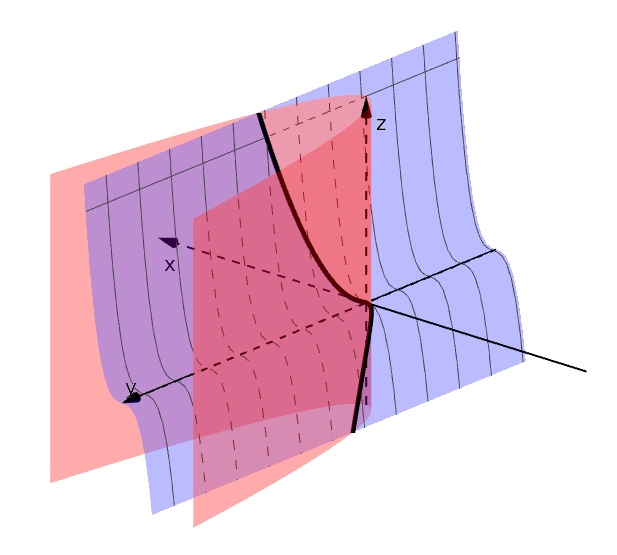
\includegraphics[width=10cm]{cubica-torcida.png}
\end{center}

\begin{proposicion}
  Todo morfismo de conjuntos algebraicos $f\colon X\to Y$ es continuo respecto a
  la topología de Zariski.

  \begin{proof}
    Si $X \subseteq \AA^m (k)$ e $Y \subseteq \AA^n (k)$, entonces $f$ está
    definido por polinomios $f_1, \ldots, f_n \in k [x_1,\ldots,x_m]$. Luego,
    $f$ define un homomorfismo de $k$-álgebras
    \begin{align*}
      f^*\colon k [x'_1,\ldots,x'_n] & \to k [x_1,\ldots,x_m],\\
      x'_i & \mapsto f_i.
    \end{align*}

    Para todo subconjunto cerrado $\mathbf{V} (I) \subseteq Y$ que corresponde a
    un ideal $I \subseteq k [x_1,\ldots,x_n]$ la preimagen es también cerrada:
    \[ f^{-1} (\mathbf{V} (I)) = \{ \underline{a} \in X \mid f (\underline{a}) \in \mathbf{V} (I) \} = \{ \underline{a} \in X \mid g (f (\underline{a})) = f^* (g) (\underline{a}) = 0\text{ para todo }g\in I \} = \mathbf{V} (f^* (I)). \qedhere \]
  \end{proof}
\end{proposicion}

\begin{ejemplo}
  La aplicación $\exp\colon \AA^1 (\CC) \to \AA^1 (\CC)$ no es un morfismo de
  conjuntos algebraicos: para el punto $1 \in \AA^1 (\CC)$ se tiene
  $\exp^{-1} (1) = \{ 2\pi i k \mid k \in \ZZ \}$ que es un subconjunto infinito
  de $\AA^1 (\CC)$ y por ende no es cerrado.
\end{ejemplo}

Para un conjunto algebraico $X \subseteq \AA^n (k)$ los morfismos
$X\to \AA^1 (k)$ forman una $k$-álgebra. En efecto, cada uno de estos morfismos
está definido por un polinomio $f \in k [x_1,\ldots,x_n]$, y los polinomios
pueden ser sumados y multiplicados:
$$(f+g) (\underline{a}) \dfn f (\underline{a}) + g (\underline{a}), \quad (cf) (\underline{a}) \dfn c\,f (\underline{a}), \quad (fg) (\underline{a}) \dfn f (\underline{a}) \, g (\underline{a})$$
para $f,g \in k [x_1,\ldots,x_n]$, $c \in k$, $\underline{a}\in X$.

Dos diferentes polinomios $f,g \in k [x_1,\ldots,x_n]$ definen la misma
aplicación sobre $X$ si y solo si ${f (\underline{a}) = g (\underline{a})}$ para
todo $\underline{a}\in X$; es decir, si y solo si $f-g \in \mathbf{I} (X)$. Se
sigue que hay un isomorfismo natural de $k$-álgebras
$$\Mor (X, \AA^1 (k)) \isom k[x_1,\ldots,x_n]/\mathbf{I} (X).$$

\begin{definicion}
  Para un conjunto algebraico $X \subseteq \AA^n (k)$ la $k$-álgebra
  $$\Gamma (X) \dfn \Mor (X, \AA^1 (k)) \isom k[x_1,\ldots,x_n]/\mathbf{I} (X)$$
  se llama el \term{álgebra de las funciones polinomiales sobre $X$}, o también
  el \term{anillo de coordenadas de $X$}.
\end{definicion}

\begin{ejercicio}
  Demuestre que si $X \subset \AA^n (k)$ es un conjunto finito, entonces
  $$\dim_k \Gamma (X) = |X|.$$
\end{ejercicio}

\begin{proposicion}
  Para cualquier conjunto algebraico $X$ la $k$-álgebra $\Gamma (X)$ es
  finitamente generada y reducida.

  \begin{proof}
    Recordemos que $A$ es una \term{$k$-álgebra finitamente generada} si y solo
    si $A \isom k [x_1,\ldots,x_n]/I$ para algún $n$ y algún ideal
    $I \subseteq k [x_1,\ldots,x_n]$.

    Un anillo $A$ es \term{reducido} si este no tiene nilpotentes no triviales:
    si $f^n = 0$ para algún $f \in A$ y $n = 1,2,3,\ldots$, entonces $f = 0$.
    La $k$-álgebra $\Gamma (X) \isom k [x_1,\ldots,x_n]/\mathbf{I} (X)$ es
    reducida, puesto que el ideal $\mathbf{I} (X)$ es radical.
  \end{proof}
\end{proposicion}

Se ve que un morfismo de conjuntos algebraicos $f\colon X\to Y$ induce
un homomorfismo de $k$-álgebras
\begin{align*}
  f^*\colon \Gamma (Y) & \to \Gamma (X),\\
  (Y\xrightarrow{\phi} \AA^1 (k)) & \mapsto (X\xrightarrow{f} Y\xrightarrow{\phi} \AA^1 (k)),
\end{align*}
así que se trata de un funtor contravariante entre los conjuntos algebraicos
sobre $k$ y $k$-álgebras finitamente generadas reducidas:
$$(\categ{conjuntos algebraicos sobre }k)^\mathrm{op} \to k\categ{-álgebras finitamente generadas reducidas}.$$

\begin{proposicion}
  \label{prop:Gamma-fielmente-pleno}
  El funtor $\Gamma$ es fielmente pleno: para cualesquiera
  $X \subseteq \AA^m (k)$, $Y \subseteq \AA^n (k)$ la aplicación
  \begin{align*}
    \Mor (X,Y) & \xrightarrow{\isom} \Hom (\Gamma (Y), \Gamma (X)),\\
    f & \mapsto f^*
  \end{align*}
  es una biyección entre los morfismos $X\to Y$ y homomorfismos de $k$-álgebras
  $\Gamma (Y) \to \Gamma (X)$.

  \begin{proof}
    Podemos definir una aplicación inversa. Todo homomorfismo de $k$-álgebras
    $\phi\colon \Gamma (Y) \to \Gamma (X)$ puede ser levantado a un homomorfismo
    $\widetilde{\phi}\colon k [x'_1, \ldots, x'_n] \to k [x_1,\ldots,x_m]$:

    \[ \begin{tikzcd}
        k [x'_1, \ldots, x'_n]\ar[->>]{d} \ar[dashed]{r}{\widetilde{\phi}} & k [x_1, \ldots, x_m] \ar[->>]{d} \\
        \Gamma (Y) \ar{r}{\phi} & \Gamma (X)
      \end{tikzcd} \]

    Este $\widetilde{\phi}$ define un morfismo $f\colon X\to Y$ mediante
    $$f (\underline{x}) \dfn (\widetilde{\phi} (x'_1) (\underline{x}), \ldots, \widetilde{\phi} (x'_n) (\underline{x})).$$
    Notamos que diferentes levantamientos de $\phi$ a $\widetilde{\phi}$ definen
    el mismo morfismo $f$. La aplicación $\phi \mapsto f$ es inversa a
    $f \mapsto f^*$.
  \end{proof}
\end{proposicion}

\begin{comentario}
  En general, $\Gamma$ \emph{no es} una equivalencia de categorías: este funtor
  no es esencialmente sobreyectivo. Por ejemplo, si $k = \RR$, entonces
  $\CC \isom \RR [X] / (X^2+1)$ es una $\RR$-álgebra finitamente generada
  reducida. Sin embargo, si $X$ es un conjunto algebraico sobre $\RR$, entonces
  un morfismo $f\colon X \to \AA^1 (\RR)$ no puede cumplir $f^2 = -1$, mientras
  que en $\CC$ hay la unidad imaginaria con esta propiedad.
\end{comentario}

\begin{ejercicio}
  Demuestre que si $k$ es un cuerpo algebraicamente cerrado y $\fchar k \ne 2$,
  entonces la hipérbola $\mathbf{V} (xy - 1)$ y la parábola
  $\mathbf{V} (y - x^2)$ son isomorfas. ¿Qué sucede si $\fchar k = 2$?
\end{ejercicio}

\begin{ejercicio}
  Sea $k = \overline{\FF_p}$, la cerradura algebraica de un cuerpo finito
  $\FF_q$. Demuestre que la aplicación
  $$F\colon (x_1,\ldots,x_n) \mapsto (x_1^p, \ldots, x_n^p)$$
  es un morfismo biyectivo
  $\AA^n (\overline{\FF_p}) \to \AA^n (\overline{\FF_p})$, pero no es un
  isomorfismo.
\end{ejercicio}

\begin{ejercicio}
  Sea $k$ un cuerpo algebraicamente cerrado.

  \begin{enumerate}
  \item[a)] Para $\fchar k \ne 2$ consideremos los siguientes conjuntos
    algebraicos en $\AA^2 (k)$:
    $$Z_1 \dfn \mathbf{V} (u\,(t - 1) - 1), \quad Z_2 \dfn \mathbf{V} (y^2 - x^2 (x + 1)).$$
    Demuestre que el morfismo $Z_1 \to Z_2$,
    $(t, u) \mapsto (t^2 - 1, t\,(t^2 - 1))$ es biyectivo, pero no es un
    isomorfismo.
    Demuestre que en general, $Z_1 \not\isom Z_2$.

  \item[b)] Demuestre que el morfismo
    $\AA^1 (k) \to \mathbf{V} (y^2 - x^3) \subset \AA^2 (k)$,
    $t \mapsto (t^2, t^3)$ es biyectivo, pero no es un isomorfismo.
    Demuestre que en general, $\AA^1 (k) \not\isom \mathbf{V} (y^2 - x^3)$.
  \end{enumerate}

  \noindent Sugerencia: demuestre que $\Gamma (Z_1) \not\isom \Gamma (Z_2)$ y
  $\Gamma (\mathbf{V} (y^2 - x^3)) \not\isom k[t]$.
\end{ejercicio}

\subsection{Teorema de los ceros}

En esta sección vamos a recordar brevemente el teorema de los ceros.

\begin{definicion}
  Se dice que $A$ es un \term{anillo de Jacobson} si todo ideal primo en $A$ es
  una intersección de ideales maximales. En otras palabras, para todo
  $\mathfrak{p} \in \Spec A$ se tiene
  $$\mathfrak{p} = \bigcap_{\substack{ \mathfrak{m} \in \Specm A \\ \mathfrak{m} \supseteq \mathfrak{p}}} \mathfrak{m}.$$
\end{definicion}

\begin{ejemplo}
  Todo cuerpo es trivialmente un anillo de Jacobson: su único ideal propio es
  $(0)$.
\end{ejemplo}

\begin{ejemplo}
  Si $A$ es un dominio de ideales principales, entonces los ideales primos en
  $A$ son de la forma $(0)$ o $(p)$, donde $p \in A$ es primo. Todo ideal primo
  no nulo es maximal. Ahora si se cumple
  $$(0) = \bigcap_{p \in A\text{ primo}} (p),$$
  entonces $A$ es un anillo de Jacobson. Esto sucede si y solamente si en $A$
  hay un número infinito de primos. Por ejemplo, $\ZZ$ y el anillo de polinomios
  en una variable $k [x]$ son anillos de Jacobson.
\end{ejemplo}

El resultado principal, que no vamos a probar aquí\footnote{Lo probamos en el
  curso de álgebra conmutativa.}, es el siguiente.

\begin{teorema}
  Sea $R$ un anillo de Jacobson y $A$ una $R$-álgebra finitamente
  generada. Entonces,

  \begin{enumerate}
  \item[1)] $A$ es también un anillo de Jacobson;

  \item[2)] si $\mathfrak{m} \subset A$ es un ideal maximal, entonces
    $R \cap \mathfrak{m}$ es un ideal maximal en $R$ y el cuerpo
    $A/\mathfrak{m}$ es una extensión finita de $R/(R\cap \mathfrak{m})$.
  \end{enumerate}
\end{teorema}

\begin{corolario}
  Si $A$ es una $k$-álgebra finitamente generada y $\mathfrak{m} \subset A$ es
  un ideal maximal, entonces $A/\mathfrak{m}$ es una extensión finita de $k$.
  En particular, si $k$ es un cuerpo algebraicamente cerrado, entonces
  $A/\mathfrak{m} \isom k$ para todo ideal maximal $\mathfrak{m} \subset A$.
\end{corolario}

\begin{corolario}
  \label{cor:funtorialidad-de-Specm-para-alg-fg}
  Sea $k$ un cuerpo y $\phi\colon A\to B$ un homomorfismo de $k$-álgebras
  finitamente generadas. Si $\mathfrak{m} \subset B$ es un ideal maximal,
  entonces $\phi^{-1} (\mathfrak{m}) \subset A$ es también un ideal maximal.

  \begin{proof}
    El homomorfismo inducido
    $A/\phi^{-1} (\mathfrak{m}) \hookrightarrow B/\mathfrak{m}$ nos permite
    identificar $A/\phi^{-1} (\mathfrak{m})$ con un subanillo del cuerpo
    $B/\mathfrak{m}$. Tenemos entonces
    $$k \subseteq A/\phi^{-1} (\mathfrak{m}) \subseteq B/\mathfrak{m},$$
    donde $B/\mathfrak{m}$ es una extensión finita de $k$. Esto implica que
    $A/\phi^{-1} (\mathfrak{m})$ es un cuerpo, gracias al lema de abajo.
  \end{proof}
\end{corolario}

\begin{lema}
  \label{lema:subalgebra-en-extension-algebraica}
  Sea $L/k$ una extensión algebraica de cuerpos. Entonces, toda $k$-subálgebra
  $A \subseteq L$ es también un cuerpo.

  \begin{proof}
    Todo elemento no nulo $f \in A \subseteq L$ es algebraico sobre $k$, así que
    hay una relación algebraica no trivial
    $$a_n\,f^n + a_{n-1}\,f^{n-1} + \cdots + a_1\,f + a_0 = 0$$
    para algunos $a_0,a_1,\ldots,a_n \in k$, donde sin pérdida de generalidad
    $a_0 \ne 0$. Luego,
    $$a_0 = -f\,(a_n\,f^{n-1} + a_{n-1}\,f^{n-2} + \cdots + a_1),$$
    así que
    $$f^{-1} = -a_0^{-1}\,(a_n\,f^{n-1} + a_{n-1}\,f^{n-2} + \cdots + a_1),$$
    y $f$ es invertible en $A$.
  \end{proof}
\end{lema}

Gracias al corolario \ref{cor:funtorialidad-de-Specm-para-alg-fg}, el espectro
maximal nos da un funtor contravariante
$$(k\categ{-álgebras finitamente generadas})^\mathrm{op} \to \categ{conjuntos}.$$
A saber, un homomorfismo $\phi\colon A\to B$ induce de manera funtorial una
aplicación
\begin{align*}
  \phi^*\colon \Specm B & \to \Specm A,\\
  \mathfrak{m} & \mapsto \phi^{-1} (\mathfrak{m}).
\end{align*}

\begin{comentario}
  En general, la preimagen de un ideal maximal es un ideal primo, pero no
  necesariamente maximal. Considere por ejemplo la inclusión
  $\ZZ \hookrightarrow \QQ$ y el ideal maximal $(0) \subset \QQ$. Por este
  motivo en general hay que trabajar con el espectro $\Spec A$ y no solamente
  con el espectro maximal $\Specm A$.
\end{comentario}

\begin{corolario}
  Sea $k$ un cuerpo algebraicamente cerrado.

  \begin{enumerate}
  \item[1)] Todo ideal maximal en $k [x_1,\ldots,x_n]$ es de la forma
    $\mathfrak{m}_{\underline{a}} = (x_1 - a_1, \ldots, x_n - a_n)$ para algún
    $\underline{x} \in \AA^n (k)$, lo que nos da una biyección natural
    \begin{align*}
      \AA^n (k) & \isom \Specm k [x_1,\ldots,x_n],\\
      \underline{a} & \mapsto \mathfrak{m}_{\underline{a}},\\
      \mathbf{V} (\mathfrak{m}) & \mapsfrom \mathfrak{m}.
    \end{align*}

  \item[2)] Para cualquier conjunto algebraico $X \subseteq \AA^n (k)$ existe
    una biyección natural
    $$X \isom \Specm \Gamma (X).$$
  \end{enumerate}

  \begin{proof}
    En la parte 1), ya hemos notado que para todo punto
    $\underline{a} \in \AA^n (k)$ se cumple
    $\mathbf{V} (\mathfrak{m}_{\underline{a}}) = \underline{a}$. Esto no
    requiere que el cuerpo base $k$ sea algebraicamente cerrado. Ahora para un
    ideal maximal $\mathfrak{m} \subset k [x_1,\ldots,x_n]$ podemos cpnsiderar
    el homomorfismo canónico
    $$\phi\colon k [x_1,\ldots,x_n] \epi k [x_1,\ldots,x_n]/\mathfrak{m} \xrightarrow{\isom} k.$$
    Aquí la última flecha es un isomorfismo,
    \emph{dado que $k$ es algebraicamente cerrado}. Denotemos por $a_i \in k$
    la imagen de $x_i$. Para $\underline{a} = (a_1,\ldots,a_n)$ tenemos
    $\mathfrak{m}_{\underline{a}} \subseteq \ker \phi = \mathfrak{m}$. Luego,
    por la maximalidad de $\mathfrak{m}_{\underline{a}}$, podemos concluir que
    $\mathfrak{m} = \mathfrak{m}_{\underline{a}}$.

    \iffalse
    La naturalidad de la biyección quiere decir lo siquiente: sea
    $f\colon \AA^m (k)\to \AA^n (k)$ un morfismo definido por
    $f_1,\ldots,f_n \in k [x_1,\ldots,x_m]$. A este morfismo corresponde el
    homomorfismo de álgebras
    \begin{align*}
      f^*\colon k [x'_1,\ldots,x'_n] & \to k [x_1,\ldots,x_m],\\
      x'_i & \mapsto f_i
    \end{align*}
    y luego una aplicación entre los espectros maximales
    \begin{align*}
      \Specm k [x_1,\ldots,x_m] & \to \Specm k [x'_1,\ldots,x'_n],\\
      \mathfrak{m}_{\underline{a}} & \mapsto f^{*-1} (\mathfrak{m}_{\underline{a}}).
    \end{align*}

    Calculamos que
    \begin{multline*}
      f^* (\mathfrak{m}_{f(\underline{a})}) = f^* (x_1' - f_1 (\underline{a}), \ldots, x'_n - f_n (\underline{a})) = (f_1 - f_1 (\underline{a}), \ldots, f_n - f_n (\underline{a})) \\
      = (f_1 (\underline{x}-\underline{a}), \ldots, f_n (\underline{x} - \underline{a})) \subseteq (x_1 - a_1, \ldots, x_m - a_m) = \mathfrak{m}_{\underline{a}}.
    \end{multline*}
    Luego, $\mathfrak{m}_{f (\underline{a})} \subseteq \mapsto f^{*-1} (\mathfrak{m}_{\underline{a}})$, lo que nos permite concluir que $f^{*-1} (\mathfrak{m}_{\underline{a}}) = \mathfrak{m}_{f (\underline{a})}$. Entonces, el diagrama
    $$\begin{tikzcd}
      \Specm k [x_1,\ldots,x_m] \ar{r}{\isom}\ar{d}[swap]{f_*} & \AA^m\ar{d}{f} \\
      \Specm k [x'_1,\ldots,x'_n] \ar{r}{\isom} & \AA^n
    \end{tikzcd}$$
    conmuta.
    \fi

    Ahora si $X \subseteq \AA^n (k)$ es un conjunto algebraico, entonces
    $\underline{a}\in X$ si y solo si
    $\mathbf{I} (X) \subseteq \mathfrak{m}_{\underline{a}}$. Tales ideales
    maximales corresponden a los ideales maximales en
    $k [x_1,\ldots,x_n]/\mathbf{I}(X) \isom \Gamma (X)$. Esto nos da
    la biyección en la parte 2).


    Dejo al lector verificar la naturalidad.
  \end{proof}
\end{corolario}

Los ideales $\mathfrak{m}_{\underline{a}} \dfn (x_1-a_1, \ldots, x_n-a_n)$ son
maximales en cualquier caso, pero cuando $k$ no es algebraicamente cerrado,
habrá ideales maximales que no tienen esta forma, como por ejemplo el ideal
$(x^2+1) \subset \RR [x]$.

La biyección $\Specm k [x_1,\ldots,x_n]/\mathbf{I} (X) \isom X$ nos sugiere
considerar la siguiente topología sobre el espectro maximal: los conjuntos
cerrados en $X$ son precisamente $\mathbf{V} (I)$ para los ideales
$I \supseteq \mathbf{I} (X)$, así que podemos declarar que los subconjuntos
cerrados en $\Specm k [x_1,\ldots,x_n]/\mathbf{I} (X)$ son
\begin{equation}
  \label{eqn:topologia-sobre-Specm}
  \mathbf{V} (I) \dfn \{ \mathfrak{m} \in \Specm k [x_1,\ldots,x_n]/\mathbf{I} (X) \mid \mathfrak{m} \supseteq I \} \quad\text{ para }I \subseteq k [x_1,\ldots,x_n]/\mathbf{I} (X).
\end{equation}

\begin{proposicion}
  Sea $I \subseteq k [x_1,\ldots,x_n]$ un ideal.

  \begin{enumerate}
  \item[1)] Se tiene $\sqrt{I} \subseteq \mathbf{IV} (I)$.

  \item[2)] Si $k$ es un cuerpo algebraicamente cerrado, entonces
    $\mathbf{IV} (I) = \sqrt{I}$.
  \end{enumerate}

  \begin{proof}
    La parte 1) puede ser vista directamente sin ningún problema. He aquí una
    explicación complicada: se tiene
    $$\sqrt{I} = \bigcap_{\substack{\mathfrak{p} \in \Spec k [x_1,\ldots,x_n] \\ \mathfrak{p} \supseteq I}} \mathfrak{p} = \bigcap_{\substack{\mathfrak{m} \in \Specm k [x_1,\ldots,x_n] \\ \mathfrak{m} \supseteq I}} \mathfrak{m} \subseteq \bigcap_{\underline{a}\in \mathbf{V} (I)} \mathfrak{m}_{\underline{a}} = \mathbf{IV} (I).$$
    Aquí la segunda igualdad usa el hecho de que $k[x_1,\ldots,x_n]$ es un
    anillo de Jacobson, así que todo ideal primo es una intersección de ideales
    maximales. Si $k$ es algebraicamente cerrado, entonces todos los ideales
    maximales en $k [x_1,\ldots,x_n]$ son de la forma
    $\mathfrak{m}_{\underline{a}}$ para $\underline{a} \in \AA^n (k)$ y la
    inclusión ``$\subseteq$'' de arriba es una igualdad, lo que demuestra la
    parte 2).
  \end{proof}
\end{proposicion}

Si $k$ no es algebraicamente cerrado, entonces el ideal $\mathbf{IV} (I)$ puede
ser más grande que $\sqrt{I}$. Por ejemplo, para $(x^2+1) \subset \RR[x]$ se
tiene $\mathbf{IV} (x^2+1) = \mathbf{I} (\emptyset) = \RR [x]$.

\begin{corolario}
  Si $k$ es un cuerpo algebraicamente cerrado, entonces
  la categoría de conjuntos algebraicos sobre $k$ es antiequivalente
  a la categoría de $k$-álgebras finitamente generadas.

  \begin{proof}
    Hemos probado en \ref{prop:Gamma-fielmente-pleno} que el funtor
    contravariante $\Gamma$ es fielmente pleno. Gracias al teorema de los ceros,
    es también esencialmente sobreyectivo: una $k$-álgebra finitamente generada
    reducida es isomorfa a $k[x_1,\ldots,x_n]/I$ para un ideal radical $I$, y
    luego
    \[ \Gamma (\mathbf{V} (I)) \isom k[x_1,\ldots,x_n]/\mathbf{IV} (I) \isom k[x_1,\ldots,x_n]/I. \qedhere \]
  \end{proof}
\end{corolario}

\begin{ejercicio}
  \label{ejerc:Gamma-X-times-Y}
  Para dos conjuntos algebraicos $X \subseteq \AA^m (k)$ e
  $Y \subseteq \AA^n (k)$, demuestre que $X\times Y \subseteq \AA^{m+n} (k)$ es
  un conjunto algebraico, y es precisamente el producto de $X$ e $Y$ en el
  sentido categórico. Demuestre que si $k$ es un cuerpo algebraicamente cerrado,
  entonces
  $$\Gamma (X\times Y) \isom \Gamma (X)\otimes_k \Gamma (Y).$$
\end{ejercicio}

\begin{teorema}
  Si $k$ es un cuerpo algebraicamente cerrado, entonces existe una biyección

  \[ \begin{tikzcd}
      \{ \text{ideales radicales }I \subseteq k [x_1,\ldots,x_n] \}\ar[shift left=0.25em]{r}{\mathbf{V}} & \{ \text{subconjuntos cerrados }Y \subseteq \AA^n (k) \}\ar[shift left=0.25em]{l}{\mathbf{I}} \\
      \Specm k [x_1,\ldots,x_n]\ar[shift left=0.25em]{r}{\mathbf{V}}\ar[hookrightarrow]{u} & \{ \text{puntos }\underline{a}\in \AA^n (k) \}\ar[shift left=0.25em]{l}{\mathbf{I}}\ar[hookrightarrow]{u}
    \end{tikzcd} \]

  \begin{proof}
    Si $Y \subseteq \AA^n (k)$ es un subconjunto cerrado, entonces
    $$\mathbf{VI} (Y) = \overline{Y} = Y.$$
    Esto se cumple para cualquier $k$, no necesariamente algebraicamente
    cerrado. Ahora si $k$ es algebraicamente cerrado e
    $I \subseteq k [x_1,\ldots,x_n]$ es un ideal radical, entonces
    \[ \mathbf{IV} (I) = \sqrt{I} = I. \qedhere \]
  \end{proof}
\end{teorema}

% % % % % % % % % % % % % % % % % % % % % % % % % % % % % %

\section{Ideales primos y componentes irreducibles}

Recordemos un par de definiciones de topología general.

\begin{definicion}
  Se dice que un espacio topológico $X$ es \term{irreducible} si

  \begin{enumerate}
  \item[1)] $X$ no es vacío;

  \item[2)] $X$ no puede ser representado como una unión $Z_1 \cup Z_2$ donde
    $Z_1,Z_2$ son conjuntos cerrados propios.
  \end{enumerate}

  Un subconjunto $Z \subseteq X$ es \term{irreducible} si es irreducible como un
  espacio con la topología inducida.
\end{definicion}

He aquí otra noción relacionada.

\begin{definicion}
  Se dice que un espacio topológico $X$ es \term{conexo} si

  \begin{enumerate}
  \item[1)] $X$ no es vacío;

  \item[2)] $X$ no puede ser representado como una unión $Z_1 \cup Z_2$ donde
    $Z_1,Z_2$ son conjuntos cerrados propios y $Z_1 \cap Z_2 = \emptyset$.
  \end{enumerate}
  (Notamos que en 2) los conjuntos $Z_1$ y $Z_2$ son también abiertos.)
\end{definicion}

En particular, todo espacio irreducible es necesariamente conexo. Sin embargo,
la irreducibilidad es una propiedad mucho más fuerte.

\begin{proposicion}
  Las siguientes condiciones son equivalentes.

  \begin{enumerate}
  \item[1)] $X$ es irreducible.

  \item[2)] Si $U,V\subseteq X$ son subconjuntos abiertos no vacíos, entonces
    $U\cap V \ne \emptyset$.

  \item[3)] Todo subconjunto abierto no vacío $U \subseteq X$ es denso: se tiene
    $\overline{U} = X$.

  \item[4)] Todo subconjunto abierto no vacío $U \subseteq X$ es conexo.

  \item[5)] Todo subconjunto abierto no vacío $U \subseteq X$ es irreducible.
\end{enumerate}

\begin{proof}
  Ejercicio para el lector.
\end{proof}

\iffalse
\begin{proof}
  \noindent 1)~$\Leftrightarrow$~2). Si para dos abiertos no vacíos
  $U,V \subseteq X$ se tiene $U\cap V = \emptyset$, entonces $U^c \cup V^c = X$,
  donde $U^c$ y $V^c$ son subconjuntos propios cerrados, lo que demuestra que
  $X$ es reducible. Viceversa, si $X = Z_1 \cup Z_2$ donde $Z_1$ y $Z_2$ son
  subconjuntos propios cerrados, entonces $Z_1^c \cup Z_2^c = \emptyset$, donde
  $Z_1^c$ y $Z_2^c$ son subconjuntos abiertos no vacíos.

  \noindent 2)~$\Leftrightarrow$~3). Asumamos que $U\cap V \ne \emptyset$ para
  cualesquiera $U,V\subseteq X$ abiertos no vacíos. Sea $Z \subseteq X$ un
  cerrado tal que $U \subseteq Z \subseteq X$. Si $Z \ne X$, entonces $Z^c$ es
  un abierto no vacío. Pero necesariamente $U \cap Z^c = \emptyset$, así que
  necesariamente $Z = X$. Viceversa, asumamos que $\overline{U} = X$ para todo
  abierto no vacío $U \subseteq X$. Sea $V \subseteq X$ otro abierto no
  vacío. Asumamos que $U\cap V = \emptyset$. Entonces, $U \subseteq V^c$, pero
  esto implicaría $V^c = X$ y $V = \emptyset$. Entonces,
  $U\cap V \ne \emptyset$.

  \noindent 2)~$\Leftrightarrow$~4). Si para dos abiertos no vacíos
  $U,V \subseteq X$ se tiene $U\cap V = \emptyset$, entonces $U\cup V$ es un
  subconjunto abierto disconexo. Esto demuestra que 4) implica 2). Viceversa, si
  $U \subseteq X$ es un abierto disconexo, entonces $U = V_1 \cup V_2$ para dos
  abiertos no vacíos tales que $V_1\cap V_2 = \emptyset$.

  La implicación 5)~$\Leftrightarrow$~1) es obvia. Para terminar la prueba,
  tenemos que deducir 5) de alguna de las condiciones anteriores. Asumamos que
  $X$ es irreducible. Sea $U \subseteq X$ un abierto no vacío reducible. Esto
  significa que existen dos conjuntos cerrados $Z_1, Z_2 \subseteq X$ tales que
  $U = (U\cap Z_1) \cup (U\cap Z_2)$ y $U\cap Z_1 \ne U$, $U\cap Z_2 \ne
  U$. Ahora la cerradura de $U$ en $X$ satisface
  $$\overline{U} = \overline{(U\cap Z_1) \cup (U\cap Z_2)} = \overline{(U\cap Z_1)} \cup \overline{(U\cap Z_2)} \subseteq Z_1 \cup Z_2.$$
  Si $Z_1 \cup Z_2 = X$, esto contradice la irreducibilidad de $X$. Si
  $Z_1\cup Z_2 \ne X$, esto contradice la condición 3).
\end{proof}
\fi
\end{proposicion}

\begin{comentario}
  Ya que en un espacio irreducible $U \cap V \ne \emptyset$ para cualesquiera
  $U,V \subseteq X$ abiertos no vacíos, el axioma de Hausdorff nunca se cumple,
  salvo el caso trivial cuando $X$ consiste en un punto. Por esto el concepto
  de irreducibilidad no se ve mucho en la geometría habitual.
\end{comentario}

\begin{proposicion}
  Sea $X$ un espacio topológico. Un subconjunto $Y \subseteq X$ es irreducible
  si y solo si su cerradura $\overline{Y}$ es irreducible.

  \begin{proof}
    Asumamos que $\overline{Y}$ es irreducible. En particular,
    $\overline{Y} \ne \emptyset$ y por lo tanto $Y \ne \emptyset$. Supongamos
    que $Z_1, Z_2 \subseteq X$ son dos conjuntos cerrados tales que
    $Y = (Y\cap Z_1) \cup (Y\cap Z_2)$. Luego, tomando las cerraduras en $X$, se
    obtiene
    $$\overline{Y} = \overline{(Y\cap Z_1)} \cup \overline{(Y\cap Z_2)}.$$
    Por la irreducibilidad de $\overline{Y}$, tenemos
    $$Y \subseteq \overline{Y} = \overline{Y\cap Z_1} \subseteq Z_1\quad\text{o}\quad Y \subseteq \overline{Y} = \overline{Y\cap Z_2} \subseteq Z_2,$$
    y luego
    $$Y \subseteq Y\cap Z_1\quad\text{o}\quad Y \subseteq Y\cap Z_2.$$
    Esto significa que $Y$ es irreducible.

    Ahora asumamos que $Y$ es irreducible y $\overline{Y} = Z_1 \cup Z_2$, donde
    $Z_1, Z_2$ son cerrados en $\overline{Y}$. Luego,
    $$Y = (Y\cap Z_1) \cup (Y\cap Z_1),$$
    y por la irreducibilidad de $Y$ se tiene $Y = Y\cap Z_1$ o $Y = Y\cap
    Z_2$. Entonces, $\overline{Y} \subseteq Z_1$ o $\overline{Y} \subseteq Z_2$.
  \end{proof}
\end{proposicion}

\iffalse
\begin{proposicion}
  Para todo subconjunto abierto $U \subseteq X$ existe una biyección

  \[ \begin{tikzcd}[column sep=5em]
      \{ Y\subseteq U\text{ irreducibles, cerrados en }U \} \ar[shift left=0.25em]{r}{Y \mapsto \overline{Y}} & \{ \text{irreducibles, cerrados }Z\subseteq X, ~ Z\cap U \ne \emptyset \}\ar[shift left=0.25em]{l}{Z\cap U \mapsfrom Z}
    \end{tikzcd} \]

  \begin{proof}
    Verifiquemos que las aplicaciones son bien definidas. Si $Y \subseteq U$ es
    irreducible, entonces, como vimos arriba, su cerradura $\overline{Y}$ en $X$
    es también irreducible. Ahora si $Z \subseteq X$ es un conjunto cerrado
    irreducible tal que $Z\cap U \ne \emptyset$, entonces $Z\cap U$ es cerrado
    en $U$ y es irreducible, siendo abierto en $Z$.

    Ahora para un conjunto irreducible $Y \subseteq U$, cerrado en $U$, tenemos
    $\overline{Y} \cap U = Y$. Viceversa, si $Z \subseteq X$ es irreducible,
    cerrado y $Z\cap U \ne \emptyset$, entonces $Z\cap U$ es abierto en $Z$ y
    por esto $\overline{Z\cap U} = Z$.
  \end{proof}
\end{proposicion}
\fi

\begin{definicion}
  Sea $X$ un espacio topológico. Un subconjunto irreducible de $X$ maximal
  respecto a la inclusión se llama una \term{componente irreducible} de $X$.
\end{definicion}

\begin{proposicion}
  Las componentes irreducibles son cerradas.

  \begin{proof}
    Si $Y \subseteq X$ es irreducible, entonces $\overline{Y} \supseteq Y$ es
    también irreducible. Por maximalidad de $Y$, se tiene $\overline{Y} = Y$.
  \end{proof}
\end{proposicion}

\begin{proposicion}
  Sea $X$ un espacio topológico. Todo subconjunto irreducible de $X$ está
  contenido en una componente irreducible. En particular, todo punto de $X$ está
  contenido en alguna componente irreducible y $X$ es la unión\footnote{¡No
    necesariamente disjunta! No confundir con la situación con componentes
    \emph{conexas} que son disjuntas.} de sus componentes irreducibles.

  \begin{proof}
    Se sigue del lema de Zorn. Sea $Z \subseteq X$ un subconjunto
    irreducible. Para toda cadena
    $$Z \subseteq Z_1 \subseteq Z_2 \subseteq Z_3 \subseteq \cdots \subset X$$
    de subconjuntos irreducibles la unión $\bigcup_i Z_i$ es también
    irreducible. Entonces, existe un conjunto irreducible maximal que contiene a
    $Z$.
  \end{proof}
\end{proposicion}

\begin{teorema}
  Sea $k$ un cuerpo.

  \begin{enumerate}
  \item[1)] Si $Z \subseteq \AA^n (k)$ es un subconjunto cerrado irreducible,
    entonces el ideal $\mathbf{I} (Z)$ es primo.

  \item[2)] Si $k$ es algebraicamente cerrado y
    $\mathfrak{p} \subset k [x_1,\ldots,x_n]$ es un ideal primo, entonces
    $\mathbf{V} (\mathfrak{p}) \subseteq \AA^n (k)$ es irreducible. En
    particular, $\AA^n (k) = \mathbf{V} (0)$ es irreducible.
  \end{enumerate}

  \begin{proof}
    Sea $Z = \mathbf{V} (I)$ para algún ideal $I \subset k
    [x_1,\ldots,x_n]$. Primero, notamos que $\mathbf{V} (I) \ne \emptyset$
    implica que $\mathbf{IV} (I) \ne k [x_1,\ldots,x_n]$. Asumamos que
    $\mathbf{V} (I)$ es irreducible y $fg\in \mathbf{IV} (I)$. Luego,
    $$\mathbf{V} (I) = \mathbf{VIV} (I) \subseteq \mathbf{V} (fg) = \mathbf{V} (f) \cup \mathbf{V} (g)$$
    y por ende
    $$\mathbf{V} (I) = (\mathbf{V} (I) \cap \mathbf{V} (f)) \cup (\mathbf{V} (I) \cap \mathbf{V} (g)).$$
    Por la irreducibilidad se tiene $\mathbf{V} (I) \subseteq \mathbf{V} (f)$ o
    $\mathbf{V} (I) \subseteq \mathbf{V} (g)$. Por ejemplo, en el primer caso,
    $$f \in \sqrt{(f)} \subseteq \mathbf{IV} (f) \subseteq \mathbf{IV} (I).$$
    De la misma manera, en el segundo caso $g \in \mathbf{IV} (I)$. Esto
    demuestra que el ideal $\mathbf{IV} (I)$ es primo.

    Ahora asumamos que $k$ es algebraicamente cerrado. Sea $\mathfrak{p}$ un
    ideal primo. Supongamos que
    $$\mathbf{V} (\mathfrak{p}) = \mathbf{V} (I) \cup \mathbf{V} (J) = \mathbf{V} (IJ),$$
    donde $\mathbf{V} (I)$ y $\mathbf{V} (J)$ son dos subconjuntos cerrados de
    $\mathbf{V} (\mathfrak{p})$. Luego, aplicando la operación $\mathbf{I}$, se
    obtiene
    $$\mathfrak{p} = \mathbf{IV} (\mathfrak{p}) = \mathbf{IV} (IJ) = \sqrt{IJ} \supseteq IJ.$$
    Dado que $\mathfrak{p}$ es primo, esto implica $I \subseteq \mathfrak{p}$ o
    $J \subseteq \mathfrak{p}$, y por lo tanto
    $\mathbf{V} (\mathfrak{p}) = \mathbf{V} (I)$ o
    $\mathbf{V} (\mathfrak{p}) = \mathbf{V} (J)$.
  \end{proof}
\end{teorema}

Cuando el cuerpo base $k$ no es algebraicamente cerrado, para un ideal primo
$\mathfrak{p} \subset k [x_1,\ldots,x_n]$ el conjunto correspondiente
$\mathbf{V} (\mathfrak{p})$ no es necesariamente irreducible. He aquí algunos
ejemplos.

\begin{enumerate}
\item[1)] El conjunto $\mathbf{V} (\mathfrak{p})$ puede ser vacío, como en el
  caso de $(x^2+1) \subset \RR[x]$.

\item[2)] El polinomio $x^2 + y^2\,(y-1)^2$ es irreducible en $\RR [x,y]$, y
  entonces genera un ideal primo, pero
  $$\mathbf{V} (x^2 + y^2\,(y-1)^2) = \{ (0,0), \, (0,1) \}.$$

\item[3)] Si $k = \FF_q$ es un cuerpo finito, al ideal primo
  $(0) \subset \FF_q [x_1,\ldots,x_n]$ corresponde el espacio $\AA^n (\FF_q)$
  que es reducible, siendo la unión de un número finito de puntos.
\end{enumerate}

\begin{corolario}
  Sea $k$ es un cuerpo algebraicamente cerrado.

  \begin{enumerate}
  \item[1)] Existe una biyección natural
    \[ \begin{tikzcd}
        \Spec k [x_1,\ldots,x_n]\ar[shift left=0.25em]{r}{\mathbf{V}} & \{ \text{subconjuntos cerrados irreducibles }X \subseteq \AA^n (k) \}\ar[shift left=0.25em]{l}{\mathbf{I}} \\
        \Specm k [x_1,\ldots,x_n]\ar[shift left=0.25em]{r}{\mathbf{V}}\ar[hookrightarrow]{u} & \{ \text{puntos }\underline{a}\in \AA^n (k) \}\ar[shift left=0.25em]{l}{\mathbf{I}}\ar[hookrightarrow]{u}
      \end{tikzcd} \]

  \item[2)] Para cualquier conjunto algebraico $X \subseteq \AA^n (k)$ existe una biyección natural
    \[ \begin{tikzcd}
        \Spec \Gamma (X)\ar[shift left=0.25em]{r}{\mathbf{V}} & \{ \text{subconjuntos cerrados irreducibles }Y \subseteq X \}\ar[shift left=0.25em]{l}{\mathbf{I}} \\
        \Specm \Gamma (X)\ar[shift left=0.25em]{r}{\mathbf{V}}\ar[hookrightarrow]{u} & \{ \text{puntos }\underline{a}\in X \}\ar[shift left=0.25em]{l}{\mathbf{I}}\ar[hookrightarrow]{u}
      \end{tikzcd} \]
  \end{enumerate}

  \begin{proof}
    Se sigue de las identidades $\mathbf{IV} (\mathfrak{p}) = \mathfrak{p}$ y
    $\mathbf{VI} (X) = X$.
  \end{proof}
\end{corolario}

Si $k$ no es algebraicamente cerrado, entonces diferentes ideales primos pueden
corresponder al mismo subconjunto cerrado irreducible. Por ejemplo, si
$k = \RR$, entonces
$$\mathbf{V} (x,y) = \mathbf{V} (x^2+y^2) = \{ (0,0) \}.$$

\begin{digresion}
  \label{digresion:topologia-sobre-Spec}
  La topología de \eqnref{eqn:topologia-sobre-Specm} motiva la siguiente
  definición general: para cualquier anillo conmutativo $A$ los subconjuntos
  cerrados de $\Spec A$ son
  $$\mathbf{V} (I) \dfn \{ \mathfrak{p} \in \Spec A \mid \mathfrak{p} \supseteq I \} \quad\text{ para ideales }I \subseteq A.$$
  Esto define una topología sobre $\Spec A$ que también se conoce como la
  \term{topología de Zariski}. Este es el punto de partida en la definición del
  \term{esquema afín}. Aquí se considera el espectro y no solamente el espectro
  maximal porque un homomorfismo $\phi\colon A\to B$ induce una aplicación
  continua
  \begin{align*}
    \phi^*\colon \Spec B & \to \Spec A,\\
    \mathfrak{p} & \mapsto \phi^{-1} (\mathfrak{p}).
  \end{align*}
  Para los anillos conmutativos en general, la preimagen de un ideal maximal no
  tiene por qué ser maximal.
\end{digresion}

\begin{corolario}
  Sea $k$ es un cuerpo algebraicamente cerrado. Las componentes irreducibles de
  un conjunto algebraico $\mathbf{V} (I)$ corresponden a los ideales primos
  \term{minimales} que contienen al ideal $I$.

  \begin{proof}
    Las operaciones $\mathbf{I}$ y $\mathbf{V}$ invierten las inclusiones,
    así que los conjuntos irreducibles maximales
    $\mathbf{V} (\mathfrak{p}) \subseteq \mathbf{V} (I)$ corresponden a
    los ideales primos minimales
    $\mathfrak{p} = \mathbf{IV} (\mathfrak{p}) \supseteq \mathbf{IV} (I) =
    \sqrt{I} \supseteq I$.
  \end{proof}
\end{corolario}

\begin{ejemplo}
  El conjunto algebraico $\mathbf{V} (xy) \subset \AA^2 (k)$ es reducible:
  el ideal $\mathbf{IV} (xy) = (xy)$ no es primo, sino es la intersección de
  dos ideales primos $(x)$ e $(y)$.
  Tenemos $\mathbf{V} (xy) = \mathbf{V} (x) \cup \mathbf{V} (y)$.
  Los ideales $(x)$ e $(y)$ son minimales en el siguiente sentido:
  por ejemplo, si $(xy) \subseteq \mathfrak{p} \subseteq (x)$ para un ideal
  primo $\mathfrak{p}$, entonces $\mathfrak{p} = (x)$.
\end{ejemplo}

\begin{ejercicio}
  Sea $k$ es un cuerpo algebraicamente cerrado. Encuentre las componentes
  irreducibles de los siguientes conjuntos algebraicos:
  \begin{enumerate}
  \item[1)] $\mathbf{V} (x\,(x+1), y) \subset \AA^2 (k)$;
  \item[2)] $\mathbf{V} (xz, yz) \subset \AA^3 (k)$;
  \item[3)] $\mathbf{V} (xy^2-x^2\,(x^2-1)) \subset \AA^2 (k)$.
  \end{enumerate}
\end{ejercicio}

\begin{definicion}
  Se dice que un espacio topológico $X$ es \term{noetheriano} si toda cadena
  descendente de subconjuntos cerrados
  $$X \supseteq Z_1 \supseteq Z_2 \supseteq Z_3 \supseteq \cdots$$
  se estabiliza.
\end{definicion}

\begin{lema}
  Si $X$ es un espacio noetheriano, entonces todo subespacio $Y \subseteq X$ es
  noetheriano.

  \begin{proof}
    Sea
    $$Y \supseteq Z_1 \supseteq Z_2 \supseteq Z_3 \supseteq \cdots$$
    una cadena de subespacios cerrados en $Y$. Tomando las cerraduras en $X$ se
    obtiene una cadena
    $$X \supseteq \overline{Z_1} \supseteq \overline{Z_2} \supseteq \overline{Z_3} \supseteq \cdots$$
    que se estabiliza. Ahora $Z_i = Y\cap \overline{Z_i}$.
  \end{proof}
\end{lema}

\begin{proposicion}
  Todo subespacio $X \subseteq \AA^n (k)$ es noetheriano.

  \begin{proof}
    Gracias al lema anterior, bastaría probar que $\AA^n (k)$ es un espacio
    noetheriano. Consideremos una cadena
    $$\AA^n (k) \supseteq \mathbf{V} (I_1) \supseteq \mathbf{V} (I_2) \supseteq \mathbf{V} (I_3) \supseteq \cdots$$
    Esta nos da una cadena de ideales
    $$\mathbf{IV} (I_1) \subseteq \mathbf{IV} (I_2) \subseteq \mathbf{IV} (I_3) \subseteq \cdots \subseteq k [x_1,\ldots,x_n]$$
    que se estabiliza, puesto que $k [x_1,\ldots,x_n]$ es un anillo
    noetheriano. Tenemos entonces
    $$\mathbf{IV} (I_n) = \mathbf{IV} (I_{n+1}) = \mathbf{IV} (I_{n+2}) = \cdots$$
    Luego, dado que $\mathbf{VIV} (I) = \mathbf{V} (I)$,
    \[ \mathbf{V} (I_n) = \mathbf{V} (I_{n+1}) = \mathbf{V} (I_{n+2}) = \cdots \qedhere \]
  \end{proof}
\end{proposicion}

\begin{digresion}
  Si $A$ es un anillo noetheriano, entonces el espacio $\Spec A$ con
  la topología definida en \ref{digresion:topologia-sobre-Spec} es también
  noetheriano. Sin embargo, si $\Spec A$ es noetheriano, entonces $A$ no es
  necesariamente noetheriano, sino cumple la condición de cadenas ascendentes
  \emph{para los ideales radicales}. Por ejemplo,
  $A = k[x_1,x_2,x_3,\ldots]/(x_1^2,x_2^2,x_3^2,\ldots)$ no es noetheriano, pero
  $\Spec A$ consiste en un punto.
\end{digresion}

\begin{proposicion}
  \label{prop:componentes-irreducibles-de-esp-noetheriano}
  Si $X$ es un espacio noetheriano, entonces todo subconjunto cerrado
  $Z \subseteq X$ tiene un número finito de componentes irreducibles.

  \begin{proof}[Demostración (inducción noetheriana)]
    Bastaría probar que todo subconjunto cerrado de $X$ puede ser expresado como
    una unión finita de subconjuntos irreducibles. Asumamos que esto no es
    cierto y sea $\mathcal{S}$ el conjunto de los subconjuntos cerrados de $X$
    que no pueden ser expresados como una unión finita de subconjuntos
    irreducibles. En este caso, usando que $X$ es noetheriano, podemos concluir
    que en $\mathcal{S}$ existe un elemento mínimo $Z$. Este conjunto no es
    irreducible y por ende $Z = Z_1 \cup Z_2$, donde $Z_1$ y $Z_2$ son
    subconjuntos propios cerrados en $Z$. Por la minimalidad,
    $Z_1,Z_2 \notin \mathcal{S}$, y entonces $Z_1$ y $Z_2$ sí se expresan como
    una unión finita de subconjuntos irreducibles. Esto nos lleva a una
    contradicción.
  \end{proof}
\end{proposicion}

\begin{comentario}
  El argumento de arriba puede ser explicado de manera informal pero tal vez más
  clara. Si $Z$ es irreducible, entonces no hay que hacer nada. Sino, se tiene
  $Z = Z_1 \cup Z_2$, donde $Z_1$ y $Z_2$ son subconjuntos propios cerrados de
  $Z$. Ahora el mismo argumento puede ser aplicado a $Z_1$ y
  $Z_2$. Eventualmente este proceso se termina gracias a la noetherianidad del
  espacio. Como resultado se obtiene una expresión
  $$Z = Z_1 \cup \cdots \cup Z_s,$$
  donde $Z_i$ son conjuntos cerrados irreducibles. Quitando los términos
  innecesarios, podemos asumir que la descomposición es minimal en el sentido de
  que $Z_i \not\subseteq Z_j$ para $i \ne j$.

  Tales descomposiciones minimales son únicas. En efecto, asumamos que
  $$Z = Z_1 \cup \cdots \cup Z_s = Z'_1 \cup \cdots \cup Z'_t.$$
  Ahora $Z'_1 \subseteq Z_1 \cup \cdots \cup Z_s$ implica por la irreducibilidad
  de $Z'_1$ que $Z'_1 \subseteq Z_i$ para algún $i$. El mismo argumento aplicado
  a $Z_i$ nos da $Z_i \subseteq Z'_j$ para algún $j$. Ahora por la minimalidad
  de las descomposiciones,
  $$Z'_1 \subseteq Z_i \subseteq Z'_j$$
  implica que $j = 1$ y $Z'_1 = Z_i$. Podemos quitar $Z'_1$ y $Z_i$ y por
  inducción repetir el argumento a los conjuntos de las uniones que nos
  quedan. Esto nos lleva a la conclusión de que $s = t$ y $Z_i = Z'_i$, salvo
  alguna permutación de los índices.
\end{comentario}

\begin{ejercicio}
  Demuestre que $X$ es un espacio Hausdorff noetheriano si y solo si $X$ es
  finito con la topología discreta.
\end{ejercicio}

Ahora si $k$ es un cuerpo algebraicamente cerrado, entonces para todo ideal
$I \subseteq k[x_1,\ldots,x_n]$ la descomposición en componentes irreducibles
$$\mathbf{V} (I) = Z_1 \cup \cdots \cup Z_s$$
nos da la descomposición
$$\sqrt{I} = \mathfrak{p}_1 \cap \cdots \cap \mathfrak{p}_s,$$
donde $\mathfrak{p}_i = \mathbf{I} (Z_i)$ son ideales primos. Además,
$\mathfrak{p}_i\not\subseteq\mathfrak{p}_j$ para $i\ne j$ y estos ideales primos
están definidos de modo único por $\sqrt{I}$. Esta es una versión muy débil de
la \term{descomposición primaria} en álgebra conmutativa que vamos a investigar
en la siguiente sección.

% % % % % % % % % % % % % % % % % % % % % % % % % % % % % %

\section{Descomposiciones primarias}

La descomposición de un conjunto algebraico en componentes irreducibles tiene su
análogo en el mundo de álgebra conmutativa que es la descomposición primaria de
ideales. Sin embargo, la situación algebraica es más sutil. Nuestra exposición
esencialmente sigue \cite[Chapter 4]{Atiyah-Macdonald}.

Para motivar la teoría de esta sección, consideremos un dominio de factorización
única $A$. En este caso todo elemento no nulo $f\in A$ se descompone como
$$f = u\,p_1^{k_1}\cdots p_s^{k_s},$$
donde $u \in A^\times$ es un elemento invertible y $p_1,\ldots,p_s\in A$ son
elementos primos no asociados entre sí. En términos de ideales, esta
descomposición corresponde a
$$(f) = \mathfrak{q}_1\cap \cdots \cap \mathfrak{q}_s,$$
donde $\mathfrak{q}_i = (p_i^{k_i})$. El objetivo de esta sección es generalizar
tales expresiones a ideales $I \subseteq A$ en cualquier anillo noetheriano
$A$. Los ideales $\mathfrak{q}_i$ de arriba son un caso particular de ideales
primarios.

\subsection{Ideales primarios}

\begin{definicion}
  Sea $A$ un anillo conmutativo. Se dice que un ideal $\mathfrak{q} \subset A$
  es \term{primario} si el anillo cociente $A/\mathfrak{q}$ tiene las siguientes
  propiedades:

  \begin{enumerate}
  \item[1)] $A/\mathfrak{q} \ne 0$;

  \item[2)] todo divisor de cero en $A/\mathfrak{q}$ es nilpotente.
  \end{enumerate}
  De modo equivalente, esto quiere decir que
  \begin{enumerate}
  \item[1)] $\mathfrak{q} \ne A$;

  \item[2)] para cualesquiera $f,g\in A$, si $fg \in \mathfrak{q}$, entonces
    $f \in \mathfrak{q}$ o $g \in \sqrt{\mathfrak{q}}$ (es decir,
    $g^r \in \mathfrak{q}$ para algún $r = 1,2,3,\ldots$).
  \end{enumerate}
\end{definicion}

Notamos que todo ideal primo es primario: en la definición de ideal primo
$\mathfrak{p} \subset A$ se pide que el anillo cociente $A/\mathfrak{p}$ sea
un dominio, y la definición de ideal primario impone una condición más débil.

\begin{observacion}
  Para todo homomorfismo $\phi\colon A\to B$, si $\mathfrak{q} \subset B$ es
  un ideal primario, entonces $\phi^{-1} (\mathfrak{q}) \subset A$ es también
  primario.

  \begin{proof}
    Notamos que $\phi$ induce un homomorfismo inyectivo
    ${A/\phi^{-1} (\mathfrak{q}) \hookrightarrow B/\mathfrak{q}}$.
  \end{proof}
\end{observacion}

\begin{observacion}
  Si $\mathfrak{q} \subset A$ es un ideal primario, entonces su radical
  $\sqrt{\mathfrak{q}}$ es el ideal primo más pequeño que contiene
  a $\mathfrak{q}$.

  \begin{proof}
    Recordemos que en general, para cualquier ideal $I \subseteq A$ se cumple
    $$\sqrt{I} = \bigcap_{\substack{\mathfrak{p} \in \Spec A \\ \mathfrak{p} \supseteq I}} \mathfrak{p},$$
    así que sería suficiente comprobar que si $\mathfrak{q} \subset A$ es
    primario, entonces $\sqrt{\mathfrak{q}}$ es primo. Primero, dado que
    $\mathfrak{q} \ne A$, se tiene $\sqrt{\mathfrak{q}} \ne A$. Ahora si
    $fg \in \sqrt{\mathfrak{q}}$, entonces se tiene $(fg)^r \in \mathfrak{q}$
    para algún $r = 1,2,3,\ldots$ Luego, ya que $\mathfrak{q}$ es primario,
    tenemos $f^r \in \mathfrak{q}$ o $g^{rs} \in \mathfrak{q}$ para algún
    $s = 1,2,3,\ldots$ Esto significa que $f \in \sqrt{\mathfrak{q}}$ o
    $g \in \sqrt{\mathfrak{q}}$.
  \end{proof}
\end{observacion}

\begin{definicion}
  Si $\mathfrak{q} \subset A$ es un ideal primario y
  $\sqrt{\mathfrak{q}} = \mathfrak{p}$, entonces se dice que $\mathfrak{q}$ es
  un ideal \term{$\mathfrak{p}$-primario}.
\end{definicion}

\begin{observacion}
  \label{obs:interseccion-de-ideales-p-primarios}
  Si $\mathfrak{q}_1,\ldots,\mathfrak{q}_s \subset A$ son ideales
  $\mathfrak{p}$-primarios, entonces su intersección
  $\mathfrak{q}_1\cap\cdots\cap\mathfrak{q}_s$ es también un ideal
  $\mathfrak{p}$-primario.

  \begin{proof}
    Es fácil verificar a partir de la definición que la intersección de ideales
    primarios $\mathfrak{q}_1 \cap \cdots \cap \mathfrak{q}_s$ es un ideal
    primario si
    $\sqrt{\mathfrak{q}_1} = \cdots = \sqrt{\mathfrak{q}_s}$. Además,
    \[ \sqrt{\mathfrak{q}_1 \cap \cdots \cap \mathfrak{q}_s} = \sqrt{\mathfrak{q}_1} \cap \cdots \cap \sqrt{\mathfrak{q}_s} = \mathfrak{p}. \qedhere \]
  \end{proof}
\end{observacion}

\begin{ejemplo}
  Si $A$ es un dominio de factorización única y $p \in A$ es un elemento primo,
  entonces el ideal principal $\mathfrak{q} = (p^k)$ para $k = 1,2,3,\ldots$ es
  primario.
\end{ejemplo}

\begin{ejemplo}
  Sea $A$ un dominio de ideales principales. En particular, $A$ es un dominio de
  factorización única y todo elemento no nulo y no ivertible $f\in A$ se
  factoriza como
  $$f = u\,p_1^{k_1}\cdots p_s^{k_s},$$
  donde $s \ge 1$, $u \in A^\times$ y $p_1,\ldots,p_s \in A$ son elementos
  primos. Ahora si el ideal $(f)$ es primario, su radical
  $$\sqrt{(f)} = (p_1\cdots p_s)$$
  debe ser un ideal primo, así que necesariamente $s = 1$. Esto nos permite
  concluir que los ideales primarios no nulos en $A$ son precisamente de la
  forma $(p^k) = (p)^k$, donde $p \in A$ es un elemento primo y
  $k = 1,2,3,\ldots$ Además, el ideal nulo $(0)$ es también primario.
\end{ejemplo}

Notamos que en el último ejemplo los ideales primarios no nulos son precisamente
las potencias de ideales maximales. Sin embargo, en general, un ideal primario
no debe ser una potencia de un ideal primo, y viceversa, una potencia de
un ideal primo no es siempre un ideal primario.

\begin{ejemplo}
  En el anillo de polinomios $A \dfn k [x,y]$ consideremos el ideal
  $\mathfrak{q} = (x,y^2)$. Notamos que
  $$A/\mathfrak{q} \isom k [y]/(y^2),$$
  y se ve fácilmente que los divisores de cero en este anillo son de la forma
  $a\,\overline{y}$, donde $a \in k$, y estos son nilpotentes. Se sigue que
  $\mathfrak{q}$ es un ideal primario. Ahora si $\mathfrak{q}$ fuera una
  potencia de algún ideal primo, este ideal sería precisamente su radical:
  $\sqrt{\mathfrak{p}^k} = \mathfrak{p}$. Sin embargo, en este caso el radical
  de $\mathfrak{q}$ es el ideal maximal
  $\mathfrak{p} = \sqrt{\mathfrak{q}} = (x,y)$, y se ve que
  $\mathfrak{p}^2 \subsetneq \mathfrak{q} \subsetneq \mathfrak{p}$. Entonces,
  $\mathfrak{q}$ es un ideal primario que no es una potencia de un ideal primo.
\end{ejemplo}

\begin{ejemplo}
  \label{ejemplo:potencia-de-primo-no-primaria}
  Consideremos el anillo cociente $A \dfn k [x,y,z]/(xy-z^2)$. El ideal
  $\mathfrak{p} \dfn (\overline{x},\overline{z})$ es primo: se tiene
  $A/\mathfrak{p} \isom k [y]$. Ahora
  $\overline{x}\,\overline{y} = \overline{z}^2 \in \mathfrak{p}^2$, pero
  $\overline{x} \notin \mathfrak{p}^2$ e $\overline{y}^r \notin \mathfrak{p}^2$
  para ningún $r = 1,2,3,\ldots$ Esto significa que el ideal $\mathfrak{p}^2$ no
  es primario.
\end{ejemplo}

De hecho, se puede construir un ejemplo parecido en el anillo $k [x,y,z]$.

\begin{ejemplo}[\cite{Northcott-1953}]
  \label{ejemplo:potencia-de-primo-no-primaria-2}
  Para los polinomios
  $$f = y^2 - xz, \quad g = yz - x^3, \quad h = z^2 - x^2y$$
  el ideal
  $$\mathfrak{p} = (f,g,h) \subset k [x,y,z]$$
  es primo, pero $\mathfrak{p}^2$ no es primario.

  Para ver que $\mathfrak{p}$ es primo, consideremos el homomorfismo
  $$\phi\colon k [x,y,z] \to k [t], \quad x \mapsto t^3, y \mapsto t^4, z \mapsto t^5.$$
  Primero, está claro que $f,g,h \in \ker \phi$. Luego, todo polinomio en
  $k [x,y,z]$ puede ser escrito como
  $$x^2\,A (z) + xy\,B (z) + x\,C (z) + y\,D (z) + E (z) + F (x,y,z),$$
  donde $A,B,C,D,E \in k [z]$ y $F (x,y,z) \in (f,g,h)$. La imagen de este
  polinomio respecto a $\phi$ es
  $$t^6\,A (t^5) + t^7\,B (t^5) + t^3\,C (t^5) + t^4\,D (t^5) + E (t^5).$$
  Asumamos que este polinomio es igual a $0$. Tenemos
  $$\sum_i a_i\,t^{5i + 6} + \sum_i b_i\,t^{5i + 7} + \sum_i c_i\,t^{5i + 3} + \sum_i d_i\,t^{5i + 4} + \sum_i e_i\,t^{5i} = 0.$$
  Los números $6,7,3,4,0$ dan diferentes restos módulo $5$, así que entre los
  términos no hay cancelaciones y necesariamente $A=B=C=D=E=0$. Esto demuestra
  que $\ker \phi \subseteq (f,g,h)$. Entonces,
  $$\ker \phi = \mathfrak{p},$$
  y podemos concluir que
  $$k [x,y,z]/\mathfrak{p} \cong k [t^3,t^4,t^5] \subset k [t],$$
  y el ideal $\mathfrak{p}$ es primo.

  Ahora tenemos
  $$g^2 - fh = (x^5 + xy^3 - 3x^2 y z + z^3)\,x \in \mathfrak{p}^2,$$
  pero
  $$x^5 + xy^3 - 3x^2 y z + z^3 \notin \mathfrak{p}^2, \quad x \notin \mathfrak{p} = \sqrt{\mathfrak{p}^2}$$
  ---para verlo, notamos que los polinomios en
  $\mathfrak{p} = (y^2 - xz, \, yz - x^3, \, z^2 - x^2y)$ tienen monomios de
  grado $\ge 2$ y los polinomios en $\mathfrak{p}^2$ tienen monomios de grado
  $\ge 4$. Esto significa que el ideal $\mathfrak{p}^2$ no es primario.
\end{ejemplo}

Lo que es cierto es que las potencias de ideales \emph{maximales} son ideales
primarios.

\begin{proposicion}
  Si para un ideal $I \subset A$ su radical $\sqrt{I}$ es un ideal maximal,
  entonces $I$ es primario. En particular, para cualquier ideal maximal
  $\mathfrak{m} \subset A$ sus potencias $\mathfrak{m}^k$ son ideales primarios.

  \begin{proof}
    Recordemos que los ideales primos en el anillo cociente $A/I$ corresponden a
    los ideales primos $\mathfrak{p} \subset A$ tales que
    $\mathfrak{p} \supseteq I$. La última condición es equivalente a
    $\mathfrak{p} \supseteq \sqrt{I}$. Pero por nuestra hipótesis el ideal
    $\sqrt{I}$ es maximal, y por ende el único ideal primo en $A/I$ es el ideal
    $\sqrt{I}/I$, y es también maximal. Ahora los nilpotentes vienen dados por
    $$N (A/I) = \bigcap_{\mathfrak{p} \in \Spec A/I} \mathfrak{p} = \sqrt{I}/I.$$
    Entonces, los elementos de $A/I$ o son nilpotentes, o bien no pertenecen al
    único ideal maximal $\sqrt{I}/I$, y en este caso son invertibles. Esto nos
    permite concluir que $I$ es un ideal primario.
  \end{proof}
\end{proposicion}

\begin{ejercicio}
  Demuestre que en el anillo $A = \ZZ [x]$ el ideal $\mathfrak{m} \dfn (2,x)$ es
  maximal y el ideal $\mathfrak{q} = (4,x)$ es $\mathfrak{m}$-primario, pero no
  es una potencia de $\mathfrak{m}$.
\end{ejercicio}

\begin{ejercicio}[*]
  Encuentre una caracterización de ideales monomiales primarios. Por ejemplo, el
  ideal principal $(x^2y) \subset k [x,y]$ no es primario, mientras que
  $(x^2,y^2)$ es primario.
\end{ejercicio}

\subsection{Digresión: el ideal cociente $(I : J)$}

Recordemos brevemente la siguiente construcción.

\begin{definicion}
  Para dos ideales $I,J\subseteq A$ el \term{ideal cociente} de $I$ por $J$
  viene dado por
  $$(I : J) \dfn \{ f \in A \mid fJ \subseteq I \}.$$
\end{definicion}

\begin{observacionejerc}
  El ideal cociente $(I : J)$ es un ideal. Además, se cumplen las siguientes
  propiedades:
  \begin{enumerate}
  \item[1)] $I \subseteq (I : J)$;

  \item[2)] si $J_1 \subseteq J_2$, entonces $(I : J_1) \supseteq (I : J_2)$;

  \item[3)] $(\bigcap_i I_i : J) = \bigcap_i (I_i : J)$;

  \item[4)] si $J = (f)$ es un ideal principal, entonces
    $(I : f) = \{ g\in A \mid fg \in I \}$. \qedhere
  \end{enumerate}
\end{observacionejerc}

\begin{comentario}
  El ideal $(I : J)$ tiene el siguiente significado geométrico: para dos
  conjuntos algebraicos $X,Y \subseteq \AA^n (k)$ se tiene
  $$\mathbf{I} (X\setminus Y) = (\mathbf{I} (X) : \mathbf{I} (Y)),$$
  donde $X\setminus Y$ denota la diferencia de conjuntos habitual (que
  normalmente \emph{no es} un conjunto algebraico). Luego,
  $$\overline{X\setminus Y} = \mathbf{V} (\mathbf{I} (X) : \mathbf{I} (Y)).$$

  En efecto, asumamos que $f \in \mathbf{I} (X\setminus Y)$ y
  $g \in \mathbf{I} (Y)$. Luego, para todo $x \in X$ se tiene
  \begin{itemize}
  \item si $x \in X\setminus Y$, entonces $f (x) = 0$;
  \item si $x \in X\cap Y$, entonces $g (x) = 0$.
  \end{itemize}
  Esto significa que $fg (x) = 0$ para todo $x \in X$; es decir,
  que $fg \in \mathbf{I} (X)$. Esto demuestra la inclusión
  $\mathbf{I} (X\setminus Y) \subseteq (\mathbf{I} (X) : \mathbf{I} (Y))$.

  Viceversa, asumamos que $f \in (\mathbf{I} (X) : \mathbf{I} (Y))$. Esto
  significa que $fg \in \mathbf{I} (X)$ para todo
  $g \in \mathbf{I} (Y)$. Escribamos $Y = \mathbf{V} (J)$. Ahora para
  $x \in X\setminus Y$, existe $g \in J \subseteq \mathbf{I} (Y)$ tal que
  $g (x) \ne 0$. Luego, $fg (x) = 0$ implica que $f (x) = 0$. Esto demuestra
  la otra inclusión
  $(\mathbf{I} (X) : \mathbf{I} (Y)) \subseteq \mathbf{I} (X\setminus Y)$. \qed
\end{comentario}

\begin{comentario}
  El lector puede verificar que si $J = (f_1, \ldots, f_s)$, entonces
  $$(I : J) = \bigcap_{1 \le i \le s} (I : f_i),$$
  y para $f \ne 0$ se tiene
  $$(I : f) = \Bigl\{ \frac{g}{f} \Bigm| g \in I \cap (f) \Bigr\}.$$
  De este modo el cálculo de $(I : J)$ se reduce al cálculo de intersecciones de
  ideales que fue estudiado en \S\ref{sec:intersecciones-de-ideales}.
\end{comentario}

\begin{ejemplo}
  Para los ideales
  $$I = (x^2, \, xy^2z, \, yz^2), ~ J = (x, \, y) \subset k [x,y,z],$$
  calculemos $(I : J)$. Tenemos
  $$(I : J) = (I : x) \cap (I : y).$$
  Luego,
  $$I \cap (x) = (x^2, \, xyz^2, \, xy^2z), \quad I \cap (y) = (x^2 y, \, yz^2, \, xy^2 z),$$
  de donde
  $$(I : x) = (x, \, yz^2, \, y^2z), \quad (I : y) = (x^2, \, z^2, \, xyz),$$
  así que
  \[ (I : J) = (x, \, yz^2, \, y^2z) \cap (x^2, \, z^2, \, xyz) = (x^2, \, yz^2, \, xz^2, \, xyz). \qedhere \]
\end{ejemplo}

En \Mac{} el ideal $(I : J)$ se calcula mediante \texttt{$I$~:~$J$}.

\begin{framed}\footnotesize
\begin{verbatim}
i : R = QQ[x,y];

i : ideal (x^2,x*y) : ideal (x)
o = ideal(y, x)
o : Ideal of R

i : ideal (x^2,x*y) : ideal (y)
o = ideal x
o : Ideal of R
\end{verbatim}
\end{framed}

\subsection{Descomposiciones primarias}

\begin{definicion}
  Para un ideal $I \subseteq A$ una \term{descomposición primaria} es una
  expresión
  $$I = \mathfrak{q}_1\cap\cdots\cap\mathfrak{q}_s,$$
  donde $s$ es un número finito y
  $\mathfrak{q}_1,\ldots,\mathfrak{q}_s \subset A$ son ideales primarios.

  Se dice que la descomposición de arriba es \term{minimal} si se cumplen las
  siguientes condiciones:
  \begin{enumerate}
  \item[1)] $\sqrt{\mathfrak{q}_i} \ne \mathfrak{\sqrt{q}_j}$ para cualesquiera
    $i \ne j$;

  \item[2)] $\mathfrak{q}_i \not\supseteq \bigcap_{j\ne i} \mathfrak{q}_j$ para
    todo $i = 1,\ldots,s$.
  \end{enumerate}
\end{definicion}

Notamos que toda descomposición primaria puede ser reducida a una descomposición
minimal: la condición 1) de arriba puede ser satisfecha usando
la observación~\ref{obs:interseccion-de-ideales-p-primarios}:

si $\sqrt{\mathfrak{q_i}} = \sqrt{\mathfrak{q_j}}$, podemos reemplazar estos dos
ideales por la intersección $\mathfrak{q}_i\cap\mathfrak{q}_j$ que es también
un ideal primario. Luego, para que se cumpla la condición 2), basta quitar
los ideales innecesarios. Entonces, es fácil obtener descomposiciones minimales;
lo que no está claro es si en primer lugar existe \emph{alguna} descomposición
primaria. Para esto vamos a asumir que el anillo $A$ es noetheriano.

\begin{teorema}
  En un anillo noetheriano todo ideal posee una descomposición primaria
  (y por ende una descomposición primaria minimal).

  \begin{proof}
    Sea $A$ un anillo noetheriano. Podemos descartar el caso del ideal $I = A$:
    este puede ser considerado como una intersección vacía de ideales.

    Digamos que un ideal $I \subset A$ es \term{irreducible} si
    $I = J_1\cap J_2$ para algunos ideales $J_1,J_2\subset A$ implica que
    $J_1 = I$ o $J_2 = I$.

    \vspace{1em}

    Primero notamos que \textbf{en un anillo noetheriano todo ideal es una
      intersección finita de ideales irreducibles}. En efecto, si esto no fuera
    cierto, entre los ideales $I \subset A$ que no son intersecciones finitas de
    ideales irreducibles habría un elemento maximal (gracias a la condición
    noetheriana). Denotémoslo por $I$. Luego, el mismo $I$ no es irreducible,
    así que $I = J_1\cap J_2$, donde $I \subsetneq J_1$ e
    $I \subsetneq J_2$. Pero por la maximalidad de $I$, los ideales $J_1$ y
    $J_2$ son intersecciones finitas de ideales irreducibles, y entonces $I$ lo
    es. Esto nos lleva a una contradicción. (Compare este argumento con
    \ref{prop:componentes-irreducibles-de-esp-noetheriano}.)

    \vspace{1em}

    Ahora probemos que \textbf{en un anillo noetheriano todo ideal propio
      irreducible es primario}. Asumamos que $I \subsetneq A$ es un ideal
    irreducible y $fg \in I$. Tenemos que probar que $f \in I$ o $g^r \in I$
    para algún $r = 1,2,3,\ldots$ La cadena decreciente de ideales principales
    $$(g) \supseteq (g^2) \supseteq (g^3) \supseteq (g^3) \supseteq \cdots \supset A$$
    nos da la cadena creciente de ideales cociente
    $$(I : g) \subseteq (I : g^2) \subseteq (I : g^3) \subseteq \cdots \subset A,$$
    que se estabiliza por la hipótesis noetheriana: existe $r = 1,2,3,\ldots$
    tal que
    $$(I : g^r) = (I : g^{r+1}).$$
    Notamos que en este caso
    \begin{equation}
      \label{eqn:prim-descomp-noeth-dem}
      (I + (f)) \cap (I + (g^r)) = I.
    \end{equation}
    En efecto, la inclusión $I \subseteq (I + (f)) \cap (I + (g^r))$ es
    obvia. Viceversa, si $h \in (I + (f)) \cap (I + (g^r))$, entonces
    $$h = a_1 + b_1\,f = a_2 + b_2\,g^r$$
    para algunos $a_1,a_2\in I$, $b_1,b_2 \in A$. Luego,
    $$b_2\,g^{r+1} = \underbrace{(a_1-a_2)\,g}_{\in I} + \underbrace{b_1\,fg}_{\in I} \in I,$$
    así que $b_2 \in (I : g^{r+1}) = (I : g^r)$. Esto nos permite concluir que
    $b_2\,g^r \in I$ y luego $h \in I$.

    Por la irreducibilidad de $I$, la identidad
    \eqnref{eqn:prim-descomp-noeth-dem} implica que $I + (f) = I$ o
    $I + (g^r) = I$, así que $f \in I$ o $g^r \in I$.
  \end{proof}
\end{teorema}

\begin{comentario}
  El argumento de arriba que expresa un ideal como intersección de irreducibles
  no es constructivo y no es tan fácil encontrar un \emph{algoritmo} de
  descomposición primaria.
\end{comentario}

Las descomposiciones primarias fueron estudiadas por primera vez por
\personality{Emanuel Lasker}, y fue \personality{Emmy Noether} quien simplificó
los argumentos usando la noción de anillo noetheriano.

\subsection{El primer teorema de unicidad}

En general, las descomposiciones primarias minimales no son únicas.

\begin{ejemplo}
  \label{ejemplo:descomposicion-x2-xy}
  En el anillo de polinomios $A = k[x,y]$ consideremos el ideal $I = (x^2,
  xy)$. Tenemos dos descomposiciones primarias minimales diferentes:
  $$I = \mathfrak{p} \cap \mathfrak{m}^2 = \mathfrak{p} \cap \mathfrak{q},$$
  donde
  $$\mathfrak{p} = (x), \quad \mathfrak{m} = (x,y), \quad \mathfrak{q} = (x^2,y).$$
  El ideal $\mathfrak{p}$ es primo, dado que $A/\mathfrak{p} \isom k [y]$. El
  ideal $\mathfrak{m}$ es maximal, y por ende $\mathfrak{m}^2$ es primario. El
  ideal $\mathfrak{q}$ es primario, dado que $A/\mathfrak{q} \isom
  k[x]/(x^2)$. Notamos que
  $$\sqrt{\mathfrak{m}^2} = \sqrt{\mathfrak{q}} = \mathfrak{m}.$$
  Entonces, aunque las dos descomposiciones de arriba son diferentes, ambos
  ideales $\mathfrak{m}^2$ y $\mathfrak{q}$ son $\mathfrak{m}$-primarios. Esto
  será explicado por el \term{primer teorema de unicidad} que vamos a probar
  abajo. El hecho de que el ideal $\mathfrak{p}$ aparece en ambas
  descomposiciones será explicado por el \term{segundo teorema de unicidad}.
\end{ejemplo}

Antes de formular y probar el primer teorema de unicidad, necesitamos algunos
lemas.

\begin{lema}
  \label{lema:ideales-cociente-primarios}
  Sean $\mathfrak{q} \subset A$ un ideal $\mathfrak{p}$-primario y $f \in A$.

  \begin{enumerate}
  \item[1)] Si $f \in \mathfrak{q}$, entonces $(\mathfrak{q} : f) = A$.

  \item[2)] Si $f \notin \mathfrak{q}$, entonces $(\mathfrak{q} : f)$ es un
    ideal $\mathfrak{p}$-primario.

  \item[3)] Si $f \notin \mathfrak{p}$, entonces
    $(\mathfrak{q} : f) = \mathfrak{q}$.
  \end{enumerate}

  \begin{proof}
    La parte 1) se sigue inmediatamente de la definición y no usa la hipótesis
    que $\mathfrak{q}$ es primario.

    En la parte 2), si $g \in (\mathfrak{q} : f)$, entonces
    $fg \in \mathfrak{q}$. Dado que $f \notin \mathfrak{q}$ y $\mathfrak{q}$ es
    un ideal primario, tenemos $g \in \sqrt{\mathfrak{q}} = \mathfrak{p}$. Esto
    demuestra la inclusión $(\mathfrak{q} : f) \subseteq \mathfrak{p}$, y
    entonces $\sqrt{(\mathfrak{q} : f)} \subseteq \mathfrak{p}$. Por otra parte,
    $\mathfrak{p} = \sqrt{\mathfrak{q}}$ implica la otra inclusión
    $\mathfrak{p} \subseteq \sqrt{(\mathfrak{q} : f)}$. Ahora si
    $gh \in (\mathfrak{q} : f)$, entonces $fgh \in \mathfrak{q}$. Si
    $g \notin \sqrt{(\mathfrak{q} : f)} = \mathfrak{p}$, entonces
    $fh \in \mathfrak{q}$, de donde $h \in (\mathfrak{q} : f)$. Esto demuestra
    que $(\mathfrak{q} : f)$ es un ideal primario.

    En fin, en la parte 3), si $g \in (\mathfrak{q} : f)$, entonces
    $gf \in \mathfrak{q}$, lo que implica que $g \in \mathfrak{q}$ o
    $h \in \sqrt{\mathfrak{q}} = \mathfrak{p}$. Si $f \notin \mathfrak{p}$, esto
    demuestra la inclusión $(\mathfrak{q} : f) \subseteq \mathfrak{q}$. La otra
    inclusión $\mathfrak{q} \subseteq (\mathfrak{q} : f)$ es trivial.
  \end{proof}
\end{lema}

\begin{lema}
  \label{lema:anillo-noetheriano-potencia-de-radical}
  Si $A$ es un anillo noetheriano, entonces para todo ideal $I \subseteq A$
  existe $m = 1,2,3,\ldots$ tal que
  ${\sqrt{I}^m \subseteq I \subseteq \sqrt{I}}$.

  \begin{proof}
    Sean $f_1,\ldots,f_s \in A$ generadores del radical $\sqrt{I}$. En
    particular, $f_i^{m_i} \in I$ para algunos $m_1,\ldots,m_s$. Pongamos
    $$m \dfn \sum_{1 \le i \le s} (m_i - 1) + 1.$$
    Ahora
    $$\sqrt{I}^m = \Bigl(f_1^{r_1}\cdots f_s^{r_s} \Bigm| \sum_i r_i = m\Bigr).$$
    Por nuestra elección de $m$, si $\sum_i r_i = m$, entonces $r_i \ge m_i$
    para algún $i$ y luego $f_1^{r_1}\cdots f_s^{r_s} \in I$.
  \end{proof}
\end{lema}

\begin{lema}
  \label{lema:ideal-primo-contiene-interseccion}
  Sean $I_1,\ldots,I_s \subseteq A$ ideales y $\mathfrak{p} \subset A$ un ideal
  primo.
  \begin{enumerate}
  \item[1)] Si $\mathfrak{p} \supseteq I_1\cap\cdots\cap I_s$, entonces
    $\mathfrak{p} \supseteq I_i$ para algún $i$.

  \item[2)] Si $\mathfrak{p} = I_1\cap\cdots\cap I_s$, entonces
    $\mathfrak{p} = I_i$ para algún $i$.
  \end{enumerate}
  \begin{proof}
    Ejercicio para el lector
  \end{proof}
\end{lema}

\begin{nameless}\textbf{Primer teorema de unicidad.}
  \label{thm:primer-teorema-de-unicidad}
  \emph{Para una descomposición primaria minimal
    $$I = \mathfrak{q}_1 \cap \cdots \cap \mathfrak{q}_s$$
    los ideales $\mathfrak{p}_i \dfn \sqrt{\mathfrak{q}_i}$ son precisamente los
    ideales primos que ocurren entre $\sqrt{(I:f)}$ para $f \in A$. En
    particular, estos no dependen de una descomposición específica.}

  \emph{Además, si el anillo es noetheriano, entonces los ideales
    $\mathfrak{p}_i$ son los ideales primos que ocurren entre $(I:f)$ para
    $f \in A$.}

  \begin{proof}
    Primero, notamos que para todo $f \in A$ se tiene
    $$(I:f) = \Bigl(\bigcap_{1\le i \le s} \mathfrak{q}_i : f \Bigr) = \bigcap_{1\le i \le s} (\mathfrak{q}_i : f).$$
    Luego, tenemos $(\mathfrak{q}_i : f) = A$ para $f \in \mathfrak{q}_i$ y
    $\sqrt{(\mathfrak{q}_i : f)} = \mathfrak{p}_i$ para
    $f \notin \mathfrak{q}_i$ según el lema
    \ref{lema:ideales-cociente-primarios}, así que
    $$\sqrt{(I:f)} = \bigcap_{f \notin \mathfrak{q}_i} \mathfrak{p}_i.$$
    Asumamos que $\sqrt{(I:f)}$ es un ideal primo. En este caso por el lema
    \ref{lema:ideal-primo-contiene-interseccion}
    $$\sqrt{(I:f)} = \mathfrak{p}_i$$
    para algún $i$, donde $f \notin \mathfrak{q}_i$. Esto demuestra que todo
    ideal primo de la forma $\sqrt{(I : f)}$ es necesariamente uno de los
    ideales $\mathfrak{p}_i$. De la misma manera, si $(I : f)$ es un ideal
    primo, entonces
    $$(I:f) = \sqrt{(I:f)} = \mathfrak{p}_i$$
    para algún $i$.

    Ahora denotemos
    $$I_i \dfn \bigcap_{j\ne i} \mathfrak{q}_j.$$
    Por la minimalidad de la descomposición, para todo $i$ existe $f_i \in I_i$
    tal que $f_i \notin \mathfrak{q}_i$. En este caso
    $$\sqrt{(I : f_i)} = \mathfrak{p}_i.$$
    Esto demuestra que cada uno de los ideales $\mathfrak{p}_i$ se obtiene como
    $\sqrt{(I : f)}$ para algún $f \in A$.

    En el caso noetheriano, gracias al lema
    \ref{lema:anillo-noetheriano-potencia-de-radical}, sabemos que
    $$\mathfrak{p}_i^m \subseteq \mathfrak{q}_i$$
    para algún $m = 1,2,3,\ldots$ Luego,
    $$I_i \mathfrak{p}_i^m \subseteq I_i \cap \mathfrak{p}_i^m \subseteq I_i \cap \mathfrak{q}_i = I,$$
    Sea $m$ el mínimo número tal que $I_i \mathfrak{p}_i^m \subseteq I$ (notamos
    que $I_i \not\subseteq I$, así que $m \ge 1$). Escojamos
    $f \in I_i \mathfrak{p}_i^{m-1}$ tal que $f \notin I$. Luego,
    $\mathfrak{p}_i f \subseteq I$ y entonces
    $\mathfrak{p}_i \subseteq (I : f)$. Por otra parte, dado que $f \in I_i$ y
    $f \notin I$, tenemos $(I : f) \subseteq \sqrt{(I : f)} =
    \mathfrak{p}_i$. Podemos concluir que $(I : f) = \mathfrak{p}_i$.
  \end{proof}
\end{nameless}

El primer teorema de unicidad \ref{thm:primer-teorema-de-unicidad} nos lleva a
la siguiente definición.

\begin{definicion}
  Los ideales primos $\mathfrak{p}$ tales que en las descomposiciones primarias
  minimales de $I$ aparecen ideales $\mathfrak{p}$-primarios se llaman los
  \term{ideales asociados con $I$}. Los ideales primos minimales entre los
  asociados con $I$ se llaman \term{minimales}. Los ideales que no son minimales
  se llaman \term{encajados}.
\end{definicion}

\begin{ejemplo}
  Volvamos al ejemplo \ref{ejemplo:descomposicion-x2-xy} con las
  descomposiciones primarias minimales
  $$I = (x^2, xy) = (x) \cap (x,y)^2 = (x) \cap (x^2,y).$$
  Los ideales primos asociados con $I$ son $(x)$ y
  $(x,y) = \sqrt{(x,y)^2} = \sqrt{(x^2,y)}$. Tenemos
  $$(x) = (I : y), \quad (x,y) = (I : x).$$
  Puesto que $(x) \subset (x,y)$, el ideal $(x)$ es minimal y $(x,y)$ es
  encajado. Notamos que el conjunto algebraico $V (I) \subset \AA^2 (k)$
  corresponde a la recta $V (x) = \{ (x,y) \mid x = 0 \}$, mientras que
  $V (x,y) = \{ (0,0) \} \subset V (x)$.
\end{ejemplo}

En general, para un ideal $I \subset k [x_1,\ldots,x_n]$ y una descomposición
primaria
$$I = \mathfrak{q}_1 \cap \cdots \cap \mathfrak{q}_s$$
tenemos
$$V (I) = V (\mathfrak{q}_1) \cup \cdots \cup V (\mathfrak{q}_s) = V (\mathfrak{p}_1) \cup \cdots \cup V (\mathfrak{p}_s).$$
Ahora si $\mathfrak{p}_i$ es minimal entre los ideales
$\mathfrak{p}_1,\ldots,\mathfrak{p}_s$, entonces el conjunto algebraico
$V (\mathfrak{p}_i)$ no está contenido en ningún otro $V (\mathfrak{p}_j)$.
Por otra parte, si $\mathfrak{p}_i$ es encajado, esto significa que
$\mathfrak{p}_i \supset \mathfrak{p}_j$ para algún $j$, y luego
$V (\mathfrak{p}_i) \subset V (\mathfrak{p}_j)$.

Entonces, si $k$ es un cuerpo algebraicamente cerrado, los ideales primos
minimales corresponden precisamente a las componentes irreducibles
$V (\mathfrak{p}) \subseteq V (I) \subseteq \AA^n (k)$, mientras que los ideales
primos encajados corresponden a subconjuntos algebraicos $V (\mathfrak{p})$ que
están incluidos en alguna componente irreducible de $V (I)$. Esto explica el uso
del término ``encajado''.

\begin{observacion}
  Los ideales primos minimales asociados a $I$ son precisamente los ideales
  primos minimales entre $\mathfrak{p} \supseteq I$.

  \begin{proof}
    Consideremos una descomposición primaria minimal
    $$I = \mathfrak{q}_1 \cap \cdots \cap \mathfrak{q}_s.$$
    Luego,
    $$\sqrt{I} = \sqrt{\mathfrak{q}_1} \cap \cdots \cap \sqrt{\mathfrak{q}_s} = \mathfrak{p}_1 \cap \cdots \cap \mathfrak{p}_s.$$
    Entonces, para todo ideal primo $\mathfrak{p} \supseteq I$ se tiene
    $\mathfrak{p} \supseteq \mathfrak{p}_i$ para algún $i$.
  \end{proof}
\end{observacion}

\begin{ejercicio}
  Demuestre que si $I$ es un ideal radical, entonces $I$ no tiene ideales
  asociados encajados.
\end{ejercicio}

\begin{ejercicio}
  \label{ejerc:ideales-primarios-extn-a-polinomios}
  Para un anillo $A$ y un ideal $I \subseteq A$, denotemos por
  $I [x] \subseteq A [x]$ el ideal formado por los polinomios con coeficientes
  en $I$. Demuestre las siguientes propiedades.

  \begin{enumerate}
  \item[1)] Si $\mathfrak{p}$ es un ideal primo en $A$, entonces
    $\mathfrak{p}[x]$ es un ideal primo en $A [x]$.
  \item[2)] Si $\mathfrak{q}$ es un ideal $\mathfrak{p}$-primario en $A$,
    entonces $\mathfrak{q}[x]$ es un ideal $\mathfrak{p}[x]$-primario en
    $A [x]$.
  \item[3)] Si $I = \mathfrak{q}_1\cap\cdots\cap\mathfrak{q}_s$ es una
    descomposición primaria minimal en $A$, entonces
    $I [x] = \mathfrak{q}_1 [x]\cap\cdots\cap\mathfrak{q}_s [x]$ es una
    descomposición primaria minimal en $A [x]$.
  \item[4)] Si $\mathfrak{p}$ es un ideal primo minimal asociado a $I$, entonces
    $\mathfrak{p} [x]$ es un ideal primo minimal asociado a $I [x]$.
  \end{enumerate}
\end{ejercicio}

\begin{ejercicio}
  Demuestre que en el anillo de polinomios $k [x_1,\ldots,x_n]$ para los ideales
  primos $\mathfrak{p}_i \dfn (x_1,\ldots,x_i)$ (donde $i = 1,\ldots,n$) todas
  las potencias $\mathfrak{p}_i^m$ son ideales primarios.
\end{ejercicio}

\subsection{Compatibilidad con la localización y el segundo teorema de unicidad}

Recordemos brevemente las propiedades de la localización. Para un anillo
conmutativo $A$ y un subconjunto multiplicativo $S \subset A$, denotemos
la localización de $A$ respecto a $S$ por $S^{-1} A$. Tenemos el homomorfismo
canónico
$$\iota\colon A\to S^{-1} A, \quad f \mapsto \frac{f}{1}.$$
Para un ideal $I \subseteq A$, el ideal en $S^{-1} A$ generado por $\iota (I)$
será denotado por $S^{-1} I$. Para un ideal $J \subseteq S^{-1} A$, el ideal
$\iota^{-1} (J)$ será denotado por $J \cap A$.

\begin{itemize}
\item En general, para cualquier ideal $J \subseteq S^{-1} A$ se tiene
  $$S^{-1} (J \cap A) = J.$$

\item Un ideal $I \subseteq A$ es de la forma $J \cap A$ para algún ideal $J$
  precisamente cuando los elementos de $S$ no son divisores de cero en $A/I$; es
  decir, si $sf \in I$ para algunos $s \in S$, $f \in A$, entonces $f \in
  I$. Cuando $I$ cumple esta condición, se tiene
  $$I = S^{-1} I \cap A.$$
\end{itemize}

En particular, las operaciones $\mathfrak{q} \mapsto \mathfrak{q} \cap A$ y
$\mathfrak{p} \mapsto S^{-1} \mathfrak{p}$ nos dan una biyección
\begin{equation}
  \label{eqn:espectro-de-localizacion}
  \Spec S^{-1} A \isom \{ \mathfrak{p} \in \Spec A \mid \mathfrak{p}\cap S = \emptyset \}.
\end{equation}
En particular, para un ideal primo $\mathfrak{p} \subset A$ el conjunto
$S = A\setminus \mathfrak{p}$ es multiplicativo. En este caso la localización
respecto a $S$ se denota por $A_\mathfrak{p}$. Se tiene
$$\Spec A_\mathfrak{p} \isom \{ \mathfrak{p}' \in \Spec A \mid \mathfrak{p}'\subseteq \mathfrak{p} \}.$$
Esto explica el significado geométrico de la localización: si $k$ es un cuerpo
algebraicamente cerrado y $A = k [x_1,\ldots,x_n]/\mathbf{I} (X)$, entonces los
ideales primos $\mathfrak{p} \in \Spec A$ corresponden a los subconjuntos
cerrados irreducibles $\mathbf{V} (\mathfrak{p}) \subseteq X$. Luego, los
ideales primos $\mathfrak{p}' \in \Spec A_\mathfrak{p}$ corresponden a los
subconjuntos cerrados irreducibles
$\mathbf{V} (\mathfrak{p}) \subseteq \mathbf{V} (\mathfrak{p}') \subseteq X$.
Entonces, la localización $A_\mathfrak{p}$ refleja la geometría de $X$
\emph{localmente}, \emph{alrededor de} $\mathbf{V} (\mathfrak{p})$.

\vspace{1em}

Las pruebas de todos los resultados mencionados es un buen ejercicio para
el lector.

\vspace{1em}

La biyección \eqnref{eqn:espectro-de-localizacion} se generaliza a una biyección
para los ideales primarios.

\begin{lema}
  Sea $S \subset A$ un subconjunto multiplicativo y $\mathfrak{q} \subset A$ un
  ideal $\mathfrak{p}$-primario.

  \begin{enumerate}
  \item[1)] Si $\mathfrak{p} \cap S \ne \emptyset$, entonces
    $S^{-1} \mathfrak{q} = S^{-1} A$.

  \item[2)] Si $\mathfrak{p} \cap S = \emptyset$, entonces $S^{-1} \mathfrak{q}$
    es un ideal $S^{-1} \mathfrak{p}$-primario y
    $S^{-1} \mathfrak{q} \cap A = \mathfrak{q}$.
  \end{enumerate}

  Esto nos da una biyección
  $$\{ \text{ideales primarios }\mathfrak{q} \subset S^{-1} A \} \isom \{ \text{ideales primarios }\mathfrak{q} \subset A \mid \mathfrak{q} \cap S = \emptyset \}.$$

  \begin{proof}
    Si $s \in \mathfrak{p} \cap S$, entonces $s^r \in \mathfrak{q} \cap S$ para
    algún $r = 1,2,3,\ldots$ y luego $\frac{s^n}{1} \in S^{-1} \mathfrak{q}$,
    que es invertible en la localización, así que
    $S^{-1} \mathfrak{q} = S^{-1} A$.

    Ahora si $\mathfrak{p} \cap S = \emptyset$, entonces si $s \in S$, $f\in A$
    satisfacen $fs \in \mathfrak{q}$, entonces
    $s \notin \mathfrak{p} = \sqrt{\mathfrak{q}}$, y por lo tanto
    $f \in \mathfrak{q}$, dado que $\mathfrak{q}$ es
    $\mathfrak{p}$-primario. Esto nos permite concluir que
    $$S^{-1} \mathfrak{q} \cap A = \mathfrak{q}.$$
    Además,
    $$\sqrt{S^{-1} \mathfrak{q}} = \bigcap_{\substack{\mathfrak{p}' \in \Spec S^{-1} A \\ \mathfrak{p}' \supseteq S^{-1} \mathfrak{q}}} \mathfrak{p}' = \bigcap_{\substack{\mathfrak{p}' \in \Spec A \\ \mathfrak{p}' \supseteq \mathfrak{q}}} S^{-1} \mathfrak{p}' = S^{-1} \bigcap_{\substack{\mathfrak{p}' \in \Spec A \\ \mathfrak{p}' \supseteq \mathfrak{q}}} \mathfrak{p}' = S^{-1} \sqrt{\mathfrak{q}} = S^{-1} \mathfrak{p}.$$
    Aquí hemos usado el hecho de que la localización conmuta con las
    intersecciones. Luego, es fácil comprobar a partir de las definiciones que
    si $\mathfrak{q} \subset A$ es primario, entonces
    $S^{-1} \mathfrak{q} \subset S^{-1} A$ es también primario, y si
    $\mathfrak{q} \subset S^{-1} A$ es primario, entonces
    $\mathfrak{q} \cap A \subset A$ es primario.
  \end{proof}
\end{lema}

\begin{lema}
  Sea $A$ un anillo conmutativo y $S \subset A$ un conjunto multiplicativo. Para
  un ideal $I \subset A$ sea
  $$I = \mathfrak{q}_1\cap\cdots\cap\mathfrak{q}_s$$
  una descomposición primaria minimal. Denotemos
  $\mathfrak{p}_i \dfn \sqrt{\mathfrak{q}_i}$. Asumamos que
  $\mathfrak{p}_i\cap S = \emptyset$ para $i = 1,\ldots,m$ y
  $\mathfrak{p}_i \cap S \ne \emptyset$ para $i = m+1,\ldots,s$. Entonces,
  $$S^{-1} I = S^{-1} \mathfrak{q}_1 \cap \cdots \cap S^{-1} \mathfrak{q}_m$$
  es una descomposición primaria minimal para el ideal
  $S^{-1} I \subseteq S^{-1} A$ y
  $$S^{-1} I\cap A = \mathfrak{q}_1 \cap \cdots \cap \mathfrak{q}_m$$
  es una descomposición primaria minimal para el ideal
  $S^{-1} I\cap A \subseteq A$.

  \begin{proof}
    Tenemos por el lema anterior
    $$S^{-1} I = S^{-1} \mathfrak{q}_1 \cap \cdots \cap S^{-1} \mathfrak{q}_s = S^{-1} \mathfrak{q}_1 \cap \cdots \cap S^{-1} \mathfrak{q}_m.$$
    Luego, dado que $\mathfrak{p}_i \ne \mathfrak{p}_j$ para $i\ne j$, tenemos
    $S^{-1} \mathfrak{p}_i \ne S^{-1} \mathfrak{p}_j$ para $i\ne j$ (donde
    $1 \le i,j \le m$). Esto demuestra la minimalidad. Luego,
    $$S^{-1} I\cap A = S^{-1} \mathfrak{q}_1\cap A \cap \cdots \cap S^{-1} \mathfrak{q}_m\cap A = \mathfrak{q}_1 \cap \cdots \cap \mathfrak{q}_m,$$
    usando de nuevo el lema anterior.
  \end{proof}
\end{lema}

Los ideales primos $\mathfrak{p}_1, \ldots, \mathfrak{p}_s$ asociados con $I$
son únicos según el primer teorema de unicidad. Los ideales primarios
correspondientes $\mathfrak{q}_1,\ldots,\mathfrak{q}_s$ no tienen por qué ser
únicos, pero entre ellos sí son únicos aquellos $\mathfrak{q}_i$ que
corresponden a los primos minimales $\mathfrak{p}_i$ (es decir, estos deben
aparecer en cualquier descomposición primaria minimal). Este es el contenido
del segundo teorema de unicidad.

\begin{nameless}\textbf{Segundo teorema de unicidad.}
  \emph{Para una descomposición primaria minimal
    $I = \mathfrak{q}_1\cap \cdots \cap \mathfrak{q}_s$ los ideales primarios
    $\mathfrak{q}_i$ que corresponden a los primos minimales $\mathfrak{p}_i$
    están definidos de modo único (no dependen de la descomposición).}

  \begin{proof}
    Para un primo minimal $\mathfrak{p}_i$ consideremos el conjunto
    multiplicativo $S \dfn A\setminus \mathfrak{p}_i$. La minimalidad de
    $\mathfrak{p}_i$ significa que $\mathfrak{p}_j \not\subseteq \mathfrak{p}_i$
    para todo $j \ne i$; es decir, que $\mathfrak{p}_j \cap S \ne \emptyset$
    para $j \ne i$. Entonces, por el lema anterior se tiene
    $$S^{-1} I \cap A = \mathfrak{q}_i.$$
    Ya que $\mathfrak{p}_i$ está definido de modo único por $I$, esto demuestra
    que $\mathfrak{q}_i$ está definido de modo único.
  \end{proof}
\end{nameless}

\begin{ejercicio}
  Demuestre que para cualquier $c \in k$ el ideal $(cx + y, x^2)$ es primario y
  que $(x^2,xy) = (x) \cap (cx + y, \, x^2)$ es una descomposición primaria
  minimal.
\end{ejercicio}

\subsection{Descomposiciones primarias de ideales monomiales}

En este breve curso no tenemos tiempo para hablar de los algoritmos de
descomposición primaria. El lector interesado puede consultar los artículos
\cite{Gianni-Trager-Zacharias} y \cite{Eisenbud-Huneke-Vasconcelos}. Solo
notamos que una factorización primaria del ideal principal $(f)$ en el anillo de
polinomios $k [x_1,\ldots,x_n]$ nos da esencialemente los factores irreducibles
en $f$. La misma factorización de polinomios es un problema poco trivial desde
el punto de vista algorítmico.

Como siempre, el caso de ideales monomiales es mucho más sencillo, y aquí voy a
explicar un método básico de su descomposición.

\begin{lema}
  \label{lema:generado-por-potencias-primario}
  Si $I \subset k [x_1,\ldots,x_n]$ es un ideal monomial generado por las
  potencias de variables $x_{i_1}^{\alpha_1}$, $\ldots$, $x_{i_s}^{\alpha_s}$,
  entonces $I$ es primario.

  \begin{proof}
    El ideal $(x_{i_1}^{\alpha_1}, \ldots, x_{i_s}^{\alpha_s})$ es primario en
    el anillo $k [x_{i_1},\ldots,x_{i_s}]$, dado que su radical\footnote{Para
      los radicales de ideales monomiales, véase el ejercicio
      \ref{ejerc:radical-de-ideal-monomial}.}
    $$\sqrt{(x_{i_1}^{\alpha_1}, \ldots, x_{i_s}^{\alpha_s})} = (x_{i_1}, \ldots, x_{i_s})$$
    es maximal en $k [x_{i_1},\ldots,x_{i_s}]$. Luego, $I$ es la extensión de
    este ideal al anillo de polinomios $k [x_1,\ldots,x_n]$, y entonces es
    también primario gracias al ejercicio
    \ref{ejerc:ideales-primarios-extn-a-polinomios}.
  \end{proof}
\end{lema}

\begin{lema}
  \label{lema:descomposicion-en-generados-por-potencias}
  Sea $I = (x^{\alpha (1)}, \ldots, x^{\alpha (s)})$ un ideal monomial en
  $k [x_1,\ldots,x_n]$, donde los generadores $x^{\alpha (i)}$ son minimales y
  $x^{\alpha (s)} = x^\beta x^\gamma$ con $\mcd (x^\beta,x^\gamma) = 1$. Luego,
  $$I = (x^{\alpha (1)}, \ldots, x^{\alpha (s-1)}, x^\beta) \cap (x^{\alpha (1)}, \ldots, x^{\alpha (s-1)}, x^\gamma) = (I + (x^\beta)) \cap (I + (x^\gamma)).$$

  \begin{proof}
    Los ideales en cuestión son monomiales, así que bastaría verificar que para
    un monomio $x^\alpha$ se tiene
    $$x^\alpha \in (I + (x^\beta)) \cap (I + (x^\gamma)) \iff x^\alpha \in I.$$
    En efecto, $x^\alpha \in (I + (x^\beta)) \cap (I + (x^\gamma))$ quiere decir
    que
    $$x^\alpha \in I\text{ o }x^\beta \mid x^\alpha, \, x^\gamma \mid x^\alpha.$$
    Dado que $x^\beta$ y $x^\gamma$ son coprimos, la última condición puede ser
    escrita como
    \[ x^\alpha \in I\text{ o }x^\beta x^\gamma \mid x^\alpha \iff x^\alpha \in I. \qedhere \]
  \end{proof}
\end{lema}

Ahora aplicando recursivamente el último lema a un ideal monomial $I$, podemos
escribirlo como una intersección de ideales monomiales donde ningún generador
puede descomponerse como $x^\beta x^\gamma$ con
$\mcd (x^\beta,x^\gamma) = 1$. Pero tales ideales son precisamente los ideales
generados por potencias de las variables y son primarios según el
lema~\ref{lema:generado-por-potencias-primario}. Esto nos da un algoritmo
bastante tonto de descomposición primaria de ideales monomiales. El problema es
que el método produce una descomposición que no es necesariamente minimal, y se
necesita más trabajo para simplificarla. Para un método más eficaz, véase
\cite{Hosten-Smith-monomial}.

\begin{ejemplo}
  Consideremos el ideal monomial $(xz, yz) \subset k [x,y,z]$. Usando el
  lema~\ref{lema:descomposicion-en-generados-por-potencias}, podemos escribir
  $$(xz,yz) = (xz,y) \cap (xz,z) = (xz,y) \cap (z) = (x,y) \cap (z,y) \cap (z) = (x,y) \cap (z).$$
  Esta es una descomposición primaria, y es visiblemente minimal.
\end{ejemplo}

\begin{ejemplo}
  Para ver un ejemplo más trabajoso, tomemos el ideal
  $(x^2, xy^2z, yz^2) \subset k [x,y,z]$. Primero, escribamos
  $$(x^2, xy^2z, yz^2) = (x^2, xy^2z, y) \cap (x^2, xy^2z, z^2) = (x^2, y) \cap (x^2, xy^2z, z^2).$$
  Ahora para el segundo ideal en la última intersección,
  $$(x^2, xy^2z, z^2) = (x, z^2) \cap (x^2, y^2, z^2) \cap (x^2, z).$$
  Esto nos da la descomposición
  $$(x^2, xy^2z, yz^2) = (x^2, y) \cap (x, z^2) \cap (x^2, y^2, z^2) \cap (x^2, z),$$
  pero no es minimal: tenemos
  $\sqrt{(x, z^2)} = \sqrt{(x^2, z)} = (x,z)$. Calculamos la intersección
  correspondiente
  $$(x, z^2) \cap (x^2, z) = (x^2, xz, z^2).$$
  Tenemos entonces
  $$(x^2, xy^2z, yz^2) = \mathfrak{q}_1 \cap \mathfrak{q}_2 \cap \mathfrak{q}_3,$$
  donde
  $$\mathfrak{q}_1 = (x^2, y), \quad \mathfrak{q}_2 = (x^2, xz, z^2) = (x,z)^2, \quad \mathfrak{q}_3 = (x^2, y^2, z^2).$$
  Los radicales correspondientes son
  $$\mathfrak{p}_1 = (x,y), \quad \mathfrak{p}_2 = (x,z), \quad \mathfrak{p}_3 = (x,y,z).$$
  Ahora la descomposición sí es minimal:
  \begin{align*}
    \mathfrak{q}_1\cap \mathfrak{q}_2 & = (x^2, \, xyz, \, yz^2) \not\subseteq \mathfrak{q}_3,\\
    \mathfrak{q}_1\cap \mathfrak{q}_3 & = (x^2, \, y^2, \, yz^2) \not\subseteq \mathfrak{q}_2,\\
    \mathfrak{q}_2\cap \mathfrak{q}_3 & = (x^2, \, xy^2z, \, z^2) \not\subseteq \mathfrak{q}_1. \qedhere
  \end{align*}
\end{ejemplo}

\begin{ejercicio}
  Encuentre una descomposición primaria minimal para el ideal
  $(x^2yz, y^2z, xz^2) \subset k [x,y,z]$.
\end{ejercicio}

\subsection{Descomposiciones primarias en \Mac{}}

Para trabajar con las descomposiciones primarias, en \Mac{} existen las
siguientes funciones.

\begin{itemize}
\item \texttt{isPrime($I$)} verifica si $I$ es un ideal primo.

\item \texttt{isPrimary($I$)} verifica si $I$ es un ideal primario.

\item \texttt{radical($I$)} calcula el radical $\sqrt{I}$.

\item \texttt{primaryDecomposition($I$)} devuelve una descomposición primaria
  de $I$.

\item \texttt{associatedPrimes($I$)} devuelve los ideales primos asociados
  con $I$.

\item \texttt{minimalPrimes($I$)} devuelve los ideales primos minimales
  asociados con $I$.
\end{itemize}

\begin{ejemplo}
  Calculemos en \Mac{} una descomposición primaria minimal del ideal
  $$I = (x^2\,z^2, \, x\,(x+y^2), \, z\,(z-y^2)) \subset \QQ[x,y,z].$$

  \begin{framed}\footnotesize
\begin{verbatim}
i1 : R = QQ[x,y,z];

i2 : I = ideal (x^2*z^2, x*(x+y^2), z*(z-y^2));

o2 : Ideal of R

i3 : dec = primaryDecomposition I

                               2                  2                     
o3 = {ideal (z, x), ideal (z, y  + x), ideal (x, y  - z),
-----------------------------------------------------------
        2         3   2     2     2         2 2   4    2
ideal (x  + x*z, z , y z - z , x*y  - x*z, x z , y  - z )}

o3 : List

i4 : isPrime dec#3

o4 = false

i5 : isPrimary dec#3

o5 = true

i6 : radical dec#3

o6 = ideal (z, y, x)

o6 : Ideal of R

i7 : associatedPrimes I

                               2                  2
o7 = {ideal (z, x), ideal (z, y  + x), ideal (x, y  - z), ideal (z, y, x)}

o7 : List

i8 : minimalPrimes I

                               2                 2
o8 = {ideal (z, x), ideal (z, y  + x), ideal (- y  + z, x)}
\end{verbatim}
  \end{framed}

  En este caso \Mac{} encontró una descomposición primaria minimal
  $$I = \mathfrak{p}_1 \cap \mathfrak{p}_2 \cap \mathfrak{p}_3 \cap \mathfrak{q},$$
  donde
  $$\mathfrak{p}_1 = (z, \, x), \quad \mathfrak{p}_2 = (z, \, y^2 + x), \quad \mathfrak{p}_3 = (x, \, y^2 - z)$$
  son ideales primos y son minimales, mientras que
  $$\mathfrak{q} = (x^2 + xz, \, z^3, \, y^2 z - z^2, \, xy^2 - xz, \, x^2 z^2, \, y^4 - z^2)$$
  es un ideal primario que corresponde al primo encajado
  \[ \sqrt{\mathfrak{q}} = (x,y,z). \qedhere \]
\end{ejemplo}

\begin{center}
  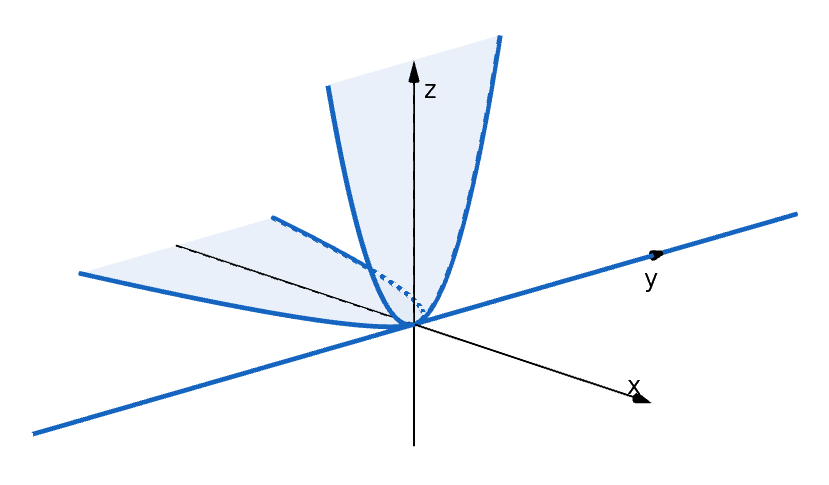
\includegraphics[width=10cm]{prim-descomp-ejemplo.png}
\end{center}

\begin{ejemplo}
  Hemos visto en \ref{ejemplo:potencia-de-primo-no-primaria-2} que el ideal
  $$\mathfrak{p} \dfn (f,g,h) \subset k [x,y,z], \quad f \dfn y^2 - xz, \quad g \dfn yz - x^3, \quad h \dfn z^2 - x^2y$$
  es primo, pero $\mathfrak{p}^2$ no es primario. Hagamos estos cálculos en
  \Mac{}.

  \begin{framed}\footnotesize
\begin{verbatim}
i1 : R = QQ[x,y,z];

i2 : (f,g,h) = (y^2 - x*z, y*z - x^3, z^2 - x^2*y);

i3 : P = ideal (f,g,h);

o3 : Ideal of R

i4 : isPrime P

o4 = true

i5 : isPrimary P^2

o5 = false

i6 : factor (g^2 - f*h)

          5      3     2       3
o6 = (x)(x  + x*y  - 3x y*z + z )

o6 : Expression of class Product

i7 : x % P == 0

o7 = false

i8 : pol = value o6#1

      5      3     2       3
o8 = x  + x*y  - 3x y*z + z

o8 : R

i9 : pol % P^2 == 0

o9 = false
\end{verbatim}
  \end{framed}
\end{ejemplo}

% % % % % % % % % % % % % % % % % % % % % % % % % % % % % %

\section{Dimensión de Krull}
\label{sec:dimension-de-Krull}

El concepto correcto de la dimensión en geometría algebraica y álgebra
conmutativa es la dimensión de Krull\footnote{\personality{Wolfgang Krull}
  (1899--1971) --- algebrista alemán conocido por sus contribuciones en álgebra
  conmutativa.}. Para motivar la definición, observemos que para un espacio
vectorial $V$ sobre un cuerpo $k$ la dimensión viene dada por
$$\dim_k V = \sup \{ n \mid \text{existe una cadena de subespacios } 0 = V_0 \subsetneq V_1 \subsetneq \cdots \subsetneq V_n = V \}.$$
La dimensión de Krull se define de manera parecida.

\begin{definicion}
  \label{dfn:dimension-de-Krull-espacios}
  La \term{dimensión de Krull} de un espacio topológico $X$ viene dada por
  $$\dim X \dfn \sup \{ n \mid \text{existe una cadena de subespacios cerrados irreducibles } X_0 \subsetneq X_1 \subsetneq \cdots \subsetneq X_n \subseteq X \}.$$
  Además, se pone
  $$\dim \emptyset \dfn -1.$$
\end{definicion}

\begin{ejercicio}
  Demuestre que si $X\ne \emptyset$ es un espacio noetheriano y $Z_1,\ldots,Z_s$
  son sus componentes irreducibles, entonces
  $$\dim X = \max \{ \dim Z_1, \ldots, \dim Z_s \}.$$
\end{ejercicio}

\begin{ejercicio}
  Demuestre que para un subespacio $Y\subseteq X$ se tiene
  $$\dim Y \le \dim X.$$
\end{ejercicio}

\begin{ejemplo}
  \label{ejemplo:conj-alg-de-dimension-0}
  Para un conjunto algebraico $X \subseteq \AA^n (k)$ se tiene $\dim X = 0$ si y
  solo si $X$ es finito y no vacío. En efecto, si $X$ es un conjunto finito,
  entonces la topología de Zariski sobre $X$ es discreta y los subconjuntos
  irreducibles de $X$ son unipuntuales. Entonces, todas las cadenas tienen
  longitud $0$. Viceversa, asumamos que $\dim X = 0$. El espacio $X$ es
  noetheriano y por ende tiene un número finito de componentes irreducibles,
  pero estas son unipuntuales, puesto que $\dim X = 0$.
\end{ejemplo}

Notamos que si $X$ es Hausdorff, entonces los subespacios irreducibles de $X$
son unipuntuales y la dimensión de $X$ será nula. Vamos a ocupar la definición
\ref{dfn:dimension-de-Krull-espacios} para la topología de Zariski que casi
nunca es Hausdorff.

Si $k$ es un cuerpo algebraicamente cerrado y $X \subseteq \AA^n (k)$ es un
conjunto algebraico, entonces una cadena de subespacios cerrados irreducibles
$$X_0 \subsetneq X_1 \subsetneq \cdots \subsetneq X_n \subseteq X$$
corresponde a una cadena de ideales primos
$$\mathfrak{p}_0 \subsetneq \mathfrak{p}_1 \subsetneq \cdots \subsetneq \mathfrak{p}_n \subset \Gamma (X).$$
Esto motiva la siguiente definición general.

\begin{definicion}
  \label{dfn:dimension-de-Krull-anillos}
  La \term{dimensión de Krull} de un anillo conmutativo $A$ viene dada por
  $$\dim A \dfn \sup \{ n \mid \text{existe una cadena de ideales primos } \mathfrak{p}_0 \subsetneq \mathfrak{p}_1 \subsetneq \cdots \subsetneq \mathfrak{p}_n \subset A \}.$$
  Además, por la definición,
  $$\dim 0 \dfn -1.$$
\end{definicion}

En particular, si $k$ es un cuerpo algebraicamente cerrado, entonces para un
conjunto algebraico $X \subseteq \AA^n (k)$ se tiene
$$\dim X = \dim \Gamma (X).$$

\begin{comentario}
  En efecto, la definición \ref{dfn:dimension-de-Krull-anillos} se obtiene
  aplicando \ref{dfn:dimension-de-Krull-espacios} al espacio $\Spec A$ con
  la topología de Zariski definida en \ref{digresion:topologia-sobre-Spec}.
\end{comentario}

\begin{ejemplo}
  Para todo cuerpo $k$ se tiene $\dim k = 0$, dado que $\Spec k = \{ (0) \}$.
  En general, recordemos que un anillo $A$ es \term{artiniano} si y solo si $A$
  es noetheriano y todo ideal primo en $A$ es maximal. En este caso las cadenas
  de ideales primos tienen longitud $0$ y por ende $\dim A = 0$.
\end{ejemplo}

\begin{ejemplo}
  Si $A$ es un dominio de ideales principales, como por ejemplo $\ZZ$ o $k [x]$,
  entonces $\dim A = 1$. Esto se sigue del hecho de que los ideales primos en
  $A$ son $(0)$ y los ideales maximales $(p)$, donde $p \in A$ es un elemento
  primo. Entonces, toda cadena de ideales primos de longitud maximal tiene forma
  $$(0) \subsetneq (p) \subset A.$$
  Esto también demuestra que
  $$\dim \AA^1 (k) = 1, \quad\text{si }k\text{ es infinito}.$$
  De hecho, tenemos una cadena de subconjuntos irreducibles
  $$\{ 0 \} = \mathbf{V} (x) \subsetneq \mathbf{V} (0) = \AA^1 (k),$$
  y viceversa, toda cadena de subconjuntos cerrados irreducibles en $\AA^1 (k)$
  corresponde a una cadena de ideales primos en $k [x]$ que tiene longitud
  $\le 1$.
\end{ejemplo}

\begin{ejemplo}
  En el anillo de polinomios en número finito de variables existe una cadena
  infinita de ideales primos
  $$(0) \subsetneq (x_1) \subsetneq (x_1,x_2) \subsetneq (x_1,x_2,x_3) \subsetneq \cdots \subset k [x_1,x_2,x_3,\ldots],$$
  así que
  $$\dim k [x_1,x_2,x_3,\ldots] = \infty.$$
  Este anillo no es noetheriano. En general, existen anillos no noetherianos de
  dimensión finita y anillos noetherianos de dimensión infinita\footnote{El
    hecho de que todas las cadenas de ideales se estabilizan no necesariamente
    significa que hay una cota para la longitud de cadenas.}. Ejemplos
  específicos de tales anillos fueron descubiertos por el algebrista japonés
  \personality{Masayoshi Nagata}. Sin embargo, aquí nos va a interesar el caso
  de $k$-álgebras finitamente generadas, donde la dimensión se comporta bien.
\end{ejemplo}

\begin{ejercicio}
  Sean $A$ un anillo e $I \subseteq A$ un ideal. Demuestre que
  $\dim (A/I) \le \dim A$.
\end{ejercicio}

\begin{ejercicio}
  Demuestre que para el producto de dos anillos se tiene
  $$\dim (A\times B) = \max \{ \dim A, \dim B \}.$$
\end{ejercicio}

\begin{ejercicio}
  Sea $k$ un cuerpo. Demuestre que el anillo de las series formales
  $k [\![x]\!]$ y el anillo de polinomios de Laurent $k [x,x^{-1}]$ tienen
  dimensión $1$.
\end{ejercicio}

\begin{ejercicio}
  Demuestre que el anillo $\ZZ [x]$ tiene dimensión $2$.
\end{ejercicio}

\subsection{Dimensión y el grado de trascendencia}

Intuitivamente, la dimensión del espacio afín $\AA^n (k)$ debe ser igual a
$n$. En el anillo $\Gamma (\AA^n (k)) = k [x_1,\ldots,x_n]$ tenemos la cadena de
ideales primos
$$0 \subsetneq (x_1) \subsetneq (x_1,x_2) \subsetneq \cdots \subsetneq (x_1,x_2,\ldots,x_n) \subset k [x_1,\ldots,x_n]$$
que en el caso de $k$ infinito corresponde a la cadena de subespacios
irreducibles
\begin{equation}
  \label{eqn:cadena-en-Ank}
  \mathbf{V} (x_1,x_2,\ldots,x_n) \subsetneq \cdots \subsetneq \mathbf{V} (x_1,x_2) \subsetneq \mathbf{V} (x_1) \subsetneq \AA^n (k).
\end{equation}
Notamos que esto demuestra solamente las desigualdades
$$\dim \AA^n (k) \ge n, \quad\text{si }k\text{ es infinito}$$
y
$$\dim k [x_1,\ldots,x_n] \ge n.$$
---no está claro por qué no existen cadenas más largas. Para resolver este
problema, vamos a relacionar la dimensión de Krull con otro invariante: el grado
de trascendencia.

\begin{definicion}
  Sea $A$ un álgebra sobre un cuerpo $k$. Digamos que $a_1,\ldots,a_s \in A$ son
  \term{algebraicamente independientes} sobre $k$ si para todo polinomio no nulo
  $f \in k[x_1,\ldots,x_s]$ se tiene
  $$f (a_1,\ldots,a_s) \ne 0.$$
  El \term{grado de trascendencia} de $A$ se define mediante
  $$\trdeg_k A \dfn \sup \{ \#S \mid S \subset A\text{ un subconjunto finito, algebraicamente independiente sobre }k \}.$$
  Además, se pone
  $$\trdeg_k 0 \dfn -1.$$
\end{definicion}

\begin{ejemplo}
  Dejo al lector digerir la definición de arriba y entender que para el anillo
  de polinomios $k [x_1,\ldots,x_n]$ un subconjunto maximal algebraicamente
  independiente viene dado por $S = \{ x_1, \ldots, x_n \}$, y por ende
  $$\trdeg_k (k [x_1,\ldots,x_n]) = n.$$
  De la misma manera, para el cuerpo de funciones racionales
  $$k (x_1,\ldots,x_n) \dfn \Frac (k [x_1,\ldots,x_n])$$
  se tiene
  \[ \trdeg_k (k (x_1,\ldots,x_n)) = n. \qedhere \]
\end{ejemplo}

\begin{teorema}
  \label{thm:dim-y-trdeg}
  Sean $A$ una $k$-álgebra y $S \subset A$ un conjunto de generadores de $A$
  como $k$-álgebra. Entonces,
  $$\dim A \le \sup \{ \#T \mid T \subseteq S\text{ subconjunto finito, algebraicamente independiente} \}  \le \trdeg_k A.$$
  Además, si $A$ es finitamente generada, entonces se cumplen igualdades
  $$\dim A = \sup \{ \#T \mid T \subseteq S\text{ subconjunto finito, algebraicamente independiente} \} = \trdeg_k A.$$
\end{teorema}

\begin{comentario}
  En general, cuando $A$ no es finitamente generada, la desigualdad es estricta:
  por ejemplo, como todo cuerpo, ${k (x_1,\ldots,x_n)}$ tiene dimensión de Krull
  $0$, aunque $\trdeg_k (k (x_1,\ldots,x_n)) = n$.
\end{comentario}

Antes de probar el teorema, notamos que como un caso particular se obtiene el
siguiente resultado.

\begin{corolario}
  Para cualquier cuerpo $k$ se tiene $\dim k [x_1,\ldots,x_n] = n$.
\end{corolario}

\begin{corolario}
  Para el espacio afín se tiene
  $$\dim \AA^n (k) = \begin{cases}
    n, & \text{si }k\text{ es infinito},\\
    0, & \text{si }k\text{ es finito}.
  \end{cases}$$

  \begin{proof}
    Si $k = \FF_q$ es un cuerpo finito, entonces $\dim \AA^n (\FF_q) = 0$
    gracias a la observación en \ref{ejemplo:conj-alg-de-dimension-0}. Si $k$ es
    infinito, entonces tenemos una cadena de subconjuntos irreducibles
    \eqnref{eqn:cadena-en-Ank} de longitud $n$, así que
    $$\dim \AA^n (k) \ge n.$$
    Viceversa, una cadena de subconjuntos irreducibles
    $$X_0 \subsetneq X_1 \subsetneq \cdots \subsetneq X_m = \AA^n (k)$$
    nos da una cadena de ideales primos
    $$0 = \mathbf{I} (X_m) \subsetneq \cdots \subsetneq \mathbf{I} (X_1) \subsetneq \mathbf{I} (X_0) \subset k [x_1,\ldots,x_n],$$
    pero su longitud es necesariamente $\le \dim k [x_1,\ldots,x_n] = n$, lo que
    nos da la otra desigualdad
    \[ \dim \AA^n (k) \le n. \qedhere \]
  \end{proof}
\end{corolario}

\begin{comentario}
  En general, es cierto que para cualquier anillo noetheriano $A \ne 0$ se tiene
  $$\dim A[x] = \dim A + 1,$$
  pero no lo vamos a probar en nuestro breve curso. Note que esto implica por
  inducción que
  $$\dim k[x_1,\ldots,x_n] = n.$$
\end{comentario}

\subsection*{Demostración del teorema \ref{thm:dim-y-trdeg}}

Para un conjunto de generadores $S \subset A$ pongamos
$$n \dfn \sup \{ \#T \mid T \subseteq S\text{ subconjunto finito, algebraicamente independiente} \}.$$
Tenemos que probar que
$$\dim A \le n.$$

\begin{enumerate}
\item[1)] Notamos que es suficiente probar la desigualdad para el caso cuando
  $A$ es un dominio.

  En efecto, si una cadena de ideales primos de longitud maximal viene dada por
  $$\mathfrak{p} \subsetneq \mathfrak{p}_1 \subsetneq \cdots \subsetneq \mathfrak{p}_n \subset A,$$
  a esta cadena corresponde una cadena en $A/\mathfrak{p}$ de la misma longitud:
  $$(0) \subsetneq \mathfrak{p}_1/\mathfrak{p} \subsetneq \cdots \subsetneq \mathfrak{p}_n/\mathfrak{p} \subset A/\mathfrak{p}.$$
  Además, al remplazar $A$ por $A/\mathfrak{p}$ y el conjunto $S \subset A$ por
  $$S/\mathfrak{p} \dfn \{ a + \mathfrak{p} \mid a\in S \} \subset A/\mathfrak{p},$$
  el número $n$ no puede volverse más grande.

  Entonces, a partir de ahora podemos asumir que $A$ es un dominio.

\item[2)] Si $n = 0$, entonces todos los elementos de $S$ son algebraicos sobre
  $k$, lo que significa que el cuerpo de fracciones $\Frac A$ está generado como
  $k$-álgebra por elementos algebraicos sobre $k$, así que $\Frac A / k$ es una
  extensión algebraica. En particular, todos los elementos de $A$ son
  algebraicos sobre $k$. Ahora, dado que
  $$k \subset A \subset \Frac A,$$
  donde $\Frac A / k$ es una extensión algebraica, podemos concluir que $A$ es
  también un cuerpo (véase el lema
  \ref{lema:subalgebra-en-extension-algebraica}), y luego $\dim A = 0$.

\item[3)] Ahora asumamos que $n > 0$. Toda una cadena de ideales primos de
  longitud $m > 0$
  $$\mathfrak{p}_0 \subsetneq \mathfrak{p}_1 \subsetneq \cdots \subsetneq \mathfrak{p}_m \subset A$$
  nos da la cadena correspondiente de longitud $m-1$ en $A/\mathfrak{p}_1$:
  $$0 \subsetneq \mathfrak{p}_2/\mathfrak{p}_1 \subsetneq \cdots \subsetneq \mathfrak{p}_m/\mathfrak{p}_1 \subset A/\mathfrak{p}_1.$$
  Para el paso inductivo sería suficiente probar que todos los subconjuntos
  algebraicamente independientes $T \subseteq S/\mathfrak{p}_1$ tienen $< n$
  elementos: en este caso
  $$m-1 \le \dim (A/\mathfrak{p}_1) < n$$
  por la hipótesis inductiva, y luego $m \le n$. Asumamos que existen $n$
  elementos $a_1,\ldots,a_n \in S$ tales que
  $$a_1 + \mathfrak{p}_1, \ldots, a_n + \mathfrak{p}_1 \in A/\mathfrak{p}_1$$
  son $n$ diferentes elementos algebraicamente independientes sobre $k$. Luego,
  $a_1,\ldots,a_n \in A$ son también algebraicamente independientes. Ahora por
  la elección de $n$, todo elemento de $S$ es algebraico sobre el cuerpo
  $$k (a_1,\ldots,a_n) = \Frac k [x_1,\ldots,x_n].$$
  Los elementos de $S$ son generadores de $A$, así que $\Frac A$ es una
  extensión algebraica de $L$. En particular, para un elemento no nulo
  $a \in \mathfrak{p}_1$ existen $f_0,f_1,\ldots,f_s \in k (a_1,\ldots,a_n)$
  tales que
  $$f_s\,a^s + f_{s-1}\,a^{s-1} + \cdots + f_1\,a + f_0 = 0.$$
  Sin pérdida de generalidad, $f_0 \ne 0$. Además, multiplicando los $f_i$ por
  su común denominador, podemos asumir que
  $f_0,f_1,\ldots,f_s \in k [a_1,\ldots,a_n]$. Luego,
  $$f_0 = -(f_s\,a^{s-1} + f_{s-1}\,a^{s-2} + \cdots + f_1)\,a \in \mathfrak{p}_1.$$
  Ahora $f_0$ corresponde a un polinomio $F_0 \in k [x_1,\ldots,x_n]$ evaluado
  en $a_1,\ldots,a_n$, pero la expresión de arriba significa que
  $a_1 + \mathfrak{p}_1, \ldots, a_n + \mathfrak{p}_1$ son algebraicamente
  dependientes. Contradicción.
\end{enumerate}

Ahora nos gustaría probar que cuando $A$ es un álgebra finitamente generada,
entonces se tiene la otra desigualdad
$$\trdeg_k A \le \dim A.$$
Vamos a probar que si existen $n$ elementos $a_1,\ldots,a_n \in A$
algebraicamente independientes sobre $k$, entonces en $A$ existe una cadena
de ideales primos de longitud $n$.

\begin{enumerate}
\item[1)] Como antes, sin pérdida de generalidad, se puede asumir que $A$ es un
  dominio. En efecto, en este caso $A$ es noetheriano y tiene un número finito
  de ideales primos minimales $\mathfrak{p}_1,\ldots,\mathfrak{p}_s$.
  Su intersección coincide con el nilradical:
  $$\mathfrak{p}_1 \cap \cdots \cap \mathfrak{p}_s = N (A).$$
  Si $a_1,\ldots,a_n \in A$ son algebraicamente independientes sobre $k$,
  entonces existe $i = 1,\ldots,s$ tal que los elementos
  ${a_1 + \mathfrak{p}_i}, \ldots, {a_n + \mathfrak{p}_i} \in A/\mathfrak{p}_i$
  son algebraicamente independientes. En efecto, si esto no es el caso, entonces
  para todo $i$ habrá un polinomio no nulo $f_i \in k [x_1,\ldots,x_n]$ tal que
  $f_i (a_1,\ldots,a_n) \in \mathfrak{p}_i$. Consideremos entonces el polinomio
  $$f \dfn f_1\cdots f_s \ne 0.$$
  Tenemos
  $$f (a_1,\ldots,a_n) \in \mathfrak{p}_1 \cap \cdots \cap \mathfrak{p}_s = N (A),$$
  pero esto implica que existe $r = 1,2,3,\ldots$ tal que
  $f^r (a_1,\ldots,a_n) = 0$, lo que contradice la independencia algebraica
  de $a_1,\ldots,a_n$.

  Ahora si a partir de los elementos algebraicamente independientes
  $a_1 + \mathfrak{p}_i, \ldots, a_n + \mathfrak{p}_i \in A/\mathfrak{p}_i$
  se puede obtener una cadena de ideales primos de longitud $n$
  en $A/\mathfrak{p}_i$, esta cadena nos dará una cadena de ideales primos
  de longitud $n$ en $A$.

  A partir de ahora podemos asumir que $A$ es un dominio.

\item[2)] La base de inducción es obvia: en $A$ hay un ideal primo, por ejemplo
  $(0)$, que nos da una cadena de longitud $0$.

\item[3)] Consideremos el subcuerpo
  $$L \dfn K (a_1) \subseteq \Frac A$$
  y la subálgebra
  $$A' \dfn L\cdot A \subseteq \Frac A.$$
  Notamos que $A'$ es una $L$-álgebra y $a_2,\ldots,a_n \in A'$ son
  algebraicamente independientes sobre $L$. Por la hipótesis inductiva,
  $\dim A \ge n-1$ y existe una cadena de ideales primos
  $$\mathfrak{p}_0' \subsetneq \mathfrak{p}_1'  \subsetneq \cdots \subsetneq \mathfrak{p}_{n-1}' \subset A'.$$
  Pongamos entonces
  $$\mathfrak{p}_i \dfn \mathfrak{p}_i' \cap A.$$
  Dado que $L\cdot \mathfrak{p}_i = \mathfrak{p}_i'$, tenemos una cadena de
  ideales primos
  $$\mathfrak{p}_0 \subsetneq \mathfrak{p}_1  \subsetneq \cdots \subsetneq \mathfrak{p}_{n-1} \subset A.$$
  El ideal $\mathfrak{p}_{n-1} \subset A$ no es maximal. En efecto, si
  $\mathfrak{p}_{n-1}$ fuera maximal, el cuerpo $A/\mathfrak{p}_{n-1}$ sería una
  extensión finita de $k$ y el elemento
  $a_1 + \mathfrak{p}_{n-1} \in A/\mathfrak{p}_{n-1}$ sería algebraico sobre
  $k$. Luego,
  $$c_n\,a_1^n + c_{n-1}\,a_1^{n-1} + \cdots + c_1\,a_1 + c_0 \in \mathfrak{p}_{n-1}$$
  para algunos $c_n,c_{n-1},\ldots,c_0 \in k$, donde $c_0 \ne 0$. Sin embargo,
  esto demostraría que
  $$c_0 = -(c_n\,a_1^n + c_{n-1}\,a_1^{n-1} + \cdots + c_1\,a_1) \in \mathfrak{p}_{n-1}',$$
  y luego $\mathfrak{p}_{n-1}' = A'$, que no es el caso.

  Entonces, el ideal primo $\mathfrak{p}_{n-1}$ no es maximal en $A$ y existe un
  ideal maximal $\mathfrak{p}_{n-1} \subsetneq \mathfrak{p}_n \subset A$. Esto
  nos da una cadena de longitud $n$
  $$\mathfrak{p}_0 \subsetneq \mathfrak{p}_1  \subsetneq \cdots \subsetneq \mathfrak{p}_{n-1} \subsetneq \mathfrak{p}_n \subset A$$
  y concluye la prueba. \qed
\end{enumerate}

Este argumento viene de \cite{Kemper-GTM-256}.

\subsection{Cálculo de dimensión}

\begin{corolario}[Dimensión de álgebras finitamente generadas y eliminación]
  \label{cor:dimension-y-eliminacion}
  La dimensión del álgebra finitamente generada $A = k[x_1,\ldots,x_n]/I$ es el
  máximo número $\delta$ tal que existen variables
  $\{ x_{i_1}, \ldots, x_{i_\delta} \} \subseteq \{ x_1, \ldots, x_n \}$ que
  cumplen
  \begin{equation}
    \label{eqn:dimension-de-algebra-afin-eliminacion}
    I \cap k [x_{i_1},\ldots,x_{i_\delta}] = 0.
  \end{equation}

  \begin{proof}
    La condición $I \cap k [x_{i_1},\ldots,x_{i_\delta}] = 0$ significa
    precisamente que $\overline{x_{i_1}}, \ldots, \overline{x_{i_\delta}} \in A$
    son algebraicamente independientes sobre $k$.
  \end{proof}
\end{corolario}

\begin{corolario}
  \label{cor:dimension-de-conj-alg-y-eliminacion}
  Sean $k$ un cuerpo algebraicamente cerrado y $X \subseteq \AA^n (k)$ un
  conjunto algebraico. Entonces, $\dim X$ es el máximo número $\delta$ tal que
  existen $\delta$ variables
  $\{ x_{i_1}, \ldots, x_{i_\delta} \} \subseteq \{ x_1, \ldots, x_n \}$ que
  cumplen
  $$\mathbf{I} (X) \cap k [x_{i_1},\ldots,x_{i_\delta}] = 0.$$

  \begin{proof}
    Tenemos $\dim X = \dim k[x_1,\ldots,x_n]/\mathbf{I} (X)$.
  \end{proof}
\end{corolario}

Notamos que la condición \eqnref{eqn:dimension-de-algebra-afin-eliminacion}
puede ser verificada usando las bases de Gröbner, como hemos visto
en \S\ref{sec:eliminacion}. Esto nos da un algoritmo para calcular la dimensión
de una $k$-álgebra finitamente generada. Veamos un par de ejemplos.

\begin{ejemplo}
  \label{ejemplo:dim-xz-yz}
  Calculemos la dimensión del álgebra afín $k [x,y,z]/I$ donde
  $I = (xz, yz)$. Notamos que a este ideal monomial corresponde el conjunto
  algebraico
  $$\mathbf{V} (I) = \mathbf{V} (x,y) \cup \mathbf{V} (z)$$
  que es la unión del eje $z$ y el plano $xy$.

  \begin{center}
    \begin{tikzpicture}
      \fill[color=blue, fill opacity=0.3] (3/2,1/2) -- (1/2,-1/2) -- (-3/2,-1/2) -- (-1/2,1/2);
      \draw[->] (0,-3/2) -- (0,3/2) node[above] {$z$};
      \draw[->] (-3/2,0) -- (3/2,0) node[right] {$x$};
      \draw[->] (3/4,3/4) -- (-3/4,-3/4) node[below left] {$y$};
    \end{tikzpicture}
  \end{center}

  Tenemos $I \ne 0$, y luego
  $$I \cap k [y,z] = (yz), \quad I \cap k [x,z] = (xz), \quad I \cap k [x,y] = 0$$
  (es fácil verificar estas intersecciones, dado que el ideal en cuestión es
  monomial). La última intersección nos permite concluir que
  $\dim k [x,y,z]/I = 2$.
\end{ejemplo}

\begin{ejemplo}
  \label{ejemplo:dim-cubica-torcida}
  Calculemos la dimensión del álgebra afín $k [x,y,z]/I$, donde
  $I = (x^2-y, x^3-z)$. Tenemos
  $$I \cap k [x,y] = (x^2-y), \quad k [x,z] = (x^3-z), \quad I \cap k [y,z] = (y^3-z^2).$$
  Estos cálculos pueden ser verificados en \Mac{}:

  \begin{framed}\footnotesize
\begin{verbatim}
i1 : R = QQ[x,y,z];

i2 : I = ideal (x^2-y, x^3-z);
o2 : Ideal of R

i3 : eliminate (x,I)

            3    2
o3 = ideal(y  - z )
o3 : Ideal of R

i4 : eliminate (y,I)

            3
o4 = ideal(x  - z)
o4 : Ideal of R

i5 : eliminate (z,I)

            2
o5 = ideal(x  - y)
o5 : Ideal of R
\end{verbatim}
  \end{framed}

  Entonces, la dimensión de $k [x,y,z]/I$ tiene que ser menor que $2$. Luego,
  calculamos que
  $$I \cap k [x] = I \cap k [y] = I \cap k [z] = 0,$$
  de donde $\dim k [x,y,z]/I = 1$.

  \begin{framed}\footnotesize
\begin{verbatim}
i6 : eliminate ({x,y},I)
o6 = ideal ()
o6 : Ideal of R

i7 : eliminate ({x,z},I)
o7 = ideal ()
o7 : Ideal of R

i8 : eliminate ({y,z},I)
o8 = ideal ()
o8 : Ideal of R
\end{verbatim}
  \end{framed}

  De hecho, tenemos
  $$k [x,y,z]/(x^2-y, \, x^3-z) \isom k[x,x^2,x^3] \isom k [x],$$
  y ya sabemos que la dimensión de $k [x]$ es igual a $1$. Geométricamente, el
  conjunto algebraico $\mathbf{V} (I)$ es la cúbica torcida que es isomorfa a la
  recta afín $\AA^1 (k)$ (véase \ref{ejemplo:cubica-torcida}).
\end{ejemplo}

\begin{ejercicio}
  Encuentre la dimensión de las $k$-álgebras
  $$k[x,y,z]/(xz, xy - 1), \quad k[x,y,z,w]/(zw - y^2 , xy - z^3)$$
  usando el método de arriba.
\end{ejercicio}

\begin{ejercicio}
  Demuestre que para toda $k$-álgebra finitamente generada se cumple
  $$\dim A = 0 \iff \dim_k (A) < \infty,$$
  donde $\dim$ denota la dimensión de Krull y $\dim_k$ denota la dimensión
  de espacio vectorial sobre $k$..
\end{ejercicio}

Desafortunadamente, para encontrar el número máximo de variables
$x_{i_1}, \ldots, x_{i_s}$ que satisfacen la condición
\eqnref{eqn:dimension-de-algebra-afin-eliminacion}, en general habrá que
calcular un montón de bases de Gröbner (y respecto a órdenes monomiales
ineficaces), así que este método no es muy práctico. Más adelante vamos
a estudiar las series de Hilbert que es otra herramienta más eficaz para
calcular la dimensión a partir de una sola base de Gröbner de $I$ respecto
al orden \emph{grlex} o \emph{grevlex}.

Terminemos por una aplicación teórica de
\ref{cor:dimension-de-conj-alg-y-eliminacion}.

\begin{teorema}
  Sean $k$ un cuerpo algebraicamente cerrado y $X\subseteq \AA^m (k)$ e
  $Y\subseteq \AA^n (k)$ dos conjuntos algebraicos no vacíos. Entonces, su
  producto $X\times Y \subseteq \AA^{m+n} (k)$ satisface
  $$\dim (X\times Y) = \dim X + \dim Y.$$

  \begin{proof}
    Tenemos $\mathbf{I} (X) \subseteq k [x_1,\ldots,x_m]$ y
    $\mathbf{I} (Y) \subseteq k [y_1,\ldots,y_n]$. Sea
    $$d = \dim X = \dim k [x_1,\ldots,x_m]/\mathbf{I} (X), \quad e = \dim Y = \dim k [y_1,\ldots,y_n]/\mathbf{I} (Y).$$
    Según el corolario \ref{cor:dimension-de-conj-alg-y-eliminacion}, $d$ y $e$
    corresponden al máximo número de variables $x_{i_1},\ldots,x_{i_d}$ e
    $y_{j_1}, \ldots, y_{j_e}$ respectivamente tales que
    $$\mathbf{I} (X) \cap k [x_{i_1}, \ldots, x_{i_d}] = 0, \quad \mathbf{I} (Y) \cap k [y_{j_1}, \ldots, y_{j_e}] = 0.$$
    Ahora un polinomio
    $$f \in \mathbf{I} (X\times Y) \cap k [x_{i_1}, \ldots, x_{i_d}, y_{j_1}, \ldots, y_{j_e}]$$
    puede ser escrito como
    $$f = \sum_\alpha f_\alpha\,y_{j_1}^{\alpha_1}, \ldots, y_{j_e}^{\alpha_e},$$
    donde $f_\alpha \in k [x_{i_1}, \ldots, x_{i_d}]$. Luego, para todo punto
    $(a_1,\ldots,a_m) \in X$ se tiene
    $$\sum_\alpha f_\alpha (a_1,\ldots,a_m)\,y_{j_1}^{\alpha_1} \in \mathbf{I} (Y) \cap k [y_{j_1},\ldots,y_{j_e}],$$
    así que
    $$\sum_\alpha f_\alpha (a_1,\ldots,a_m)\,y_{j_1}^{\alpha_1} = 0.$$
    Esto implica que $f_\alpha (a_1,\ldots,a_m) = 0$ todo
    $(a_1,\ldots,a_m)$. Luego,
    $$f_\alpha \in \mathbf{I} (X) \cap k [x_{i_1},\ldots,x_{i_d}],$$
    así que $f_\alpha = 0$ para todo $\alpha$ y $f = 0$. Esto demuestra que
    $$\mathbf{I} (X\times Y) \cap k [x_{i_1}, \ldots, x_{i_d}, y_{j_1}, \ldots, y_{j_e}] = 0,$$
    y por ende
    $$\dim (X\times Y) \ge d+e.$$

    La otra desigualdad $\dim (X\times Y) \le d+e$ es más fácil. Si tenemos un
    subconjunto $T \subseteq \{ x_1,\ldots,x_m, y_1,\ldots,y_n \}$ tal que
    $\#T > d+e$, entonces
    $$\#(T \cap \{ x_1,\ldots,x_m \}) > d \quad\text{o}\quad \#(T \cap \{ y_1,\ldots,y_n \}) > d.$$
    Asumamos por ejemplo el primer caso. Existen entonces $s > d$ variables
    $x_{i_1},\ldots,x_{i_s} \in T$ tales que
    $$\mathbf{I} (X) \cap k [x_{i_1}, \ldots, x_{i_s}] \ne 0.$$
    Esto nos da un polinomio no nulo $f \in k [x_{i_1},\ldots,x_{i_s}]$ que se
    anula en todos los puntos de $X$. Luego, $f$ se anula en todos los puntos de
    $X\times Y$ e
    \[ \mathbf{I} (X\times Y) \cap k [x_{i_1}, \ldots, x_{i_s}] \ne 0. \qedhere \]
  \end{proof}
\end{teorema}

\begin{comentario}
  El análogo algebraico del último resultado es la identidad
  $$\dim (A\otimes_k B) = \dim A + \dim B$$
  para $k$-álgebras finitamente generadas (véase el ejercicio
  \ref{ejerc:Gamma-X-times-Y}). Notamos que en particular,
  $$\dim k [x_1,\ldots,x_n] = \dim (k [x_1]\otimes_k \cdots \otimes_k k [x_n]) = \dim k[x_1] + \cdots + \dim k [x_n] = n.$$
  En general, afuera del mundo de $k$-álgebras finitamente generadas,
  los productos tensoriales no se comportan bien respecto a la dimensión.
  Por ejemplo, si $p$ y $q$ son diferentes primos, entonces
  $$\Spec \FF_p = \{ (0) \}, \quad \Spec \FF_q = \{ (0) \}, \quad \Spec (\FF_p\otimes_\ZZ\FF_q) = \emptyset.$$
\end{comentario}

\subsection{Dimensión de Krull en \Mac}

Si $A$ es un cociente del anillo de polinomios $k [x_1,\ldots,x_n]$
(donde $k = \QQ$ o $\FF_q$), la dimensión de $A$ puede ser calculada en \Mac{}
mediante \texttt{dim($A$)}. Para un ideal $I \subseteq k [x_1,\ldots,x_n]$,
el comando \texttt{dim($I$)} calcula la dimensión del anillo cociente
$k [x_1,\ldots,x_n]/I$.

He aquí un pequeño ejemplo.

\begin{framed}\footnotesize
\begin{verbatim}
i1 : R = QQ[x,y,z];

i2 : dim R
o2 = 3

i3 : dim ideal (0_R)
o3 = 3

i4 : dim ideal (x)
o4 = 2

i5 : dim ideal (x,y)
o5 = 1

i6 : dim ideal (x,y,z)
o6 = 0

i7 : dim ideal (x*z,y*z)
o7 = 2

i8 : dim ideal (x^2-y,x^3-z)
o8 = 1
\end{verbatim}
\end{framed}

% % % % % % % % % % % % % % % % % % % % % % % % % % % % % %

\section{Digresión sobre las series formales}

El \term{anillo de las series formales} con coeficientes enteros en la variable
$t$ se denota por $\ZZ [\![t]\!]$. Sus elementos son las sumas formales
$$\sum_{d\ge 0} a_d\,t^d = a_0 + a_1\,t + a_2\,t^2 + a_3\,t^3 + \cdots,$$
donde $a_d \in \ZZ$. A diferencia de los polinomios, \emph{no se pide} que
$a_d = 0$ para $d$ suficientemente grande. Las sumas y productos se definen de
la manera habitual:
$$\sum_{d\ge 0} a_d\,t^d + \sum_{d\ge 0} b_d\,t^d \dfn \sum_{d\ge 0} (a_d+b_d)\,t^d$$
y
$$\left(\sum_{p\ge 0} a_p\,t^p\right) \cdot \left(\sum_{q\ge 0} b_q\,t^q\right) \dfn \sum_{d\ge 0} \left(\sum_{p+q=d} a_p b_q\right)\,t^d.$$

\begin{ejercicio}
  Demuestre que una serie formal $\sum_{d\ge 0} a_d\,t^d \in \ZZ [\![t]\!]$ es
  invertible si y solamente si $a_0 = \pm 1$.
\end{ejercicio}

\begin{definicion}
  Las \term{derivadas formales} vienen dadas por
  $$\left(\sum_{d\ge 0} a_d\,t^d\right)' \dfn \sum_{d \ge 1} d\,a_d\,t^{d-1}.$$
\end{definicion}

\begin{ejercicio}
  Demuestre que para cualesquiera $f,g \in \ZZ [\![t]\!]$ se cumple
  $$(f+g)' = f' + g'$$
  y la regla de Leibniz
  $$(fg)' = f'g + fg'.$$
  Demuestre que para $f = a_0 + a_1\,t + a_2\,t^2 + \cdots$ se tiene
  $$d!\,a_d = f^{(d)} (0),$$
  donde $f^{(d)} (0)$ denota el término constante de la $d$-ésima derivada
  formal de $f$.
\end{ejercicio}

\begin{lema}
  Para todo $n \in \ZZ$ se tiene
  $$((1-t)^n)' = -n\,(1-t)^{n-1}.$$

  \begin{proof}
    Si $n \ge 0$, podemos proceder por inducción usando la regla de Leibniz. La
    base de inducción sería $n = 0,1$, y luego para $n \ge 2$
    \begin{multline*}
      ((1-t)^n)' = ((1-t)\,(1-t)^{n-1})' = (1-t)'\,(1-t)^{n-1} + (1-t)\,((1-t)^{n-1})' \\
      = -(1-t)^{n-1} - (1-t)\,(n-1)\,(1-t)^{n-2} = -n\,(1-t)^{n-1}.
    \end{multline*}

    Para exponentes negativos, podemos calcular usando la regla de Leibniz que en
    general, para cualquier serie invertible $f$ se tiene
    $$0 = (f\,f^{-1})' = f'\,f^{-1} + f\,(f^{-1})',$$
    de donde
    $$(f^{-1})' = -f'\,f^{-2}.$$
    En particular, para $n \ge 0$
    \[ ((1-t)^{-n})' = -((1-t)^n)'\,(1-t)^{-2n} = n\,(1-t)^{-n-1}. \qedhere \]
  \end{proof}
\end{lema}

\begin{corolario}
  Consideremos la serie $f \dfn (1-t)^n$ para $n \in \ZZ$. Luego, para cualquier
  $d \in \NN$ se cumple
  $$f^{(d)} = (-1)^d\,n\,(n-1)\cdots (n-d+1)\,(1-t)^{n-d}.$$

  \begin{proof}
    Inducción usando el cálculo anterior.
  \end{proof}
\end{corolario}

\begin{definicion}
  Para $n \in \ZZ$ y $d \in \NN$, el coeficiente binomial ${n \choose d}$ viene
  dado por
  \begin{equation}
    \label{eqn:coeficiente-binomial}
    {n \choose 0} \dfn 1, \quad {n \choose d} \dfn \frac{n\,(n-1)\,(n-2)\cdots (n-d+1)}{d!}\text{ para }d > 0.
  \end{equation}
\end{definicion}

Cuando $0 \le n \le d$, la expresión \eqnref{eqn:coeficiente-binomial} viene de
la fórmula conocida
$${n \choose d} = \frac{n!}{d!\,(n-d)!} \in \ZZ.$$
Además, la definición de arriba nos da
$${n \choose d} = 0 \text{, si }n > d.$$

\begin{lema}
  Para $n \in \ZZ$ y $d \in \NN$ se cumple
  \begin{equation}
    \label{eqn:coef-binom-negativo}
    {-n \choose d} = (-1)^d\,{n + d - 1 \choose d}.
  \end{equation}

  \begin{proof}
    Cálculo directo:
    \[ {-n \choose d} = \frac{-n\,(-n-1)\,(-n-2)\cdots (-n-d+1)}{d!} = (-1)^d\,\frac{n\,(n+1)\,(n+2)\cdots (n+d-1)}{d!} = (-1)^d\,{n + d - 1 \choose d}. \qedhere \]
  \end{proof}
\end{lema}

\begin{proposicion}[Serie binomial]
  Para todo $n \in \ZZ$ se cumple
  $$(1-t)^n = \sum_{d\ge 0} (-1)^d\,{n\choose d}\,t^d.$$

  \begin{proof}
    Los coeficientes de la serie $f = (1-t)^n$ cumplen
    $$d!\,a_d = f^{(d)} (0) = (-1)^d\,n\,(n-1)\cdots (n-d+1),$$
    y luego
    \[ a_d = \frac{(-1)^d\,n\,(n-1)\cdots (n-d+1)}{d!} = (-1)^d\,{n\choose d}. \qedhere \]
  \end{proof}
\end{proposicion}

Notamos que para $n > 0$ esta es la fórmula del binomio de toda la vida,
mientras que para $n < 0$ esta es una serie infinita.

\begin{ejemplo}
  Si $n = -1$, tenemos gracias a la fórmula \eqnref{eqn:coef-binom-negativo}
  $${-1\choose d} = (-1)^d,$$
  así que
  $$\frac{1}{1-t} = 1 + t + t^2 + t^3 + \cdots$$
  Si $n = -2$, entonces
  $${-2\choose d} = (-1)^d\,{d+1\choose d} = (-1)^d\,(d+1),$$
  así que
  \[ \frac{1}{(1-t)^2} = 1 + 2 t + 3 t^2 + 4 t^3 + \cdots \qedhere \]
\end{ejemplo}

\begin{corolario}[Identidad de Vandermonde]
  Para cualesquiera $m,n\in \ZZ$ se tiene
  $$\sum_{p+q = d} {m\choose p}\,{n\choose q} = {m+n \choose d}.$$

  \begin{proof}
    Compare los coeficientes de las series $(1-t)^m\cdot (1-t)^n$ y
    $(1-t)^{m+n}$.
  \end{proof}
\end{corolario}

Para hacer cálculos con las series formales, recomiendo el programa
PARI/GP. Para indicar que una expresión en $t$ es una serie con precisión hasta
el $n$-ésimo término, hay que añadir ``\texttt{+ O($t$\^{}$n$)}''. He aquí
algunos ejemplos.

\begin{framed}\footnotesize
\begin{verbatim}
? 1/(1-t) + O (t^10)
% = 1 + t + t^2 + t^3 + t^4 + t^5 + t^6 + t^7 + t^8 + t^9 + O(t^10)
? 1/(1-t)^2 + O (t^10)
% = 1 + 2*t + 3*t^2 + 4*t^3 + 5*t^4 + 6*t^5 + 7*t^6 + 8*t^7 + 9*t^8 + 10*t^9 + O(t^10)
? (-t^2+t+1)/(1-t)^2 + O (t^10)
% = 1 + 3*t + 4*t^2 + 5*t^3 + 6*t^4 + 7*t^5 + 8*t^6 + 9*t^7 + 10*t^8 + 11*t^9 + O(t^10)
? (1+t)/(1-t) + O (t^10)
% = 1 + 2*t + 2*t^2 + 2*t^3 + 2*t^4 + 2*t^5 + 2*t^6 + 2*t^7 + 2*t^8 + 2*t^9 + O(t^10)
\end{verbatim}
\end{framed}

\begin{ejercicio}
  Para $d \in \NN$ consideremos los polinomios
  $${x \choose d} \dfn \frac{x\,(x-1)\cdots (x-d+1)}{d!} \in \QQ [x].$$

  \begin{enumerate}
  \item[a)] Demuestre que
    $${x \choose 0} = 1, ~ {x \choose 1}, ~ {x \choose 2}, ~ \ldots, ~ {x\choose d}$$
    forman una base del $\QQ$-espacio vectorial formado por los polinomios
    racionales de grado $\le d$.

  \item[b)] Demuestre que todo polinomio $f \in \QQ [x]$ tal que $f (n) \in \ZZ$
    para todo $n\in \ZZ$ puede ser escrito como
    $$f = a_0 \, {x \choose 0} + a_1 \, {x \choose 1} + \cdots + a_d\,{x \choose d},$$
    donde $a_0, a_1,\ldots,a_d \in \ZZ$.
  \end{enumerate}
\end{ejercicio}

\begin{comentario}
  En \Mac{} la función \texttt{binomial\,($\alpha$,$n$)} calcula el coeficiente
  binomial
  $${\alpha \choose n} \dfn \frac{\alpha\,(\alpha-1)\cdots (\alpha-n+1)}{n!}$$
  He aquí un ejemplo:
  \begin{framed}\footnotesize
\begin{verbatim}
i : for i in 0..10 list binomial (i,2)

o = {0, 0, 1, 3, 6, 10, 15, 21, 28, 36, 45}
o : List

i : binomial (-2,5)
o = -6

i : R = QQ[x];

i : binomial (x,2)

    1 2   1
o = -x  - -x
    2     2

o : R

i : binomial (x+2,2) - 2*binomial (x,2) + binomial (x-1,2)

o = x + 2
o : R
\end{verbatim}
  \end{framed}
\end{comentario}

% % % % % % % % % % % % % % % % % % % % % % % % % % % % % %

\section{Series de Hilbert}

\begin{definicion}
  Para un monomio
  $x^\alpha = x_1^{\alpha_1}\cdots x_n^{\alpha_n} \in k [x_1,\ldots,x_n]$,
  su \term{grado (total)} viene dado por
  $$\deg (x^\alpha) \dfn \alpha_1 + \cdots + \alpha_n.$$
  Para un polinomio no nulo
  $f = \sum_\alpha c_\alpha\,x^\alpha \in k [x_1,\ldots,x_n]$ el grado viene
  dado por
  $$\deg f \dfn \max \{ \deg x^\alpha \mid c_\alpha \ne 0 \}.$$
  Además, pongamos
  $$\deg 0 \dfn -1.$$
\end{definicion}

\begin{definicion}
  Para un ideal $I \subseteq k [x_1,\ldots,x_n]$ y el álgebra
  $A \dfn k [x_1,\ldots,x_n]/I$, para $d = 0,1,2,\ldots$ consideremos los
  $k$-espacios vectoriales
  \begin{align*}
    k [x_1,\ldots,x_n]_{\le d} & \dfn \{ f \in k [x_1,\ldots,x_n] \mid \deg f \le d \},\\
    I_{\le d} & \dfn I \cap k [x_1,\ldots,x_n]_{\le d}.
  \end{align*}
  Pongamos entonces
  $$A_{\le d} \dfn k [x_1,\ldots,x_n]_{\le d}/I_{\le d} \isom \{ \overline{f} \in A \mid f \in k [x_1,\ldots,x_n], ~ \deg f \le d \}.$$
  Además, sea
  $$A_d \dfn A_{\le d}/A_{\le d-1}.$$
  La \term{función de Hilbert de $I$} viene dada por
  $$h_I\colon d \mapsto \dim_k (A_d)$$
  y la \term{serie de Hilbert de $I$} es la serie formal
  $$H_I (t) \dfn \sum_{d\ge 0} h_I (d)\,t^d \in \ZZ [\![t]\!].$$
\end{definicion}

\begin{comentario}
  En algunas fuentes como \cite{Cox-Little-OShea-intro} y \cite{Kemper-GTM-256}
  por una muy buena razón se considera otra definición
  $$\widetilde{h} (d) \dfn \dim_k (A_{\le d}), \quad \widetilde{H}_I (t) \dfn \sum_{d\ge 0} \widetilde{h}_I (d)\,t^d.$$
  Notamos que
  $$h (d) = \widetilde{h} (d) - \widetilde{h} (d-1),$$
  y luego
  $$H_I (t) = \sum_{d\ge 0} h_I (d)\,t^d = \sum_{d\ge 0} \widetilde{h}_I (d)\,t^d - t\,\sum_{d\ge 0} \widetilde{h}_I (d)\,t^d = (1-t)\,\widetilde{H}_I (t).$$
  De hecho, el lector notará que para nuestros propósitos será más razonable
  hacer cálculos con $\widetilde{H}_I$, pero no hemos tomado $\widetilde{H}_I$
  como la definición principal de la serie de Hilbert para seguir la convención
  adoptada por \Mac{} que usa $H_I$\footnote{La serie $\widetilde{H}_I$ es un
    caso particular de la serie de Hilbert de un \term{álgebra filtrada}
    $$\{ 0 \} \subseteq F_0 \subseteq F_1 \subseteq F_2 \subseteq \cdots \subseteq A,$$
    mientras que $H_I$ es un caso particular de la serie de Hilbert de un
    \term{álgebra graduada}
    $$A = \bigoplus_{d\ge 0} A_d.$$
    A toda álgebra filtrada se asocia un álgebra graduada con
    $A_d \dfn F_d/F_{d-1}$.}.
\end{comentario}

\begin{ejercicio}
  Demuestre que si $I \subseteq J$, entonces $H_I (t) = H_J (t)$ implica que
  $I = J$.
\end{ejercicio}

\subsection{Primeros ejemplos}

\begin{ejemplo}
  Consideremos el ideal nulo $I = (0) \subset k [x_1,\ldots,x_n]$. En este caso
  $$A_d \isom k [x_1,\ldots,x_n]_d \isom k \langle x_1^{\alpha_1}\cdots x_n^{\alpha_n} \mid \alpha_1+\cdots+\alpha_n = d \rangle.$$
  Necesitamos entonces contar los monomios de grado total $d$. Por ejemplo, para
  dos variables $x,y$ se tiene
  \begin{align*}
    d = 0\colon & 1,\\
    d = 1\colon & x,\,y,\\
    d = 2\colon & x^2,\,xy,\,y^2,\\
    d = 3\colon & x^3,\,x^2y,\,xy^2,\,y^3,\\
                & \cdots
  \end{align*}
  El número de monomios de grado total $d$ es $d+1$. La serie de Hilbert será
  $$1 + 2\,t + 3\,t^3 + 4\,t^3 + \cdots = \frac{1}{(1-t)^2}.$$
  Para tres variables $x,y,z$ se tiene
  \begin{align*}
    d = 0\colon & 1,\\
    d = 1\colon & x,\,y,\,z,\\
    d = 2\colon & x^2,\,xy,\,xz,\,y^2,\,yz,\,z^2,\\
    d = 3\colon & x^3,\,x^2y,\,x^2z,\,xy^2,\,xyz,\,xz^2,\,y^3,\,y^2z,\,yz^2,\,z^3,\\
                & \cdots
  \end{align*}
  El número de monomios de grado total $d$ es ${d + 2\choose 2}$. En general, en
  $k [x_1,\ldots,x_n]$ el número de monomios de grado total $d$ es
  $${n+d-1 \choose d} = (-1)^d\,{-n \choose d}.$$
  Usando la serie binomial, calculamos que la serie de Hilbert viene dada por
  \[ H_{(0)} (t) = \sum_{d\ge 0} {n+d-1 \choose d} \, t^d = \sum_{d\ge 0} (-1)^d {-n \choose d} \, t^d = \sum_{d\ge 0} {-n \choose d} \, (-t)^d = \frac{1}{(1-t)^n}. \qedhere \]
\end{ejemplo}

\begin{ejercicio}
  Demuestre que el número de monomios $x_1^{\alpha_1}\cdots x_n^{\alpha_n}$ con
  $\alpha_1+\cdots+\alpha_n = d$ es igual a ${n+d-1 \choose d}$.
\end{ejercicio}

Notamos que si el ideal $I$ es monomial, entonces $I_{\le d}$ como espacio
vectorial sobre $k$ tiene una base que consiste en los monomios
$$x^\alpha = x_1^{\alpha_1}\cdots x_n^{\alpha_n} \in I, \quad \alpha_1+\cdots+\alpha_n \le d.$$
Luego,
$$A_d \isom k \left<x^\alpha \mid x^\alpha \notin I, ~ \alpha_1+\cdots+\alpha_n = d \right>.$$

\begin{ejemplo}
  \label{ejemplo:serie-de-Hilbert-xz-yz}
  Consideremos el ideal monomial $I = (xz,yz) \subset k [x,y,z]$.
  Para el álgebra $A \dfn k [x,y,z]/I$, la dimensión del espacio $A_d$
  corresponde al número de monomios de grado total $d$ que no son divisibles por
  $xz$ o $yz$, y son los siguientes:
  \begin{align*}
    d = 0\colon & 1,\\
    d = 1\colon & x,\,y,\,z,\\
    d = 2\colon & x^2,\,xz,\,y^2,\,z^2,\\
    d = 3\colon & x^3,\,x^2z,\,xz^2,\,y^3,\,z^3,\\
    d = 4\colon & x^4,\,x^3z,\,x^2z^2,\,xz^3,\,y^4,\,z^4,\\
                & \cdots
  \end{align*}
  En general, para $d > 0$ habrá $d+1$ monomios de la forma $x^a\,y^b$, donde
  $a+b = d$, más el monomio $z^d$. Esto significa que la función de Hilbert
  viene dada por
  $$h_I (d) = \begin{cases}
    1, & d = 0,\\
    d+2, & d > 0,
  \end{cases}$$
  y la serie de Hilbert correspondiente es
  \[ H_I (t) = 1 + 3t + 4t^2 + 5t^3 + 6t^4 + \cdots = \frac{1}{t\,(1-t)^2} - \frac{1}{t} - 1 = \frac{-t^2+t+1}{(1-t)^2}. \qedhere \]
\end{ejemplo}

\begin{ejercicio}
  \label{ejerc:series-de-Hilbert-ideales-monomiales}
  Calcule las series de Hilbert de los siguientes ideales monomiales en
  $k [x,y,z]$:
  $$(x^2, \, y^2, \, z^2), \quad (xy, \, xz^3), \quad (xy, \, xz, \, yz)$$
  de manera directa, contando los monomios.
\end{ejercicio}

Cuando el ideal no es monomial, el problema se vuelve más sutil.

\begin{ejemplo}
  \label{ejemplo:x2-y-serie-de-Hilbert}
  Consideremos el ideal $I = (x^2-y) \subset k [x,y]$. El álgebra
  $A \dfn k [x,y]/I$ tiene como una base sobre $k$ los monomios $xy^m$ e $y^m$
  para $m \ge 0$. Además, notamos que si un polinomio $f\in k [x,y]$ tiene grado
  $\le d$, entonces reescribiéndolo en esta base, se obtiene un polinomio de
  grado $\le d$: en efecto,
  $$x^a y^b \equiv \begin{cases}
    y^{b+a/2}, & \text{si }a\text{ es par},\\
    x\,y^{b+(a-1)/2}, & \text{si }a\text{ es impar},
  \end{cases}$$
  así que el grado no se vuelve más grande. Esto significa que
  $$\dim_k (A_{\le d}) = \# \{ xy^b \mid 0 \le b \le d-1 \} \cup \# \{ y^b \mid 0 \le b \le d \} = 2d+1.$$
  Luego, para $d > 0$
  $$\dim_k (A_d) = \dim_k (A_{\le d}) - \dim_k (A_{\le d-1}) = 2,$$
  y la serie de Hilbert es
  $$H_I (t) = 1 + 2t + 2t^2 + 2t^3 + \cdots = 1 + \frac{2t}{1-t} = \frac{1+t}{1-t}.$$

  Hay que tener cuidado: otra base de monomios de $A$ viene dada por
  $1,x,x^2,x^3,\ldots$, y uno podría pensar que la serie de Hilbert es más bien
  $1 + t + t^2 + t^3 + \cdots$ Sin embargo, el pasaje a esta base remplaza
  el monomio $x^a y^b$ por $x^{a+2b}$ y el grado se sube si $b \ne 0$.
\end{ejemplo}

\begin{advertencia}
  La serie de Hilbert es un invariante de un ideal
  ${I \subset k [x_1,\ldots,x_n]}$, pero no del álgebra correspondiente
  $k [x_1,\ldots,x_n]/I$. Por ejemplo, se tiene ${k [x,y]/(x^2-y) \isom k[x]}$,
  y sin embargo, al ideal ${(x^2 - y) \subset k [x,y]}$ corresponde la serie
  de Hilbert $\frac{1+t}{1-t}$, mientras que al ideal ${(0) \subset k [x]}$
  corresponde la serie $\frac{1}{1-t}$.
\end{advertencia}

Resumamos nuestros cálculos de arriba.

\begin{center}
\begin{tabular}{f{3cm}f{2cm}f{3cm}f{2cm}}
$I$ & $H_I (t)$ & $\mathbf{V} (I)$ & $\dim A$ \tabularnewline
\hline
$(0) \subset k [x_1,\ldots,x_n]$ & $\frac{1}{(1-t)^n}$ & $\AA^n (k)$ & $n$ \tabularnewline
$(xz,yz) \subset k [x,y,z]$ & $\frac{-t^2+t+1}{(1-t)^2}$ & $\mathbf{V} (z) \cup \mathbf{V} (x,y)$ & $2$ \tabularnewline
$(x^2-y) \subset k [x,y]$ & $\frac{1+t}{1-t}$ & parábola & $1$ \tabularnewline
\end{tabular}
\end{center}

Notamos que en el denominador de $H_I (t)$ está precisamente
$(1-t)^{\dim A}$. Más adelante vamos a probar que esto se cumple en cualquier
caso, y de esta manera la serie de Hilbert permite calcular la dimensión
de Krull de $k [x_1,\ldots,x_n]/I$.

\subsection{Reducción al caso de ideales monomiales}

Hemos visto en \S\ref{sec:anillos-cociente} cómo encontrar una base monomial
de $k [x_1,\ldots,x_n]/I$ a partir de una base de Gröbner $G$ para $I$:
a saber, se tiene un isomorfismo de espacios vectoriales
\begin{align*}
  \phi\colon k [x_1,\ldots,x_n]/I & \to k \langle x^\alpha \mid x^\alpha \notin (LT (I))\rangle,\\
  f \mod{I} & \mapsto \overline{f}^G
\end{align*}

Para que el isomorfismo $\phi$ sea útil en cálculos de las series de Hilbert,
este debe respetar el grado en cierto sentido.

\begin{definicion}
  Se dice que un orden monomial $\preceq$ sobre $k [x_1,\ldots,x_n]$
  \term{respeta el grado} si $x^\alpha \preceq x^\beta$ implica que
  $\deg x^\alpha \le \deg x^\beta$.
\end{definicion}

En particular, el orden lexicográfico graduado (\emph{grlex}) y el orden
lexicográfico inverso graduado (\emph{grevlex}) respetan el grado, mientras que
el orden lexicografico sobre $k [x_1,\ldots,x_n]$ con $n > 1$ no lo respeta.

\begin{lema}
  Fijemos algún orden monomial $\preceq$ sobre $k [x_1,\ldots,x_n]$ que respete
  el grado. Para cualquier ideal $I \subseteq k [x_1,\ldots,x_n]$, el
  isomorfismo
  $$\phi\colon k [x_1,\ldots,x_n]/I \to k \langle x^\alpha \mid x^\alpha \notin (LT (I))\rangle$$
  induce isomorfismos
  $$\phi_d\colon (k [x_1,\ldots,x_n]/I)_{\le d} \to k \langle x^\alpha \mid \deg x^\alpha \le d, ~ x^\alpha \notin (LT (I))\rangle.$$

  \begin{proof}
    Sea $G = \{ g_1,\ldots,g_s \}$ una base de Gröbner de $I$. Notamos que si
    $x^\alpha \notin (LT (I)) = (LT (G))$, entonces
    $\overline{x^\alpha}^G = x^\alpha$, así que la aplicación $\phi$ restringida
    a $(k [x_1,\ldots,x_n]/I)_{\le d}$ contiene en su imagen el espacio
    $$k \langle x^\alpha \mid \deg x^\alpha \le d, ~ x^\alpha \notin (LT (I))\rangle.$$
    Necesitamos verificar que este espacio coincide con la imagen, y para esto
    sería suficiente ver que
    $${\deg \overline{f}^G \le \deg f}.$$
    Recordemos que para un polinomio $f \in k [x_1,\ldots,x_n]$ el resto
    $\overline{f}^G$ puede ser obtenido del algoritmo de división que nos da
    $$f = q_1 g_1 + \cdots + q_s g_s + \overline{f}^G,$$
    donde
    \begin{enumerate}
    \item[1)] los monomios de $\overline{f}^G$ no son divisibles por $LT (g_i)$,
    \item[2)] $LM (q_i g_i) \preceq LM (f)$ si $q_i g_i \ne 0$.
    \end{enumerate}
    Estas condiciones definen a $\overline{f}^G$ de modo único. Ahora
    $$LM (\overline{f}^G) \preceq LM (f - (q_1 g_1 + \cdots + q_s g_s)) \preceq LM (f),$$
    y nuestra hipótesis sobre el orden monomial implica que
    \[ \deg \overline{f}^G \le \deg f. \qedhere \]
  \end{proof}
\end{lema}

\begin{teorema}
  \label{thm:serie-de-Hilbert-LT-I}
  Fijemos algún orden monomial $\preceq$ sobre $k [x_1,\ldots,x_n]$ que respete
  el grado. Para cualquier ideal $I \subseteq k [x_1,\ldots,x_n]$ se tiene
  $$H_I (t) = H_{(LT (I))} (t).$$

  \begin{proof}
    Según el lema anterior,
    $$\widetilde{h} (d) \dfn \dim_k (k [x_1,\ldots,x_n]/I)_{\le d}$$
    depende solamente de $(LT (I))$. Esto quiere decir que si
    $(LT (I)) = (LT (J))$, entonces $\widetilde{H}_I (t) = \widetilde{H}_J (t)$,
    y luego $H_I (t) = H_J (t)$. En particular, tenemos
    $(LT (LT (I))) = (LT (I))$.
  \end{proof}
\end{teorema}

\begin{ejercicio}
  Encuentre un ideal particular $I \subset k [x_1,\ldots,x_n]$ y orden monomial
  $\preceq$ que no respeta el grado tales que $H_I (t) \ne H_{(LT (I))} (t)$.
\end{ejercicio}

\begin{ejemplo}
  Consideremos el ideal $I = (x^2-y, x^3-z) \subset k [x,y,z]$. La base de
  Gröbner reducida de $I$ respecto al orden \emph{grevlex} viene dada por
  $$G = \{ y^2 - xz, \, xy - z, \, x^2 - y \}.$$
  Necesitamos entonces contar los monomios que no pertenecen al ideal
  $(y^2, xy, x^2)$.
  \begin{itemize}
  \item para $d = 0$ tenemos el monomio $1$,
  \item para $d > 0$ tenemos tres monomios $xz^{d-1}$, $yz^{d-1}$, $z^d$.
  \end{itemize}
  Entonces,
  $$H_I (t) = 1 + 3t + 3t^2 + 3t^3 + \cdots = 1 + \frac{3t}{1-t} = \frac{2t+1}{1-t}.$$
  Recordemos que el conjunto algebraico $\mathbf{V} (I)$ es la cúbica torcida
  (véase \ref{ejemplo:cubica-torcida} y \ref{ejemplo:dim-cubica-torcida}).
\end{ejemplo}

\subsection{Algoritmo recursivo}

Acabamos de reducir el cálculo de la serie de Hilbert al caso de ideal
monomial. Ahora vamos a obtener un algoritmo recursivo para los ideales
monomiales.

\begin{lema}
  \label{lema:HI-monomial-1}
  Para el ideal principal $I = (x^\alpha) \subseteq k [x_1,\ldots,x_n]$ generado
  por un monomio $x^\alpha$ se tiene
  $$H_I (t) = \frac{1 - t^{\deg x^\alpha}}{(1-t)^n}.$$

  \begin{proof}
    La multiplicación por $x^\alpha$ es una aplicación $k$-lineal inyectiva
    sobre $k [x_1,\ldots,x_n]$ que nos da sucesiones exactas cortas de espacios
    vectoriales sobre $k$
    $$0 \to k [x_1,\ldots,x_n]_{d - \deg x^\alpha} \xrightarrow{\times x^\alpha} k [x_1,\ldots,x_n]_d \to \frac{k [x_1,\ldots,x_n]_d}{x^\alpha\cdot k [x_1,\ldots,x_n]_{d - \deg x^\alpha}} = A_d \to 0$$
    donde
    $$k [x_1,\ldots,x_n]_{d - \deg x^\alpha} = 0\text{ si }d < \deg x^\alpha.$$
    Entonces,
    $$\dim_k (k [x_1,\ldots,x_n]_{d - \deg x^\alpha}) + \dim_k (A_d) = \dim_k (k [x_1,\ldots,x_n]_d),$$
    lo que nos lleva a la identidad de series formales
    $$t^{\deg x^\alpha}\,\sum_{d \ge 0} \dim_k (k [x_1,\ldots,x_n]_d)\,t^d + \sum_{d \ge 0} \dim_k (A_d)\,t^d = \sum_{d \ge 0} \dim_k (k [x_1,\ldots,x_n]_d)\,t^d,$$
    de donde
    \[ H_I (t) = \sum_{d \ge 0} \dim_k (A_d)\,t^d = (1 - t^{\deg x^\alpha})\,H_{(0)} (t) = \frac{1 - t^{\deg x^\alpha}}{(1-t)^n}. \qedhere \]
  \end{proof}
\end{lema}

\begin{ejercicio}
  Demuestre que en general, para un polinomio no nulo
  $f \in k [x_1,\ldots,x_n]$, el ideal principal correspondiente
  $I = (f) \subseteq k [x_1,\ldots,x_n]$ tiene la serie de Hilbert
  $$H_I (t) = \frac{1 - t^{\deg f}}{(1-t)^n}.$$
  (Use el argumento de arriba, remplazando los espacios $V_d$ por $V_{\le d}$.)
\end{ejercicio}

\begin{lema}[Inclusión-exclusión]
  \label{lema:HI-monomial-2}
  Para dos ideales monomiales $I, J \subseteq k [x_1,\ldots,x_n]$ se tiene
  $$H_{I+J} (t) = H_I (t) + H_J (t) - H_{I\cap J} (t).$$

  \begin{proof}
    Consideremos los espacios vectoriales
    $$I_{\le d} \dfn \{ f \in I \mid \deg f \le d \}, \quad J_{\le d} \dfn \{ f \in J \mid \deg f \le d \}.$$
    Notamos que
    $$I_{\le d} \cap J_{\le d} = (I\cap J)_{\le d} \dfn \{ h \in I\cap J \mid \deg h \le d \}.$$
    Dado que los ideales en cuestión son monomiales, tenemos
    $$I_{\le d} = k \langle x^\alpha \in I \mid \deg x^\alpha \le d\rangle, \quad J_{\le d} = k \langle x^\beta \in J \mid \deg x^\beta \le d\rangle.$$
    De aquí se ve que
    $$I_{\le d} + J_{\le d} = (I+J)_{\le d} \dfn \{ f + g \mid f\in I, \, g \in J, \, \deg f, \deg g \le d \}.$$
    El segundo teorema de isomorfía nos da entonces
    $$\frac{(I+J)_{\le d}}{J_{\le d}} \isom \frac{I_{\le d}}{(I\cap J)_{\le d}},$$
    de donde
    $$\dim_k ((I+J)_{\le d}) - \dim_k (J_{\le d}) = \dim_k (I_{\le d}) - \dim_k ((I\cap J)_{\le d}).$$
    Entonces,
    \begin{multline*}
      \Bigl(\dim_k (k [x_1,\ldots,x_n]_{\le d}) - \dim_k ((I+J)_{\le d})\Bigr) - \Bigl(\dim_k (k [x_1,\ldots,x_n]_{\le d}) - \dim_k (J_{\le d})\Bigr) \\
      = \Bigl(\dim_k (k [x_1,\ldots,x_n]_{\le d}) - \dim_k (I_{\le d})\Bigr) - \Bigl(\dim_k (k [x_1,\ldots,x_n]_{\le d}) - \dim_k ((I\cap J)_{\le d})\Bigr),
    \end{multline*}
    así que
    $$\widetilde{h}_{I+J} (d) - \widetilde{h}_J (d) = \widetilde{h}_{I} (d) - \widetilde{h}_{I\cap J} (d).$$
    Esto nos da la identidad
    $$\widetilde{H}_{I+J} (t) = \widetilde{H}_{I} (t) + \widetilde{H}_J (t) - \widetilde{H}_{I\cap J} (t),$$
    y luego
    \[ H_{I+J} (t) = H_{I} (t) + H_J (t) - H_{I\cap J} (t). \qedhere \]
  \end{proof}
\end{lema}

El siguiente ejercicio representa una generalización del resultado que acabamos
de probar.

\begin{ejercicio}
  Se dice que un ideal $I \subseteq k [x_1,\ldots,x_n]$ es \term{homogéneo} si
  $I$ está generado por \term{polinomios homogéneos}
  $$f = c_{\alpha (1)}\,x^{\alpha (1)} + \cdots + c_{\alpha (s)}\,x^{\alpha (s)},$$
  donde
  $$\deg x^{\alpha (1)} = \cdots = \deg x^{\alpha (s)}.$$
  Por ejemplo, $(x^3 - xz^2 - y^2z, \, x+y)$ es un ideal homogéneo.

  Demuestre que si $I, J \subseteq k [x_1,\ldots,x_n]$ son homogéneos, entonces
  $$H_{I+J} (t) = H_I (t) + H_J (t) - H_{I\cap J} (t).$$
  Encuentre un contraejemplo para el caso no-homogéneo.
\end{ejercicio}

\vspace{1em}

Los dos lemas de arriba nos llevan al siguiente método recursivo de calcular la
serie de Hilbert $H_I (t)$ para un ideal monomial
$$I = (x^{\alpha (1)}, \ldots, x^{\alpha (s)}) \subseteq k [x_1,\ldots,x_n].$$

Primero, si $I = (x^\alpha)$ está generado por un monomio, entonces
$$H_I (t) = \frac{1 - t^{\deg x^\alpha}}{(1-t)^n}$$
según \ref{lema:HI-monomial-1}. Si $I$ está generado por más de un monomio,
entonces podemos escribir
$$I = (x^{\alpha (1)}) + J, \quad J \dfn (x^{\alpha (2)}, \ldots, x^{\alpha (s)}).$$
Ahora
$$(x^{\alpha (1)}) \cap J = (\mcm (x^{\alpha (1)}, x^{\alpha (2)}), \ldots, \mcm (x^{\alpha (1)}, x^{\alpha (s)})).$$
(véase el ejercicio \label{ejerc:operaciones-con-ideales-monomiales}) y
\begin{equation}
  \label{eqn:serie-de-hilbert-formula-recursiva}
  H_I (t) = \frac{1 - t^{\deg x^\alpha}}{(1-t)^n} + H_J (t) - H_{(x^{\alpha (1)}) \cap J} (t).
\end{equation}
Notamos que los ideales monomiales $J$ y $(x^{\alpha (1)}) \cap J$ tienen un
generador menos, así que sus series de Hilbert pueden ser calculadas
recursivamente.

En fin, si $I$ no es un ideal monomial, podemos calcular su base de Gröbner
$G = \{ g_1, \ldots, g_s \}$ respecto a un orden que respeta el grado, y luego
$$H_I (t) = H_{(LT (g_1),\ldots,LT (g_s))} (t).$$

Notamos que el método descrito no se ve muy eficaz: si la base de Gröbner de $I$
tiene $s$ elementos, entonces la fórmula
\eqnref{eqn:serie-de-hilbert-formula-recursiva} tendrá que ser aplicada
un número exponencial en $s$ de veces. (Y no es muy sorprendente: esta fórmula
esconde todas las dificultades combinatorias del conteo de monomios.) Sin
embargo, en práctica el cálculo de la misma base de Gröbner suele ser mucho más
pesado, y nuestro algoritmo la calcula una sola vez, usando un orden monomial
eficaz como \emph{grevlex}.

\begin{ejemplo}
  \label{ejemplo:seccion-del-cono}
  Asumamos que $\fchar k \ne 2$. Consideremos el ideal
  $$I = (x^2+y^2-z^2, \, x+y) \subset k [x,y,z],$$
  Su base de Gröbner respecto al orden lexicográfico graduado viene dada por
  $$(x+y, \, 2y^2 - z^2).$$
  Luego,
  $$(LT (I)) = (x, y^2).$$
  Calculamos
  $$H_I (t) = H_{(x, y^2)} (t) = H_{(x)} (t) + H_{(y^2)} (t) - H_{xy^2} (t) = \frac{1-t}{(1-t)^3} + \frac{1-t^2}{(1-t)^3} - \frac{1-t^3}{(1-t)^3} = \frac{t^3 - t^2 - t + 1}{(1-t)^3} = \frac{1+t}{1-t}.$$

  Geométricamente, $\mathbf{V} (I)$ es la intersección del cono $x^2+y^2=z^2$
  con el hiperplano $x+y = 0$. La dimensión de Krull correspondiente es igual a
  $1$, como uno puede ver desde las intersecciones
  \[ I \cap k[x,y] = (x+y), \quad I \cap k[x,z] = I \cap k[y,z] = (2x^2 - z^2), \quad I \cap k [x] = I \cap k [y] = 0. \qedhere \]
\end{ejemplo}

Entonces, hemos obtenido un algoritmo bastante eficaz para calcular la serie
de Hilbert. Aunque en general este requiere muchas aplicaciones de la fórmula
$H_{I+J} (t) = H_I (t) + H_J (t) - H_{I\cap J} (t)$, el cálculo más pesado suele
ser el de la base de Gröbner de $I$, y esta se calcula solo una vez, respecto
al orden \emph{grlex} o \emph{grevlex}.

\begin{ejercicio}
  Comprueba sus cálculos del ejercicio
  \ref{ejerc:series-de-Hilbert-ideales-monomiales} usando el algoritmo
  recursivo.
\end{ejercicio}

\begin{ejercicio}
  \label{ejerc:serie-de-Hilbert-ideal-no-monomial}
  Calcule la serie de Hilbert del ideal $(xy+z, \, xy^3) \subset k [x,y,z]$
  mediante una base de Gröbner y el algoritmo recursivo.
\end{ejercicio}

\begin{ejercicio}
  Consideremos un ideal $I \subseteq k [x_1,\ldots,x_m]$. Sea $\widetilde{I}$
  el ideal generado por los elementos de $I$
  en $k [x_1,\ldots,x_m,y_1,\ldots,y_n]$. Describa la relación entre las series
  de Hilbert $H_I (t)$ y $H_{\widetilde{I}} (t)$.
\end{ejercicio}

\subsection{Polinomio de Hilbert}

El algoritmo descrito arriba nos da el siguiente resultado teórico.

\begin{teorema}
  Para cualquier ideal $I \subseteq k [x_1,\ldots,x_n]$ la serie de Hilbert de
  $I$ tiene forma
  $$H_I (t) = \frac{a_m\,t^m + \cdots + a_1\,t + a_0}{(1-t)^n}, \quad \text{donde }a_i \in \ZZ.$$
\end{teorema}

Este resultado implica que la función de Hilbert $h_I (d)$ coincide con valores
de algún polinomio racional $p_I \in \QQ [x]$ para $d$ suficientemente grande.

\begin{corolario}
  \label{cor:polinomio-y-funcion-de-Hilbert}
  Existe un polinomio $p_I (x) \in \QQ [x]$ cuyos valores en los números
  naturales coinciden con los valores de la función de Hilbert $h_I (d)$ para
  $d$ suficientemente grande:
  \begin{equation}
    \label{eqn:polinomio-de-hilbert}
    p_I (d) = h_I (d) \text{ para }d \gg 0.
  \end{equation}

  \begin{proof}
    El polinomio en cuestión viene dado por
    $$p_I \dfn \sum_{0 \le i \le m} a_i {x - i + n - 1 \choose n-1} \in \QQ [x].$$
    Recordemos que
    $$\frac{1}{(1-t)^n} = \sum_{d \ge 0} {n + d - 1 \choose d}\,t^d = \sum_{d \ge 0} {d + n - 1 \choose n-1}\,t^d.$$
    Ahora
    $$\frac{t^i}{(1-t)^n} = \sum_{d \ge i} {d - i + n - 1 \choose d}\,t^d,$$
    así que
    $$H_I (t) = \sum_{0 \le i \le m} \sum_{d \ge i} a_i\,{d - i + n - 1 \choose d}\,t^d = \sum_{d\ge 0} \left(\sum_{0 \le i \le \min \{d,m\}} a_i\,{d - i + n - 1 \choose d}\right)\,t^d.$$
    En particular, si $d \ge m$, el coeficiente de $t^d$ coincide con $p_I (d)$.
  \end{proof}
\end{corolario}

\begin{definicion}
  El polinomio $p_I \in \QQ [x]$ de arriba se llama el
  \term{polinomio de Hilbert} de $I$.
\end{definicion}

Notamos que la identidad \eqnref{eqn:polinomio-de-hilbert} caracteriza a $p_I$
de modo único: un polinomio $p_I \in \QQ [x]$ se determina por un número finito
de sus valores $p_I (d)$.

\begin{ejemplo}
  Volvamos al ejemplo \ref{ejemplo:seccion-del-cono}, donde hemos calculado que
  para el ideal
  $$(x^2+y^2-z^2, \, x+y) \subset k [x,y,z]$$
  la serie de Hilbert viene dada por
  $$H_I (t) = \frac{t+1}{1-t} = 1 + 2t + 2t^2 + 2t^3 + \cdots.$$
  El polinomio de Hilbert correspondiente es
  $$p_I (x) = {x - 0 \choose 0} + {x - 1 \choose 0} = 2.$$
  Y en efecto,
  \[ h_I (d) = 2\quad\text{para }d>0. \qedhere \]
\end{ejemplo}

\begin{ejemplo}
  En el ejemplo \ref{ejemplo:serie-de-Hilbert-xz-yz} hemos calculado que para el
  ideal monomial $I = (xz,yz) \subset k [x,y,z]$ la serie de Hilbert viene dada
  por
  $$H_I (t) = \frac{-t^2+t+1}{(1-t)^2} = 1 + 3t + 4t^2 + 5t^3 + 6t^4 + \cdots$$
  El polinomio de Hilbert correspondiente será
  \[ p_I (x) = {x + 1 \choose 1} + {x \choose 1} - {x - 1 \choose 1} = (x+1) + x - (x-1) = x+2. \qedhere \]
\end{ejemplo}

\begin{ejemplo}
  Para dar un ejemplo más interesante, consideremos el ideal
  $$I = (x^4 + y^4 + z^4 + w^4) \subset k [x,y,z,w].$$
  Es fácil calcular la serie de Hilbert correspondiente (la base de Gröbner
  reducida respecto a cualquier orden monomial es
  $G = \{ x^4 + y^4 + z^4 + w^4 \}$):
  $$H_I (t) = \frac{1-t^4}{(1-t)^4} = \frac{t^3 + t^2 + t + 1}{(1-t)^3} = 1 + 4t + 10t^2 + 20t^3 + 34t^4 + 52t^5 + 74t^6 + 100t^7 + \cdots$$
  Luego, el polinomio de Hilbert correspondiente viene dado por
  $$p_I (x) = {x + 2 \choose 2} + {x + 1 \choose 2} + {x \choose 2} + {x - 1 \choose 2} = \frac{1}{2!}\,\Bigl( (x+2)\,(x+1) + (x+1)\,x + x\,(x-1) + (x-1)\,(x-2) \Bigr) = 2x^2 + 2.$$
  También podríamos escribir usando la expresión $\frac{1-t^4}{(1-t)^4}$
  \[ p_I (x) = {x + 3 \choose 3} - {x - 1 \choose 3} = \frac{1}{3!}\,\Bigl( (x+3)\,(x+2)\,(x+1) - (x-1)\,(x-2)\,(x-3) \Bigr) = 2x^2 + 2. \qedhere \]
\end{ejemplo}

\begin{ejercicio}
  Calcule el polinomio de Hilbert para los ideales del ejercicio
  \ref{ejerc:series-de-Hilbert-ideales-monomiales}.
  ¿Para cuáles valores de $d$ se cumple $h_I (d) = p_I (d)$?
\end{ejercicio}

\begin{ejercicio}
  Hemos probado en clase que para la serie de Hilbert
  $$H_I (t) = \sum_{d\ge 0} h_I (d)\,t^d = \frac{a_m\,t^m + \cdots + a_1\,t + a_0}{(1-t)^n}$$
  el polinomio de Hilbert $p_I \in \QQ [x]$ cumple
  $$p_I (d) = h_I (d) \quad\text{para }d\gg 0.$$
  Demuestre que esto sucede precisamente para $d > m-n$.
\end{ejercicio}

\subsection{Series de Hilbert en \Mac}

He aquí algunas de las funciones de \Mac{} relacionadas con series de
Hilbert. Sea $I$ un ideal en algún anillo de polinomios $k [x_1,\ldots,x_n]$.

\begin{itemize}
\item \texttt{hilbertFunction ($d$,$I$)} --- devuelve la función de Hilbert $h_I (d)$.
\end{itemize}

\begin{framed}\footnotesize
\begin{verbatim}
i : R = QQ[x,y];

i : for d in 0..10 list hilbertFunction (d, ideal (x^2-y))

o = {1, 2, 2, 2, 2, 2, 2, 2, 2, 2, 2}

o : List
\end{verbatim}
\end{framed}

\begin{itemize}
\item \texttt{hilbertSeries ($I$)} --- devuelve la serie de Hilbert $H_I (t)$
  como una expresión de la forma
  $$\frac{a_k\,t^k + \cdots + a_1\,t + a_0}{(1-t)^n}.$$
  Si queremos reducir esta fracción y escribirla como $\frac{f}{(1-t)^m}$, donde
  $(1-t) \nmid f$, se puede usar la función \texttt{reduceHilbert}.
\end{itemize}

\pagebreak
\begin{framed}\footnotesize
\begin{verbatim}
i : R = QQ[x,y];

i : hilbertSeries ideal (x^2-y)

          2
     1 - T
o = --------
           2
    (1 - T)

o : Expression of class Divide

i : reduceHilbert (oo)

     1 + T
o = -------
    (1 - T)

o : Expression of class Divide
\end{verbatim}
\end{framed}

% % % % % % % % % % % % % % % % % % % % % % % % % % % % % %

\section{Digresión: subálgebras de k-álgebras finitamente generadas}

Sean
$$A \dfn k [x_1,\ldots,x_n]/I$$
una $k$-álgebra finitamente generada y $a_1,\ldots,a_m \in A$ algunos de sus
elementos. La subálgebra
$$k [a_1,\ldots,a_m] \subseteq A$$
generada por $a_1,\ldots,a_m$ es también finitamente generada. Para los cálculos
sería útil expresar $k [a_1,\ldots,a_m]$ como un cociente de anillo
de polinomios. Notamos que los elementos $a_1,\ldots,a_m$ se representan por
algunos polinomios
$$g_1, \ldots, g_m \in k [x_1,\ldots,x_n].$$
Luego, $k [a_1,\ldots,a_m]$ es precisamente la imagen del homomorfismo
\begin{align*}
  \phi\colon k [t_1,\ldots,t_m] & \to k [x_1,\ldots,x_n]/I,\\
  t_i & \mapsto \overline{g_i}.
\end{align*}
Entonces, por el primer teorema de isomorfía,
$$k [a_1,\ldots,a_m] \isom k [t_1,\ldots,t_m]/\ker \phi.$$
Necesitamos un algoritmo\footnote{Esta sección probablemente debe aparecer
  antes, con la discusión de $k$-algebras finitamente generadas y eliminación.}
para calcular el núcleo de $\phi$.

\begin{proposicion}
  Si $I = (h_1, \ldots, h_s)$ para algunos polinomios
  $h_1,\ldots,h_s \in k [x_1,\ldots,x_n]$, consideremos el ideal
  $$J \dfn (h_1, \ldots, h_s, \, g_1 - t_1, \ldots, g_m - t_m) \subseteq k [t_1,\ldots,t_m, x_1,\ldots,x_n].$$
  Luego,
  $$\ker \phi = J \cap k [t_1,\ldots,t_m].$$

  \begin{proof}
    Para todo polinomio $f \in k [t_1,\ldots,t_m]$ se tiene por la definición
    de $J$
    $$f (g_1, \ldots, g_m) - f (t_1,\ldots,t_m) \in J.$$
    Ahora si $f \in \ker \phi$, entonces $f (g_1,\ldots,g_m) \in I$, y por
    la ecuación de arriba $f (t_1,\ldots,t_m) \in J$. Viceversa, asumamos que
    $f \in J \cap k [t_1,\ldots,t_m]$. Esto quiere decir que
    $$f (t_1,\ldots,t_m) = \sum_{1 \le i \le s} p_i h_i + \sum_{1 \le j \le m} q_j \, (g_j - t_j)$$
    para algunos polinomios $p_i, q_j \in k [t_1,\ldots,t_m,x_1,\ldots,x_n]$.
    Al sustituir $g_j$ en lugar de $t_j$ en la identidad de arriba, nos queda
    $$f (g_1,\ldots,g_m) = \sum_{1 \le i \le s} \underbrace{p_i (g_1,\ldots,g_m, x_1,\ldots,x_n)}_{\in k [x_1,\ldots,x_n]}\, \underbrace{h_i (x_1,\ldots,x_n)}_{\in I} \in I.$$
    Esto quiere decir que $f \in \ker \phi$.
  \end{proof}
\end{proposicion}

\begin{ejemplo}
  Asumamos que $\fchar k \ne 2$ y consideremos la $k$-álgebra
  $$A \dfn \frac{k [x,y,z]}{(x^2 + y^2 + z^2 - 1, \, x+y+z)}.$$
  Calculemos la subálgebra $k [\overline{x}, \overline{y}]$.
  Según la proposición de arriba, el núcleo del homomorfismo
  \begin{align*}
    \phi\colon k [t,u] & \to \frac{k [x,y,z]}{(x^2 + y^2 + z^2 - 1, \, x+y+z)},\\
    t & \mapsto \overline{x},\\
    u & \mapsto \overline{y}
  \end{align*}
  viene dado por
  $$(x^2 + y^2 + z^2 - 1, \, x+y+z, \, x-t, \, y-u) \cap k [t, u].$$
  Hemos aprendido a calcular estos ideales en \S\ref{sec:eliminacion}: basta
  calcular una base de Gröbner respecto al orden lexicográfico con
  $x \succ y \succ z \succ t \succ u$ y quitar los elementos donde aparecen
  $x,y,z$.

  \begin{framed}\footnotesize
\begin{verbatim}
i : R = QQ[x,y,z,t,u, MonomialOrder => Lex];

i : groebnerBasis ideal (x^2 + y^2 + z^2 - 1, x+y+z, x-t, y-u)

o = | 2t2+2tu+2u2-1 z+t+u y-u x-t |

            1       4
o : Matrix R  <--- R
\end{verbatim}
  \end{framed}

  O de una vez,

  \begin{framed}\footnotesize
\begin{verbatim}
i : eliminate ({x,y,z}, ideal (x^2 + y^2 + z^2 - 1, x+y+z, x-t, y-u))

            2            2
o = ideal(2t  + 2t*u + 2u  - 1)

o : Ideal of R
\end{verbatim}
  \end{framed}

  Entonces,
  $$\ker \phi = (2t^2 + 2tu + 2u^2 - 1).$$

  De hecho, en \Mac{} se puede definir un homomorfismo de $k$-álgebras y
  calcular su núcleo usando la función \texttt{kernel ($\phi$)}.

  \begin{framed}\footnotesize
\begin{verbatim}
i : f = map (QQ[x,y,z]/(x^2+y^2+z^2-1, x+y+z), QQ[t,u], {x,y});

                     QQ[x, y, z]
o : RingMap ----------------------------- <--- QQ[t, u]
              2    2    2
            (x  + y  + z  - 1, x + y + z)

i : kernel (f)

            2            2
o = ideal(2t  + 2t*u + 2u  - 1)

o : Ideal of QQ[t, u]
\end{verbatim}
  \end{framed}

  La sintaxis para definir un homomorfismo
  $$k [t_1,\ldots,t_m]/J \to k [x_1,\ldots,x_n]/I$$
  es la siguiente:
  \begin{center}
    \texttt{map ($k [x_1,\ldots,x_n]/I$, $k [t_1,\ldots,t_m]/J$, \{ $g_1, \ldots, g_m$ \})}
  \end{center}
  donde el tercer argumento es la lista de imágenes de los generadores
  $t_1,\ldots,t_m$. Note que aquí el primer argumento es el \emph{codominio} del
  homomorfismo y el segundo es el \emph{dominio}. Para más información, consulte
  la documentación de \Mac{} sobre el tipo \texttt{RingMap} (por ejemplo,
  escriba ``\texttt{help RingMap}'' en la sesión interactiva).

  Entonces, tenemos la subálgebra
  $$\frac{k [x,y]}{(2x^2 + 2xy + 2y^2 - 1)} \hookrightarrow \frac{k [x,y,z]}{(x^2 + y^2 + z^2 - 1, \, x+y+z)}.$$
  Geométricamente, esta inclusión corresponde a la proyección
  \begin{align*}
    \mathbf{V} (x^2 + y^2 + z^2 - 1, \, x+y+z) & \to \mathbf{V} (2x^2 + 2xy + 2y^2 - 1),\\
    (x,y,z) & \mapsto (x,y).
  \end{align*}
  Notamos que $\mathbf{V} (x^2 + y^2 + z^2 - 1, \, x+y+z)$ es la intersección
  de la esfera unitaria $\mathbf{V} (x^2 + y^2 + z^2 - 1)$ con el plano
  $\mathbf{V} (x+y+z)$, y su proyección al plano $xy$ es precisamente el elipse
  $\mathbf{V} (2x^2 + 2xy + 2y^2 - 1)$.
\end{ejemplo}

\begin{ejercicio}
  Calcule la subálgebra
  $$k [\overline{x},\overline{y}] \subset k[x,y,z]/(x^2+y^2-z^2, \, x+y+z).$$
\end{ejercicio}

\begin{ejercicio}
  Usando los métodos de arriba calcule que para el homomorfismo
  $$\phi\colon k [x,y,z] \to k [t], \quad x \mapsto t^3, y \mapsto t^4, z \mapsto t^5$$
  se tiene
  $$\ker \phi = (y^2 - xz, \, yz - x^3, \, z^2 - x^2y).$$
\end{ejercicio}

% % % % % % % % % % % % % % % % % % % % % % % % % % % % % %

\section{Normalización de Noether}

Recordemos algunas definiciones y resultados relacionados con extensiones
integrales de anillos. Hemos visto este material en el curso de álgebra
conmutativa, pero voy a dar también las referencias correspondientes en los
libros de Eisenbud y Atiyah--Macdonald.

\begin{definicion}
  Sea $A \subseteq B$ una extensión de anillos. Se dice que un elemento $b\in B$
  es \term{integral} sobre $A$ si existe un polinomio mónico
  $$f = x^n + a_{n-1}\,x^{n-1} + \cdots + a_1\,x + a_0 \in A [x]$$
  tal que $f (b) = 0$. Se dice que $A \subseteq B$ es una extensión
  \term{intergral} si todo elemento de $B$ es integral sobre $A$.
\end{definicion}

Recordemos la siguiente caracterización de integridad.

\begin{lema}
  \label{lema:integralidad-y-modulos-fg}
  Un elemento $b \in B$ es integral sobre $A$ si y solamente si $A [b]$ es un
  $A$-módulo finitamente generado.

  \begin{proof}
    Véase \cite[Corollary 4.6]{Eisenbud} o
    \cite[Proposition 5.1]{Atiyah-Macdonald}.
  \end{proof}
\end{lema}

\begin{teorema}
  Para una extensión de anillos $A \subseteq B$, los elementos de $B$ que son
  integrales sobre $A$ forman una $A$-subálgebra de $B$. En particular, si $B$
  está generado como $A$-álgebra por elementos integrales sobre $A$, entonces
  $B$ es integral sobre $A$.

\begin{proof}
  Véase \cite[Theorem 4.2]{Eisenbud} o \cite[Corollary 5.3]{Atiyah-Macdonald}.
\end{proof}
\end{teorema}

\begin{lema}
  \label{lema:cadena-de-extensiones-integrales}
  Para extensiones de anillos $A \subseteq B \subseteq C$, si $B$ es integral
  sobre $A$ y $C$ es integral sobre $B$, entonces $C$ es integral sobre $A$.

  \begin{proof}
    Véase \cite[Corollary 5.4]{Atiyah-Macdonald}
  \end{proof}
\end{lema}

Recordemos el siguiente resultado importante.

\begin{nameless}\textbf{Teorema de Cohen--Seidenberg (``going up'').}
  \label{hecho:going-up}
  {\it Sea $A \subseteq B$ una extensión integral de anillos.
    \begin{enumerate}
    \item[1)] Para todo ideal primo $\mathfrak{p} \subset A$ existe un ideal
      primo $\mathfrak{q} \subset B$ tal que
      $\mathfrak{q} \cap A = \mathfrak{p}$.

    \item[2)] Si para dos ideales primos
      $\mathfrak{q} \subseteq \mathfrak{q}' \subset B$ se cumple
      $\mathfrak{q} \cap A = \mathfrak{q}' \cap A$, entonces
      $\mathfrak{q} = \mathfrak{q}'$.
    \end{enumerate}}

  \begin{proof}
    Véase por ejemplo \cite[Proposition~4.15, Corollary~4.18]{Eisenbud} o
    \cite[Theorem~5.10, Corollary~5.9]{Atiyah-Macdonald}.
  \end{proof}
\end{nameless}

El teorema de Cohen--Seidenberg nos permite concluir que las extensiones
integrales preservan la dimensión.

\begin{lema}
  \label{lema:extensiones-integrales-dimension}
  Si $A \subseteq B$ una extensión integral de anillos, entonces
  $$\dim A = \dim B.$$

  \begin{proof}
    Una cadena de ideales primos
    $$\mathfrak{p}_0 \subsetneq \mathfrak{p}_1 \subsetneq \cdots \subsetneq \mathfrak{p}_n \subset A$$
    se levanta gracias a la primera parte de \ref{hecho:going-up} a una cadena
    de ideales primos
    $$\mathfrak{q}_0 \subsetneq \mathfrak{q}_1 \subsetneq \cdots \subsetneq \mathfrak{q}_n \subset B,$$
    tales que $\mathfrak{q}_i \cap A = \mathfrak{p}_i$, y en particular las
    inclusiones de arriba son propias. Viceversa, dada una cadena de ideales
    primos
    $$\mathfrak{q}_0 \subsetneq \mathfrak{q}_1 \subsetneq \cdots \subsetneq \mathfrak{q}_n \subset B,$$
    se obtiene una cadena de ideales primos
    $$\mathfrak{p}_0 \subsetneq \mathfrak{p}_1 \subsetneq \cdots \subsetneq \mathfrak{p}_n \subset A,$$
    donde $\mathfrak{p}_i \dfn \mathfrak{q}_i \cap A$ y las inclusiones son
    estrictas por la segunda parte de \ref{hecho:going-up}.
  \end{proof}
\end{lema}

\begin{comentario}
  Para $k$-álgebras finitamente generadas el último resultado puede ser deducido
  de \ref{thm:dim-y-trdeg} sin recurrir a \ref{hecho:going-up}.
\end{comentario}

\begin{ejemplo}
  \label{ejemplo:normalizacion-de-cubica-nodal}
  Consideremos la $k$-álgebra $A \dfn k [x,y]/(x^3-y^2)$ y la subálgebra
  $k [\overline{y}]$. Notamos que $k [\overline{y}]$ es precisamente la imagen
  del homomorfismo inyectivo
  $$k [t] \to k[x,y]/(x^3-y^2), \quad t \mapsto \overline{y},$$
  así que $k [\overline{y}] \isom k [t]$. El elemento $\overline{x} \in A$
  satisface la relación mónica $\overline{x}^3 - \overline{y}^3 = 0$, así que es
  integral sobre $k [\overline{y}]$. Podemos concluir que
  $k [\overline{y}] \subset A$ es una extensión integral. De la misma manera se
  demuestra que $k [\overline{x}] \subset A$ es una extensión integral.

  Consideremos ahora la $k$-álgebra ${B \dfn k [x,y,z]/(x-z^2, \, y-z^3)}$. El
  homomorfismo natural
  $$k [x,y] \hookrightarrow k [x,y,z] \epi k [x,y,z]/(x-z^2, \, y-z^3)$$
  induce un homomorfismo inyectivo
  $$k[x,y]/(x^3-y^2) \hookrightarrow k [x,y,z]/(x-z^2, \, y-z^3).$$
  El elemento $\overline{z} \in B$ satisface las relaciones
  $$\overline{z}^2 - \overline{x}, \quad \overline{z}^3 - \overline{y}$$
  que significan que $\overline{z}$ es integral sobre $A$. Entonces,
  $B = A [\overline{z}]$ es integral sobre $A$. Tenemos entonces una cadena de
  extensiones integrales
  $$k [t] \isom k [\overline{y}] \subset A \subset B,$$
  y de hecho
  $$\dim k [t] = \dim A = \dim B = 1,$$
  lo que coincide con el resultado de 
  \ref{lema:extensiones-integrales-dimension}.

  Geométricamente, el homomorfismo inyectivo $A \hookrightarrow B$ corresponde a
  la proyección natural
  \begin{align*}
    \mathbf{V} (x-z^2, y-z^3) & \to \mathbf{V} (x^3-y^2),\\
    (x,y,z) & \mapsto (x,y),
  \end{align*}
  donde $\mathbf{V} (x-z^2, y-z^3)$ es la cúbica torcida.
\end{ejemplo}

\begin{center}
  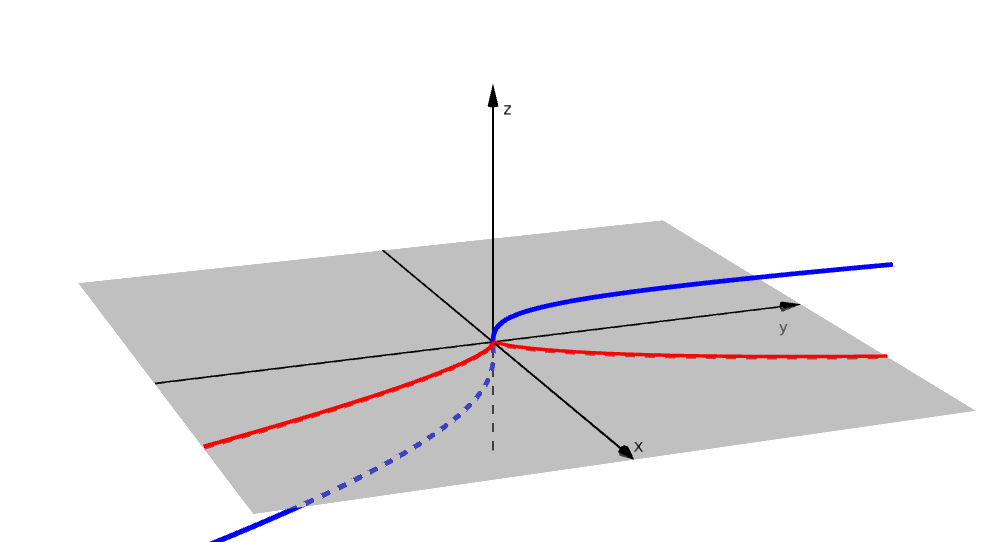
\includegraphics[width=10cm]{cuspidal-resol.png}
\end{center}

\begin{ejercicio}
  Consideremos las $k$-álgebras
  $$A \dfn k [x,y]/(x^2\,(x+1)-y^2), \quad B \dfn k[x,y,z]/(x-z^2+1, y-z^3+z).$$
  Demuestre que se tiene un homomorfismo inyectivo natural
  $A \hookrightarrow B$, y $B$ es integral sobre $A$.
\end{ejercicio}

Al homomorfismo $A \hookrightarrow B$ del ejercicio anterior corresponde
la proyección natural entre los conjuntos algebraicos
$$\mathbf{V} (x-z^2+1, y-z^3+z) \subset \AA^3 (k) \quad\text{y}\quad \mathbf{V} (x^2\,(x+1)-y^2) \subset \AA^2 (k).$$

\begin{center}
  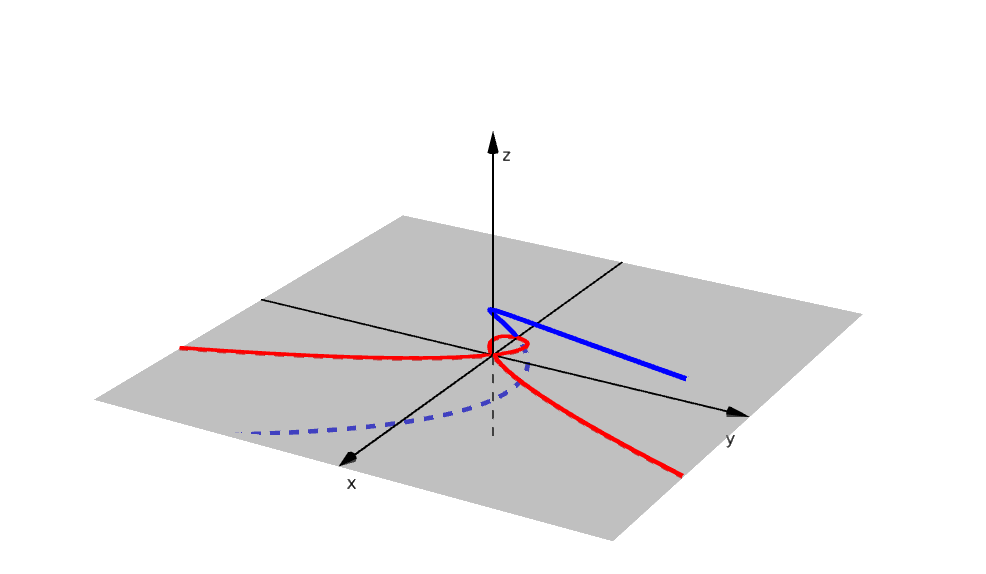
\includegraphics[width=10cm]{nodal-resol.png}
\end{center}

\subsection{Normalización de Noether}

Como hemos visto en el teorema \ref{thm:dim-y-trdeg}, si $A$ es una $k$-álgebra
finitamente generada de dimensión $d$, entonces existen elementos
algebraicamente independientes $a_1,\ldots,a_d \in A$. El siguiente resultado
nos dice que estos elementos pueden ser escogidos de tal manera que
$k [a_1,\ldots,a_d] \subseteq A$ es una extensión integral.

\begin{nameless}\textbf{Teorema de normalización de Noether.}
  \label{thm:normalizacion-de-noether}
  \emph{Sea $A = k[x_1,\ldots,x_n]/I$ una $k$-álgebra finitamente generada no
    nula. Entonces, existen elementos
    $$a_1,\ldots,a_d\in A$$
    tales que
    \begin{enumerate}
    \item[1)] $a_1,\ldots,a_d$ son algebraicamente independientes sobre $k$;
    \item[2)] $A$ es una extensión integral de $k [a_1,\ldots,a_d]$;
    \item[3)] $A$ es finitamente generado como un módulo sobre
      $k [a_1,\ldots,a_d]$;
    \item[4)] $d = \dim A$.
    \end{enumerate}}
\end{nameless}

Antes de lanzarnos en la prueba, expliquemos cuál es el punto de lo que vamos
a hacer. En el ejemplo \ref{ejemplo:normalizacion-de-cubica-nodal} de arriba
teníamos $A = k [x,y]/(x^3-y^2)$, y allí es fácil ver que $A$ es integral sobre
$k [\overline{x}]$ y también sobre $k [\overline{y}]$: tenemos una relación
integral de $\overline{y}$ sobre $k [\overline{x}]$ dada por
$\overline{y}^2 - \overline{x}^3 = 0$, y de la misma manera una relación
integral de $\overline{x}$ sobre $k [\overline{y}]$. Sin embargo, no es siempre
posible obtener una dependencia integral directamente. Por ejemplo, en el caso
de $A = k [x_1,x_2]/(x_1 x_2 - 1)$, el polinomio $f = x_1 x_2 - 1$ no nos da una
dependencia integral de $\overline{x_2}$ sobre $k [\overline{x_1}]$, ni de
$\overline{x_1}$ sobre $k [\overline{x_2}]$ (de hecho, tales dependencias
integrales simplemente no existen). La siguiente prueba consiste en un truco que
permite sustituir $x_2$ por otra expresión $y_2$ en $x_1 x_2 - 1$ para poder
sacar una dependencia integral de $x_1$ sobre $k [\overline{y_2}] \subseteq A$.

\begin{proof}
  Procedamos por inducción sobre $n$. La base de inducción es el caso cuando
  $n = 0$. Para el paso inductivo, notamos que si $I = 0$, entonces bastaría
  tomar $a_i = x_i$ para $i = 1,\ldots,n$. Asumamos entonces que
  $0 \ne I \subsetneq A$. Todo polinomio no nulo $f \in I$ puede ser escrito
  como
  $$f = \sum_{(i_1,\ldots,i_n) \in S} c_{i_1,\ldots,i_n}\,x_1^{i_1}\cdots x_n^{i_n},$$
  donde $S \subseteq \NN^n$ es un conjunto finito no vacío. Escojamos
  $\delta > \deg f$ y pongamos
  $$y_i \dfn x_i - x_1^{\delta^{i-1}}, \quad i = 2,\ldots,n.$$
  Ahora
  $$f = f (x_1, y_2 + x_1^\delta, y_3 + x_1^{\delta^2}, \ldots, y_n + x_1^{\delta^{n-1}}) = \sum_{(i_1,\ldots,i_n) \in S} c_{i_1,\ldots,i_n}\,\left(x_1^{s (i_1,\ldots,i_n)} + g_{i_1,\ldots,i_n} (x_1,y_2,\ldots,y_n) \right),$$
  donde
  $$s (i_1,\ldots,i_n) \dfn i_1 + i_2\,\delta + i_3\,\delta^2 + \cdots + i_n\,\delta^{n-1},$$
  y los polinomios $g_{i_1,\ldots,i_n}$ cumplen
  $$\deg_{x_1} (g_{i_1,\ldots,i_n}) < s (i_1,\ldots,i_n).$$
  Notamos que la función
  $$(i_1,\ldots,i_n) \mapsto s (i_1,\ldots,i_n)$$
  es inyectiva sobre $S$ por nuestra elección de $\delta$, y por ende existe
  único $(i_1,\ldots,i_n) \in S$ tal que el valor $N \dfn s (i_1,\ldots,i_n)$ es
  el máximo posible. El polinomio $f$ no es constante, así que $N > 0$. Podemos
  escribir
  $$f = c_{i_1,\ldots,i_n}\,x_1^N + h (x_1,y_2,\ldots,y_n),$$
  donde $\deg_{x_1} (h) < N$. Luego,
  \begin{equation}
    \label{eqn:noether-relacion-para-x1}
    x_1^N + c_{i_1,\ldots,i_n}^{-1}\,h (x_1,y_2,\ldots,y_n) \in I.
  \end{equation}
  Consideremos la $k$-álgebra
  $$C \dfn k [\overline{y_2}, \ldots, \overline{y_n}] \subseteq A.$$
  Tenemos
  $$A = C [\overline{x_1}],$$
  donde $\overline{x_1}$ es un elemento integral sobre $A$ gracias a la relación
  \eqnref{eqn:noether-relacion-para-x1}. Esto implica también que $A$ es un
  módulo finitamente generado sobre $C$ (véase el lema
  \ref{lema:integralidad-y-modulos-fg}). Entonces, $A$ es integral sobre
  $C$. Ahora por inducción, existen elementos $b_1,\ldots,b_d \in C$
  algebraicamente independientes sobre $k$ tales que $C$ es integral sobre
  $k [b_1,\ldots,b_d]$ y es un módulo finitamente generado sobre
  $k [b_1,\ldots,b_d]$. Luego, $A$ cumple las mismas propiedades sobre
  $k [b_1,\ldots,b_d]$ (véase el lema
  \ref{lema:cadena-de-extensiones-integrales}).

  Notamos que si $a_1,\ldots,a_d$ son algebraicamente independientes, entonces
  $$\dim k [a_1,\ldots,a_d] = \dim k [x_1,\ldots,x_d] = d.$$
  Ahora si $A$ es integral sobre $k [a_1,\ldots,a_d]$, entonces
  $$\dim A = \dim k [a_1,\ldots,a_d] = d$$
  gracias al lema \ref{lema:extensiones-integrales-dimension}.
\end{proof}

La prueba de arriba es constructiva y contiene un algoritmo para obtener los
elementos $a_1,\ldots,a_d \in A$.

\begin{ejemplo}
  Consideremos $A = k[x_1,x_2]/(x_1 x_2 - 1)$. La prueba del teorema de arriba
  nos sugiere considerar el polinomio
  $$f = x_1 x_2 - 1.$$
  Este tiene grado $2$, así que podemos poner $\delta = 3$ y
  $$y_2 \dfn x_2 - x_1^3.$$
  Ahora
  $$f = x_1\,(x_1^3 + y_2) = x_1^4 + x_1 y_2.$$
  Esto demuestra que $\overline{x_1} \in A$ es integral sobre
  $C \dfn k [\overline{y_2}] \isom k [t]$. Entonces, nuestra prueba de
  la normalización de Noether nos dice que $A$ es integral sobre $k [a]$,
  donde $a = \overline{x_2} - \overline{x_1}^4$. Luego,
  $$k [\overline{x_2} - \overline{x_1}^4] \isom k [t]/\ker\phi,$$
  donde
  $$\phi\colon k [t] \to k [x_1,x_2]/(x_1 x_2 - 1), \quad t \mapsto \overline{x_2 - x_1^4}.$$
  Uno puede comprobar que este homomorfismo es inyectivo:
  $$\ker \phi = (x_1 x_2 - 1, \, x_2 - x_1^4 - t) \cap k [t] = (0),$$
  así que
  \[ k [\overline{x_2} - \overline{x_1}^4] \isom k [t]. \qedhere \]
\end{ejemplo}

El elemento $x_2 - x_1^4$ que surgió en el último ejemplo es algo aleatorio,
y de hecho la normalización de Noether tiene otra prueba más natural que vamos
a ver a continuación.

\subsection{Normalización de Noether: forma lineal}

\begin{ejemplo}
  Continuando el ejemplo de $A = k [x_1,x_2]/(x_1 x_2 - 1)$, notamos que las
  extensiones ${k [\overline{x_1}] \subset A}$ y
  ${k [\overline{x_2}] \subset A}$ \emph{no son} integrales. He aquí un modo
  geométrico de verlo. Por ejemplo, si la extensión
  $k [\overline{x_1}] \subset A$ fuera integral, entonces por el teorema de
  Cohen--Seidenberg habría un ideal primo $\mathfrak{p} \subset A$ tal que
  $\mathfrak{p} \cap k [\overline{x_1}] = (\overline{x_1})$. Pero
  $\overline{x_1}$ es invertible en $A$, su inverso siendo $\overline{x_2}$,
  así que sobre el ideal primo $(\overline{x_1}) \subset k [\overline{x_1}]$ no
  puede haber ningún primo en $A$.

  De hecho, la inclusión $k [\overline{x_1}] \subset A$ corresponde a la
  proyección
  \begin{align*}
    \phi\colon \mathbf{V} (x_1 x_2 - 1) & \to \AA^1 (k),\\
    (t,t^{-1}) & \mapsto t,
  \end{align*}
  y el problema es que el punto $0$ no está en la imagen de $\phi$.

  Podemos tomar la proyección ortogonal sobre la recta $x_1 + x_2 = 0$. Cuando
  $\fchar k \ne 2$, tal proyección se define mediante el morfismo
  \begin{align*}
    \mathbf{V} (x_1 x_2 - 1) & \to \AA^2 (k)/(x_1+x_2),\\
    (x_1,x_2) & \mapsto \left(\frac{x_1-x_2}{2}, \frac{x_2-x_1}{2}\right).
  \end{align*}

  \begin{center}
    \begin{tikzpicture}[x=1cm, y=1cm]

      \draw[domain=-3.2:-1/(3.2),smooth,variable=\t] plot ({\t},{1/\t});
      \draw[domain=1/(3.2):(3.2),smooth,variable=\t] plot ({\t},{1/\t});

      \draw (-2,2) -- (2,-2) node[below right] {$x_1+x_2 = 0$};

      \foreach \i in {1,...,3}
        \draw[dashed] (1/\i,\i) -- ({-\i,-1/\i});
      \foreach \i in {2,...,3}
        \draw[dashed] (\i,1/\i) -- ({-1/\i,-\i});

      \iffalse
      \draw[dashed] (1,1) -- ({(1-1)/2},{(1-1)/2});
      \draw[dashed] (2,1/2) -- ({(2-1/2)/2},{(1/2-2)/2});
      \draw[dashed] (3,1/3) -- ({(3-1/3)/2},{(1/3-3)/2});
      \draw[dashed] (1/2,2) -- ({(1/2-2)/2},{(2-1/2)/2});
      \draw[dashed] (1/3,3) -- ({(1/3-3)/2},{(3-1/3)/2});
      \draw[dashed] (-1,-1) -- ({(-1+1)/2},{(-1+1)/2});
      \draw[dashed] (-2,-1/2) -- ({(-2+1/2)/2},{(-1/2+2)/2});
      \draw[dashed] (-3,-1/3) -- ({(-3+1/3)/2},{(-1/3+3)/2});
      \draw[dashed] (-1/2,-2) -- ({(-1/2+2)/2},{(-2+1/2)/2});
      \draw[dashed] (-1/3,-3) -- ({(-1/3+3)/2},{(-3+1/3)/2});
      \fi

      \draw[->] (-3,0) -- (3,0) node[right] {$x_1$};
      \draw[->] (0,-3) -- (0,3) node[above] {$x_2$};
    \end{tikzpicture}
  \end{center}

  Si nos preocupa la característica $2$, podemos tomar el morfismo
  $$(x,y) \mapsto \left(x_1-x_2, x_2-x_1\right).$$
  Tenemos el homomorfismo correspondiente
  $$k [t] \xrightarrow{\isom} k [x_1,x_2]/(x_1 + x_2) \to k [x_1,x_2]/(x_1\,x_2 - 1),$$
  donde $t \mapsto x_1$. La imagen de este homomorfismo es
  $k [\overline{x_1} - \overline{x_2}] \subset A$. Notamos que $A$ es integral
  sobre $k [\overline{x_1} - \overline{x_2}]$ gracias a las relaciones
  \[ \overline{x_1}^2 - (\overline{x_1}-\overline{x_2})\,\overline{x_1} - 1 = \overline{x_2}^2 + (\overline{x_1}-\overline{x_2})\,\overline{x_2} - 1 = 0. \qedhere \]
\end{ejemplo}

El último ejemplo sugiere que la normalización de Noether puede ser mejorada de
la siguiente manera.

\begin{teorema}
  Asumamos que el cuerpo base $k$ es infinito. Sea $A = k[x_1,\ldots,x_n]/I$ una
  $k$-álgebra finitamente generada no nula. Entonces, existen $n$ elementos
  $$a_1,\ldots,a_d \in A$$
  que cumplen las condiciones del teorema de normalización de Noether y que
  pueden ser elegidos como combinaciones lineales
  $$a_i = x_i + \sum_{d+1 \le j \le n} c_{i,j}\,x_j$$
  para algunos $c_{i,j} \in k$.

  \begin{proof}
    Vamos a seguir la prueba de \ref{thm:normalizacion-de-noether}, solo
    necesitamos modificar un poco el paso inductivo. Consideremos un polinomio
    no nulo
    $$f = \sum_{(i_1,\ldots,i_n) \in S} c_{i_1,\ldots,i_n}\,x_1^{i_1}\cdots x_n^{i_n} \in I.$$
    Pongamos
    $$y_i \dfn x_i - c_i\,x_n\quad\text{para }i = 1,\ldots,n-1$$
    para algunos $c_i \in k$ (que vamos a escoger más adelante). Ahora
    $$f = f (y_1+c_1\,x_n, y_2+c_2\,x_n, \ldots, x_n) = \sum_{(i_1,\ldots,i_n) \in S} c_{i_1,\ldots,i_n}\,\left(c_1^{i_1}\cdots c_{n-1}^{i_{n-1}}\,x_n^{s (i_1,\ldots,i_n)} + g_{i_1,\ldots,i_n} (y_1,y_2,\ldots,x_n)\right),$$
    donde
    $$s (i_1,\ldots,i_n) \dfn i_1 + i_2 + \cdots + i_n,$$
    y los polinomios $g_{i_1,\ldots,i_n}$ cumplen
    $$\deg_{x_n} (g_{i_1,\ldots,i_n}) < s (i_1,\ldots,i_n).$$
    Sea $f_d \in k [x_1,\ldots,x_n]$ la parte homogénea de $f$ de grado
    $d \dfn \deg f$. Tenemos entonces
    $$f = f_d (c_1,\ldots,c_{n-1},1)\cdot x_n^d + h (y_1,\ldots,y_{n-1},x_n),$$
    donde $\deg_{x_n} (h) < d$. Ahora dado que el cuerpo $k$ es infinito (!),
    podemos escoger algunos elementos ${c_1,\ldots,c_{n-1} \in k}$ de tal manera
    que $f_d (c_1,\ldots,c_{n-1},1) \ne 0$. En este caso la identidad de arriba
    nos dirá que $\overline{x_n}$ es integral sobre la subálgebra
    $$C \dfn k [\overline{y_1}, \ldots, \overline{y_{n-1}}].$$
    Luego, $A = C [\overline{x_n}]$ es integral sobre $C$.
  \end{proof}
\end{teorema}

\begin{ejemplo}
  Volvamos al álgebra $A = k [x_1,x_2] / (x_1 x_2 - 1)$ para entender cómo
  funciona el argumento de arriba. Podemos considerar el polinomio
  $$f = x_1 x_2 - 1$$
  y hacer una sustitución lineal $y_1 = x_1 - cx_2$. Luego,
  $$f (x_1,x_2) = f (y_1 + cx_2, x_2) = (y_1 + cx_2)\,x_2 - 1 = cx_2^2 + y_1 x_2 - 1.$$
  Entonces, para obtener una dependencia integral de $\overline{x_2}$ sobre
  $k [\overline{y}_1]$, basta tomar cualquier $c \ne 0$. En particular, podemos
  considerar $c = -1$, lo que nos dirá que $A$ es integral sobre
  $k [\overline{y}_1] = k [\overline{x_1} + \overline{x_2}]$.
\end{ejemplo}

\begin{ejemplo}
  \label{ejemplo:normalizacion-lineal-F2}
  La hipótesis que el cuerpo $k$ es infinito es importante. Consideremos por
  ejemplo
  $$A = k [x_1,x_2]/(x_1^2\,x_2 + x_1\,x_2^2 + 1).$$
  En este caso $\overline{x_1}$, $\overline{x_2}$,
  $\overline{x_1} + \overline{x_2}$ son invertibles en $A$:
  \begin{align*}
    \overline{x_1}^{-1} & = -(\overline{x_1}\,\overline{x_2} + \overline{x_2}^2),\\
    \overline{x_2}^{-1} & = -(\overline{x_1}\,\overline{x_2} + \overline{x_1}^2),\\
    (\overline{x_1} + \overline{x_2})^{-1} & = -\overline{x_1}\,\overline{x_2}.
  \end{align*}
  Esto significa que $A$ no puede ser integral sobre las subálgebras
  $k [\overline{x_1}]$, $k [\overline{x_2}]$,
  $k [\overline{x_1} + \overline{x_2}]$. Ahora si $k = \FF_2$, entonces
  las únicas combinaciones lineales no triviales de $\overline{x_1}$ y
  $\overline{x_2}$ son estas tres, y la normalización de Noether en la forma
  lineal no existe.

  \begin{center}
    \begin{tikzpicture}[x=1cm, y=1cm]

      \draw[domain=-3:-0.1,smooth,variable=\t] plot ({\t},{(-sqrt(\t*\t*\t*\t-4*\t)-\t*\t)/(2*\t)});
      \draw[domain=-3:-0.1,smooth,variable=\t] plot ({\t},{(sqrt(\t*\t*\t*\t-4*\t)-\t*\t)/(2*\t)});

      \draw[domain=1.5875:3,smooth,variable=\t] plot ({\t},{(-sqrt(\t*\t*\t*\t-4*\t)-\t*\t)/(2*\t)});
      \draw[domain=1.5875:3,smooth,variable=\t] plot ({\t},{(sqrt(\t*\t*\t*\t-4*\t)-\t*\t)/(2*\t)});

      \draw[dashed] (-3,3) -- (3,-3);
      % \draw[dashed] (-3,-3) -- (3,3);

      \draw[->] (-3.2,0) -- (3.2,0) node[right] {$x_1$};
      \draw[->] (0,-3.4) -- (0,3.4) node[above] {$x_2$};
    \end{tikzpicture}
  \end{center}

  Nuestra prueba de arriba no va a funcionar porque para
  $$f = x_1^2 x_2 + x_1 x_2^2 + 1$$
  la parte homogénea de grado mayor será
  $$f_2 = x_1^2 x_2 + x_1 x_2^2,$$
  y este polinomio se anula en todo $x_1,x_2 \in \FF_2$.
\end{ejemplo}

Sin entrar en los detalles (\emph{lamentablemente}, este no es precisamente un
curso de geometría algebraica), la normalización de Noether en la forma
establecida arriba significa que para $k$ algebraicamente cerrado, un conjunto
algebraico $\mathbf{V} (f) \subset \AA^n (k)$ puede ser proyectado a algún
hiperplano $H \subset \AA^n (k)$ de tal manera que para todo punto $x \in H$ la
preimagen $p^{-1} (x)$ es finita y no vacía.

\begin{ejercicio}
  Consideremos la $k$-álgebra
  $A \dfn k [x_1,x_2] / (x_1 x_2^2 + x_1^2 x_2 + 1)$. Encuentre

  \begin{enumerate}
  \item[a)] una normalización de Noether para $k = \FF_2$ (recuerde que esta no
    puede ser lineal),

  \item[b)] una normalización de Noether para $k = \QQ$ de la forma
    $a = c_1 x_1 + c_2 x_2$ para $c_1, c_2 \in \QQ$.
  \end{enumerate}
\end{ejercicio}

\begin{ejercicio}
  Encuentre una normalización de Noether en la forma lineal para la $k$-álgebra
  $$A \dfn k [x_1,x_2,x_3] / (x_1^2 x_2^2, \, x_1^2 x_3^2).$$
\end{ejercicio}

\subsection{Normalización de Noether en \Mac{}}

Para calcular la normalización de Noether en \Mac{}, existe el paquete
\texttt{NoetherNormalization}. Para usarlo, primero hay que ejecutar el comando
\begin{center}
  \texttt{loadPackage "NoetherNormalization";}
\end{center}
Este paquete provee la función \texttt{noetherNormalization\,($I$)} o
\texttt{noetherNormalization\,($k[x_1,\ldots,x_n]/I$)} que calcula una
normalización de Noether para $k[x_1,\ldots,x_n]/I$. A saber, para encontrarla,
se busca un \emph{automorfismo lineal}
\begin{align*}
  \phi\colon k[x_1,\ldots,x_n] & \to k[x_1,\ldots,x_n],\\
  x_i & \mapsto \sum_j c_{ij}\,x_j
\end{align*}
y variables $x_{i_1}, \ldots, x_{i_d}$ tales que son algebraicamente
independientes y $k [x_1,\ldots,x_n]/\phi (I)$ es integral sobre la subálgebra
$k [\overline{x_{i_1}}, \ldots, \overline{x_{i_d}}]$. Los coeficientes $c_{ij}$
se buscan de modo aleatorio, y como hemos visto arriba, esto en general no
funciona si $k$ es un cuerpo finito.

\iffalse
\begin{ejemplo}
  Calculemos una normalización de $\QQ[x,y,z]/(x^2+y^2-z^2)$.

  \begin{framed}\footnotesize
\begin{verbatim}
i1 : loadPackage "NoetherNormalization";

i2 : noetherNormalization (QQ[x,y,z]/(x^2+y^2-z^2))

                                                     2    2    2
o2 = (map(QQ[x, y, z],QQ[x, y, z],{x, z, y}), ideal(x  - y  + z ), {z, y})

o2 : Sequence
\end{verbatim}
  \end{framed}

  Aquí la salida de
  \texttt{noetherNormalization\,(QQ[x,y,z]/(x\^{}2+y\^{}2-z\^{}2))} consiste en
  tres elementos.

  \begin{enumerate}
  \item[1)] Un automorfismo del anillo $\QQ [x,y,z]$ dado por
    $$\phi\colon x \mapsto x, \quad y \mapsto z, \quad z \mapsto y.$$

  \item[2)] El ideal $J = (x^2 - y^2 + z^2)$ que es la imagen de
    $I = (x^2 + y^2 - z^2)$ respecto al automorfismo $\phi$.

  \item[3)] Una lista de variables $(x_1,\ldots,x_d)$ (en este caso $z$ e $y$)
    tales que $\overline{x_1}, \ldots, \overline{x_d}$ son algebraicamente
    independientes en $R/J$ y $R/J$ es integral sobre
    $k [\overline{x_1}, \ldots, \overline{x_d}]$.
  \end{enumerate}
\end{ejemplo}
\fi

\begin{ejemplo}
  Calculemos una normalización de Noether de $\QQ [x,y] / (x^3 - y^2)$ (ejemplo
  \ref{ejemplo:normalizacion-de-cubica-nodal}).

  \begin{framed}\footnotesize
\begin{verbatim}
i : noetherNormalization (QQ[x,y]/(x^3-y^2))

                                           3    2
o = (map(QQ[x, y],QQ[x, y],{x, y}), ideal(x  - y ), {y})

o : Sequence
\end{verbatim}
  \end{framed}

  Notamos que el automorfismo $\phi$ en este caso es la aplicación identidad.
\end{ejemplo}

\begin{ejemplo}
  Tratemos de calcular una normalización de Noether de
  $k[x,y]/(x^2y + xy^2 + 1)$ (ejemplo \ref{ejemplo:normalizacion-lineal-F2})
  para $k = \FF_2$ y $\FF_3$.

  \begin{framed}\footnotesize
\begin{verbatim}
i : noetherNormalization (ZZ/2[x,y]/(x^2*y + x*y^2 + 1))
--warning: no good linear transformation found by noetherNormalization

         ZZ       ZZ                           2       2
o = (map(--[x, y],--[x, y],{x + y, x}), ideal(x y + x*y  + 1), {y})
          2        2

o : Sequence

i : noetherNormalization (ZZ/3[x,y]/(x^2*y + x*y^2 + 1))

         ZZ       ZZ                             3      2
o = (map(--[x, y],--[x, y],{x + y, x}), ideal(- x  + x*y  + 1), {y})
          3        3

o : Sequence
\end{verbatim}
  \end{framed}

  Aquí primero \Mac{} nos avisa que una normalización no fue encontrada en
  el caso de $k = \FF_2$. Esto sucede porque \texttt{noetherNormalization}
  analiza combinaciones lineales de las variables, lo que no puede funcionar
  en este caso particular (véase el ejemplo
  \ref{ejemplo:normalizacion-lineal-F2}).

  Para $k = \FF_3$ fue encontrado el automorfismo
  $$\phi\colon x \mapsto x+y, \quad y \mapsto x$$
  y una normalización de Noether de
  $$k [x,y]/I \isom k [x,y]/\phi (I) = k [x,y]/(x^3 - xy^2 - 1):$$
  la salida significa que el álgebra $k [x,y]/(x^3 - xy^2 - 1)$ es integral
  sobre $k [\overline{y}]$. En efecto, se tiene la relación
  $$\overline{x}^3 - \overline{x}\,\overline{y}^2 - 1 = 0\text{ en }k [x,y]/(x^3 - xy^2 - 1).$$
  Notamos que $\phi^{-1} (x) = y$, $\phi^{-1} (y) = x-y$, así que en términos
  de $k [x,y]/I$, lo que fue calculado significa que
  $k [\overline{x},\overline{y}] = k [\overline{y},\overline{x}-\overline{y}]$
  es integral sobre la subálgebra $k [\overline{x}-\overline{y}]$, puesto que
  \[ \overline{y}^3 - \overline{y}\,(\overline{x}-\overline{y})^2 - 1 = 0\text{ en }k[x,y]/(x^2y + xy^2 + 1). \qedhere \]
\end{ejemplo}

\begin{comentario}
  No hay que confundir \term{una normalización de Noether} de $A$ con la noción
  de \term{la cerradura integral}\footnote{Si tuviera más tiempo,
    definitivamente hablaría de la cerradura integral y su cálculo.}, que a
  veces también se conoce como \term{la normalización}. Para una $R$-álgebra $A$
  que es un dominio, se pueden considerar los elementos de $\Frac A$ integrales
  sobre $A$. Estos forman una $R$-subálgebra $\widetilde{A} \subset \Frac A$ que
  se llama la \term{cerradura integral} de $A$. Cuando $A = \widetilde{A}$,
  se dice que $A$ es \term{integralmente cerrada} o \term{normal}.

  Por ejemplo, el álgebra $A = k [x,y]/(x^3-y^2)$ no es integralmente cerrada,
  y su cerradura integral fue descrita en
  \ref{ejemplo:normalizacion-de-cubica-nodal}. La importancia geométrica de este
  concepto se refleja en el hecho de que para una curva $C$, el álgebra
  $\Gamma (C)$ es integralmente cerrada si y solo si $C$ no tiene
  singularidades. La curva $y^2 = x^3$ tiene una cúspide en el origen, mientras
  que la cúbica torcida ``resuleve'' esta singularidad.

  Para calcular la cerradura integral en \Mac{}, existe la función
  \texttt{integralClosure}. He aquí un pequeño ejemplo:

  \begin{framed}\footnotesize
\begin{verbatim}
i : integralClosure (QQ[x,y]/(x^3-y^2))

              QQ[w   , x, y]
                  0,0
o = ---------------------------------
              2              2
    (w   y - x , w   x - y, w    - x)
      0,0         0,0        0,0

o : QuotientRing
\end{verbatim}
  \end{framed}

  Aquí la salida es la $\QQ$-álgebra
  $$\QQ [w, x, y] / (w y - x^2, \, w x - y, \, w^2 - x).$$
  Notamos que
  $$(w y - x^2, \, w x - y, \, w^2 - x) = (x-w^2, \, y-w^3),$$
  así que \Mac{} encontró la cúbica torcida (véase el ejemplo
  \ref{ejemplo:normalizacion-de-cubica-nodal}).
\end{comentario}

% % % % % % % % % % % % % % % % % % % % % % % % % % % % % %

\section{Series de Hilbert y dimensión}

Volvamos al estudio de la serie y polinomio de Hilbert. He aquí una pequeña
tabla de ideales y sus series y polinomios de Hilbert.

\begin{center}
\begin{tabular}{f{6cm}f{5.25cm}f{2cm}f{1.25cm}}
\hline
$I$ & $H_I (t)$ & $p_I (x)$ & $\dim A$ \tabularnewline
\hline
$(0) \subset k [x_1,\ldots,x_n]$ & $\frac{1}{(1-t)^n} = \sum\limits_{d \ge 0} {d + n - 1 \choose n-1}\,t^d$ & ${x + n - 1 \choose n-1}$ & $n$ \tabularnewline
\hline
$(x^4+y^4+z^4+w^4) \subset k [x,y,z,w]$ & $\frac{1-t^4}{(1-t)^4} = \frac{t^3 + t^2 + t + 1}{(1-t)^3}$

$= 1 + 4t + 10t^2 + 20t^3 + 34t^4 + \cdots$ & $2x^2+2$ & $3$ \tabularnewline
\hline
$(xz,yz) \subset k [x,y,z]$ & $\frac{t^3 - 2 t^2 + 1}{(1-t)^3} = \frac{-t^2+t+1}{(1-t)^2}$

$= 1 + 3t + 4t^2 + 5t^3 + 6t^4 + \cdots$ & $x+2$ & $2$ \tabularnewline
\hline
$(x^2+y^2-z^2) \subset k [x,y,z]$ & $\frac{-t^2 + 1}{(1-t)^3} = \frac{1+t}{(1-t)^2}$

$= 1 + 3 t + 5 t^2 + 7 t^3 + 9 t^4 + \cdots$ & $2x+1$ & $2$ \tabularnewline
\hline
$(x^2-y) \subset k [x,y]$ & $\frac{-t^2 + 1}{(1-t)^2} = \frac{1+t}{1-t}$

$= 1 + 2 t + 2 t^2 + 2 t^3 + 2 t^4 + \cdots$ & $2$ & $1$ \tabularnewline
\hline
$(x^2 - y, \, x^3 - z) \subset k [x,y,z]$ & $\frac{2t^3 - 3 t^2 + 1}{(1-t)^3} = \frac{2t+1}{1-t}$

$= 1 + 3 t + 3 t^2 + 3 t^3 + 3 t^4 + \cdots$ & $3$ & $1$
\tabularnewline
\hline
\end{tabular}
\end{center}

Se nota que
$$\dim (k [x_1,\ldots,x_n]/I) = \deg p_I + 1,$$
y que la dimensión es el mínimo número $\delta$ tal que la serie de Hilbert
puede ser escrita como
$$H_I (t) = \frac{f (t)}{(1-t)^\delta},$$
donde $f (t) \in \ZZ [t]$. La minimalidad de $\delta$ significa que
$f (1) \ne 0$ (sino, $f (t)$ tendría un factor $(1-t)$). Primero aclaramos la
relación entre $\delta$ y el grado del polinomio de Hilbert.

\begin{proposicion}
  Para un ideal $I \subset k [x_1,\ldots,x_n]$, sea $\delta$ el número tal que
  la serie de Hilbert puede ser escrita como
  $$H_I (t) = \frac{f (t)}{(1-t)^\delta},$$
  donde $f (1) \ne 0$. Entonces,
  $$\delta = \deg p_I + 1.$$

  \begin{proof}
    Escribamos
    $$H_I (t) = \frac{f (t)}{(1-t)^\delta} = \frac{a_m\,t^m + \cdots + a_1\,t + a_0}{(1-t)^\delta},$$
    donde $f (1) \ne 0$. Ahora como en la prueba de
    \ref{cor:polinomio-y-funcion-de-Hilbert}, podemos expresar el polinomio de
    Hilbert mediante
    $$p_I = \sum_{0 \le i \le m} a_i {x - i + \delta - 1 \choose \delta-1}.$$
    Notamos que
    $${x - i + \delta - 1 \choose \delta-1} = \frac{x^{\delta-1}}{(\delta-1)!} + \cdots.$$
    Esto significa que $\deg p_I \le \delta-1$. Por otra parte, el coeficiente
    de $x^{\delta-1}$ del polinomio $p_I$ es igual a
    $$\sum_{0 \le i \le m} \frac{a_i}{(\delta-1)!} = \frac{f (1)}{(\delta-1)!} \ne 0.$$
    Podemos concluir que $\deg p_I = \delta-1$.
  \end{proof}
\end{proposicion}

Recordemos que el polinomio de Hilbert se caracteriza por
$$p_I (d) = h_I (d)\quad\text{para }d \gg 0.$$
En algunos cálculos ya hemos ocupado la función de Hilbert alternativa
$$\widetilde{h}_I (d) \dfn \dim_k (k [x_1,\ldots,x_n]/I)_{\le d} = \{ \overline{f} \mid f \in k [x_1,\ldots,x_n], \, \deg f \le d \}.$$
Tenemos
$$h_I (d) = \widetilde{h}_I (d) - \widetilde{h}_I (d-1).$$
Sería conveniente trabajar con otro polinomio de Hilbert caracterizado por
$$\widetilde{p}_I (d) = \widetilde{h}_I (d)\quad\text{para }d \gg 0.$$
Tenemos entonces
$$p_I (x) = \widetilde{p}_I (x) - \widetilde{p}_I (x-1).$$
Notamos que si $\widetilde{p}_I (x) = c_m\,x^m + \cdots$, entonces
$$\widetilde{p}_I (x) - \widetilde{p}_I (x-1) = m\,c_m\,x^{m-1} + \cdots,$$
así que
$$\deg \widetilde{p}_I (x) = \deg p_I (x)+1.$$
A partir de ahora nuestro objetivo será probar que
$$\delta = \deg p_I (x)+1 = \deg \widetilde{p}_I (x) \stackrel{???}{=} \dim (k [x_1,\ldots,x_n]/I).$$

\begin{lema}
  Supongamos que para dos ideales
  $$I \subseteq k [x_1,\ldots,x_m] \quad\text{y}\quad J \subseteq k [y_1,\ldots,y_n]$$
  se tiene
  $$k [x_1,\ldots,x_m]/I \isom k [y_1,\ldots,y_n]/J.$$
  Luego,
  $$\deg \widetilde{p}_I = \deg \widetilde{p}_J.$$

  \begin{proof}
    Consideremos un isomorfismo de $k$-álgebras
    $$\phi\colon k [x_1,\ldots,x_m]/I \xrightarrow{\isom} k [y_1,\ldots,y_n]/J.$$
    Entonces, existen polinomios $f_1,\ldots,f_n \in k [x_1,\ldots,x_m]$ tales
    que $\phi (\overline{f_i}) = \overline{y_i}$. Pongamos
    $$N \dfn \max \{ \deg f_1, \ldots, \deg f_n \}.$$
    Luego, para todo $d$ se tiene
    $$(k [y_1,\ldots,y_n]/J)_{\le d} \subseteq \phi \Bigl((k [x_1,\ldots,x_m]/I)_{\le Nd}\Bigr).$$
    Esto nos da la desigualdad $\widetilde{h}_J (d) \le \widetilde{h}_I (Nd)$, y
    luego
    $$\widetilde{p}_J (d) \le \widetilde{p}_I (Nd)\quad\text{para }d \gg 0.$$
    Esto implica que $\deg \widetilde{p}_J \le \deg \widetilde{p}_I$. De la
    misma manera se obtiene la otra desigualdad
    $\deg \widetilde{p}_I \le \deg \widetilde{p}_J$.
  \end{proof}
\end{lema}

\begin{teorema}
  Para toda $k$-álgebra finitamente generada $A \dfn k [x_1,\ldots,x_n]/I$ se
  tiene
  $$\dim A = \deg \widetilde{p}_I.$$

  \begin{proof}
    Podemos asumir que $A\ne 0$; en el caso contrario la identidad se cumple por
    las convenciones sobre $\dim 0$ y $\deg 0$. La normalización de Noether nos
    da elementos $a_1,\ldots,a_\delta \in A$ tales que la extensión
    $$C \dfn k [a_1,\ldots,a_\delta] \subseteq A$$
    es integral, $\delta = \dim A$, y además $A$ es un $C$-módulo finitamente
    generado. Lo último significa que existen elementos $b_1,\ldots,b_r \in A$
    tales que
    $$A = C\cdot b_1 + \cdots + C\cdot b_r.$$
    Podemos asumir que $b_1 = 1$ y otros elementos $b_2,\ldots,b_r$ están
    representados por polinomios de grado $> 0$. Consideremos el homomorfismo de
    $k$-álgebras
    \begin{align*}
      \phi\colon k [y_1,\ldots,y_\delta, \, z_1,\ldots,z_r] & \to A,\\
      y_i & \mapsto a_i,\\
      z_j & \mapsto b_j.
    \end{align*}
    Puesto que $\phi$ es sobreyectivo,
    $$A = k [x_1,\ldots,x_n]/I \isom k [y_1,\ldots,y_\delta, \, z_1,\ldots,z_r]/J, \quad \text{donde }J = \ker\phi.$$
    Por el lema anterior, tenemos entonces
    $\deg \widetilde{p}_I = \deg \widetilde{p}_J$, y nuestro objetivo será
    probar que $\deg \widetilde{p}_J = \delta$.

    Recordemos que $\widetilde{h}_J (d)$ es la dimensión del espacio
    $k$-vectorial
    $$B_{\le d} \dfn \{ f + J \mid f \in k [y_1,\ldots,y_\delta, \, z_1,\ldots,z_r], \, \deg f \le d \}.$$
    Allí se tiene un subespacio más pequeño
    $$C_{\le d} \dfn \{ f + J \mid f \in k [y_1,\ldots,y_\delta], \, \deg f \le d \}.$$
    Recordemos que $J = \ker \phi$ y $\phi (y_i) = a_i$, donde los elementos
    $a_i$ son algebraicamente independientes, así que en este caso
    $$C_{\le d} \isom \{ f\mid f \in k [y_1,\ldots,y_\delta], \, \deg f \le d \} \isom k \left<y_1^{\alpha_1} \cdots y_\delta^{\alpha_\delta} \mid \alpha_1 + \cdots + \alpha_\delta \le d\right>.$$

    Ya hemos usado muchas veces que el número de monomios en $\delta$ variables
    de grado total $\delta$ es igual a ${\delta+d-1 \choose \delta-1}$, y la
    función generatriz de estos números es
    $$H_{(0) \subset k [y_1,\ldots,y_\delta]} (t) = \frac{1}{(1-t)^\delta}.$$
    El cálculo de los monomios de grado total $\le d$ es parecido, pero también
    bastaría notar que la función generatriz será
    $$\widetilde{H}_{(0) \subset k [y_1,\ldots,y_\delta]} (t) = \frac{1}{(1-t)^{\delta+1}},$$
    así que el número de estos monomios es ${d+\delta \choose \delta}$.

    Ahora de la relación $C_{\le d} \subseteq B_{\le d}$ sale la desigualdad
    $$\widetilde{h}_J (d) = \dim_k (B_{\le d}) \ge \dim_k (C_{\le d}) = {d+\delta \choose \delta}.$$
    Para los polinomios de Hilbert, esto significa que
    $$\widetilde{p}_J (d) \ge {d+\delta \choose \delta} \text{ para }d \gg 0,$$
    y luego
    $$\deg \widetilde{p}_J (x) \ge \deg {x+\delta \choose \delta} = \delta.$$
    Nos falta establecer la otra desigualdad.

    \vspace{1em}

    Los elementos $b_1,\ldots,b_r$ son generadores de $A$ como un $C$-módulo, y
    en particular tenemos
    $$b_i b_j = \sum_{1 \le \ell \le r} a_{ij\ell} \, b_k$$
    para algunos $a_{ij\ell} \in C$. Sea $e > 0$ un número tal que
    $a_{ij\ell} \in C_{\le e}$ para todo $1 \le i,j,\ell \le r$. Tenemos en
    particular
    $$b_i b_j \in \sum_{1 \le \ell \le r} C_{\le e}\cdot b_k.$$
    Por inducción se sigue que para todo $s = 1,2,3,\ldots$ se cumple
    $$b_{i_1} \cdots b_{i_s} \in \sum_{1 \le \ell \le r} C_{\le (s-1)\,e}\cdot b_k.$$
    Ahora se tiene
    $$B_{\le d} \subseteq C_{\le d}\cdot b_1 + \sum_{1\le s \le d} \sum_{1\le \ell \le r} C_{\le d - s}\cdot C_{\le (s-1)\cdot e}\cdot b_k.$$
    Notamos que
    $$d-s + (s-1)\,e \le ed \quad\text{para todo }1 \le s \le d.$$
    Tenemos entonces
    $$B_{\le d} \subseteq \sum_{1\le \ell \le r} C_{\le ed}\cdot b_k.$$
    Esto nos da la desigualdad
    $$\widetilde{h}_J (d) = \dim_k (B_{\le d}) \le \sum \Bigl(\sum_{1\le \ell \le r} C_{\le ed}\cdot b_k\Bigr) \le r\cdot \dim_k (C_{\le d}) = r\cdot {ed + \delta \choose \delta}.$$
    De nuevo, podemos pasar a la desigualdad para el grado de los polinomios de
    Hilbert correspondientes
    $$\deg \widetilde{p}_J \le \deg {ex + \delta \choose \delta} = \delta.$$
    Esta es la otra desigualdad deseada.
  \end{proof}
\end{teorema}

\subsection{Cálculo de dimensión (bis)}

Recordamos que la serie de Hilbert depende solamente de $(LT (I))$, si el orden
monomial respeta el grado (véase \ref{thm:serie-de-Hilbert-LT-I}). Entonces, el
último teorema implica el siguiente resultado importante.

\begin{corolario}
  Fijemos algún orden monomial $\preceq$ sobre $k [x_1,\ldots,x_n]$ que respete
  el grado\footnote{De hecho, el resultado es válido para cualquier orden
    monomial $\preceq$.}. Luego, para cualquier ideal
  $I \subseteq k [x_1,\ldots,x_n]$ se tiene
  $$\dim (k [x_1,\ldots,x_n]/I) = \dim (k [x_1,\ldots,x_n]/(LT (I))).$$
\end{corolario}

Ahora recordemos que en \ref{cor:dimension-y-eliminacion} hemos probado que la
dimensión de $k[x_1,\ldots,x_n]/I$ es el máximo número $\delta$ tal que existen
variables $\{ x_{i_1}, \ldots, x_{i_\delta} \} \subseteq \{ x_1, \ldots, x_n \}$
que cumplen
$$I \cap k [x_{i_1},\ldots,x_{i_\delta}] = 0.$$
En general, el cálculo de estas eliminaciones es bastante pesado, pero gracias
al último corolario, el problema se reduce al caso de ideales \emph{monomiales}
$J = (LT (I))$, para cuales $J \cap k [x_{i_1},\ldots,x_{i_\delta}] = 0$
significa nada más que en cada uno de los generadores monomiales de $J$ aparecen
variables distintas de $x_{i_1},\ldots,x_{i_\delta}$.

\begin{ejemplo}
  Consideremos nuestra $k$-álgebra preferida
  $$k [x,y,z] / (x^2 - y, \, x^3 - z).$$
  La base de Gröbner reducida respecto al orden \emph{grevlex} es
  $$G = \{ x^2-y, \, xy-z, \, y^2-xz \}.$$
  Luego,
  $$J \dfn (LT (I)) = (x^2, \, xy, \, y^2).$$
  De aquí se ve que
  $$J \cap k [x] = J \cap k [x,z] = (x^2), \quad J \cap k [y] = J \cap k [y,z] = (y^2), \quad J \cap k [z] = 0, \quad J \cap k [x,y] = J.$$
  Entonces, la dimensión es igual a $1$.
\end{ejemplo}

% % % % % % % % % % % % % % % % % % % % % % % % % % % % % %

\pagebreak
\appendix
\section{Algunas funciones de \Mac}

{\def\arraystretch{2}
\begin{longtable}[H]{p{5cm}p{10cm}}
\hline
\verb|oo| & La última salida en la sesión interactiva \tabularnewline
\hline
\verb|==| \newline \verb|!=| & Igualdad \newline
Desigualdad

\footnotesize\begin{verbatim}
i : R = QQ[x,y];
i : ideal(y^2,y^2-x^3) == ideal (y^2,x^3)
o = true
i : ideal(y^2,x^3) != ideal (y^2,x^2)
o = true
\end{verbatim}
\tabularnewline
\hline
\texttt{$x$+$y$} \newline
\texttt{$x$*$y$} & Suma (en particular, de ideales) \newline
Producto (en particular, de ideales)
\tabularnewline
\hline
\texttt{$f$/$g$} & División exacta (en el cuerpo de fracciones)

\footnotesize\begin{verbatim}
i : R = QQ[x];
i : x^6/(x^2-x+1)

         6
        x
o = ----------
     2
    x  - x + 1

o : frac R
\end{verbatim}
\tabularnewline
\hline
\texttt{ZZ} \newline
\texttt{QQ} \newline
\texttt{ZZ/$p$} \newline
\texttt{GF $q$} & Anillo $\ZZ$\newline
Cuerpo $\QQ$\newline
Cuerpo $\ZZ/p\ZZ$ (donde $p$ debe ser primo)\newline
Cuerpo finito $\FF_q$ \tabularnewline
\hline
\texttt{toField($R$)} & Declara que $R$ es un cuerpo

\footnotesize\begin{verbatim}
i : R = QQ[i]/(i^2+1);

i : 1/(1+i)

      1
o = -----
    i + 1

o : frac R

i : R = toField (QQ[i]/(i^2+1));

i : 1/(1+i)

      1    1
o = - -i + -
      2    2

o : R
\end{verbatim}
\tabularnewline
\hline
\texttt{matrix \{\{$a_{00}, \ldots, a_{0n}$\}, $\ldots$, \{$a_{m0}, \ldots, a_{mn}$\}\}} & Matriz $(a_{ij})$

\footnotesize\begin{verbatim}
i : matrix {{1,2},{3,4}}

o = | 1 2 |
    | 3 4 |

             2        2
o : Matrix ZZ  <--- ZZ
\end{verbatim}
\tabularnewline
\hline
\texttt{$M$\_($i$,$j$)} & Entrada $(i,j)$ de la matriz $M$. Las filas y columnas se numeran a partir de $0$.

\footnotesize\begin{verbatim}
i : M = matrix {{1,2},{3,4}};

             2        2
o : Matrix ZZ  <--- ZZ

i : M_(0,0)

o = 1
\end{verbatim}
\tabularnewline
\hline
\texttt{$R$[$x$,$y$,$z$]} & Anillo de polinomios con coeficientes en $R$ en $x,y,z$ \tabularnewline
\hline
\texttt{$R$/$I$} & Anillo cociente $R/I$.

\footnotesize\begin{verbatim}
i : R = ZZ[i]/(i^2+1);
i : (3+2*i)*(3-2*i)
o = 13
o : R

i : S = QQ[x,y,z]/(x^2-y,x^3-z);
i : (x+y)^2
o = x*z + y + 2z
o : S

i : S = QQ[x,y,z,MonomialOrder=>GLex]/(x^2-y,x^3-z);
i : (x+y)^2

     2
o = y  + y + 2z

o : S
\end{verbatim}
\tabularnewline
\hline
\texttt{degree($x$,$f$)} & Grado de $f$ respecto a la variable $x$ \tabularnewline
\hline
\texttt{Lex} \newline
\texttt{GLex} \newline
\texttt{GRevLex} & Orden lexicográfico \newline
Orden lexicográfico graduado \newline
Orden lexicográfico inverso graduado

\footnotesize\begin{verbatim}
i : R = QQ [x,y,z,MonomialOrder=>GLex];

i : x^2*y > z^3
o = true

i : x^2*y > z^4
o = false
\end{verbatim}
\tabularnewline
\hline
\verb|<|, \verb|<=|, \verb|>|, \verb|>=| & Comparación (en particular, de monomios) \tabularnewline
\hline
\texttt{leadMonomial($f$)} \newline
\texttt{leadCoefficient($f$)} \newline
\texttt{leadTerm($f$)} & Monomio mayor de $f$ \newline
Coeficiente mayor de $f$ \newline
Término mayor de $f$

\footnotesize\begin{verbatim}
i : R = QQ[x,y, MonomialOrder=>GLex];
i : f = 5*x^2*y^2 + 3*x*y^2 + 2*y + 1;
i : leadMonomial(f)

     2 2
o = x y
o : R

i : leadCoefficient(f)

o = 5
o : QQ

i : leadTerm(f)

      2 2
o = 5x y
o : R
\end{verbatim}
\tabularnewline
\hline
\texttt{quotientRemainder($f$,$g$)} & Cociente y el resto de división de $f$ por $g$ \tabularnewline
\hline
\texttt{$f$//$g$} & Cociente de la división con resto \tabularnewline
\hline
\texttt{$f$\%$g$} & Resto de división \tabularnewline
\hline
\texttt{gcd($a,b$)} \newline
\texttt{lcm($a,b$)} & $\mcd (a,b)$\newline
$\mcm (a,b)$ \tabularnewline
\hline
\texttt{diff($x$,$f$)} & Derivada parcial $\frac{\partial f}{\partial x}$ \tabularnewline
\hline
\texttt{ideal($f_1,\ldots,f_s$)} & Ideal generado por $f_1,\ldots,f_s$ \tabularnewline
\hline
\texttt{monomialIdeal($x^{\alpha (1)},\ldots,x^{\alpha (s)}$)} & Ideal monomial generado por $x^{\alpha (1)}, \ldots, x^{\alpha (s)}$ (se calculan automáticamente los generadores minimales). \tabularnewline
\hline
\texttt{gens($I$)}\newline
\texttt{$I$\_*}\newline
\texttt{$I$\_$i$} & Matriz fila de los generadores del ideal $I$ \newline
Lista de los generadores de $I$ \newline
El $i$-ésimo generador de $I$

\footnotesize\begin{verbatim}
i : R = QQ[x,y,z];
i : I = ideal (x^2-y,x^3-z);
o : Ideal of R

i : gens I

o = | x2-y x3-z |

            1       2
o : Matrix R  <--- R

i : I_*

      2       3
o = {x  - y, x  - z}

o : List

i : I_0

     2
o = x  - y

o : R
\end{verbatim}
\tabularnewline
\hline
\texttt{groebnerBasis($I$)} & La base de Gröbner reducida para $I$ \tabularnewline
\hline
\texttt{intersect($I_1,\ldots,I_s$)} & Intersección de ideales $I_1\cap\cdots\cap I_s$ 

\footnotesize\begin{verbatim}
i : R = QQ[x,y,z];
i : intersect (ideal(x,y), ideal(x,z), ideal(y,z))
o = ideal (y*z, x*z, x*y)
o : Ideal of R
\end{verbatim}
\tabularnewline
\hline
\texttt{radical($I$)} & Radical de un ideal $I$

\footnotesize\begin{verbatim}
i : R = QQ[a,b,c,d];
i : radical (ideal (a^2 + b*c, d^2 + b*c, (a+d)*b, (a+d)*c))

                         2
o = ideal (a + d, b*c + d )

o : Ideal of R
\end{verbatim}
\tabularnewline
\hline
\texttt{$I$:$J$} & Ideal cociente $(I : J)$

\footnotesize\begin{verbatim}
i : R = QQ[x,y];
i : ideal (x^2 - x*y) : ideal (x)
o = ideal(x - y)
o : Ideal of R
\end{verbatim}
\tabularnewline
\hline
\texttt{dim($R$)}\newline
\texttt{dim($I$)} & Dimensión de Krull de $R$\newline
Dimensión de Krull de $R/I$

\footnotesize\begin{verbatim}
i : R = QQ[x,y,z];
i : dim R
o = 3

i : dim ideal (x^2-y, x^3-z)
o = 1
\end{verbatim}
\tabularnewline
\hline
\texttt{hilbertFunction($d$,$I$)}\newline
\texttt{hilbertSeries($I$)}\newline
\texttt{reduceHilbert($H (t)$)} & Función de Hilbert $h_I (d)$\newline
Serie de Hilbert $H_I (t)$\newline
Serie de Hilbert $H (t)$ en la forma reducida

\footnotesize\begin{verbatim}
i : R = QQ[x,y,z];
i : for d in 0..10 list hilbertFunction (d,ideal(x*z,y*z))
o = {1, 3, 4, 5, 6, 7, 8, 9, 10, 11, 12}
i : hilbertSeries ideal(x*z,y*z)

          2    3
    1 - 2T  + T
o = ------------
             3
      (1 - T)

i : reduceHilbert oo

             2
    1 + T - T
o = ----------
            2
     (1 - T)
\end{verbatim}
\tabularnewline
\hline
\texttt{isPrime($I$)} \newline
\texttt{isPrimary($I$)} & Verifica si $I$ es un ideal primo\newline
Verifica si $I$ es un ideal primario

\footnotesize\begin{verbatim}
i : R = QQ[x,y];
i : isPrime (ideal(x^2,y))
o = false
i : isPrimary (ideal(x^2,y))
o = true
\end{verbatim}\tabularnewline
\hline
\texttt{primaryDecomposition($I$)} \newline
\texttt{associatedPrimes($I$)} \newline
\texttt{minimalPrimes($I$)} & Una descomposición primaria de $I$ \newline
Primos asociados con $I$ \newline
Primos minimales asociados con $I$

\footnotesize\begin{verbatim}
i : R = QQ[x,y];
i : I = ideal (x^2, x*y);
i : primaryDecomposition (I)

                      2
o = {ideal x, ideal (x , y)}
o : List

i : associatedPrimes (I)
o = {ideal x, ideal (x, y)}
o : List

i : minimalPrimes (I)
o = {ideal x}
o : List
\end{verbatim}\tabularnewline
\hline
\texttt{map($B$, $A$, \{ $g_1, \ldots, g_m$ \})} & Homomorfismo $A \to B$ definido por $t_i \mapsto g_i$, donde $t_1,\ldots,t_m$ son generadores de $A$\tabularnewline
\hline
\texttt{kernel($\phi$)} & Núcleo de $\phi$

\footnotesize\begin{verbatim}
i : f = map (QQ[x,y,z]/(x^2+y^2+z^2-1,x+y+z), QQ[t,u], {x,y});
i : kernel (f)
            2            2
o = ideal(2t  + 2t*u + 2u  - 1)
o : Ideal of QQ[t, u]
\end{verbatim}\tabularnewline
\hline
\texttt{\{$a$, $b$, $c$\}} & Lista con elementos $a,b,c$ \tabularnewline
\hline
\texttt{($a$, $b$, $c$)} & Sucesión con elementos $a,b,c$ \tabularnewline
\hline
\texttt{\#$L$} & El número de elementos en $L$ \tabularnewline
\hline
\texttt{$L$\#$i$} & El $i$-ésimo elemento de $L$ \tabularnewline
\hline
\texttt{($a$..$z$)} & Sucesión de elementos de $a$ a $z$

\footnotesize\begin{verbatim}
i : (1..10)
o = (1, 2, 3, 4, 5, 6, 7, 8, 9, 10)
\end{verbatim} \tabularnewline
\hline
\texttt{remove($L$,$i$)} \newline
\texttt{append($L$,$x$)} & Quitar el $i$-ésimo elemento de la lista/sucesión $L$\newline
Añadir $x$ a la lista/sucesión $L$.

\footnotesize\begin{verbatim}
i : L = {1,2,3};
i : remove(L,1)
o = {1, 3}
o : List
i : append(L,4)
o = {1, 2, 3, 4}
o : List
\end{verbatim} \tabularnewline
\hline
\texttt{for $i$ from $a$ to $b$ do ..} \newline
\texttt{for $x$ in $L$ do ..} \newline
\texttt{while .. do ..} & Ciclos  \tabularnewline
\hline
\texttt{for $i$ in $I$ list $a_i$} & La lista $\{ a_i \}$ para $i \in I$

\footnotesize\begin{verbatim}
i : for i in 0..10 list i^2
o = {0, 1, 4, 9, 16, 25, 36, 49, 64, 81, 100}
\end{verbatim} \tabularnewline
\hline
\texttt{if .. then ..} \newline
\texttt{if .. then .. else ..} & Expresiones condicionales \tabularnewline
\hline
\end{longtable}} 

% % % % % % % % % % % % % % % % % % % % % % % % % % % % % %

\pagebreak
\section{Algunos algoritmos básicos implementados en \Mac{}}

El código de este apéndice sirve solo para entender los algoritmos básicos y
aprender a programar. Normalmente todo lo necesario ya está implementado en
\Mac{}.

\pagebreak

\subsection{Division.m2: división con resto en $k [x_1,\ldots,x_n]$}

\VerbatimInput{Division.m2}

\pagebreak

\subsection{Buchberger.m2: algoritmo de Buchberger}

\VerbatimInput[defineactive=\def{\aftergroup\aftereject}]{Buchberger.m2}
\newpage

\bibliographystyle{../amsalpha-cust}
{\small\bibliography{../salvador}}

\end{document}
